% Options for packages loaded elsewhere
\PassOptionsToPackage{unicode}{hyperref}
\PassOptionsToPackage{hyphens}{url}
\PassOptionsToPackage{dvipsnames,svgnames,x11names}{xcolor}
%
\documentclass[
  10pt,
  ignorenonframetext,
]{beamer}
\usepackage{pgfpages}
\setbeamertemplate{caption}[numbered]
\setbeamertemplate{caption label separator}{: }
\setbeamercolor{caption name}{fg=normal text.fg}
\beamertemplatenavigationsymbolsempty
% Prevent slide breaks in the middle of a paragraph
\widowpenalties 1 10000
\raggedbottom
\setbeamertemplate{part page}{
  \centering
  \begin{beamercolorbox}[sep=16pt,center]{part title}
    \usebeamerfont{part title}\insertpart\par
  \end{beamercolorbox}
}
\setbeamertemplate{section page}{
  \centering
  \begin{beamercolorbox}[sep=12pt,center]{part title}
    \usebeamerfont{section title}\insertsection\par
  \end{beamercolorbox}
}
\setbeamertemplate{subsection page}{
  \centering
  \begin{beamercolorbox}[sep=8pt,center]{part title}
    \usebeamerfont{subsection title}\insertsubsection\par
  \end{beamercolorbox}
}
\AtBeginPart{
  \frame{\partpage}
}
\AtBeginSection{
  \ifbibliography
  \else
    \frame{\sectionpage}
  \fi
}
\AtBeginSubsection{
  \frame{\subsectionpage}
}
\usepackage{amsmath,amssymb}
\usepackage{iftex}
\ifPDFTeX
  \usepackage[T1]{fontenc}
  \usepackage[utf8]{inputenc}
  \usepackage{textcomp} % provide euro and other symbols
\else % if luatex or xetex
  \usepackage{unicode-math} % this also loads fontspec
  \defaultfontfeatures{Scale=MatchLowercase}
  \defaultfontfeatures[\rmfamily]{Ligatures=TeX,Scale=1}
\fi
\usepackage{lmodern}
\usefonttheme{serif} % use mainfont rather than sansfont for slide text
\ifPDFTeX\else
  % xetex/luatex font selection
    \setmainfont[]{Fira Sans}
    \setsansfont[]{Fira Sans}
  \setmathfont[]{Fira Math}
\fi
% Use upquote if available, for straight quotes in verbatim environments
\IfFileExists{upquote.sty}{\usepackage{upquote}}{}
\IfFileExists{microtype.sty}{% use microtype if available
  \usepackage[]{microtype}
  \UseMicrotypeSet[protrusion]{basicmath} % disable protrusion for tt fonts
}{}
\makeatletter
\@ifundefined{KOMAClassName}{% if non-KOMA class
  \IfFileExists{parskip.sty}{%
    \usepackage{parskip}
  }{% else
    \setlength{\parindent}{0pt}
    \setlength{\parskip}{6pt plus 2pt minus 1pt}}
}{% if KOMA class
  \KOMAoptions{parskip=half}}
\makeatother
\usepackage{xcolor}
\newif\ifbibliography
\usepackage{color}
\usepackage{fancyvrb}
\newcommand{\VerbBar}{|}
\newcommand{\VERB}{\Verb[commandchars=\\\{\}]}
\DefineVerbatimEnvironment{Highlighting}{Verbatim}{commandchars=\\\{\}}
% Add ',fontsize=\small' for more characters per line
\usepackage{framed}
\definecolor{shadecolor}{RGB}{248,248,248}
\newenvironment{Shaded}{\begin{snugshade}}{\end{snugshade}}
\newcommand{\AlertTok}[1]{\textcolor[rgb]{0.94,0.16,0.16}{#1}}
\newcommand{\AnnotationTok}[1]{\textcolor[rgb]{0.56,0.35,0.01}{\textbf{\textit{#1}}}}
\newcommand{\AttributeTok}[1]{\textcolor[rgb]{0.13,0.29,0.53}{#1}}
\newcommand{\BaseNTok}[1]{\textcolor[rgb]{0.00,0.00,0.81}{#1}}
\newcommand{\BuiltInTok}[1]{#1}
\newcommand{\CharTok}[1]{\textcolor[rgb]{0.31,0.60,0.02}{#1}}
\newcommand{\CommentTok}[1]{\textcolor[rgb]{0.56,0.35,0.01}{\textit{#1}}}
\newcommand{\CommentVarTok}[1]{\textcolor[rgb]{0.56,0.35,0.01}{\textbf{\textit{#1}}}}
\newcommand{\ConstantTok}[1]{\textcolor[rgb]{0.56,0.35,0.01}{#1}}
\newcommand{\ControlFlowTok}[1]{\textcolor[rgb]{0.13,0.29,0.53}{\textbf{#1}}}
\newcommand{\DataTypeTok}[1]{\textcolor[rgb]{0.13,0.29,0.53}{#1}}
\newcommand{\DecValTok}[1]{\textcolor[rgb]{0.00,0.00,0.81}{#1}}
\newcommand{\DocumentationTok}[1]{\textcolor[rgb]{0.56,0.35,0.01}{\textbf{\textit{#1}}}}
\newcommand{\ErrorTok}[1]{\textcolor[rgb]{0.64,0.00,0.00}{\textbf{#1}}}
\newcommand{\ExtensionTok}[1]{#1}
\newcommand{\FloatTok}[1]{\textcolor[rgb]{0.00,0.00,0.81}{#1}}
\newcommand{\FunctionTok}[1]{\textcolor[rgb]{0.13,0.29,0.53}{\textbf{#1}}}
\newcommand{\ImportTok}[1]{#1}
\newcommand{\InformationTok}[1]{\textcolor[rgb]{0.56,0.35,0.01}{\textbf{\textit{#1}}}}
\newcommand{\KeywordTok}[1]{\textcolor[rgb]{0.13,0.29,0.53}{\textbf{#1}}}
\newcommand{\NormalTok}[1]{#1}
\newcommand{\OperatorTok}[1]{\textcolor[rgb]{0.81,0.36,0.00}{\textbf{#1}}}
\newcommand{\OtherTok}[1]{\textcolor[rgb]{0.56,0.35,0.01}{#1}}
\newcommand{\PreprocessorTok}[1]{\textcolor[rgb]{0.56,0.35,0.01}{\textit{#1}}}
\newcommand{\RegionMarkerTok}[1]{#1}
\newcommand{\SpecialCharTok}[1]{\textcolor[rgb]{0.81,0.36,0.00}{\textbf{#1}}}
\newcommand{\SpecialStringTok}[1]{\textcolor[rgb]{0.31,0.60,0.02}{#1}}
\newcommand{\StringTok}[1]{\textcolor[rgb]{0.31,0.60,0.02}{#1}}
\newcommand{\VariableTok}[1]{\textcolor[rgb]{0.00,0.00,0.00}{#1}}
\newcommand{\VerbatimStringTok}[1]{\textcolor[rgb]{0.31,0.60,0.02}{#1}}
\newcommand{\WarningTok}[1]{\textcolor[rgb]{0.56,0.35,0.01}{\textbf{\textit{#1}}}}
\usepackage{longtable,booktabs,array}
\usepackage{calc} % for calculating minipage widths
\usepackage{caption}
% Make caption package work with longtable
\makeatletter
\def\fnum@table{\tablename~\thetable}
\makeatother
\usepackage{graphicx}
\makeatletter
\def\maxwidth{\ifdim\Gin@nat@width>\linewidth\linewidth\else\Gin@nat@width\fi}
\def\maxheight{\ifdim\Gin@nat@height>\textheight\textheight\else\Gin@nat@height\fi}
\makeatother
% Scale images if necessary, so that they will not overflow the page
% margins by default, and it is still possible to overwrite the defaults
% using explicit options in \includegraphics[width, height, ...]{}
\setkeys{Gin}{width=\maxwidth,height=\maxheight,keepaspectratio}
% Set default figure placement to htbp
\makeatletter
\def\fps@figure{htbp}
\makeatother
\setlength{\emergencystretch}{3em} % prevent overfull lines
\providecommand{\tightlist}{%
  \setlength{\itemsep}{0pt}\setlength{\parskip}{0pt}}
\setcounter{secnumdepth}{-\maxdimen} % remove section numbering
%\usepackage{etex} % avoid "! No room for a new \dimen" error

\usepackage[ngerman]{babel}
%\usepackage[utf8]{inputenc}
\usepackage{mathtools}
\usepackage{amsmath,amsfonts,amssymb,bm}


\usepackage{eurosym}
\usepackage{fancyhdr}
\usepackage[all]{xy}
%\usepackage{attachfile}

\usepackage{booktabs}
\usepackage{hyperref}
%\usepackage{epic}
%\usepackage{eepic}
\usepackage{multicol} %2-column table of contents

\newcommand{\tr}{^\prime}
\newcommand{\R}{\mathbb{R}}
\newcommand{\ra}{\rightarrow}
\newcommand{\Ra}{\Rightarrow}
\newcommand{\code}[1]{\texttt{#1}}
\newcommand{\columnsbegin}{\begin{columns}}
\newcommand{\columnsend}{\end{columns}}

\parindent0pt
\newcommand{\logit}{\operatorname{logit}}
\newcommand{\Var}{\operatorname{Var}}
\newcommand{\Cov}{\operatorname{Cov}}
\newcommand{\RR}{\textsf{R}}


\usetheme{simplefs}
% so notes on second screen work properly...
\makeatletter
\def\beamer@framenotesbegin{% at beginning of slide
\usebeamercolor[fg]{normal text}
\gdef\beamer@noteitems{}%
\gdef\beamer@notes{}%
}
\makeatother

%\hypersetup{colorlinks,linkcolor=gray,urlcolor=gray}
\definecolor{darkbrown}{HTML}{654321}


\numberwithin{equation}{section}

%\renewenvironment{Shaded}{\begin{snugshade}\begin{scriptsize}}{\end{scriptsize}\end{snugshade}}
% add missing glyphs for Fira Math from XITS
\setmathfont[range={\vdots,\ddots,\star,\checkmark,\succeq, \succ, \widehat,\bigcup, \bigcap, \setminus, \mathcal, \underbrace, \Bbbone}]{XITS Math}

\AtBeginSubsection[]
{
\mode<beamer>{
\begin{frame}[plain]
\frametitle{}
\tableofcontents[
  currentsection,
  sectionstyle=show/hide,
  subsectionstyle=show/shaded/hide
]
\end{frame}
}
}

\AtBeginSection[]
{
%https://tex.stackexchange.com/a/178803/2781
% \begin{frame}
%   \vfill
%   \centering
%   \begin{beamercolorbox}[sep=8pt,center]{title}
%     \usebeamerfont{title}\insertsectionhead\par%
%   \end{beamercolorbox}
%   \vfill
% \end{frame}
\begin{frame}
\frametitle{}
\tableofcontents[
  currentsection,
  sectionstyle=show/hide,
  subsectionstyle=show/show/hide
]
\end{frame}
}


\ifLuaTeX
  \usepackage{selnolig}  % disable illegal ligatures
\fi
\usepackage{bookmark}
\IfFileExists{xurl.sty}{\usepackage{xurl}}{} % add URL line breaks if available
\urlstyle{same}
\hypersetup{
  colorlinks=true,
  linkcolor={darkbrown},
  filecolor={Maroon},
  citecolor={Blue},
  urlcolor={darkbrown},
  pdfcreator={LaTeX via pandoc}}

\title{Statistik I}
\subtitle{\emph{Deskriptive Statistik \& Explorative Datenanalyse}}
\author{\textbf{LMU München}}
\date{}

\begin{document}
\frame{\titlepage}

\begin{frame}
\end{frame}

\begin{frame}{Termine}
\phantomsection\label{termine}
\textbf{Vorlesung:} \emph{Fabian Scheipl}

Montag \& Donnerstag 14-16 ~

\textbf{Übung:} \emph{Patrick Schenk}

Beginn am \textbf{21.10.}

Montag 10-12\\
Donnerstag 12-14 ~

\textbf{Tutorium:} \emph{Michael Kobl}

Beginn am \textbf{22.10.}\\
Dienstag 18-20

\textbf{Korrekturen:} \emph{Felix Schweikl, Simon Schreiner}
\end{frame}

\begin{frame}{Formales}
\phantomsection\label{formales}
\begin{itemize}
\item
  2 Module: Vorlesung (6 ECTS) + Übung (3 ECTS)
\item
  Prüfungsleistung für Statistik PO 2021:

  \begin{itemize}
  \tightlist
  \item
    benotete Hausaufgaben während dem Semester (Übungsmodul)
  \item
    GOP (Statistik 1 + 2, 150 min) im September (Vorlesungsmodul)
  \end{itemize}
\item
  Prüfungsleistung für alle anderen: Klausur im Februar, kein
  Übungsmodul
\item
  Benotete Hausaufgaben (nur HF Statistik PO 2021):

  \begin{itemize}
  \tightlist
  \item
    mindestens alle 2 Wochen, markierte Aufgaben auf den Übungsblättern
  \item
    Abgaben immer bis Montag 10:00 der folgenden Woche über moodle
  \item
    keine Gruppenarbeit -- nur Einzelabgaben
  \item
    Gesamtpunktzahl über das Semester ergibt Note für das Übungsmodul
  \end{itemize}
\item
  Klausur (nur NF und alte Statistik PO 2010):

  \begin{itemize}
  \tightlist
  \item
    Termin am Ende des Semesters
  \item
    90 min
  \item
    \emph{open book} -- alle eigenen Unterlagen \& Bücher zugelassen
  \item
    Zweitklausur Ende März/Anfang April: selber Stoff, selbe
    Schwierigkeit
  \end{itemize}
\end{itemize}
\end{frame}

\begin{frame}[fragile]{Moodle}
\phantomsection\label{moodle}
\begin{itemize}
\tightlist
\item
  Online-Learning-Plattform der LMU
\item
  Login mit Ihrer \texttt{@campus.lmu.de}-Kennung
\item
  \textbf{Alle} Teilnehmenden müssen sich in die Veranstaltung
  einschreiben.\\
  Einschreibeschlüssel ist \textbf{dskrpt}\\
  Nur wer eingeschrieben ist kann auf Material zugreifen, Hausaufgaben
  abgeben, etc.
\end{itemize}

\textbf{Moodle URL:}
\href{https://moodle.lmu.de/course/view.php?id=35516}{moodle.lmu.de/course/view.php?id=35516}
\end{frame}

\begin{frame}[fragile]{Programmierung}
\phantomsection\label{programmierung}
Programmpaket \textbf{R}

\begin{itemize}
\item
  Frei verfügbar, \emph{open source}:
  \href{https://www.r-project.org/}{\texttt{r-project.org}}
\item
  \emph{lingua franca} der Statistik

  \begin{itemize}
  \tightlist
  \item
    (fast) jede denkbare statistische Methode implementiert
  \item
    aktuelle Forschung geht in Form von Zusatzpaketen (``packages'') ein
  \item
    immer wichtiger / etablierter auch in Wirtschaft \& Verwaltung
  \end{itemize}
\item
  Obacht, steile Lernkurve: Kommandozeile, kein grafisches
  \emph{interface} -- tippen statt klicken\&wischen!
\item
  Editor \textbf{RStudio}
  (\href{https://www.rstudio.com/}{\texttt{rstudio.com}}, frei
  verfügbar)
\item
  Interaktive R-Kursprogramme zum Selbststudium:
  \href{http://swirlstats.com/}{\texttt{swirl}},
  \href{https://learn.datacamp.com/courses?technologies=R}{\texttt{DataCamp}},
  \href{http://swcarpentry.github.io/r-novice-inflammation/}{\texttt{Software\ Carpentry}},
  \href{https://www.codecademy.com/learn/learn-r}{\texttt{Code\ Academy}},
  \ldots.
\end{itemize}
\end{frame}

\begin{frame}[fragile]{Programmierung}
\phantomsection\label{programmierung-1}
\emph{Äußerst} wichtige Schwesterveranstaltung für HF Statistik:\\
\textbf{Einführung in die statistische Software}

\(\implies\) praktische Umsetzung der hier vermittelten Inhalte mit
Programmiersprache \texttt{R}
\end{frame}

\begin{frame}{DataCamp}
\phantomsection\label{datacamp}

\includegraphics{pics/datacamp.png}

Wir bieten Ihnen kostenfreie, zeitlich limitierte Datacamp-Accounts fürs
Selbststudium.
\end{frame}

\begin{frame}[fragile]{DataCamp}
\phantomsection\label{datacamp-1}
\href{https://www.datacamp.com/groups/shared_links/f2306b5305f638f41f0d7e700cee5212a0009421a281db02329e09851bb905e1}{Sign-Up
Link:}

\centering 
\includegraphics[height = 0.75\textheight]{pics/qr-datacamp-2425.png}

\footnotesize

\textbf{Anmeldung mit Ihrer \texttt{@campus.lmu.de}-, \texttt{@lmu.de}
oder \texttt{@stat.uni-muenchen.de}-Adresse möglich.}
\end{frame}

\begin{frame}{Literatur}
\phantomsection\label{literatur}
\textbf{L. Meier:}\\
\href{https://link-springer-com.emedien.ub.uni-muenchen.de/book/10.1007\%2F978-3-662-61488-4}{\textbf{Wahrscheinlichkeitsrechnung
und Statistik - Eine Einführung für Verständnis, Intuition und
Überblick}}\\
Springer-Verlag, 1. Auflage, 2020

\textbf{L. Fahrmeir, R. Künstler, I. Pigeot, G. Tutz:}\\
\href{https://link-springer-com.emedien.ub.uni-muenchen.de/book/10.1007\%2F978-3-662-50372-0}{\textbf{Statistik
- Der Weg zur Datenanalyse}}\\
Springer-Verlag, 8. Auflage, 2016\\
Nutzen Sie auch das
\href{https://link-springer-com.emedien.ub.uni-muenchen.de/book/10.1007/b138336}{``Arbeitsbuch
Statistik''} mit Übungsaufgaben dazu.

Mehr Lektüre \& Material zu speziellen Themen auf der Moodle-Seite und
verlinkt auf den Folien.
\end{frame}

\begin{frame}{Inhalt}
\phantomsection\label{inhalt}
\begin{multicols}{2}
\footnotesize
\tableofcontents[subsectionstyle=hide]
\end{multicols}
\end{frame}

\section{Einführung}\label{einfuxfchrung}

\subsection{Beispiele}\label{beispiele}

\begin{frame}{Bundestagswahl 2021}
\phantomsection\label{bundestagswahl-2021}
\textbf{Prognose 18:00 Infratest Dimap (ARD):}

\begin{tabular}{l|c|c|c|c|c|c|c}
  Partei: & CDU/CSU & SPD & AfD & FDP & Linke & Grüne\\
  \hline
  Stimmanteil (\%): & 25  & 25 & 11 & 11 & 5 & 15\\
\end{tabular}

Basis: Nachwahlbefragung, ca. 33 000 Wahlberechtigte

\textbf{Ergebnis:}

\begin{center}
  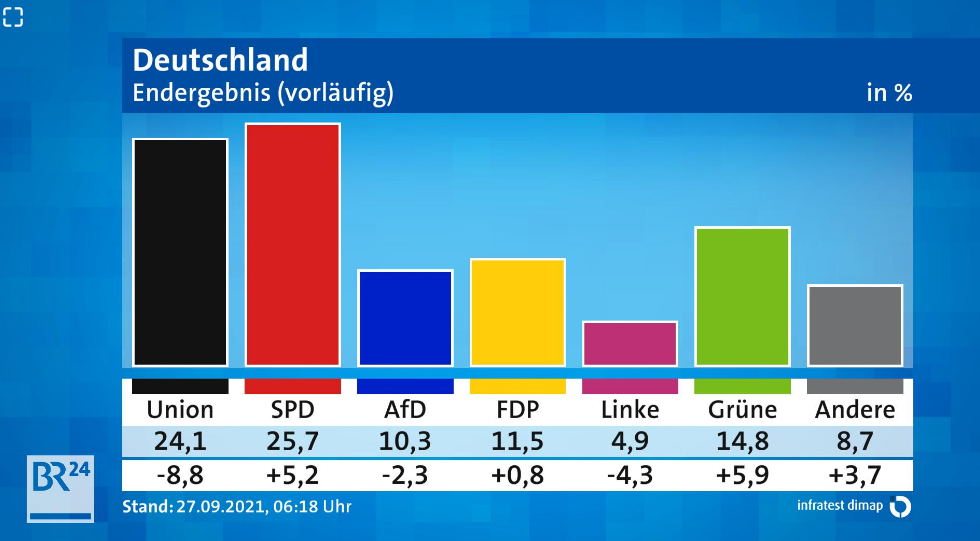
\includegraphics[width=.7\textwidth]{pics/bundestagswahl21-ergebnis.png}
\end{center}

\scriptsize\url{bundestagswahl.br.de/public/ec/ergebnis-bundestagswahl-2021-bayern-deutschland.html}
\end{frame}

\begin{frame}{Bundestagswahl 2021}
\phantomsection\label{bundestagswahl-2021-1}
Ziele:

\begin{itemize}
\tightlist
\item
  Schluss von der Befragung einer Stichprobe von Wähler:innen auf
  Gesamtergebnis
\item
  Analyse von Wahlverhalten durch weitere Fragen (Wechselwähler:innen
  etc.)
\end{itemize}
\end{frame}

\begin{frame}{Wahlfälschung}
\phantomsection\label{wahlfuxe4lschung}
Idee: Untersuche Zusammenhang zwischen Wahlergebnis (Stimmenanteil der
Sieger) und Wahlbeteiligung.\\
\emph{ballot stuffing} treibt beides in die Höhe!

\begin{center}
  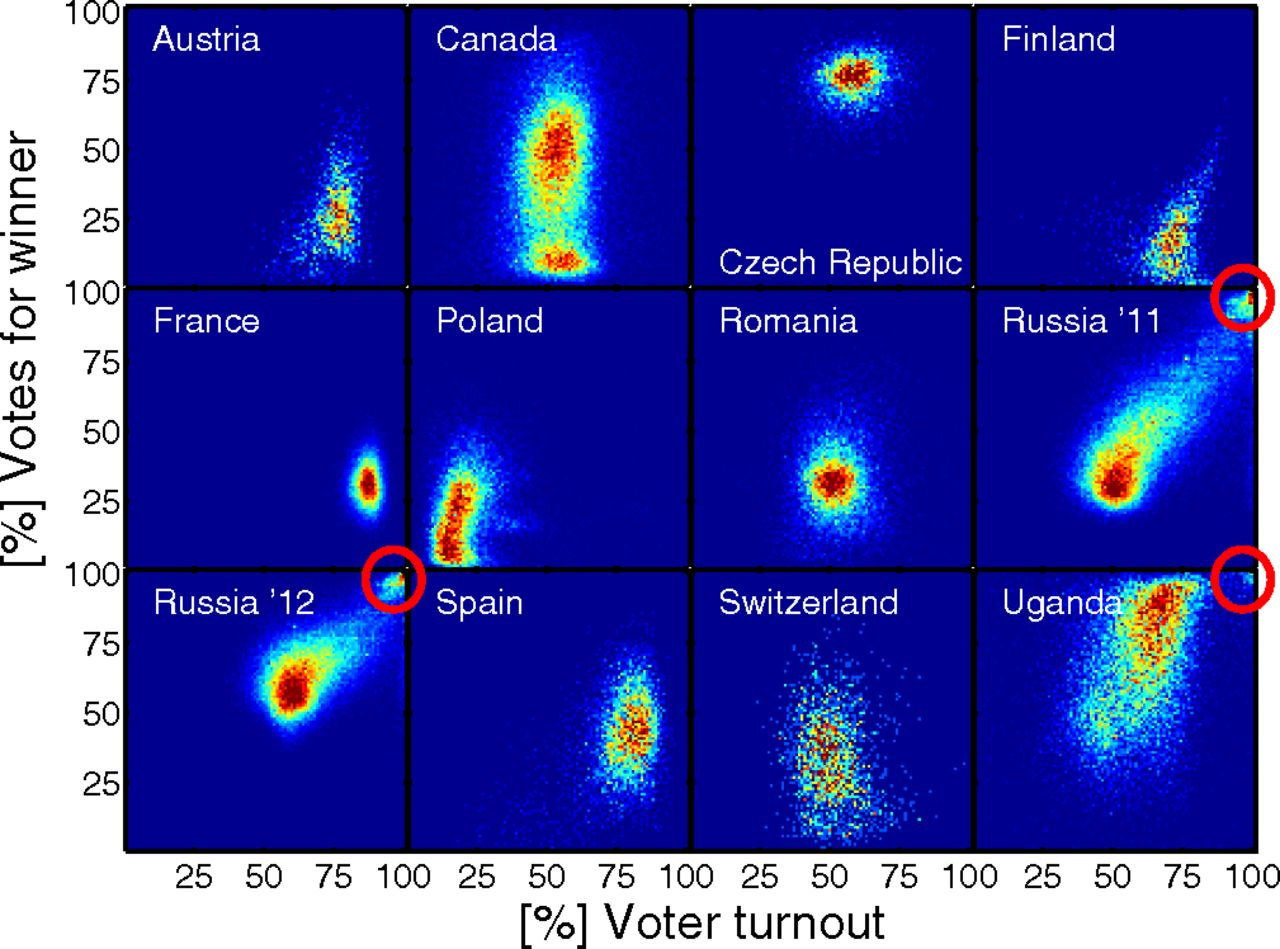
\includegraphics[width=.7\textwidth]{pics/0-ex2-electionfraud.jpg}
\end{center}
\scriptsize
\vspace{-.5em}

P. Klimek, Y. Yegorov, R. Hanel, S. Thurner (2012). Statistical
detection of systematic election irregularities. \emph{PNAS}
109(41):16469--16473.
\end{frame}

\begin{frame}{KOALA - Koalitions Analyse}
\phantomsection\label{koala---koalitions-analyse}
StaBLab-Projekt mit H. Küchenhoff, A. Bender, A. Bauer

\begin{itemize}
\tightlist
\item
  Ziel: Bessere Vermittlung der den Wahlumfragen zugrunde liegenden
  Unsicherheiten
\item
  Kleinere Änderungen in Umfrageanteilen der Parteien vor Wahlen nicht
  immer relevant, teilweise überbewertet
\item
  Tatsächlich relevant sind Änderungen in der Wahrscheinlichkeit
  bestimmter Ereignisse nach Wahlen (Wahrscheinlichkeit für
  Zustandekommen von Mehrheiten für Koalitionen)
\item
  Basis: Simulation vieler möglicher Wahlergebnisse auf Basis (mehrerer)
  aktueller Umfragen
\item
  Wahrscheinlichkeit: Anteil der Simulationen in welchen Ereignis
  eintritt
\end{itemize}

\vspace{.5cm}

Website:
\href{https://koala.stat.uni-muenchen.de/}{koala.stat.uni-muenchen.de}
\end{frame}

\begin{frame}{KOALA - Koalitions Analyse}
\phantomsection\label{koala---koalitions-analyse-1}
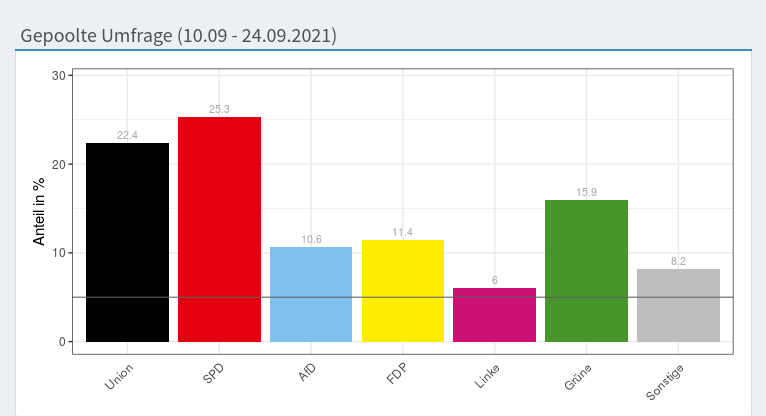
\includegraphics{pics/koala_survey}
\end{frame}

\begin{frame}{KOALA - Koalitions Analyse}
\phantomsection\label{koala---koalitions-analyse-2}
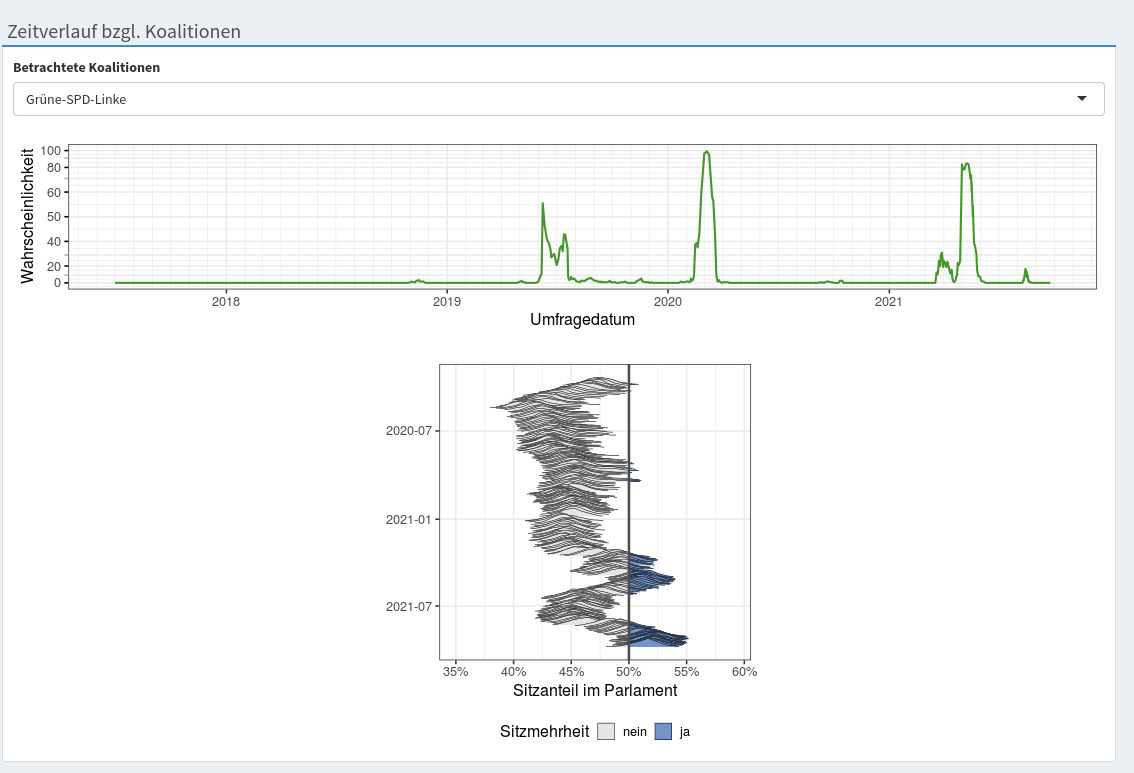
\includegraphics{pics/koala_probs}
\end{frame}

\begin{frame}{ISAR - Lebensmittelimportscreening}
\phantomsection\label{isar---lebensmittelimportscreening}
StaBLab-Projekt mit H. Küchenhoff, A. Bauer und F. Günther in
Zusammenarbeit mit Bayrischem Landesamt für Gesundheit und
Lebensmittelsicherheit, sowie Bundesamt für Verbraucherschutz und
Lebensmittelsicherheit

\begin{itemize}
\tightlist
\item
  Ziel: Früherkennung von Risiken im Lebensmittelhandel
\item
  Ansatz: Dauerhaftes Screening von produkt- und länderspezifischen
  Daten aller deutscher Lebensmittelimporte
\item
  Auffälligkeiten in Mengen oder Preisen können Hinweise zu Risiken und
  Betrugspotentialen liefern
\item
  Ansatz: Verwendung statistischer Zeitreihen-Modelle

  \begin{itemize}
  \tightlist
  \item
    Vergleich der Beobachtungen mit Vorhersagen der Modelle
  \item
    Definition von Auffälligkeiten von Interesse
  \item
    Jeden Monat erhalten Lebensmittelkontrolleure Liste mit auffälligen
    Zeitreihen
  \end{itemize}
\item
  Programmierung von Tool zur interaktiven Darstellung der Daten in
  enger Zusammenarbeit mit Anwendern
\end{itemize}
\end{frame}

\begin{frame}{ISAR: Beispiel Haselnüsse Türkei}
\phantomsection\label{isar-beispiel-haselnuxfcsse-tuxfcrkei}
\begin{itemize}
\tightlist
\item
  2014 Ernteeinbruch von Haselnüssen in der Türkei
\item
  Darauf folgend starker Preisanstieg
\item
  Es wurden verstärkt Kontrollen der nach Deutschland importierten
  Haselnussprodukte durchgeführt
\item
  In verarbeiteten Produkten wurde Verfälschungen, u.a. durch
  Cashews/Mandeln gefunden, hohes Gesundheitsrisiko (Allergie)
\item
  In ISAR erste Signale für auffällige Preisentwicklung im September
  2015
\end{itemize}

\begin{center}
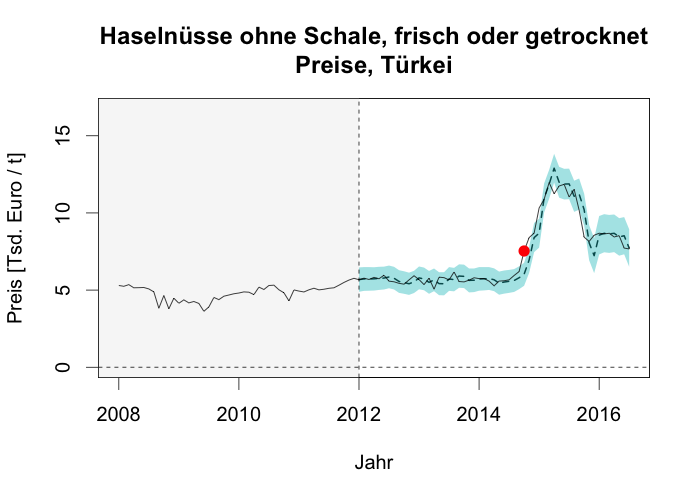
\includegraphics[width=.6\textwidth]{pics/Haselnuesse_03} \\
\end{center}
\end{frame}

\begin{frame}{ISAR: Beispiel Haselnüsse Türkei}
\phantomsection\label{isar-beispiel-haselnuxfcsse-tuxfcrkei-1}
\begin{itemize}
\tightlist
\item
  2014 Ernteeinbruch von Haselnüssen in der Türkei
\item
  Darauf folgend starker Preisanstieg
\item
  Es wurden verstärkt Kontrollen der nach Deutschland importierten
  Haselnussprodukte durchgeführt
\item
  In verarbeiteten Produkten wurde Verfälschungen, u.a. durch
  Cashews/Mandeln gefunden, hohes Gesundheitsrisiko (Allergie)
\item
  In ISAR erste Signale für auffällige Preisentwicklung im September
  2015
\end{itemize}

\begin{center}
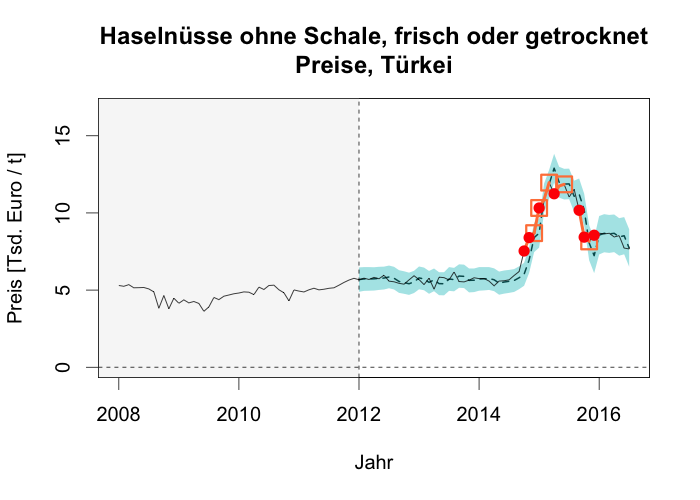
\includegraphics[width=.6\textwidth]{pics/Haselnuesse_05} \\
\end{center}
\end{frame}

\begin{frame}{Mineralwasserstudie}
\phantomsection\label{mineralwasserstudie}
Studie in Zusammenarbeit mit Prof.~O. Adam (LMU)\\
\textbf{Fragestellung:} Schmeckt mit Sauerstoff angereichertes
Mineralwasser besser als gewöhnliches Mineralwasser ?

\begin{itemize}
\tightlist
\item
  Doppel--Blindstudie
\item
  Kontroll--Gruppe: zweimal das gleiche Wasser ohne \(O_2\)
\item
  Verum--Gruppe: Beim zweiten Mal mit \(O_2\) angereichertes
  Mineralwasser
\end{itemize}

Ergebnis (Clausnitzer et al., 2004) :

\begin{itemize}
\tightlist
\item
  Placebo: 76\% gaben an, dass das zweite Wasser anders schmeckt
\item
  Verum : 89 \% gaben an, dass das zweite Wasser anders schmeckt
\end{itemize}

Signifikanter Effekt \(\rightarrow\) Zulassung
\end{frame}

\begin{frame}{Ziele und Methoden}
\phantomsection\label{ziele-und-methoden}
\begin{itemize}
\tightlist
\item
  Randomisierte Studie (Doppelblind)
\item
  Entscheidungsfindung durch statistischen Test
\item
  Quantifizierung des Effekts
\end{itemize}
\end{frame}

\begin{frame}{Umweltzone und Feinstaubbelastung}
\phantomsection\label{umweltzone-und-feinstaubbelastung}
Wirkt die Umweltzone?

Einfacher Ansatz: Vergleiche Mittelwerte vor und nach der Einführung von
Umweltzone und Fahrverbot

Probleme:

\begin{itemize}
\tightlist
\item
  Grundbelastung ohne Autoverkehr kann sich ändern
\item
  Starke Wettereinflüsse
\item
  Schwankungen über Tag und Jahreszeit
\end{itemize}

Daher: Regressionsmodell mit Referenzstation, Wetter, Tagesverlauf

\scriptsize

V. Fensterer, H. Küchenhoff, V. Maier, H.-E. Wichmann, S. Breitner, A.
Peters, J. Gu, and J. Cyrys (2014). Evaluation of the impact of low
emission zone and heavy traffic ban in Munich (Germany) on the reduction
of PM\(_{10}\) in ambient air. \emph{International Journal of
Environmental Research and Public Health} 11(5):5094-5112.
\end{frame}

\begin{frame}{Wirkung der Umweltzone: Prinzregentenstrasse}
\phantomsection\label{wirkung-der-umweltzone-prinzregentenstrasse}
\begin{center}
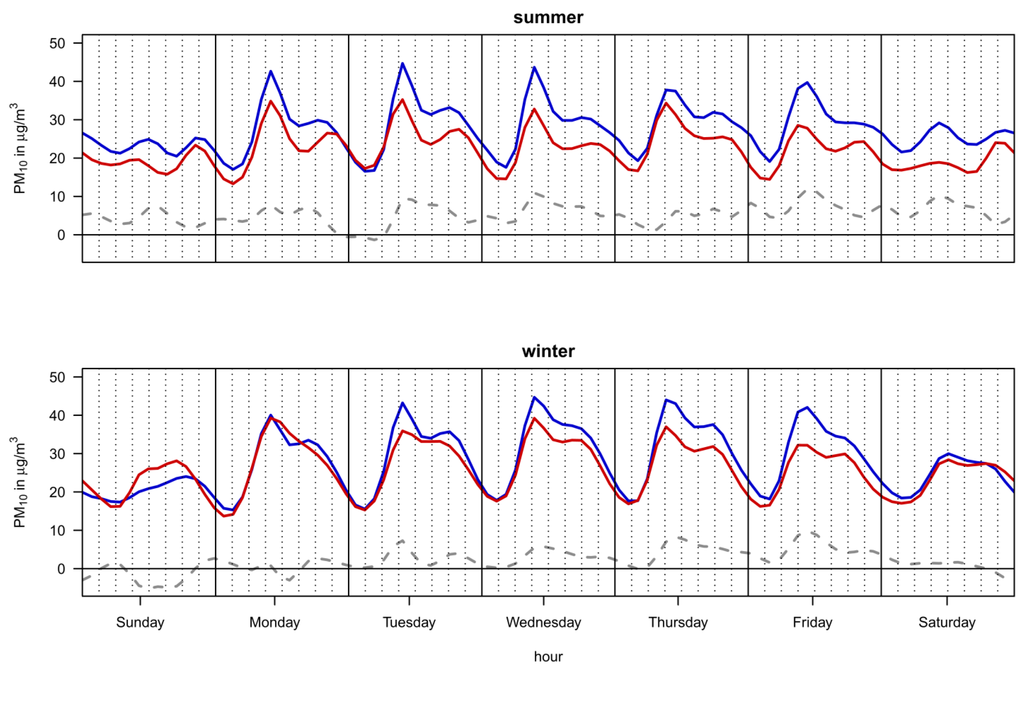
\includegraphics[height = .8\textheight]{pics/0-ex6-umweltzone-prinzregenten.png}
\end{center}
\end{frame}

\begin{frame}{Wirkung der Umweltzone: Lothstrasse}
\phantomsection\label{wirkung-der-umweltzone-lothstrasse}
\begin{center}
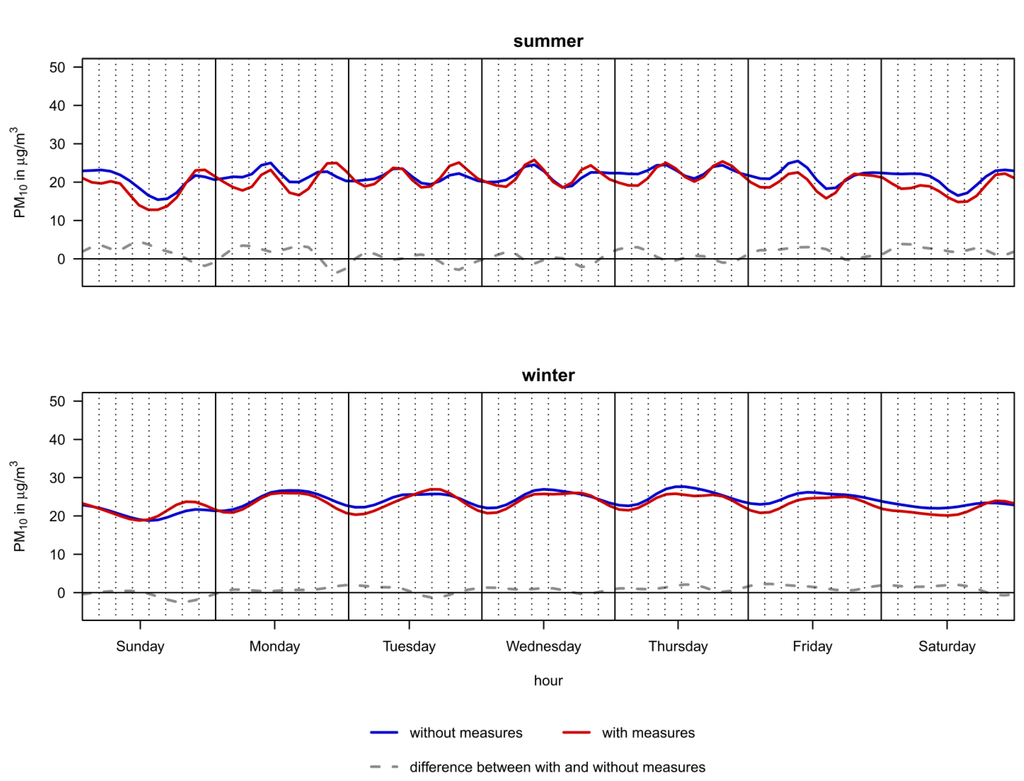
\includegraphics[height = .8\textheight]{pics/0-ex6-umweltzone-loth.png}
\end{center}
\end{frame}

\begin{frame}{Weitere Beispiele}
\phantomsection\label{weitere-beispiele}
\begin{itemize}
\tightlist
\item
  Klinische Studien
\item
  Epidemiologische Studien
\item
  Qualitätskontrolle
\item
  Marktforschung

  \begin{itemize}
  \tightlist
  \item
    Einschaltquoten
  \item
    Bewertung und Vergleich von Produkten gleichen Typs aber
    verschiedener Produzenten durch Verbraucher (Waschmittel, Kaffee,
    Schokolade, usw.)
  \item
    Online-Tracking-Daten: Cookies, Userprofile, Websitenutzung,
    \ldots{}
  \item
    A-B-Testing von Websitedesigns, User Interfaces
  \end{itemize}
\item
  Sportstatistik
\item
  Analyse von Genexpressions- oder -sequenzdaten
\item
  Netzwerkanalysen
\item
  Mustererkennung (``\,`Pattern recognition'''): Spamfilter, Customer
  Churn, Kundensegmentierung, \ldots{}
\end{itemize}
\end{frame}

\subsection{Statistik: Was - Wie -
Warum}\label{statistik-was---wie---warum}

\begin{frame}{Was ist Statistik?}
\phantomsection\label{was-ist-statistik}
\textbf{Statistik als Wissenschaft bezeichnet eine Methodenlehre, die
sich mit der Erhebung, der Darstellung, der Analyse und der Bewertung
von Daten auseinander setzt.\\
Ein zentraler Aspekt ist dabei die Modellbildung mit zufälligen
Komponenten.}

Teilgebiete:

\begin{itemize}
\item
  \textbf{Deskriptive} Statistik:\\
  Beschreibung, Zusammenfassung, Visualisierung von Daten.\\
  Techniken: Grafiken, Tabellen, Kennzahlen
\item
  \textbf{Explorative} Statistik:\\
  Suche nach Strukturen in Daten. Benutzt deskriptive und induktive
  Techniken interaktiv und iterativ.
\item
  \textbf{Induktive} Statistik: Schließt von beobachteten Daten auf
  zugrundeliegende Strukturen.\\
  Angewandte Wahrscheinlichkeitsmathematik.\\
  Techniken: Statistische Modellierung, statistische Tests.
\end{itemize}
\end{frame}

\begin{frame}{Deskriptive Statistik}
\phantomsection\label{deskriptive-statistik}
\begin{itemize}[<+->]
\tightlist
\item
  \emph{Data is merely the raw material of knowledge.}\\
  Charles Wheelan (* 1966, Autor)
\end{itemize}

\textbf{Ziel: Wahrhaftige Beschreibung von Daten mit möglichst geringem
Informationsverlust}

\begin{itemize}
\tightlist
\item
  Eigenschaften und Strukturen erkennbar machen
\item
  Grafisch und durch Kennwerte
\item
  Eindimensional und mehrdimensional
  (``\emph{uni-}/\emph{multivariat}'')
\item
  keine Rückschlüsse von beobachteter Stichprobe auf die Grundgesamtheit
  oder allgemeine Phänomene (nur \emph{Deskription}, nicht
  \emph{Inferenz})
\end{itemize}
\end{frame}

\begin{frame}{Was ist Statistik?}
\phantomsection\label{was-ist-statistik-1}
\begin{itemize}[<+->]
\tightlist
\item
  \emph{Maths is a language that you use to describe statistics, but
  really it's about collecting information and putting it in an order
  that makes sense.}\\
  Lauren Stamile (* 1976, Schauspielerin)
\item
  \emph{Statistics is the grammar of science.}\\
  Karl Pearson (1857 - 1936, Mathematiker)
\item
  \emph{Statistics is the science of learning from experience.}\\
  Bradley Efron (* 1938, Statistiker)
\end{itemize}

\begin{itemize}[<+->]
\tightlist
\item
  \(\implies\) \textbf{Statistische Methodik als unabdingbares Werkzeug
  jeder empirischen Wissenschaft.}
\end{itemize}
\end{frame}

\begin{frame}{Warum Statistik?}
\phantomsection\label{warum-statistik}
\begin{itemize}[<+->]
\tightlist
\item
  \emph{Statistics is a body of methods for making wise decisions in the
  face of uncertainty.}\\
  W. Allen Wallis (1912-1998, Statistiker \& Ökonom)\\
\item
  \emph{Cognitive psychology tells us that the unaided human mind is
  vulnerable to many fallacies and illusions because of its reliance on
  its memory for vivid anecdotes rather than systematic statistics.}\\
  Steven Pinker (* 1954, Psychologe \& Linguist)
\item
  \emph{It is the mark of a truly intelligent person to be moved by
  statistics.}\\
  George Bernard Shaw (1856 - 1950, Dramatiker)
\item
  \emph{Statistik ist für mich das Informationsmittel der Mündigen. Wer
  mit ihr umgehen kann, ist weniger leicht zu manipulieren. Der Satz
  ``Mit Statistik kann man alles beweisen'' gilt nur für die Bequemen,
  die keine Lust haben, genau hinzusehen.}\\
  Elisabeth Noelle-Neumann (1916-2010, Demoskopin)
\end{itemize}

\begin{itemize}[<+->]
\tightlist
\item
  \(\implies\) \textbf{Statistische (Aus-)Bildung um irrationales
  Handeln zu vermeiden und mit Unsicherheit vernünftig umzugehen.}
\end{itemize}
\end{frame}

\begin{frame}{Warum (nicht) Statistik?}
\phantomsection\label{warum-nicht-statistik}
\begin{itemize}[<+->]
\tightlist
\item
  \emph{All models are wrong, but some are useful.}\\
  George E. P. Box (1919 - 2013, Statistiker)
\item
  \emph{The combination of some data and an aching desire for an answer
  does not ensure that a reasonable answer can be extracted from a given
  body of data.}\\
  John Tukey (1915- 2000, Mathematiker)
\item
  \emph{If you torture the data enough, nature will always confess.}\\
  Ronald Coase (1910 - 2013, Ökonom)
\item
  \emph{There are no routine statistical questions, only questionable
  statistical routines.}\\
  David R. Cox (1924 - 2022, Statistiker)
\end{itemize}

\begin{itemize}[<+->]
\tightlist
\item
  \(\implies\) \textbf{Statistik ist komplex und ihre Ergebnisse werden
  oft missbraucht oder missinterpretiert.}
\end{itemize}
\end{frame}

\begin{frame}{Warum nicht Statistik?}
\phantomsection\label{warum-nicht-statistik-1}
\begin{itemize}[<+->]
\tightlist
\item
  \emph{Not everything that counts can be counted, and not everything
  that can be counted counts.}\\
  William Bruce Cameron (1904 - 1988, Soziologe)
\end{itemize}

\begin{itemize}[<+->]
\tightlist
\item
  \emph{Our scientific age demands that we provide definitions,
  measurements, and statistics in order to be taken seriously. Yet most
  of the important things in life cannot be precisely defined or
  measured. Can we define or measure love, beauty, friendship, or
  decency, for example?}\\
  Dennis Prager (* 1948, Radiomoderator \& Publizist)
\end{itemize}

\begin{itemize}[<+->]
\tightlist
\item
  \emph{Statistics are the triumph of the quantitative method, and the
  quantitative method is the victory of sterility and death.}\\
  Hilaire Belloc (1870 - 1953, Schriftsteller \& Historiker)
\end{itemize}

\begin{itemize}[<+->]
\tightlist
\item
  \(\implies\) \textbf{Statistik nur dort sinnvoll, wo Messbarkeit und
  Quantifizierbarkeit gegeben sind.}
\end{itemize}
\end{frame}

\begin{frame}{\ldots{} und außerdem:}
\phantomsection\label{und-auuxdferdem}
\begin{itemize}[<+->]
\tightlist
\item
  \emph{Any observed statistical regularity will tend to collapse once
  pressure is placed upon it for control purposes.}\\
  \href{https://en.wikipedia.org/wiki/Goodhart's_law}{Goodhart's Law},
  auch:\\
  \emph{``When a measure becomes a target, it ceases to be a good
  measure.''}\\
  oder\\
  \emph{``The more any quantitative social indicator is used for social
  decision-making, the more subject it will be to corruption
  pressures.''}
\end{itemize}

\begin{itemize}
\tightlist
\item
  Ähnlich auch: Präventions-Paradox, \emph{self-fullfilling/-destroying
  prophecies}
\end{itemize}

\begin{itemize}[<+->]
\tightlist
\item
  \(\implies\) \textbf{Verlässliche Messungen \& Vorhersagen in
  Systemen, die selbst Messergebnissen beeinflussen können \& von
  Vorhersagen beeinflusst werden, sind problematisch.}
\end{itemize}
\end{frame}

\subsection{Gegenwart \& Zukunft der
Statistik}\label{gegenwart-zukunft-der-statistik}

\begin{frame}{``Big Data''}
\phantomsection\label{big-data}
\begin{itemize}
\tightlist
\item
  Analyse und Verarbeitung großer Datenmengen
\item
  Drei Vs: Volume, Velocity, Variety
\item
  Häufig rein heuristische/algorithmische Herangehensweise ohne
  probabilistische Modelle oder kausale Theorien
\item
  Große Herausforderungen für Statistik und Informatik
\end{itemize}
\end{frame}

\begin{frame}{``Big Data''}
\phantomsection\label{big-data-1}
\begin{center}
       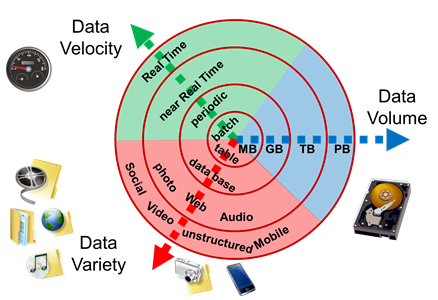
\includegraphics [width = .9\textwidth]{pics/0-bigdata.png}
 \end{center}
\end{frame}

\begin{frame}{Big Data, Machine Learning, KI}
\phantomsection\label{big-data-machine-learning-ki}
\begin{itemize}
\item
  \emph{Induktive Statistik} umfasst ``Machine Learning'' \& heutige
  ``Künstliche Intelligenz'' \(:\approx\) Methoden für Mustererkennung
  \& Vorhersagen basierend auf Daten
\item
  Alltagserfahrungen zunehmend durch datengetriebene Algorithmen
  bestimmt -- Beispiele:

  \begin{itemize}
  \tightlist
  \item
    Medien: ``filter bubble'', ``engagement maximization'' durch
    Empfehlungsalgorithmen
  \item
    Finanziell: z.B. werden verfügbare Zahlungsmethoden bei
    Online-Käufen durch Kreditscores bestimmt
  \end{itemize}
\item
  Entscheidungen großer Tragweite zunehmend durch datengetriebene
  Algorithmen -- Beispiele:

  \begin{itemize}
  \tightlist
  \item
    Kreditvergabe via Kreditscoring
  \item
    Risikoscoring der
    \href{https://github.com/corona-warn-app/cwa-documentation/blob/master/transmission_risk.pdf}{Corona-Warn-App}
  \item
    Medizinische Diagnostik und Therapievorschläge (z.B
    \href{https://www.nature.com/articles/s41598-021-84973-5}{\emph{Watson
    for Oncology}})
  \item
    \href{https://projects.tampabay.com/projects/2020/investigations/police-pasco-sheriff-targeted/intelligence-led-policing/}{``Predictive
    Policing''}
  \item
    Haftentlassung auf Bewährung - z.B. Berk, R. (2017)
    \href{https://doi.org/10.1007/s11292-017-9286-2}{\emph{Impact
    assessment of machine learning risk forecasts on parole board
    decisions and recidivism.}}
  \item
    Militärische KI:
    \href{https://venturebeat.com/2019/11/08/the-u-s-military-algorithmic-warfare-and-big-tech/}{US
    Algorithmic Warfare Initiative},
    \href{https://theintercept.com/2018/03/06/google-is-quietly-providing-ai-technology-for-drone-strike-targeting-project/}{Project
    Maven},
  \end{itemize}
\end{itemize}
\end{frame}

\begin{frame}{Big Data \& ML: Politische \& soziale Folgen}
\phantomsection\label{big-data-ml-politische-soziale-folgen}
\begin{itemize}[<+->]
\tightlist
\item
  \emph{Big data knows and can deduce more about you than Big Brother
  ever could.}\\
  Toomas Hendrik Ilves (*1953, Diplomat \& Politiker)
\end{itemize}

\begin{itemize}[<+->]
\tightlist
\item
  \emph{Arguing that you don't care about the right to privacy because
  you have nothing to hide is no different than saying you don't care
  about free speech because you have nothing to say. {[}\ldots{]}}\\
  \emph{Privacy isn't about something to hide. Privacy is about
  something to protect. And that's who you are. That's what you believe
  in. That's who you want to become. Privacy is the right to the self.
  Privacy is what gives you the ability to share with the world who you
  are on your own terms.}\\
  Edward Snowden (* 1983, Dissident)
\end{itemize}

\begin{itemize}[<+->]
\tightlist
\item
  \emph{No system of mass surveillance has existed in any society, that
  we know of to this point, that has not been abused.}\\
  Edward Snowden (* 1983, Dissident)
\end{itemize}

\begin{itemize}[<+->]
\tightlist
\item
  \(\implies\) \textbf{Bedeutet vollautomatische, allgegenwärtige,
  pausenlose Datenerfassung das Ende der Privatsphäre?}
\end{itemize}
\end{frame}

\begin{frame}{Big Data \& ML: Politische \& soziale Folgen}
\phantomsection\label{big-data-ml-politische-soziale-folgen-1}
\begin{itemize}[<+->]
\tightlist
\item
  \emph{\textbf{Predictive models are, increasingly, the tools we will
  be relying on to run our institutions, deploy our resources, and
  manage our lives.} But {[}\ldots{]} these models are constructed not
  just from data but from the choices we make about which data to pay
  attention to -- and which to leave out. Those choices are not just
  about logistics, profits, and efficiency. They are fundamentally
  moral. If we back away from them and treat mathematical models as a
  neutral and inevitable force, like the weather or the tides, we
  abdicate our responsibility. We must come together to police
  {[}\ldots{]}, tame and disarm them. My hope is that they'll be
  remembered, like the deadly coal mines of a century ago, as relics of
  the early days of this new revolution, before we learned how to bring
  fairness and accountability to the age of data.}\\
  Cathy O'Neil (Statistikerin, Zitat aus ``Weapons of Math Destruction''
  (Crown, 2016))
\end{itemize}
\end{frame}

\begin{frame}{Big Data \& ML: Politische \& soziale Folgen}
\phantomsection\label{big-data-ml-politische-soziale-folgen-2}
\begin{itemize}[<+->]
\tightlist
\item
  \emph{{[}\ldots{} M{]}any of these models encode human prejudice,
  misunderstanding, and bias into the software systems that increasingly
  manage our lives. Like gods, these mathematical models are opaque,
  their workings invisible to all but the highest priests in their
  domain: mathematicians and computer scientists. Their verdicts, even
  when wrong or harmful, are beyond dispute or appeal. And they tend to
  punish the poor and the oppressed in our society, while making the
  rich richer.}\\
  Cathy O'Neil (Statistikerin, Zitat aus ``Weapons of Math Destruction''
  (Crown, 2016))
\end{itemize}

\begin{itemize}[<+->]
\tightlist
\item
  \emph{Hidden biases in both the collection and analysis stages present
  considerable risks and are as important to the big-data equation as
  the numbers themselves. {[}\ldots{]} The fear isn't that big data
  discriminates. We already know that it does. It's that you don't know
  if you've been discriminated against.}\\
  Kate Crawford (Informatikerin)
\end{itemize}

\begin{itemize}[<+->]
\tightlist
\item
  \(\implies\) \textbf{Große Herausforderung der nächsten Jahrzehnte:
  Humane \& faire Verwirklichung der positiven Potentiale, Vermeidung
  der dystopischen Aspekte.}
\end{itemize}
\end{frame}

\begin{frame}{Gegenwart \& Zukunft der Statistik}
\phantomsection\label{gegenwart-zukunft-der-statistik-1}
\begin{itemize}
\item
  Enorm gewachsener Bedarf durch Allgegenwart automatisiert erhobener
  Daten \& Digitalisierung
\item
  Falsch/missbräuchlich angewendete Statistik führt zu
  Reproduzierbarkeitskrisen in (Sozial-)psychologie, vielen Bereichen
  der Medizin, Ernährungswissenschaften\\
  \textbf{Gegenwärtiger Paradigmenwechsel in der angewandten
  Forschung}\\
  (Stichworte: \emph{p-hacking}, \emph{replication crisis})
\item
  ``Künstliche Intelligenz'' / Maschinelles Lernen \& Big Data:
  Hochkomplexe, extrem rechenintensive Algorithmen in Kombination mit
  riesigen Datenmengen ermöglichen ganz neue Anwendungen von
  Datenanalyse\\
  \textbf{Beitrag der Statistik zur Beherrschbarmachung / Interpretation
  / Risikoabschätzung dieser Techniken?}
\end{itemize}
\end{frame}

\subsection{Theorie-Empirie-Statistik}\label{theorie-empirie-statistik}

\begin{frame}{Theorie \& Empirie}
\phantomsection\label{theorie-empirie}
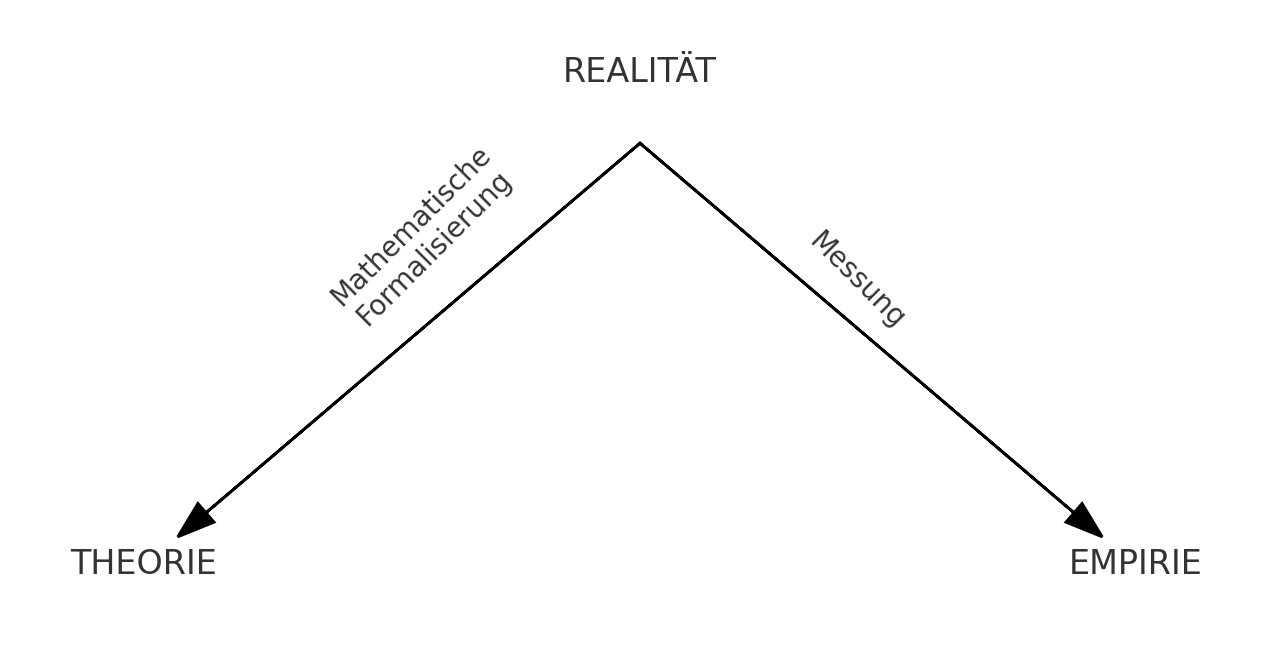
\includegraphics{pics/reality-math-data-1.png}
\end{frame}

\begin{frame}{Theorie \& Empirie}
\phantomsection\label{theorie-empirie-1}
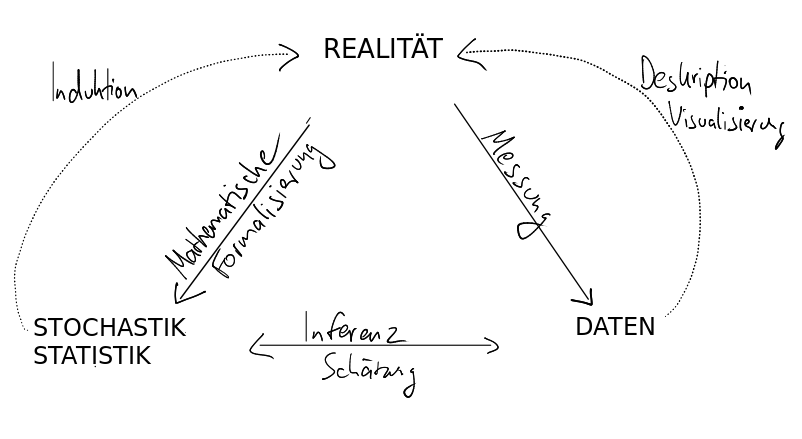
\includegraphics{pics/reality-math-data-2.png}
\end{frame}

\begin{frame}{Theorie \& Empirie}
\phantomsection\label{theorie-empirie-2}
\begin{itemize}
\item
  Modellbildung aus mathemat. Formalisierung liefert vereinfachte, grobe
  Abbildung eines Ausschnitts der Realität in Symbolen.
\item
  Daten aus Messung liefern vereinfachte, grobe Abbildung eines
  Ausschnitts der Realität in Zahlen.
\item
  Deskriptive Statistik fasst Aspekte der gemessenen Daten in
  Kennzahlen, Grafiken, Tabellen für Menschen lesbar zusammen.
\item
  Statistische Inferenz (Schätzungen \& Tests) liefert auf Basis von
  Daten quantitative Aussagen über Modell(komponenten).\\
  \textbf{Obacht: Modell \(\neq\) Realität!}
\item
  Messung selbst bzw. Definition von Messverfahren oft
  ``modellbasiert''.
\item
  Expertise für substantielle Fragestellung \emph{und} Mathe nötig um
  Realitätsnähe \& Tauglichkeit einer mathematischen Formalisierung
  beurteilen zu können.\\
  \(\implies\) sinnvolle angewandte Statistik ist \textbf{immer
  interdisziplinär}!
\end{itemize}
\end{frame}

\begin{frame}{Theorie \& Empirie}
\phantomsection\label{theorie-empirie-3}
\begin{longtable}[]{@{}
  >{\raggedright\arraybackslash}p{(\columnwidth - 4\tabcolsep) * \real{0.3333}}
  >{\raggedright\arraybackslash}p{(\columnwidth - 4\tabcolsep) * \real{0.3333}}
  >{\raggedright\arraybackslash}p{(\columnwidth - 4\tabcolsep) * \real{0.3333}}@{}}
\toprule\noalign{}
\begin{minipage}[b]{\linewidth}\raggedright
\textbf{Mathematischer Formalismus}
\end{minipage} & \begin{minipage}[b]{\linewidth}\raggedright
\end{minipage} & \begin{minipage}[b]{\linewidth}\raggedright
\textbf{Empirie / Daten}
\end{minipage} \\
\midrule\noalign{}
\endhead
Wahrscheinlichkeit & \(\xrightarrow{\textsf{verursacht(?)}}\) &
Beobachtete Häufigkeit \\
Wahrscheinlichkeit & \(\xleftarrow{\textsf{repräsentiert(?)}}\) &
Beobachtete Häufigkeit \\
& & \\
Zufallsvariable &
\(\stackrel{\textsf{entspricht}}{\longleftrightarrow}\) & Statistisches
Merkmal \\
& & \\
Erwartungswert & \(\xleftarrow{\textsf{Schätzung für}}\) &
Arithmetisches Mittel \\
& & \\
Stochastische Grundgesamtheit \(\Omega\) &
\(\stackrel{\textsf{?}}{\longleftrightarrow}\) & Statistische
Grundgesamtheit \\
& & \\
\bottomrule\noalign{}
\end{longtable}

usw.
\end{frame}

\section{Datenerhebung \& Messung}\label{datenerhebung-messung}

\begin{frame}{Grundbegriffe}
\phantomsection\label{grundbegriffe}
\begin{block}{Def.: \textbf{Statistische Einheit, Untersuchungseinheit}
(UE)}
\phantomsection\label{def.-statistische-einheit-untersuchungseinheit-ue}
Objekte, an denen interessierende Größen erfasst werden.
``Merkmalsträger''.
\end{block}

\begin{block}{Def.: \textbf{Grundgesamtheit, Population} (GG)}
\phantomsection\label{def.-grundgesamtheit-population-gg}
Menge aller für eine Fragestellung relevanten statistischen Einheiten
\end{block}

\begin{block}{Def.: \textbf{Teilgesamtheit, Stichprobe}}
\phantomsection\label{def.-teilgesamtheit-stichprobe}
Eine Teilmenge der GG, speziell: die Teilmenge an UE, für die Daten
vorliegen.
\end{block}
\end{frame}

\begin{frame}{Grundbegriffe}
\phantomsection\label{grundbegriffe-1}
\begin{block}{Def.: \textbf{Merkmal, (Ko-)Variable}}
\phantomsection\label{def.-merkmal-ko-variable}
Eine messbare Eigenschaft der Untersuchungseinheiten
\end{block}

\begin{block}{Def.: \textbf{Merkmalsausprägung}}
\phantomsection\label{def.-merkmalsauspruxe4gung}
Konkreter Wert eines Merkmals für eine bestimmte UE.
\end{block}

\begin{block}{Def.: \textbf{Merkmalsraum} (Zustandsraum)}
\phantomsection\label{def.-merkmalsraum-zustandsraum}
Menge aller \emph{möglichen} Merkmalsausprägungen eines Merkmals
\end{block}

Beachte: \emph{beobachtete} Ausprägungen \(\subseteq\) Merkmalsraum

\begin{block}{Def.: \textbf{Beobachtung}}
\phantomsection\label{def.-beobachtung}
Die Gesamtheit der beobachteten Merkmalsausprägungen der gemessenen
Merkmale einer Untersuchungseinheit zu einem bestimmten Messzeitpunkt.
\end{block}

\note{s. kasten Fahrmeir S. 15}
\end{frame}

\subsection{Messung}\label{messung}

\begin{frame}{Messen}
\phantomsection\label{messen}
\begin{itemize}[<+->]
\tightlist
\item
  \emph{Measurement is the contact of reason with nature.}\\
  Henry Margenau (1959)
\end{itemize}

\begin{itemize}[<+->]
\tightlist
\item
  \emph{In its broadest sense, measurement is the assignment of numerals
  to objects or events according to rules.}\\
  Stanley S. Stevens (1951)
\end{itemize}
\end{frame}

\begin{frame}{Messen}
\phantomsection\label{messen-1}
\textbf{Messen} bedeutet: Zuordnung von Zahlen/Symbolen zu Ausprägungen
von Merkmalen an Untersuchungseinheiten.

\begin{itemize}
\tightlist
\item
  Physikalische Messungen:\\
  Länge, Blutdruck, Temperatur, \ldots{}\\
\item
  Psychometrische Beispiele:\\
  Gewaltbereitschaft, Schwere der Depression, \ldots{}
\item
  Wirtschaftswissenschaftliche Beispiele:\\
  Inflation, Bruttosozialprodukt, Arbeitslosenquote, \ldots{}
\end{itemize}
\end{frame}

\begin{frame}{Messen}
\phantomsection\label{messen-2}
Amir \(\longrightarrow\) 1.84\\
Liz \(\longrightarrow\) 1.61\\
Feihong \(\longrightarrow\) 1.72

Jedes Merkmal definiert bestimmte \textbf{Relationen} zwischen den UE\\
Hier z.B.: ``Amir größer als Feihong größer als Liz''\\
\strut ~

Jede gültige Messung ist eine \textbf{strukturerhaltende Abbildung}
(Homomorphismus) bezüglich dieser Relationen.\\
Hier z.B.: ``Liz ist kleiner als Amir'' \(\iff\) ``\(1.61 < 1.84\)''
\end{frame}

\begin{frame}{Typen von Messungen}
\phantomsection\label{typen-von-messungen}
\begin{enumerate}
\tightlist
\item
  Messung hat reales (physikalisches) Relativ;\\
  direkte Messung: (``\emph{representational} measurement'').\\
  z.B. Länge, Gewicht, Anzahl, Blutzuckerkonzentration
\item
  Messung besitzt durch \emph{Operationalisierung} definiertes
  Relativ;\\
  indirekte/operationale Messung (``\emph{pragmatic} measurement'').\\
  z.B. Intelligenz, Schweregrad einer Krankheit, Arbeitslosenquote
\end{enumerate}

\emph{Operationalisierung} bedeutet ``Messbarmachung'', definiert genaue
Messvorschrift, Messinstrumente, etc.
\end{frame}

\subsection{Skalenniveaus}\label{skalenniveaus}

\begin{frame}{Skalen}
\phantomsection\label{skalen}
Messungen als strukturerhaltende Abbildungen\\
also: empirisches Relativ \(\cong\) numerisches Relativ ~

\textbf{Existenz:}\\
Ist die Struktur der Objekte so, dass eine strukturerhaltende Abbildung
existiert?\\
\(\implies\) Axiome von Repräsentationstheoremen müssen erfüllt sein
(z.B. Transitivität)\\
\(\implies\) Verletzt z.B. oft durch unerfüllte Annahme von
Eindimensionalität

~

\textbf{Eindeutigkeit:}\\
Gibt es mehrere zulässige Skalen?\\
(z.B. Fläche in km\(^2\) \& ha; Temperatur in °C, °F \& °K)\\
\(\implies\) gibt es zulässige (strukturerhaltende) Transformationen?
\end{frame}

\begin{frame}{Transformationen und Operationen}
\phantomsection\label{transformationen-und-operationen}
\begin{block}{Def.: \textbf{Transformation} einer Skala}
\phantomsection\label{def.-transformation-einer-skala}
Funktion, die Ausprägungen eines Merkmals auf neue Ausprägungen
abbildet.
\end{block}

in etwa: ``Skalenwechsel'', z.B:

\begin{itemize}
\tightlist
\item
  Umwandlung in andere physikalische Einheit (Temperatur: °F \(\to\) °C)
\item
  Relabeling (Beruf: ``Putzkraft'' \(\to\) ``Raumpfleger*in'')
\item
  Gruppierung (Haarfarbe: \{``braun'', ``schwarz''\} \(\to\)
  \{``dunkel''\})
\end{itemize}

\begin{block}{Def.: \textbf{Operation} auf einer Skala}
\phantomsection\label{def.-operation-auf-einer-skala}
Funktion, die Ausprägungen eines Merkmals auf der selben Skala
miteinander in Bezug setzt.
\end{block}

z.b ``\(=\) / \(\neq\)'', ``\(>\) / \(=\) / \(<\)'', Differenzen,
Quotienten etc.
\end{frame}

\begin{frame}{Skalenniveaus}
\phantomsection\label{skalenniveaus-1}
Zulässige Skalentransformationen erhalten die Struktur der empirischen
Relative, die durch Messungen repräsentiert wird.

Die Menge zulässiger Transformationen bestimmt das Skalenniveau eines
Merkmals.

Höhere Skalenniveaus erlauben eine \emph{größere} Menge von sinnvollen
\emph{Operationen auf Werten der Skala}, aber eine \emph{kleinere} Menge
an zulässigen strukturerhaltenden \emph{Transformationen der Skala} an
sich.
\end{frame}

\begin{frame}{Nominalskala}
\phantomsection\label{nominalskala}
\begin{itemize}
\tightlist
\item
  Beispiele: Religionszugehörigkeit, Wohnort, Sockenfarbe
\item
  Struktur: keine
\item
  Sinnvolle Operationen: gleich/ungleich
\item
  Erlaubte Transformationen: alle eineindeutigen Abbildungen \(f\), da
  für sie gilt: \begin{equation*}
               a = b \iff f(a) = f(b)
           \end{equation*}
\end{itemize}
\end{frame}

\begin{frame}{Ordinal- oder Rangskala}
\phantomsection\label{ordinal--oder-rangskala}
\begin{itemize}
\tightlist
\item
  Beispiele: Schulbildung, soziale Schicht, Schweregrad einer Erkrankung
\item
  Struktur:
  \href{https://de.wikipedia.org/wiki/Ordnungsrelation\#Totalordnung}{lineare
  Ordnung}
\item
  Sinnvolle Operationen: gleich/ungleich, größer/kleiner
\item
  Erlaubte Transformationen: alle streng monoton steigenden Abbildungen
  \(f\), da für sie gilt: \begin{equation*}
               a<b \iff f(a) < f(b)
           \end{equation*}
\end{itemize}
\end{frame}

\begin{frame}{Intervallskala}
\phantomsection\label{intervallskala}
\begin{itemize}
\tightlist
\item
  Beispiele: Temperatur, Jahreszahlen, IQ
\item
  Struktur: \textbf{Abstände} quantifizierbar
\item
  Sinnvolle Operationen: gleich/ungleich, größer/kleiner,
  \textbf{Differenzbildung}
\item
  Erlaubte Transformationen: alle linearen Transformationen
  \(f(x) = ax+b,\, a > 0\), da für sie gilt: \begin{equation*}
               f(x_1) - f(x_2) = f(x_3) - f(x_4) \iff x_1 - x_2 = x_3 - x_4
           \end{equation*}
\end{itemize}
\end{frame}

\begin{frame}{Verhältnisskala}
\phantomsection\label{verhuxe4ltnisskala}
Intervallskala mit (natürlichem) Nullpunkt

\begin{itemize}
\tightlist
\item
  Beispiele: Zeitdauer, Preise, Längen, Gewichte
\item
  Struktur: Abstände quantifizierbar und \textbf{Nullpunkt} eindeutig
  festgelegt
\item
  Sinnvolle Operationen: gleich/ungleich, größer/kleiner, Differenzen,
  \textbf{Verhältnisse}
\item
  Erlaubte Transformationen: Multiplikation/Reskalierung mit
  \(f(x) = ax,\, a > 0\), da für sie gilt: \begin{equation*}
               \frac{f(x_1)}{f(x_2)} = \frac{x_1}{x_2}
           \end{equation*}
\end{itemize}
\end{frame}

\begin{frame}{Absolutskala}
\phantomsection\label{absolutskala}
\begin{itemize}
\tightlist
\item
  Beispiel: Häufigkeit, Anzahl
\item
  Struktur: Einheit liegt auf natürliche Weise fest
\item
  Erlaubte Transformationen: keine
\end{itemize}
\end{frame}

\begin{frame}{Skalenniveau}
\phantomsection\label{skalenniveau}
Beachte:

\begin{itemize}
\tightlist
\item
  Je höher das Skalenniveau, desto mehr Rechenoperationen können mit den
  beobachteten Werten sinnvoll durchgeführt werden.
\item
  Nur Rechenoperationen, deren inhaltliche Ergebnisse nicht von den
  zulässigen Transformationen der Skala beeinflusst werden, sind
  \emph{sinnvoll} interpretierbar.
\end{itemize}

Zusammenfassung:

\begin{table}
\small
\begin{tabular}{cc|cccc}
Überbegriff &  Skalenniveau & ausz\"{a}hlen & ordnen & Differenzen & Quotienten \\ \hline
qualitativ & Nominal & $\checkmark$ & \textcolor{red}{X} & \textcolor{red}{X} & \textcolor{red}{X} \\
          & Ordinal & $\checkmark$ & $\checkmark$ & \textcolor{red}{X} & \textcolor{red}{X} \\ \hline
quantitativ/ &  Intervall & $\checkmark$ & $\checkmark$ & $\checkmark$ & \textcolor{red}{X} \\
metrisch    & Verh\"{a}ltnis & $\checkmark$ & $\checkmark$ & $\checkmark$ & $\checkmark$ \\
        & Absolut & $\checkmark$ & $\checkmark$ & $\checkmark$ & $\checkmark$ \\
\end{tabular}
\end{table}

Sonderfall: dichotome, binär codierte (``0''/``1'') Merkmale sind
nominalskaliert, aber z.B. ihr Mittelwert ist sinnvoll interpretierbar.
\end{frame}

\begin{frame}{Skalentransformationen}
\phantomsection\label{skalentransformationen}
Beispiel: Konzentration von Bakterien

\begin{table}
\begin{tabular}{lcl}
$0.003$ && $\log_{10}(3.0 \cdot 10^{-3}) \approx -2.5$ \\
$0.0003$ &oder& $\log_{10}(3.0 \cdot 10^{-4})\approx -3.5$ \\
$0.00003$ && $\log_{10}(3.0 \cdot 10^{-5})\approx -4.5$
\end{tabular}
\end{table}

Skalenwahl \(\iff\) Interpretation der Differenz

Also: Inhaltlich sinnvoll, theoretisch nicht zulässig!\footnote<.->{Willkommen
  in der wunderbaren Welt der angewandten Statistik\ldots{}}

Bei \(\log\)-Skala: Differenz = \(\log\)(Faktor der Veränderung)\\
Oft: Verwende \(\log\) zur Basis 10 oder 2
\end{frame}

\begin{frame}{Indexbildung}
\phantomsection\label{indexbildung}
Zusammenfassung verschiedener Merkmale (\emph{Items}) zu einem
aggregierten Merkmal (\emph{Score}, \emph{Index}).

Häufig: Bildung von (gewichteten) Summen

Beispiel: Wahl-O-Mat\\
\(\text{Übereinstimmung SPD} = w_1 \cdot Q(\text{Tempolimit}) + w_2 \cdot Q(\text{Verteidigungsausgaben}) + ...\)
~

Indexbildung meist theoriegeleitet bzw. nach fachspezifischen
Überlegungen\\
Häufige Problematik:

\begin{itemize}
\tightlist
\item
  Gewichtung der Items?
\item
  Skalenniveau des Index?
\end{itemize}
\end{frame}

\begin{frame}{Indexbildung: Likert-Skalen}
\phantomsection\label{indexbildung-likert-skalen}
\begin{center}
       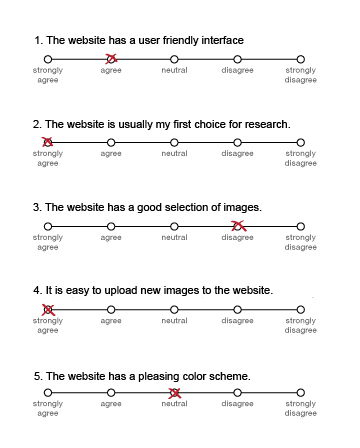
\includegraphics [height = .8\textheight]{pics/1-Example_Likert_Scale.jpg}
\end{center}

\{\scriptsize Bild: Nicholas Smith, CC BY-SA 3.0, via Wikimedia
Commons\}
\end{frame}

\begin{frame}{Indexbildung: Likert-Skalen}
\phantomsection\label{indexbildung-likert-skalen-1}
Häufig verwendetes Verfahren in der Pychometrie:

\begin{itemize}
\tightlist
\item
  Items sind Ratingskalen die Zustimmung/Ablehnnung zu bestimmten
  Aussagen zum selben Thema abfragen
\item
  Skalenwert der Likert-Skala als Summen- oder Durchschnittsscore der
  (ordinalen!) Ratings der verschiedenen Items
\end{itemize}
\end{frame}

\begin{frame}{Merkmalstypen: Stetige und diskrete Merkmale}
\phantomsection\label{merkmalstypen-stetige-und-diskrete-merkmale}
\begin{itemize}
\tightlist
\item
  \textbf{Diskretes} Merkmal:\\
  nur endlich oder abzählbar unendlich viele verschiedene Werte
  möglich\\
  z.B. Geschlecht, Kinderanzahl
\item
  \textbf{Stetiges} Merkmal:\\
  alle Werte in einem Kontinuum möglich\\
  z.B. Zeitdauer, Größe, Gewicht
\end{itemize}

Wichtige Unterscheidung für Wahl geeigneter grafischer
Darstellungsformen \& numerischer Zusammenfassungen.
\end{frame}

\begin{frame}{Weitere Klassen}
\phantomsection\label{weitere-klassen}
\begin{itemize}
\tightlist
\item
  \textbf{Quasi-stetiges} Merkmal:\\
  diskret, sehr kleine Einheiten, ``praktisch'' stetig.\\
  Beispiel: Monetäre Größen in Cent\\
  (Real existierende Messungen immer quasi-stetig wegen beschränkter
  Auflösung des Messinstruments \& der Gleitkommazahlendarstellung im
  Rechner.)
\item
  \textbf{Gruppierte} Daten, \textbf{Häufigkeits}daten:\\
  Wertebereich eines (quasi-)stetigen Merkmals wird in Gruppen (Klassen,
  Kategorien) eingeteilt.\\
  Beispiele: Gehalt in Gehaltsklassen, Alter in Altersklassen\\
  Bemerkung: Gruppierung dient auch dem Datenschutz!
\end{itemize}
\end{frame}

\subsection{Datenerhebung}\label{datenerhebung}

\begin{frame}{Erhebungsarten: Umfang}
\phantomsection\label{erhebungsarten-umfang}
\begin{block}{Def.: \textbf{Vollerhebung}}
\phantomsection\label{def.-vollerhebung}
Alle statistischen Einheiten einer Grundgesamtheit werden untersucht
(``erhoben'').
\end{block}

\begin{block}{Def.: \textbf{Stichprobe}}
\phantomsection\label{def.-stichprobe}
Auch \emph{Teilerhebung}. Ein Teil der Untersuchungseinheiten in einer
Grundgesamtheit wird untersucht. Ist die Auswahl dieser UE zufällig,
spricht man von einer \textbf{Zufallsstichprobe}.
\end{block}

Induktive Statistik ist in der Regel nur auf Basis geeigneter
\emph{Zufallsstichproben} zulässig!
\end{frame}

\begin{frame}{Erhebungsarten: Datenform}
\phantomsection\label{erhebungsarten-datenform}
\begin{block}{Def.: \textbf{Querschnittsdaten:}}
\phantomsection\label{def.-querschnittsdaten}
Ein oder mehrere verschiedene \emph{Merkmale} werden an mehreren
\emph{Untersuchungseinheit} einmal erhoben (zu einem bestimmten
Zeitpunkt oder über einen bestimmten Zeitraum).\\
Also: \textbf{Eine} \emph{Beobachtung} pro \emph{Untersuchungseinheit.}
\end{block}

\begin{block}{Def.: \textbf{Zeitreihe:}}
\phantomsection\label{def.-zeitreihe}
Ein bestimmtes \emph{Merkmal} wird wiederholt für die selbe
\emph{Untersuchungseinheit} erhoben (üblicherweise in regelmäßigen
Abständen).\\
Also: \textbf{Mehrere} \emph{Beobachtungen} \textbf{einer}
\emph{Untersuchungseinheit.}
\end{block}

\textbackslash vskip -.5em z.B. Aktienkurs eines Unternehmens,
Corona-Inzidenz in einem Landkreis

\begin{block}{Def.: \textbf{Längsschnittdaten} (auch: Longitudinal-,
Paneldaten):}
\phantomsection\label{def.-luxe4ngsschnittdaten-auch-longitudinal--paneldaten}
Die selben \emph{Merkmale} werden mehrmals zu verschiedenen Zeitpunkten
an mehreren \emph{Untersuchungseinheiten} erhoben.\\
Also: Jeweils \textbf{mehrere} \emph{Beobachtungen} \textbf{mehrerer}
\emph{Untersuchungseinheiten.}
\end{block}
\end{frame}

\begin{frame}{Erhebungsarten: Methoden operationaler Messungen}
\phantomsection\label{erhebungsarten-methoden-operationaler-messungen}
\begin{itemize}
\tightlist
\item
  Beobachtung:

  \begin{itemize}
  \tightlist
  \item
    verdeckt oder teilnehmend
  \item
    systematisch mit Beobachtungsprotokoll
  \end{itemize}
\item
  Befragung:

  \begin{itemize}
  \tightlist
  \item
    (fern)mündlich mit/ohne Interviewer, oder schriftlich/online
  \item
    Fragebogen
  \end{itemize}
\item
  Experiment

  \begin{itemize}
  \tightlist
  \item
    kontrollierte Situation, evtl. Erhebung durch Beobachtung oder
    Befragung
  \end{itemize}
\end{itemize}
\end{frame}

\begin{frame}{Experimente}
\phantomsection\label{experimente}
Es werden in der Regel verschiedene ``Behandlungen'' verglichen.

Gemeinsamkeit: Experimenteller Eingriff ins Geschehen

\begin{itemize}
\tightlist
\item
  \textbf{Randomisierte klinische Studie} : Zuordnung von Behandlungen
  zu Personen erfolgt durch Losverfahren (Randomisierung)
\item
  Randomisierte Experimente (Produktion, Landwirtschaft )\\
  Vorlesung: \emph{Versuchplanung}
\item
  Experimente in Medizin und Biologie
\item
  Naturwissenschaftliche Experimente mit zufälligen Komponenten
\item
  ``A-B-Testing'' in Web Development oder UX Design
\end{itemize}
\end{frame}

\begin{frame}{Epidemiologische Studien}
\phantomsection\label{epidemiologische-studien}
\begin{itemize}
\item
  \textbf{Kohortenstudien:}\\
  Synonym für Längsschnittdaten (\emph{retrospektiv} oder
  \emph{prospektiv})\\
  Beispiel: EPIC Studie (European Prospective Investigation into Cancer)
  400.000 Personen in neun europäischen Ländern
\item
  \textbf{Fall-Kontroll-Studien:}\\
  Erhebung von Erkrankten (Fälle) und dann dazu ``passenden'' Gesunden
  (Kontrollen)\\
  Beispiel: Deutsche Radon Studie
\end{itemize}
\end{frame}

\section{Wahrscheinlichkeit: Grundlagen \&
Definitionen}\label{wahrscheinlichkeit-grundlagen-definitionen}

\subsection{Wahrscheinlichkeit: Begriffsbildung \&
Interpretation}\label{wahrscheinlichkeit-begriffsbildung-interpretation}

\begin{frame}{Wahrscheinlichkeit}
\phantomsection\label{wahrscheinlichkeit}
Grundbegriff der Stochastik:\\
Wahrscheinlichkeit \(P(A)\) für das Auftreten eines bestimmten
Ereignisses \(A\)

\begin{align*}
P(A) & =  1           &  & A \text{ tritt mit Sicherheit ein}\\
P(A) & =  0           &  & A \text{ tritt mit Sicherheit {\em nicht} ein}\\
P(A) & =  p \in (0,1) &  & A \text{ tritt mit Wahrscheinlichkeit $p$ ein}
\end{align*}

Interpretation?

\note[item]{**NOTATION erklären!**}
\note[item]{**Interpretation fragen: Häufigkeit? Unsicherheit?**}
\end{frame}

\begin{frame}{Subjektivistische Interpretation}
\phantomsection\label{subjektivistische-interpretation}
Wahrscheinlichkeit aus Wetteinsatz:

``Wie sicher bist \emph{Du}, dass das Ereignis \(A\) eintreten wird?''\\
\(\longrightarrow\) ``Wie viel Einsatz \(e\) bist \emph{Du} maximal
bereit zu setzen, wenn beim Eintreten von \(A\) ein Gewinn \(g\)
ausgezahlt wird?'' (unter Risikoneutralität)

\[\implies P(A) = \frac{e}{g}\]

\(\implies\) Wahrscheinlichkeit als Maß für
\textbf{individuelle/subjektive Unsicherheit}.

\note[item]{Kritik: objektive W.keiten: zB Würfelwurf, statistische Mechanik; \\
wenn der gewinn hoch genug ist, dann würde man auch bei $P(A)<50\%$ spielen. }
\end{frame}

\begin{frame}{Beispiel: Sportwette}
\phantomsection\label{beispiel-sportwette}
Nick zahlt Yolanda den doppelten Einsatz als Gewinn aus, falls Yolanda's
Lieblingsteam die Meisterschaft gewinnt (Ereignis \(M\)).

\begin{itemize}
\tightlist
\item
  Nur falls Yolanda glaubt, dass \(P(M) \geq \frac12\), lässt sie sich
  auf die Wette ein.
\item
  Nick glaubt \(P(M) \leq \frac12\), sonst würde er die Wette nicht
  anbieten.
\end{itemize}
\end{frame}

\begin{frame}{Frequentistische Interpretation}
\phantomsection\label{frequentistische-interpretation}
Wahrscheinlichkeit als \textbf{Häufigkeit}:

Wenn der zufällige Vorgang beliebig oft wiederholt werden würde, dann
würde die \textbf{relative Häufigkeit} des Eintretens des Ereignisses
\(A\) gegen die Wahrscheinlichkeit \(P(A)\) konvergieren.

Klassisches Beispiel:\\
Wiederholtes Werfen eines ``fairen'' Würfels
\end{frame}

\begin{frame}{Interpretation der Interpretationen}
\phantomsection\label{interpretation-der-interpretationen}
\begin{itemize}
\item
  Für mathematische Theoriebildung weitestgehend irrelevant was
  ``\(P(A)\)'' \emph{inhaltlich} bedeutet.\\
  (Für Kommunikation und Interpretation statistischer Analysen aber
  \emph{höchst} relevant!)
\item
  Beide Interpretationen jeweils (nicht) sinnvoll für bestimmte Arten
  von Zufallsvorgängen:

  \begin{itemize}
  \tightlist
  \item
    Frequentistische Interpretation der W.keit von \emph{einzigartigen}
    Ereignissen? \ldots{} von bereits eingetretenen, aber
    \emph{unbeobachteten} Ereignissen?
  \item
    Subjektivistische Interpretation von W.keiten für einfache \&
    wiederholbare physikalische Prozesse wie Würfelwurf? \ldots{}\\
    \strut \\
  \end{itemize}
\item
  Anwendungen des subjektivistischen W.keitsbegriff:\\
  \(\to\) \textbf{Bayesianische Statistik}
\item
  Anwendungen des frequentistischen W.keitsbegriff:\\
  \(\to\) \textbf{Klassische/Frequentistische Statistik}
\end{itemize}

\note[item]{Kritik: frequentistische Interpretation von W.keiten für einzigartige Ereignisse? (z.B. ``Person X überlebt Tumor.'' oder ``Server-Auslastung am Wochenende bleibt unter 50\%'') Für Ereignisse die bereits eingetreten sind über die wir aber noch nichts wissen? (z.B. ``Wahrscheinlichkeitsverteilung'' des Absturzortes von MH370)}
\note[item]{Synthese: für praktische Arbeit \& Großteil der mathematischen Herleitung der Theorie recht egal: sowohl subjektivistische als auch objektivistische Interpretation sinnvoll/denkbar je nach Anwendung.
Mathematisch oft ineinander überführbar. Subjektivistische Interpretation $\leadsto$ Bayes)}
\end{frame}

\begin{frame}{Grundbegriffe der Stochastik}
\phantomsection\label{grundbegriffe-der-stochastik}
\begin{block}{Def.: \textbf{Ergebnisse} \(\omega\)}
\phantomsection\label{def.-ergebnisse-omega}
\(\omega\): mögliches \textbf{Ergebnis} eines Zufallsexperiments.
\end{block}

\begin{block}{Def.: \textbf{Stochastische Grundgesamtheit} \(\Omega\)}
\phantomsection\label{def.-stochastische-grundgesamtheit-omega}
Als \textbf{stochastische Grundgesamtheit} \(\Omega\) bezeichnet man die
Menge aller möglichen Ergebnisse \(\omega\) eines Zufallsexperiments.
\end{block}

Auch: ``Grundraum'', ``Basismenge'', ``Ergebnisraum''.

\begin{block}{Def.: \textbf{Ereignis}}
\phantomsection\label{def.-ereignis}
Eine Teilmenge \(A \subseteq \Omega\) heißt \textbf{Ereignis}.
\end{block}

\begin{block}{Def.: \textbf{Elementarereignisse} \(\{\omega\}\)}
\phantomsection\label{def.-elementarereignisse-omega}
Eine Teilmenge von \(\Omega\), die als einziges Element ein Ergebnis
\(\omega\) enthält, nennt man \textbf{Elementareignis}.
\end{block}

\emph{Immer nur genau ein} Elementarereignis tritt ein.

\note[item]{griechische Buchstaben einführen / nachfragen!}
\note[item]{Frage: bekannt aus Schule?}
\note[item]{Wichtig: Immer nur EIN Elementareignis kann gleichzeitig auftreten!}
\end{frame}

\subsection{Laplace-Wahrscheinlichkeiten}\label{laplace-wahrscheinlichkeiten}

\begin{frame}{Laplace-Prinzip}
\phantomsection\label{laplace-prinzip}
\emph{Prinzip von Laplace} (Pierre-Simon de Laplace {[}1749-1827{]}):

\emph{``Wenn nichts dagegen spricht, gehen wir davon aus, dass
\textbf{alle Elementarereignisse gleichwahrscheinlich} sind.''}
\end{frame}

\begin{frame}{Laplace-Wahrscheinlichkeiten}
\phantomsection\label{laplace-wahrscheinlichkeiten-1}
Betrachte die endliche Grundgesamtheit von Elementarereignissen

\[\Omega = \{\omega_1, \omega_2, ..., \omega_n \}\]

\begin{block}{Def.: Laplace-Wahrscheinlichkeit}
\phantomsection\label{def.-laplace-wahrscheinlichkeit}
Für ein \textbf{Ereignis} \(A \subseteq \Omega\) ist die
\emph{Laplace-Wahrscheinlichkeit}
\[P(A) := \frac{|A|}{|\Omega|} = \frac{|A|}{n},\] wobei \(|A|\) die
Anzahl der Elemente in \(A\) ist.
\end{block}

\(\implies\) \textbf{``Anzahl \emph{günstiger} und
gleichwahrscheinlicher Fälle durch Anzahl \emph{möglicher} und
gleichwahrscheinlicher Fälle''}

\note[item]{Notation sauber einführen: Mengenmächtigkeit, ... }
\note[item]{verbalisieren: Anzahl günstiger Fälle durch Anzahl möglicher Fälle. Nur gültig wenn alle  Fälle gleichwahrscheinlich sind.}
\end{frame}

\begin{frame}{Folgerungen und Erweiterungen}
\phantomsection\label{folgerungen-und-erweiterungen}
\begin{itemize}
\item
  Jedes Elementarereignis \(\omega_i\), \(i = 1, \ldots, n\), eines
  Laplace-W.keitsraums hat Wahrscheinlichkeit
  \(P(\{\omega_i\})=\frac{1}{n}\).
\item
  Die Wahrscheinlichkeit von \(\Omega\) ist \(P(\Omega)=1\). ~
\item
  Die entsprechende \textbf{Abbildung}
  \(P:{\mathcal P}(\Omega) \to [0,1]\) nennt man auch \textbf{diskrete
  Gleichverteilung} auf \(\Omega\)

  \begin{itemize}
  \tightlist
  \item
    \({\mathcal P}(\Omega)\) ist die \textbf{Potenzmenge} (Menge aller
    Teilmengen) von \(\Omega\) -- nicht zu verwechseln mit
    \(P(\Omega)\)!\\
    \strut ~
  \end{itemize}
\item
  Die \textbf{Vereinigung} \(U = A \cup B\) zweier Ereignisse \(A, B\)
  definiert das Ereignis\\
  ``A \emph{oder} B \emph{oder beide} treten ein''
\item
  Der \textbf{Schnitt} \(I = A \cap B\) zweier Ereignisse \(A, B\)
  definiert das Ereignis\\
  ``A \emph{und} B treten beide ein''
\end{itemize}
\end{frame}

\begin{frame}{Beispiel: Augensumme von zwei Würfeln}
\phantomsection\label{beispiel-augensumme-von-zwei-wuxfcrfeln}
\begin{align*}
\Omega &= \{(1, 1), (1, 2), ..., (6, 5), (6,6)\} \\
|\Omega| &= 6^2 =  36
\end{align*}

Sei \(A_k\) das Ereignis ``Augensumme ist \(k\)''. Dann gilt:

\[P(A_k) = \frac{6 - |k - 7|}{36}\quad\mbox{für}\quad k=2,...,12\]

\note[item]{Frage: warum nicht $\Omega =  \{(1, 1), (1, 2), ..., (1, 6), (2, 2), ..., (5, 5), (5, 6), (6,6)$ aus geordneten Tupeln mit $|\Omega| = \sum^6_{i=1} i = 15$ ? keine gleichw. Elementareignisse.}
\note[item]{
P(A_1)  & = & 0            \\
P(A_2)  & = & \frac{1}{36} \\
P(A_3)  & = & \frac{2}{36} \\
\vdots  &   & \vdots       \\
P(A_7)  & = & \frac{6}{36} \\
P(A_8)  & = & \frac{5}{36} \\
\vdots  &   & \vdots       \\
P(A_{12}) & = & \frac{1}{36}
}
\end{frame}

\begin{frame}{Interlude: Kombinatorik auf 1er Folie}
\phantomsection\label{interlude-kombinatorik-auf-1er-folie}
\emph{Wie viele unterschiedliche Möglichkeiten, \(k\) Elemente aus \(n\)
auszuwählen?}

\begin{itemize}
\item \textbf{Auswahl mit Zurücklegen, Ergebnis mit Reihenfolgen:} $$n^k$$  
   $\to$ \emph{je $n$ Möglichkeiten für alle $k$ Ziehungen}
\item \textbf{Auswahl ohne Zurücklegen, Ergebnis mit Reihenfolge:}
        $$\frac{n!}{(n-k)!} = n \cdot (n-1) \cdot \ldots \cdot (n-k+1)$$
   $\to$ \emph{zuerst $n$ Möglichkeiten, dann je $n-1$, dann je $n-2$, \dots}
\item \textbf{Auswahl ohne Zurücklegen, Ergebnis ohne Reihenfolge:}
     $$\binom{n}{k} := \frac{n!}{(n-k)!k!} = \frac{\frac{n!}{(n-k)!}}{k!}$$
   $\to$ \emph{Anzahl unterschiedlicher Auswahlen / Anzahl möglicher Reihenfolgen}
\item (\textbf{mit Zurücklegen, ohne Reihenfolge:} $\binom{n+k-1}{k}$) 
\end{itemize}
\end{frame}

\begin{frame}{Beispiel: Skatspiel}
\phantomsection\label{beispiel-skatspiel}
Beim Skatspiel werden \(32\) verschiedene Karten, darunter \(4\) Buben,
an \(3\) Personen verteilt.\\
Jede:r erhält \(10\) Karten.\\
\(2\) Karten kommen in den Skat.\\
Wie groß sind die Laplace-Wahrscheinlichkeiten der Ereignisse:

\begin{itemize}
\tightlist
\item
  \(A_1  \simeq\) ``Person 1 erhält alle Buben''
\item
  \(A_2 \simeq\) ``Alle 3 erhalten genau einen Buben''
\end{itemize}

\note[item]{
Anzahl günstige durch Anzahl mögliche: \\
günstig für A1: 4 aus 4 Buben, 6 aus den restlichen 28:\\
möglich: 10 aus 32\\
$P(A_1) = \frac{\binom{4}{4}\binom{28}{6}}{\binom{32}{10}}  =\frac{376 740}{64 512 240} = \approx 0.0058$\\
günstig für A2: Spieler 1 1 aus 4 Buben, 9 aus den restlichen 28, Spieler 2 1 aus 3 und 9 aus 19,
Spieler 3 1 aus 2 und 9 aus 10\\
möglich für A2: Spieler 1 10 aus 32, Spieler 2 10 aus 22, Spieler 3 10 aus 12.\\
$P(A_2) = \frac{\binom{4}{1}\binom{28}{9}\cdot \binom{3}{1}\binom{19}{9} \cdot \binom{2}{1}\binom{10}{9}}{\binom{32}{10}\cdot\binom{22}{10}\cdot\binom{12}{10}}  = \approx 0.056$\\
}
\end{frame}

\begin{frame}{Laplace-Wahrscheinlichkeiten sind zu speziell:}
\phantomsection\label{laplace-wahrscheinlichkeiten-sind-zu-speziell}
\vspace{-1cm}

Gegenbeispiele:

\begin{itemize}
\tightlist
\item
  Unfairer Würfel
\item
  Seltene Ereignisse, z.B. hard disk failures, Mutationen, \ldots{}
\end{itemize}

\(\leadsto\) Elementarereignisse hier nicht gleichwahrscheinlich!

\begin{itemize}
\tightlist
\item
  Außerdem: Was wenn \(|\Omega|\) unendlich?
\end{itemize}
\end{frame}

\begin{frame}{Beispiel für unendliche Grundgesamtheiten}
\phantomsection\label{beispiel-fuxfcr-unendliche-grundgesamtheiten}
Man interessiere sich für die Anzahl der Würfe einer fairen Münze bis
zum ersten Mal Zahl eintritt.
\[\Omega = \{\omega_1, \omega_2,\omega_3, \omega_4, ...  \} = \{1, 2, 3, 4, ...\} = \mathbb{N} \implies |\Omega| = \infty!\]

Allgemein mit \(\omega_i := {i}\): \begin{align*}
P(\{\omega_i\}) &= \frac{1}{2^i} \qquad i = 1, 2, 3, ...\\
\sum\limits_{i=1}^{\infty} P(\{\omega_i\}) & =  \sum\limits_{i=1}^{\infty}  \frac{1}{2^i}   \; = \;  1 \qquad
\end{align*} \footnotesize Beweis s.
\href{https://de.wikipedia.org/wiki/Geometrische_Reihe}{geom. Reihe}
\note[item]{  $P(\{\omega_i\}) = \frac{1}{2^i}$ erklären !}
\end{frame}

\subsection{Axiome von Kolmogorov}\label{axiome-von-kolmogorov}

\begin{frame}{Definitionen}
\phantomsection\label{definitionen}
\begin{block}{Def.: \textbf{Disjunkte Ereignisse}}
\phantomsection\label{def.-disjunkte-ereignisse}
\(A,B \subseteq \Omega\) sind \emph{disjunkte Ereignisse} wenn gilt:
\[A \cap B = \emptyset\].
\end{block}

\begin{block}{Def.: \textbf{Komplement/Gegenereignis}}
\phantomsection\label{def.-komplementgegenereignis}
Das \emph{Gegenereignis} oder \emph{Komplement} \(\bar A\) von
\(A \subseteq \Omega\) ist
\[\bar A := \Omega \setminus A = \{\omega \in \Omega: \omega \notin A\}\]
\end{block}

\begin{itemize}
\tightlist
\item
  Ereignis und Gegenereignis sind disjunkt.
\item
  Disjunkte Ereignisse können also nie gleichzeitig bzw. gemeinsam
  eintreten\\
  \(\implies\) \emph{Elementarereignisse} in \(\Omega\) bilden eine
  Menge von \emph{disjunkten} Ereignissen.
\end{itemize}

\note{setbuilder notation einführen}
\end{frame}

\begin{frame}{Kolmogorov-Axiome}
\phantomsection\label{kolmogorov-axiome}
Wir betrachten

\begin{itemize}
\tightlist
\item
  eine beliebige (abzählbare) Grundgesamtheit \(\Omega\)
\item
  und eine Funktion \(P\) auf der Potenzmenge \({\mathcal P}(\Omega)\),
  die jedem Ereignis \(A \subseteq \Omega\) eine Wahrscheinlichkeit
  zuordnet.
\end{itemize}

\begin{block}{Def.: \textbf{Wahrscheinlichkeitsverteilung}}
\phantomsection\label{def.-wahrscheinlichkeitsverteilung}
\(P\) ist eine \emph{Wahrscheinlichkeitsverteilung auf \(\Omega\)}, wenn
sie folgende Eigenschaften erfüllt:

\begin{itemize}
\tightlist
\item
  \textbf{A1:} \(P(A)\geq 0\) \quad für beliebige \(A \subseteq \Omega\)
  (\emph{Positivität})\\
\item
  \textbf{A2:} \(P(\Omega) = 1\) (\emph{Sicheres Ereignis})\\
\item
  \textbf{A3:} \(P(A \cup B) = P(A) + P(B)\) für \emph{disjunkte}
  Ereignisse \(A,B \subseteq \Omega\) (\emph{Additivität})
\end{itemize}
\end{block}
\end{frame}

\begin{frame}{Folgerungen}
\phantomsection\label{folgerungen}
\begin{itemize}
\tightlist
\item
  \(P(\cup_{i=1}^n\: A_i) = \sum\limits_{i=1}^n P(A_i)\) für
  \emph{paarweise disjunkte} Ereignisse
  \(A_1, A_2, ..., A_n \subset \Omega\)
\item
  \(A \subseteq B \implies P(A) \leq P(B)\)
\item
  \(P(\bar{A}) = 1 - P(A)\)
\item
  \(P(A \cup B) = P(A) + P(B) - P(A \cap B)\) für beliebige
  \(A, B \subset \Omega\)
\end{itemize}

\note[item]{
{\em Beweis $P(A) \leq P(B)$ falls $A \subseteq B$:}\\[0,3cm]
$B = B \setminus A \:\cup A $ \\
und daher \\
$P(B) \stackrel{\rm A3}{=} P(B \setminus A)
+ P(A) \stackrel{\rm A1}{\geq} P(A)$\\
}
\note[item]{mit Venn-Diagrammen grafisch zeigen!}
\note[item]{Frage: $P(\emptyset)$? }
\end{frame}

\begin{frame}{Anwendung: Siebformel von Sylvester-Poincaré}
\phantomsection\label{anwendung-siebformel-von-sylvester-poincaruxe9}
James Sylvester {[}1814-1897{]}, Jules Henri Poincaré {[}1854-1912{]}

Für beliebiges \(n \in \mathbb{N}\) und Ereignisse
\(A_1, A_2,..., A_n \subseteq \Omega\) gilt:

\begin{align*}
P(A_1 \cup A_2 \cup \dots \cup A_n) & = \sum_i P(A_i) - \sum_{i < j} P(A_i \cap A_j)\\
& \qquad + \sum_{i < j < k} P(A_i \cap A_j \cap A_k)\\
& \qquad \qquad - \dots \pm \dots \pm \dots + (-1)^{n+1} \cdot P(A_1 \cap A_2 \cap ... \cap A_n)
\end{align*}

Bsp.:\\
\begin{align*}
P(A \cup B \cup C)  =& (P(A) + P(B) + P(C))  \\
                     &  - (P(A \cap B) + P(A \cap C) + P(B \cap C)) \\
                     &    + P(A \cap B \cap C)
\end{align*}
\end{frame}

\begin{frame}{Anwendung: Bonferroni Ungleichungen}
\phantomsection\label{anwendung-bonferroni-ungleichungen}
\(\implies\) Abschätzung von \(P(A_1 \cup A_2 \cup ... \cup A_n)\)

Für beliebige Ereignisse \(A_1, A_2, ... A_n\) gilt
\[\sum_i P(A_i) \geq P\left(\bigcup_{i=1}^n A_i\right) \geq\sum_i P(A_i) - \sum_{i<j} P(A_i \cap A_j)\]

\note[item]{mit Venn-Diagrammen grafisch zeigen: summe 2er schnitte muss größer als summe 3erschnitte sein, etc.}
\end{frame}

\subsection{Bedingte
Wahrscheinlichkeiten}\label{bedingte-wahrscheinlichkeiten}

\begin{frame}{Bedingte Wahrscheinlichkeit}
\phantomsection\label{bedingte-wahrscheinlichkeit}
\begin{block}{Def.: \textbf{Bedingte Wahrscheinlichkeit}}
\phantomsection\label{def.-bedingte-wahrscheinlichkeit}
Die \emph{bedingte Wahrscheinlichkeit von \(A\) gegeben \(B\)} für
Ereignisse \(A, B \subseteq \Omega\) mit \(P(B) > 0\) ist
\[P(A|B) := \frac {P(A \cap B)}{P(B)}\]
\end{block}

Interpretation:

\begin{itemize}
\tightlist
\item
  ``Wie wahrscheinlich ist A \emph{wenn B bereits eingetreten} ist?''
\item
  ``Wie wahrscheinlich ist A \emph{unter der Annahme, dass B} der Fall
  ist?''
\end{itemize}

Intuition:

\begin{itemize}
\tightlist
\item
  ``In welchem Anteil von den Fällen, in denen \(B\) eintritt, tritt
  auch \(A\) ein?''
\item
  ``Welchen \emph{Anteil} an der Wahrscheinlichkeit für Bedingung \(B\)
  haben die Elementarereignisse, die auch Teil des interessierenden
  Ereignisses \(A\) sind?''
\end{itemize}

\note[item]{$P(A|B) :$ "W.keit für A wenn B schon eingetreten ist/unter der Annahme dass B eingetreten ist"}
\end{frame}

\begin{frame}{Beispiel: Würfelwurf}
\phantomsection\label{beispiel-wuxfcrfelwurf}
\(G:=\) ``Würfelergebnis gerade Zahl'',\\
\(F:=\) ``Würfelergebnis mindestens 5''\\
\(S:=\) ``Würfelergebnis ist 6''

Dann z.B.: \begin{align*}
\implies P(F|G) &= \frac{1}{3}\\
 P(G|F) &= \frac{1}{2} \\
 P(S|\bar G) &= 0 \\ 
 P(G|S) &= 1 \\
\end{align*}
\end{frame}

\begin{frame}{Eigenschaften von bedingten Wahrscheinlichkeiten}
\phantomsection\label{eigenschaften-von-bedingten-wahrscheinlichkeiten}
\begin{align*}
 P(B|B) & =  1 \;\; \text{(Sicheres Ereignis)}\\
 P(\bar{B}|B)& =  0 \;\;\text{(Unmögliches Ereignis)}\\
 P(A|B) & \geq 0 \mbox{ für beliebige }A \subseteq \Omega \;\; \text{(Positivität)}\\
\intertext{Außerdem gelten alle Aussagen über Wahrscheinlichkeiten \textbf{bei fester Bedingung} auch für \textit{bedingte} Wahrscheinlichkeiten, z.B.:}
P((A_1 \cup A_2)|B) & = P(A_1|B) + P(A_2|B) \mbox{ für $A_1$ und $A_2$ disjunkt. (Additivität)}  \\
\intertext{
$\implies$ Die bedingten Wahrscheinlichkeiten  $P(A|B)$ für $A \subseteq \Omega$ definieren \textit{bei fester Bedingung
$B$} einfach eine \textbf{Wahrscheinlichkeitsverteilung über die neue, kleinere stochastische Grundgesamtheit $B \subset \Omega$.}}
\intertext{Mehrfaches Bedingen $\implies$ Bedingen auf den \emph{Schnitt} der Bedingungen:}
P\big((A|B)|C \big) &= P\big(A | (B \cap C)\big) 
\end{align*}
\end{frame}

\begin{frame}{Beispiel: Skat}
\phantomsection\label{beispiel-skat}
Definiere

\(A:=\) ``Mindestens eine der acht Karokarten liegt im Skat''\\
\(B:=\) ``Spieler 1 erhält beim Austeilen keine der acht Karokarten''

Berechne \(P(A)\) und \(P(A|B)\) und vergleiche diese.

\note[item]{
&& P(A)  = 1 - P(\bar{A})\\
& = & 1 - \frac{\binom{8}{0}\binom{24}{2}}{\binom{32}{2}}\\
& = & 1 - \frac{24!/22!}{32!/30!} = 1 - \frac{24 \cdot 23}{32 \cdot 31}\\
&=& 0,4435 \\
&& P(A|B)  =  1 - P(\bar{A}|B)\\
& = & 1 - \frac{\binom{8}{0}\binom{14}{2}}{\binom{22}{2}}\\
& = & 1 - \frac{14 \cdot 13}{22 \cdot 21}\\
& = & 0,\overline{60}
"gegeben B" bedeutet 22 karten übrig, davon 8 Karo.

Alternativ: 
Omega = "alle kartenkombinationen für spieler 1 und skat"
|Omega| = \binom{32}{10}\binom{22}{2}
|\bar A \cup B| = \binom{24}{10}\binom{8}{0}\binom{14}{2}
|B| =  \binom{24}{10}\binom{22}{2}
}
\end{frame}

\begin{frame}{Multiplikationssatz}
\phantomsection\label{multiplikationssatz}
Für beliebige Ereignisse \(A_1, A_2, ..., A_n\) mit
\(P(A_1 \cap A_2 \cap ... \cap A_n) > 0\) gilt:
\[ P(A_1 \cap A_2 \cap ... \cap A_n) = P(A_1)\cdot P(A_2|A_1) \cdot P(A_3|A_1 \cap A_2) \cdot ... \cdot P(A_n|A_1 \cap ... \cap A_{n-1})\]
wobei man die rechte Seite offensichtlich auch in jeder anderen
möglichen Reihenfolge faktorisieren kann.

\textbackslash vskip 3em \small Alternative informelle Schreibweise:\\
\[P(A_1, A_2) := P(A_1 \cap A_2)\]\\
insbesondere gilt also z.B.\\
\(P(A_1 , A_2)  =  P(A_1)\cdot P(A_2|A_1)\),\\
\(P(A_1 , A_2 , A_3) = P(A_1)\cdot P(A_2|A_1) \cdot P(A_3|A_1, A_2)\),
\ldots{}

\note[item]{ Beweis: Definition bed. W.keit}
\end{frame}

\begin{frame}{Satz von der totalen Wahrscheinlichkeit}
\phantomsection\label{satz-von-der-totalen-wahrscheinlichkeit}
\begin{block}{Def: \textbf{Disjunkte Zerlegung (Partition)}}
\phantomsection\label{def-disjunkte-zerlegung-partition}
Die Mengen \(B_1, B_2, ..., B_n\) bilden eine \emph{disjunkte Zerlegung}
von \(\Omega\), falls

\begin{itemize}
\tightlist
\item
  \(B_1, B_2, ..., B_n\) paarweise disjunkt:
  \(B_i \cap B_j = \emptyset \quad \forall i \neq j\)
\item
  und \(B_1 \cup B_2 \cup ... \cup B_n = \Omega\)
\end{itemize}
\end{block}

\begin{block}{Satz von der totalen Wahrscheinlichkeit}
\phantomsection\label{satz-von-der-totalen-wahrscheinlichkeit-1}
Sei \(B_1, B_2, ..., B_n\) eine \emph{disjunkte Zerlegung} von
\(\Omega\) mit \(P(B_i) > 0\) für \(i=1,..., n\), dann gilt für jedes
\(A \subseteq \Omega\): \[ P(A) = \sum_{i=1}^n P(A|B_i) \cdot P(B_i) \]
\end{block}
\end{frame}

\begin{frame}{Wichtiger Spezialfall}
\phantomsection\label{wichtiger-spezialfall}
Insbesondere gilt \[ P(A) = P(A|B)P(B) + P(A|\bar{B})P(\bar{B})\] da
\(B, \bar{B}\) eine disjunkte Zerlegung von \(\Omega\) ist.

\note[item]{ Beweis: Definition bed. W.keit einsetzen}
\end{frame}

\subsection{Stochastische
Unabhängigkeit}\label{stochastische-unabhuxe4ngigkeit}

\begin{frame}{Stochastische Unabhängigkeit: Motivation}
\phantomsection\label{stochastische-unabhuxe4ngigkeit-motivation}
Frage: Wann sind 2 Ereignisse \(A, B\) \textbf{stochastisch unabhängig}?
~

Motivation über bedingte Wahrscheinlichkeiten:

Zwei Ereignisse \(A, B\) sind \emph{stochastisch unabhängig}, wenn
\begin{align*}
\underbrace{P(A|B)}_{\frac{P(A \cap B)}{P(B)}} & =   P(A)\\
\mbox{ bzw. } \underbrace{P(B|A)}_{\frac{P(A \cap B)}{P(A)}} & =   P(B)
\end{align*}

Intuition:

Zwei Ereignisse sind stochastisch unabhängig, wenn das Eintreten des
einen nichts an der Wahrscheinlichkeit des Eintretens des anderen
verändert.
\end{frame}

\begin{frame}{Stochastische Unabhängigkeit}
\phantomsection\label{stochastische-unabhuxe4ngigkeit-1}
\begin{block}{Def.: \textbf{Stochastische Unabhängigkeit}}
\phantomsection\label{def.-stochastische-unabhuxe4ngigkeit}
Zwei Ereignisse \(A, B\) sind \emph{stochastisch unabhängig}, wenn gilt:
\[ P(A \cap B) = P(A) \cdot P(B)\] Notation:
\(A \perp B :\iff P(A \cap B) = P(A) \cdot P(B)\)
\end{block}

\begin{itemize}
\tightlist
\item
  Voraussetzungen \(P(B) > 0\) und/oder \(P(A) > 0\) dafür nicht nötig.
\item
  Unabhängigkeit überträgt sich auf die Gegenereignisse:

  \begin{itemize}
  \tightlist
  \item
    \(A \perp B \iff \bar{A} \perp B\)
  \item
    \(A \perp B \iff A \perp \bar B\)
  \item
    \(A \perp B \iff \bar A \perp \bar B\)
  \end{itemize}
\end{itemize}

\note{
\begin{align*}
P(\bar A \cap B) &= P(B) - P(A \cap B) \\
&= P(B) - P(A)P(B)\\
&= P(B)(1 - P(A)).\\
\end{align*}
$P(A \cap \bar B)$ analog.
\begin{align*}
P(\bar A \cap \bar B) &= P(\bar A) - P(\bar A \cap B) \\
&= P(\bar A) - (P(B) - P(A \cap B)) \\
&= P(\bar A) - (1 - P(\bar B) - (1 - P(\bar A))(1 - P(\bar B)))\\
&= P(\bar A)P(\bar B).
\end{align*}
}
\end{frame}

\begin{frame}{Beispiel: Zweimaliges Würfeln}
\phantomsection\label{beispiel-zweimaliges-wuxfcrfeln}
Ein fairer Würfel wird zweimal hintereinander geworfen. Definiere

\begin{tabular}{ll}
$A:$ & "Beim 1. Würfelwurf eine Sechs" \\
$B:$ & "Beim 2. Würfelwurf eine Sechs"
\end{tabular}

Bei jedem Würfelwurf ist die Grundgesamtheit
\(\Omega = \{1,2,3,4,5,6 \}\).\\
Nach Laplace gilt \(P(A) = P(B) = \frac{1}{6}\).\\
Bei ``unabhängigem'' Werfen gilt somit \[
P(A \cap B) = P(A) \cdot P(B) = \frac{1}{36}
\]
\end{frame}

\begin{frame}{Beispiel: Zweimaliges Würfeln mit Tricks}
\phantomsection\label{beispiel-zweimaliges-wuxfcrfeln-mit-tricks}
Angenommen die Würfelwerfende legt es darauf an einen Pasch zu würfeln.
Sie kann den zweiten Wurf so steuern, dass sie mit W.keit \(0.5\) das
gleiche Ergebnis wie beim ersten Wurf würfelt. Die fünf anderen
möglichen Ergebnisse haben dann jeweils W.keit \(0.1\).

Dann ist zwar \(P(A)=\frac{1}{6}\) und auch \(P(B) = \frac{1}{6}\), aber
\[P(A \cap B)= P(A)P(B|A) = \frac{1}{6} \cdot \frac{1}{2} = \frac{1}{12}\]
Die Ereignisse \(A\) und \(B\) sind also abhängig, da \[
\frac{1}{12} = P(A \cap B) \neq P(A) \cdot P(B) = \frac{1}{36}
\]
\end{frame}

\begin{frame}{Unabhängigkeit von mehr als zwei Ereignissen}
\phantomsection\label{unabhuxe4ngigkeit-von-mehr-als-zwei-ereignissen}
Allgemeiner:

\begin{block}{Def.: \textbf{Stochastische Unabhängigkeit von mehr als
zwei Ereignissen}}
\phantomsection\label{def.-stochastische-unabhuxe4ngigkeit-von-mehr-als-zwei-ereignissen}
Ereignisse \(A_1, A_2, ..., A_n\) sind \emph{stochastisch unabhängig},
wenn für \textbf{alle Teilmengen} \(I \subseteq \{1, 2, ..., n\}\) mit
\(I = \{i_1, i_2, ..., i_k \}\) gilt: \[
P(A_{i_1} \cap A_{i_2} \cap ... \cap A_{i_k}) =
P(A_{i_1}) \cdot P(A_{i_2}) \cdot ... \cdot P(A_{i_k})
\]
\end{block}

\emph{Bemerkung:}\\
Aus paarweiser Unabhängigkeit folgt \textbf{nicht} die Unabhängigkeit
von mehr als zwei Ereignissen.
\end{frame}

\begin{frame}{Beispiel zur paarweisen Unabhängigkeit}
\phantomsection\label{beispiel-zur-paarweisen-unabhuxe4ngigkeit}
\begin{align*}
\Omega &= \{0, 1, 2, 3\} \quad \mbox{Laplace-Wahrscheinlichkeitsraum}\\
A_i &= \{0\} \cup \{i\} \quad \mbox{ mit $i = 1, 2, 3$}
\intertext{(z.B.: einmaliges Ziehen aus einer Urne mit 4 numerierten Kugeln)}  
\mbox{Dann gilt: } P(A_i) &= \frac{1}{2} \; \forall \; i \\
\mbox{ und } P(A_i \cap A_j) = P(\{0\}) &=  \frac{1}{4} = P(A_i) \cdot P(A_j) \; \forall \; i \neq j. \\
\intertext{$\implies A_i$ alle paarweise unabhängig -- Aber:}
P(A_1 \cap A_2 \cap A_3) &= P(\{0\}) = \frac{1}{4}\\
P(A_1) \cdot P(A_2) \cdot P(A_3) &= \frac{1}{8}
\end{align*} \(\implies A_1, A_2, A_3\) also \textbf{nicht} unabhängig.
\end{frame}

\begin{frame}{Bedingte Unabhängigkeit}
\phantomsection\label{bedingte-unabhuxe4ngigkeit}
\begin{block}{Def.: \textbf{Bedingte Unabhängigkeit}}
\phantomsection\label{def.-bedingte-unabhuxe4ngigkeit}
Sei \(C\) ein beliebiges Ereignis mit \(P(C)>0\). Zwei Ereignisse \(A\)
und \(B\) nennt man \textbf{bedingt unabhängig gegeben} \(C\), genau
dann wenn \[
P(A \cap B|C) = P(A|C) \cdot P(B|C).
\]
\end{block}

Notation: \((A \perp B)|C :\iff P(A \cap B|C) = P(A|C) \cdot P(B|C)\)

\begin{itemize}
\tightlist
\item
  Für feste Bedingung \(C\) gelten die selben Folgerungen wie für
  unbedingte stochastische Unabhängigkeit:\\
  \((A \perp B)|C \iff (\bar{A} \perp B)|C;\; (A \perp \bar B)|C;\; (\bar A \perp \bar B)|C\)
\item
  Aus bedingter stochastischer Unabhängigkeit folgt nicht unbedingte
  stochastische Unabhängigkeit!
\item
  Aus unbedingter stochastischer Unabhängigkeit folgt nicht bedingte
  stochastische Unabhängigkeit!
\end{itemize}
\end{frame}

\begin{frame}{Beispiel 1 zu bedingter (Un)abhängigkeit}
\phantomsection\label{beispiel-1-zu-bedingter-unabhuxe4ngigkeit}
Eine Box enthält 2 Münzen -- eine normale und eine gezinkte, die auf
beiden Seiten ``Kopf'' zeigt.\\
Eine Münze wird zufällig aus der Box gezogen und zweimal geworfen.

Definiere\\
\(A :=\) ``Kopf beim 1. Wurf'',\\
\(B :=\) ``Kopf beim 2. Wurf'',\\
\(C:=\) ``Normale Münze wurde ausgewählt''.

Dann gilt:\\
\(A \not \perp B\), aber \((A \perp B)|C\)!

Also: aus ``bedingt stochastisch unabhängig'' folgt \emph{nicht}
``stochastisch unabhängig''.
\end{frame}

\begin{frame}{Beispiel 2 zu bedingter (Un)abhängigkeit}
\phantomsection\label{beispiel-2-zu-bedingter-unabhuxe4ngigkeit}
Szenario: Einfacher Würfelwurf

Definiere Ereignisse \(A = \{1, 2\}; B = \{2, 4, 6\}; C = \{1, 4\}\).

Dann gilt: \(A \perp B\) (!), aber \((A \not \perp B)|C\)!

Also: aus ``stochastisch unabhängig'' folgt \emph{nicht} ``bedingt
stochastisch unabhängig''.
\end{frame}

\subsection{Der Satz von Bayes}\label{der-satz-von-bayes}

\begin{frame}{Der Satz von Bayes}
\phantomsection\label{der-satz-von-bayes-1}
Thomas Bayes {[}1701-1761{]}

Dieser Satz beruht auf der Asymmetrie der Definition von bedingten
Wahrscheinlichkeiten:

\begin{align*}
P(A|B) & = \frac{P(A \cap B)}{P(B)} \qquad \implies \quad
P(A \cap B) = P(A|B)P(B)\\
P(B|A) & =  \frac{P(A \cap B)}{P(A)} \qquad \implies \quad
P(A \cap B) = P(B|A)P(A)\\
& \implies P(A|B)P(B) = P(B|A)P(A)
\end{align*}
\end{frame}

\begin{frame}{Der Satz von Bayes II}
\phantomsection\label{der-satz-von-bayes-ii}
\begin{block}{Satz von Bayes}
\phantomsection\label{satz-von-bayes}
\begin{align*}
P(B|A)&= \frac{P(A|B)P(B)}{P(A)} \\
      &= \frac{P(A|B)P(B)}{P(A|B)P(B) + P(A|\bar{B})P(\bar{B})}
\end{align*}
\end{block}

Allgemeiner gilt für eine disjunkte Zerlegung \(B_1, ..., B_n\):\\
\[P(B_i|A) = \frac{P(A|B_i)P(B_i)}{\sum_{j=1}^n P(A|B_j)P(B_j)}\]
\end{frame}

\begin{frame}{Interpretation}
\phantomsection\label{interpretation}
\(P(B_i)\) als \emph{a-priori}-Wahrscheinlichkeiten:

\begin{itemize}
\tightlist
\item
  \(\approx\) Vorwissen über bzw. Plausibilität der Annahmen/Hypothesen
  \(B_i\)
\end{itemize}

\(P(A|B_i)\) als \emph{Likelihood} von A:

\begin{itemize}
\tightlist
\item
  wie plausibel ist die Beobachtung A \emph{unter der Annahme dass
  \(B_i\) der Fall ist}
\end{itemize}

\(P(B_i|A)\) \emph{a-posteriori}-Wahrscheinlichkeiten:

\begin{itemize}
\item
  Auf Basis der Beobachtung von \(A\) ändert sich die Wahrscheinlichkeit
  der Hypothese \(B_i\) von \(P(B_i)\) zu \(P(B_i|A).\)

  \(\implies\) Bayes liefert ``Update-Regel'':\\
  Wie verändert sich durch die Beobachtung von Daten \(A\) die
  Plausibilität der Vorannahme \(B_i\)?
\end{itemize}
\end{frame}

\begin{frame}{Bedeutung}
\phantomsection\label{bedeutung}
\(\implies\) Satz von Bayes liefert ein extrem mächtiges Verfahren zur\\
\emph{Umkehr der Bedingungsreihenfolge}:

\begin{itemize}
\tightlist
\item
  von \(P(A|B_i)\):\\
  ``Wie wahrscheinlich wäre es, Daten \(A\) zu beobachten \emph{falls
  \(B_i\) der Fall wäre}?''
\item
  zu \(P(B_i|A)\):\\
  ``Wie plausibel/wahrscheinlich ist \(B_i\) \emph{wenn ich Daten \(A\)
  beobachtet habe}?''
\end{itemize}

\textbf{Ermöglicht Rückschluss auf Plausibilität nicht direkt
beobachtbarer Phänomene/Modellannahmen \(B_i\), gegeben beobachtete
Daten \(A\) und Wahrscheinlichkeitsmodell \(P(A|B_i)\)}

\note[item]{anders:
$P(B_i)$ ist Vorwissen, repräsentiert Annahmen. Bayes liefert Update-Regel wie neue Information durch die Beobachtung von A unser Wissen über die $B_i$ verändert.\\}
\note[item]{Intuition: `wie wahrscheinlich ist die Kombination von A und Bi' normiert mit `wie wahrscheinlich ist A überhaupt'\\}
\end{frame}

\begin{frame}{Beispiel: Diagnostischer Test}
\phantomsection\label{beispiel-diagnostischer-test}
\(K:=\) ``Person ist krank''\\
\(T:=\) ``Test auf Krankheit ist positiv''

Gegeben:

\begin{itemize}
\tightlist
\item
  \textbf{Sensitivität} \(P(T|K)\) (``wahr-positiv''-Rate) des Tests
\item
  \textbf{Spezifität} \(P(\bar{T}|\bar{K})\) (``wahr-negativ''-Rate) des
  Tests
\item
  \textbf{Prävalenz} \(P(K)\) der Krankheit in der Population.
\end{itemize}

Für Therapieentscheidungen relevant:

\begin{itemize}
\tightlist
\item
  \(P(K|T)\) (``positiv prädiktiver Wert'')
\item
  \(P(\bar K|\bar T)\) (``negativ prädiktiver Wert'')
\end{itemize}
\end{frame}

\begin{frame}{Beispiel: Diagnostischer Test II}
\phantomsection\label{beispiel-diagnostischer-test-ii}
Gegeben: \begin{align*}
\text{Sensitivität / wahr-positiv-Rate:} \;\;P(T|K) &= 0.8 \\
\text{Spezifität / wahr-negativ-Rate:}\;\; P(\bar{T}|\bar{K}) &= 0.99 \\
\text{Prävalenz:} \;\; P(K) &= 0.001
\end{align*}

\begin{align*}
\implies P(T)  & =  P(T|K)P(K) + P(T|\bar{K})P(\bar{K})  =  \\
      & = P(T|K)P(K) + (1-P(\bar{T}|\bar{K}))(1-P(K)) \approx  0.011 \\
P(K|T) & =  \frac{P(T|K)P(K)}{P(T)} \approx  0.073 \; (!!)  \\
P(\bar{K}|\bar{T}) &\approx  0.989
\end{align*}
\end{frame}

\begin{frame}{Odds / ``Chancen''}
\phantomsection\label{odds-chancen}
Alternative Darstellung von W.keit als (Wett-)Chance\\
(z.B. 1:10 (``1 zu 10'') oder 3:1, engl. \emph{``odds''}):

\begin{columns}
\begin{column}{0.5\textwidth}
\begin{block}{Def.: \textbf{Odds} (``Chance")} 
Die Odds $\gamma(A)$ für ein Ereignis $A$ sind
$$\gamma(A) := \frac{P(A)}{1 - P(A)} \in [0, \infty]$$
\end{block}
$\implies P(A) = \frac{\gamma(A)}{1 + \gamma(A)}$
\end{column}
\begin{column}{0.5\textwidth}
\scriptsize

\begin{center}\includegraphics[width=.9\textwidth,height=.8\textheight]{main_files/figure-beamer/prob-odds-1} \end{center}

\normalsize
\end{column}
\end{columns}
\note[item]{
In manchen Quellen wird statt "Chance" auch "Risiko" verwendet.}
\note[item]{
Chance/Odds/Risiko: $\gamma = 1 = 1:1$ heisst $\pi=.5$;  $\gamma = 9 = 9:1$ heisst $\pi=.9$, $\gamma = .11 = 1:9$ heisst $\pi=.1$ etc.\\
Für $\pi \rightarrow 0$, $\pi \approx \gamma$}
\end{frame}

\begin{frame}{Satz von Bayes in Odds-Notation}
\phantomsection\label{satz-von-bayes-in-odds-notation}
\begin{alignat*}{3}
\frac{P(B|A)}{P(\bar{B}|A)} & = \frac{P(B)}{P(\bar{B})} &&\cdot \frac{P(A|B)}{P(A|\bar{B})}\\
\text{also:\;\;\;} \gamma(B|A) &= \gamma(B) &&\cdot \frac{P(A|B)}{P(A|\bar{B})}\\
\mbox{\em Posterior Odds} &=  \mbox{\em Prior Odds} &&\cdot \mbox{\em Likelihood Ratio}
\end{alignat*}

Je weiter der \emph{Likelihood Quotient} von 1 weg ist, desto
aussagekräftiger ist die Beobachtung von \(A\) bezüglich der
Plausibilität der Annahme \(B\).
\end{frame}

\begin{frame}{Bsp: Bayesianisches Update mit Odds}
\phantomsection\label{bsp-bayesianisches-update-mit-odds}
Mit \[P(T|K) = 0.8; \quad P(\bar{T}|\bar{K}) = 0.99; \quad
P(K) = 0.001\] ergibt sich: \begin{align*}
\text{Prior Odds: } \gamma(K) &= \frac{0.001}{0.999} = 0.\overline{001} = 1:999 \\
\text{Likelihood Ratio: } \frac{P(T|K)}{P(T|\bar K)} &= \frac{0.8}{0.01} = 80 = 80:1  \\
\implies\text{ Posterior Odds: } \gamma(K|T) &= \tfrac{1}{999} \cdot \tfrac{80}{1} = 0.\overline{080} \approx 1:12 !!
\end{align*} Also: Nur bei 1 von 13 positiven Test liegt tatsächlich
eine Krankheit vor\ldots.

Obacht, sehr häufiger Fehlschluss \textbf{``base-rate fallacy'\,'} --\\
verwechselt Likelihood(-Ratio) (hier: positiver Test 80-mal
wahrscheinlicher bei Kranken)\\
mit Posteriori (hier: \emph{wahr} positive Tests sind viel seltener als
falsch positive)\\
und vergisst/ignoriert Einfluss der Priori/\emph{base-rate} (hier:
1000-mal mehr Gesunde als Kranke)\ldots{} \textbf{\emph{remember your
priors!}}

\note[item]{
intuition für LQ: wieviel wahrscheinlicher/weniger wahrscheinlich ist A zu beobachten unter Annahme B als unter Annahme $\bar B$.\\
s.a. https://www.youtube.com/watch?v=BrK7X_XlGB8
}
\note[item]{$P(K) = 0.0264$; $P(T|K) = .222$; $P(T|\bar K) = 0.007$}
\end{frame}

\begin{frame}{Bsp 2: Bayes}
\phantomsection\label{bsp-2-bayes}
75\% der Mathestudierenden können Python.\\
15\% der anderen Studierenden können Python.

Von 1100 Studierenden studieren 100 Mathe.

Sei \(M:=\)``Tom studiert Mathe.''\\
Sei \(P:=\)``Tom kann Python''

Berechnen Sie \(\gamma(M|P)\) bzw \(P(M|P)\).
\end{frame}

\section{Zusammenhangsmaße für diskrete
Merkmale}\label{zusammenhangsmauxdfe-fuxfcr-diskrete-merkmale}

\subsection{Kontingenztafeln für diskrete und gruppierte
Merkmale}\label{kontingenztafeln-fuxfcr-diskrete-und-gruppierte-merkmale}

\begin{frame}{Einführung}
\phantomsection\label{einfuxfchrung-1}
Zurück zur Empirie --

Wie können wir in beobachteten Daten Aussagen über die (Un-)Abhängigkeit
von Merkmalen machen?

\(\Rightarrow\) \textbf{mehrdimensionale} oder \textbf{multivariate}
Daten
\end{frame}

\begin{frame}{Multivariate Daten}
\phantomsection\label{multivariate-daten}
\begin{itemize}
\tightlist
\item
  Stichprobe mit Untersuchungseinheiten \(i = 1, \dots, n\)
\item
  \textbf{Beobachtungen} \((x_i,y_i,z_i)\) der \textbf{Merkmale}
  \((X,Y,Z)\)
\item
  Daten \((x_1,y_1,z_1),\ldots,(x_i,y_i,z_i),\ldots,(x_n,y_n,z_n)\)\\
  (Im weiteren: Meistens nur 2 Merkmale \(X, Y\))
\item
  Fragestellungen:

  \begin{itemize}
  \tightlist
  \item
    \(X \leftrightarrow Y\): (Wie) hängen \(X\) und \(Y\) zusammen?\\
    \textbf{Assoziation}, \textbf{Korrelation}\\
    (``Sind X und Y \emph{unabhängig}?'')
  \item
    \(X \rightarrow Y\): (Wie) beeinflusst \(X\) das (Ziel-)Merkmal
    \(Y\)?\\
    \textbf{Regression}, \textbf{Kausalität} (\ldots{} nicht Teil dieses
    Kurses)
  \end{itemize}
\end{itemize}
\end{frame}

\begin{frame}{Diskrete und gruppierte Merkmale}
\phantomsection\label{diskrete-und-gruppierte-merkmale}
\begin{itemize}
\tightlist
\item
  Darstellung, Präsentation von diskreten Merkmalen \(X\) und \(Y\) mit
  den Ausprägungen
\end{itemize}

\begin{equation*}
\begin{array}{c}
a_1,\ldots,a_k \qquad \mbox{für }\,X\\
b_1,\ldots,b_m \qquad \mbox{für }\,Y
\end{array}
\end{equation*}

\begin{itemize}
\tightlist
\item
  Skalenniveau von \(X, Y\) hier beliebig; \(X, Y\) können auch
  gruppierte metrische Merkmale sein.
\item
  \emph{benutzt} wird hier allerdings nur das \emph{Nominal}skalenniveau
  der Merkmale.
\end{itemize}
\end{frame}

\begin{frame}{Kontingenztabellen}
\phantomsection\label{kontingenztabellen}
Nachwahlbefragung Bundestag 2021:

\textbackslash vskip 3em \small

\begin{center}
      \begin{tabular}{r | ccccccc | c}
          & \text{SPD} & \text{CDU/CSU} & \text{Grüne} & \text{FDP} & \text{AfD} & \text{Linke} &  \text{Rest} & $\sum$ \\ \hline
          Männer & 626 & 601 & 352 & 325 & 300 & 125 & 175 & 2504\\
          Frauen & 567 & 504 & 335 & 211 & 167 & 104 & 210 & 2098 \\ \hline
          \sum  & 1193 & 1105 & 687 & 536 & 467 & 229 & 385 & 4602  
      \end{tabular}
\end{center}

\textbackslash vskip 5em \scriptsize  Quelle: Nachwahlbefragung ARD via
\href{https://de.statista.com/statistik/daten/studie/1257090/umfrage/wahlverhalten-bei-der-bundestagswahl-nach-geschlecht/}{statista.com}
\end{frame}

\begin{frame}{Beispiel: Arbeitslosigkeit}
\phantomsection\label{beispiel-arbeitslosigkeit}
Zwei Merkmale:

\begin{itemize}
\tightlist
\item
  \(X\) Ausbildungsniveau mit den Kategorien

  \begin{itemize}
  \tightlist
  \item
    ``keine Ausbildung'\,'
  \item
    ``Lehre'\,'
  \item
    ``fachspezifische Ausbildung'\,'
  \item
    ``Hochschulabschluss'\,'
  \end{itemize}
\item
  \(Y\) Dauer der Arbeitslosigkeit mit den Kategorien

  \begin{itemize}
  \tightlist
  \item
    ``Kurzzeitarbeitslosigkeit'\,' (\(\leq\) \(6\) Monate)
  \item
    ``mittelfristige Arbeitslosigkeit'\,' (\(7\)--\(12\) Monate)
  \item
    ``Langzeitarbeitslosigkeit'\,' (\(\geq\) \(12\) Monate)
  \end{itemize}
\end{itemize}
\end{frame}

\begin{frame}{Arbeitslosigkeit}
\phantomsection\label{arbeitslosigkeit}
\small

\begin{table}[hbt]
  \begin{center}
    \leavevmode\small
    \begin{tabular}{l|ccc|c}
\multicolumn{1}{c}{}
& \multicolumn{1}{c}{Kurzzeit-}
  & \multicolumn{1}{c}{mittelfristige}
    & \multicolumn{1}{c}{Langzeit-}
    & \multicolumn{1}{c}{$\sum$}\\
\multicolumn{1}{c}{}
& \multicolumn{1}{c}{arbeitslosigkeit}
  & \multicolumn{1}{c}{Arbeitslosigkeit}
    & \multicolumn{1}{c}{arbeitslosigkeit}\\\cline{2-4}
k.A.  & 86 & 19 & 18 & 123 \\
Lehre & 170 & 43 & 20 & 233 \\
Fachspez. & 40 & 11 & 5 & 56\\
Hochschule & 28 & 4 & 3 & 35\\\cline{2-4}
\multicolumn{1}{c}{$\sum$}
& \multicolumn{1}{c}{$324$}
  & \multicolumn{1}{c}{$77$}
    & \multicolumn{1}{c}{$46$}
      & \multicolumn{1}{c}{$447$}
    \end{tabular}
    \vspace{3mm}
    \\{Ausbildungsspezifische Dauer der Arbeitslosigkeit für männliche Deutsche}
\end{center}
\end{table}
\end{frame}

\begin{frame}{Allgemeine Darstellung}
\phantomsection\label{allgemeine-darstellung}
\textbf{Kontingenztafel der absoluten Häufigkeiten:}

Eine \textbf{\((k \times m)\)-Kontingenztafel der absoluten
Häufigkeiten} besitzt die Form

\begin{displaymath}
\begin{large}
\begin{array}{c|ccc|c}
      \multicolumn{1}{c}{}
        & \multicolumn{1}{c}{b_1}
          & \dots
            & \multicolumn{1}{c}{b_m}\\\cline{2-4}
      a_1 & h_{11} & \dots & h_{1m} & h_{1\cdot}\\
      a_2 & h_{21} & \dots & h_{2m} & h_{2\cdot}\\
       \cdot & \cdot & & \cdot & \cdot \\
      a_k & h_{k1} & \dots & h_{km} & h_{k\cdot}\\\cline{2-4}
      \multicolumn{1}{c}{}
          & \multicolumn{1}{c}{h_{\cdot 1} }
            & \dots
              & \multicolumn{1}{c}{h_{\cdot m} }
                & \multicolumn{1}{c}{n}
\end{array}
\end{large}
\end{displaymath}
\end{frame}

\begin{frame}{Notation}
\phantomsection\label{notation}
\begin{center}
  \begin{tabular}{ll}
  $h_{ij} = h(a_i,b_j)$           & die absolute Häufigkeit der Kombination $(a_i,b_j)$,\\*[0.5cm]
  $h_{1\cdot},\dots,h_{k\cdot}$   & die Randhäufigkeiten von $X$ \\
  $h_{\cdot 1},\dots,h_{\cdot m}$ & die Randhäufigkeiten von $Y$ \\
  \end{tabular}
\end{center}

mit
\[h_{i\cdot} = \sum^m_{j=1} h_{ij},\qquad h_{\cdot j} = \sum^k_{i=1} h_{ij}\]

Die Kontingenztabelle gibt die gemeinsame Verteilung der Merkmale \(X\)
und \(Y\) in absoluten Häufigkeiten wieder.
\end{frame}

\begin{frame}{Kontingenztafel der relativen Häufigkeiten}
\phantomsection\label{kontingenztafel-der-relativen-huxe4ufigkeiten}
Die \textbf{\((k\times m)\)-Kontingenztafel der relativen Häufigkeiten}
hat die Form

\vspace*{1cm}

\begin{displaymath}
\begin{large}
\begin{array}{c|ccc|c}
\multicolumn{1}{c}{}
& \multicolumn{1}{c}{b_1}
  & \dots
    & \multicolumn{1}{c}{b_m}\\\cline{2-4}
a_1 & f_{11} & \dots & f_{1m} & f_{1\cdot}\\
\cdot & \cdot & & \cdot & \cdot \\
a_k & f_{k1} & \dots & f_{km} & f_{k\cdot}\\\cline{2-4}
\multicolumn{1}{c}{}
  & \multicolumn{1}{c}{f_{\cdot 1} }
    & \dots
      & \multicolumn{1}{c}{f_{\cdot m} }
        & \multicolumn{1}{c}{1}
\end{array}
\end{large}
\end{displaymath}
\end{frame}

\begin{frame}{Notation}
\phantomsection\label{notation-1}
\begin{center}
\begin{tabular}{lp{9cm}}
$f_{ij} = h_{ij}/n$ & die relative Häufigkeit der Kombination $(a_i,b_j)$, \\*[0.5cm]
$f_{i\cdot}=\sum\limits_{j=1}^m f_{ij} = h_{i\cdot}/n,$
                 & $i=1,\dots,k,$ die relativen Randhäufigkeiten zu $X$,\\*[0.5cm]
$f_{\cdot j}=\sum\limits_{i=1}^k f_{ij} = h_{\cdot j}/n,$
                 & $j=1,\dots,m$, die relativen Randhäufigkeiten zu $Y$.
\end{tabular}
\end{center}

Die Kontingenztabelle gibt die gemeinsame Verteilung von \(X\) und \(Y\)
wieder.
\end{frame}

\subsection{Bedingte Häufigkeiten}\label{bedingte-huxe4ufigkeiten}

\begin{frame}{Bedingte Häufigkeiten}
\phantomsection\label{bedingte-huxe4ufigkeiten-1}
Zusammenhang zwischen \(X\) und \(Y\) aus \textbf{gemeinsamen}
Häufigkeiten \(h_{ij}\) bzw. \(f_{ij}\) schwer ersichtlich.

Deshalb: Blick auf \textbf{bedingte} Häufigkeiten\\
\(\implies\) Verteilung eines Merkmals für festen Wert des 2. Merkmals
\end{frame}

\begin{frame}{Bedingte Häufigkeiten: Beispiel}
\phantomsection\label{bedingte-huxe4ufigkeiten-beispiel}
\textbf{Wahlverhalten nach Geschlecht, Bundestagswahl 2021:}

\begin{center}
      \begin{tabular}{r | ccccccc | c}
          & \text{SPD} & \text{CDU/CSU} & \text{Grüne} & \text{FDP} & \text{AfD} & \text{Linke} &  \text{Rest} \\ \hline
          Männer & 25 & 24 & 14 & 13 & 12 & 5 & 7  & 100\\
          Frauen & 27 & 24 & 16 & 10 &  8 & 5 & 10 & 100 \\ 
      \end{tabular}
\end{center}

Prozentzahlen für Parteipräferenz in den Schichten (Subpopulationen)
``Frauen'', ``Männer''\\
\(=\) \textbf{bedingte relative Häufigkeiten für Parteipräferenzen bei
gegebenem Geschlecht}
\end{frame}

\begin{frame}{Bedingte relative Häufigkeitsverteilung}
\phantomsection\label{bedingte-relative-huxe4ufigkeitsverteilung}
Die \textbf{bedingte Häufigkeitsverteilung von} \(Y\) \textbf{unter der
Bedingung} \(X=a_i\), kurz \(Y|X=a_i\), ist bestimmt durch
\begin{displaymath}
f_{Y|X}(b_1|a_i) = \frac{h_{i1}}{h_{i\cdot}} ,\dots, f_{Y|X}(b_m|a_i) =
\frac{h_{im}}{h_{i\cdot}}.
\end{displaymath} \vspace{0.5cm} Die \textbf{bedingte
Häufigkeitsverteilung von} \(X\) \textbf{unter der Bedingung} \(Y=b_j\),
kurz \(X|Y=b_j\), ist bestimmt durch \begin{displaymath}
f_{X|Y}(a_1|b_j) = \frac{h_{1j}}{h_{\cdot j}},\dots,f_{X|Y}(a_k|b_j) =
\frac{h_{kj}}{h_{\cdot j}}.
\end{displaymath}
\end{frame}

\begin{frame}{Bemerkung}
\phantomsection\label{bemerkung}
Wegen \begin{displaymath}
\frac{h_{i1}}{h_{i\cdot}} = \frac{h_{i1}/n}{h_{i\cdot}/n} = \frac{f_{i1}}{f_{i\cdot}}
\end{displaymath} gilt auch \begin{displaymath}
\begin{array}{c}
f_{Y|X}(b_1|a_i) = \frac{f_{i1}}{f_{i\cdot}} ,\ldots, f_{Y|X}(b_m|a_i) = \frac{f_{im}}{f_{i\cdot}} \\*[0.5cm]
f_{X|Y}(a_1|b_j) = \frac{f_{1j}}{f_{\cdot j}} ,\ldots, f_{X|Y}(a_k|b_j) = \frac{f_{kj}}{f_{\cdot j}}.
\end{array}
\end{displaymath}

\noindent  \textbf{Merksatz:}\\
Bedingte Häufigkeitsverteilungen werden durch Division der \(h_{ij}\)
bzw. \(f_{ij}\) durch die entsprechende Zeilen- bzw. Spaltensumme
gebildet.
\end{frame}

\begin{frame}{Beispiel: Wahlverhalten}
\phantomsection\label{beispiel-wahlverhalten}
\small
    \begin{center}
      \begin{tabular}{r | ccccccc | c}
          & \text{SPD} & \text{CDU/CSU} & \text{Grüne} & \text{FDP} & \text{AfD} & \text{Linke} &  \text{Rest} & $\sum$ \\ \hline
          Männer & 626 & 601 & 352 & 325 & 300 & 125 & 175 & 2504\\
          Frauen & 567 & 504 & 335 & 211 &  167 & 104 & 210 & 2098 \\ 
      \end{tabular}
\end{center}

\normalsize

\begin{itemize}
\tightlist
\item
  Zeile \(X = a_1\) (Männer)\\
  Bedingte relative Häufigkeiten für Parteipräferenz der Männer
  \(f_{Y|X}(Y = b_j | X = a_1)\):\\
  ``1.Zeile / Randhäufigkeit für Männer''\\
  \(\frac{h(a_1,b_1)}{h(a_1)} = f_{Y|X}(b_1|a_1),\ldots,\frac{h(a_1,b_j)}{h(a_1)} = f_{Y|X}(b_j|a_1) ,\ldots\)\\
  \(\frac{626}{2504} \approx 25\%, \ldots, \frac{175}{2504}\approx 7\%\)
  usw.
\item
  Zeile \(X = a_2\) (Frauen) analog, z.B.
  \(\frac{h(a_2,b_1)}{h(a_2)} = \frac{567}{2098} \approx 27\%\) usw.
\end{itemize}
\end{frame}

\begin{frame}{Bedingte und gemeinsame Häufigkeiten}
\phantomsection\label{bedingte-und-gemeinsame-huxe4ufigkeiten}
Man kann auch umgekehrt aus bedingten Häufigkeiten und Randhäufigkeiten
die gemeinsamen Häufigkeiten ausrechnen. Bei der Nachwahlbefragung aus
den bedingten Häufigkeiten und Randhäufigkeiten also z.B. \[
h(a_1) = 2504\,\,\, \mbox{Männer},\,\,\, h(a_2) = 2098 \,\,\,\mbox{Frauen}; \,\,\,n = 4602.
\]

\[
\begin{array}{lcl}
& & h(a_1)\cdot f(b_1|a_1) = h(a_1,b_1)\\
\implies & &\\
& & 2504\cdot 25\% \approx 626 \quad\mbox{usw.}
\end{array}
\]
\end{frame}

\begin{frame}{Beispiel: Arbeitslosigkeit}
\phantomsection\label{beispiel-arbeitslosigkeit-1}
\begin{displaymath}
  \begin{array}{l}
      f(b_j|a_i), \quad X = a_i, \,\,\,i=1,\ldots,4 \,\,\,\mbox{Ausbildungsniveau}
      \\*[0.5cm] \mbox{z.B.}\,\,\, \frac{86}{123} = 0.699, \,\frac{19}{123} = 0.154,\ldots
      \\*[0.5cm] \hspace*{1.5cm}\frac{170}{233} = 0.730,\ldots
      \\*[0.5cm] \hspace*{1.5cm} \mbox{usw.}
  \end{array}
\end{displaymath}

\vspace*{1cm}

Für festgehaltenes Ausbildungsniveau \((X=a_i)\) erhält man die relative
Verteilung über die Dauer der Arbeitslosigkeit durch die folgende
Tabelle.
\end{frame}

\begin{frame}{Bedingte Verteilung}
\phantomsection\label{bedingte-verteilung}
\begin{center}
  \begin{small}
   \begin{tabular}{l|ccc|c}
\multicolumn{1}{c}{}
& \multicolumn{1}{c}{Kurzzeit-}
  & \multicolumn{1}{c}{mittelfristige}
    & \multicolumn{1}{c}{Langzeit-}\\
\multicolumn{1}{c}{}
& \multicolumn{1}{c}{arbeitslosigkeit}
  & \multicolumn{1}{c}{Arbeitslosigkeit}
    & \multicolumn{1}{c}{arbeitslosigkeit}\\\cline{2-4}
Keine Ausb.     & 0.699 & 0.154 & 0.147 & 1\\
Lehre                & 0.730 & 0.184 & 0.086 & 1\\
Fachspez. Aus. & 0.714 & 0.197 & 0.089 & 1\\
Hochschula.    & 0.800 & 0.114 & 0.086 & 1\\\cline{2-4}
    \end{tabular}
   \end{small}
  \end{center}

\begin{itemize}
\tightlist
\item
  Bedingen auf das Ausbildungsniveau:\\
  \(\implies\) Verteilung der Dauer der Arbeitslosigkeit für die
  Subpopulationen \grqq Keine Ausbildung\grqq, \grqq Lehre\grqq, usw.
\item
  Verteilungen lassen sich nun miteinander vergleichen
\end{itemize}

\(\implies\) Relative Häufigkeit für Kurzzeitarbeitslosigkeit ist in der
Subpopulation \grqq Hochschulabschluss\grqq~mit \(0.8\) am größten.
\end{frame}

\begin{frame}{Darstellung der bedingten Verteilung}
\phantomsection\label{darstellung-der-bedingten-verteilung}
Zum Beispiel Stapeldiagramme:

\scriptsize

\begin{center}\includegraphics[width=.9\textwidth,height=.8\textheight]{main_files/figure-beamer/03-conditional-freq-1} \end{center}

\normalsize
\end{frame}

\subsection{Diskrete Zusammenhangsanalyse:
Odds}\label{diskrete-zusammenhangsanalyse-odds}

\begin{frame}{Zusammenhangsanalyse in Kontingenztabellen}
\phantomsection\label{zusammenhangsanalyse-in-kontingenztabellen}
\emph{Bisher:} Tabellarische / grafische Präsentation\\
\emph{Jetzt:} Maßzahlen für Stärke des Zusammenhangs zwischen \(X\) und
\(Y\).

\textbf{Chancen und relative Chancen:}

\begin{itemize}
\tightlist
\item
  Betrachte zunächst nur \(2 \times 2\) - Kontingenztafeln
  \begin{displaymath}
   \begin{array}{cc|cc|c}
   & \multicolumn{1}{c}{}
     & \multicolumn{2}{c}{$Y$}\\
   & \multicolumn{1}{c}{}
     & 1
    & \multicolumn{1}{c}{2} \\\cline{3-4}
   & 1
     & h_{11}
    & h_{12}
      & h_{1\cdot}\\
   \raisebox{1.5ex}[-1.5ex]{$X$}
   & 2
     & h_{21}
    & h_{22}
      & h_{2\cdot}\\\cline{3-4}
   & \multicolumn{1}{c}{}
     &\multicolumn{1}{c}{h_{\cdot 1}}
    & \multicolumn{1}{c}{h_{\cdot 2} }
      & \multicolumn{1}{c}{n}
   \end{array}
   \end{displaymath}
\end{itemize}
\end{frame}

\begin{frame}{Odds (Chancen)}
\phantomsection\label{odds-chancen-1}
\begin{itemize}
\tightlist
\item
  Wir betrachten die Merkmale \(X\) und \(Y\) zunächst asymmetrisch: Die
  Ausprägungen von \(X\) definieren (hier 2) Subpopulationen, \(Y\) ist
  das interessierende dichotome Merkmal in diesen Subpopulationen
\item
  Unter einer \textbf{Chance} (\emph{odds}) versteht man nun das
  \textbf{Verhältnis der Häufigkeiten} von \(Y=1\) und \(Y=2\).
\item
  \textbf{bedingte Odds}: Verhältnis der bedingten Häufigkeiten von
  \(Y=1\) und \(Y=2\) \textbf{in einer Subpopulation} \(X=a_i\).
\end{itemize}
\end{frame}

\begin{frame}{Chancenverhältnis (Odds Ratio)}
\phantomsection\label{chancenverhuxe4ltnis-odds-ratio}
\begin{itemize}
\tightlist
\item
  Die (empirischen) \textbf{bedingten Odds} für festes \(X=a_i\) sind
  definiert als \begin{displaymath}
   \gamma(1,2|X=a_i) = \frac{h_{i1}}{h_{i2}}.
    \end{displaymath}
\item
  Ein sehr einfaches Zusammenhangsmaß stellen die empirischen
  \textbf{relativen Chancen} (\emph{Odds Ratio}) dar, die gegeben sind
  durch \begin{displaymath}
   \gamma(1,2|X=1,X=2) = \frac{\gamma(1,2|X=1)}{\gamma(1,2|X=2)} =
   \frac{h_{11}/h_{12}} {h_{21}/h_{22}} = \frac{h_{11}h_{22}}{h_{21}h_{12}},
    \end{displaymath} d.h. \(\gamma(1,2|X=1,X=2)\) ist das Verhältnis
  zwischen den Odds für \(Y=1\) gegen \(Y=2\) in der \(1.\) Population
  (\(X=1\), \(1.\) Zeile) zu den entsprechenden Odds in der \(2.\)
  Population (\(X=2\), \(2.\) Zeile).
\end{itemize}
\end{frame}

\begin{frame}{Beispiel: Dauer der Arbeitslosigkeit}
\phantomsection\label{beispiel-dauer-der-arbeitslosigkeit}
Beschränkt man sich jeweils nur auf zwei Kategorien der Merkmale
Ausbildungsniveau und Dauer der Arbeitslosigkeit, erhält man
beispielsweise die Tabelle

\begin{center}
\small
\begin{tabular}[b]{lcc}
\multicolumn{1}{c}{}
& Kurzzeit-
  & Mittel- und langfristige\\
\multicolumn{1}{c}{}
& arbeitslosigkeit
  & Arbeitslosigkeit\\\cline{2-3}
\multicolumn{1}{l|}{Fachspezifische Ausbildung}
& $40$ & \multicolumn{1}{c|}{$16$} \\
\multicolumn{1}{l|}{Hochschulabschluss}
& $28$ & \multicolumn{1}{c|}{$7$}\\\cline{2-3}
\end{tabular}
\end{center}

\medskip Daraus ergeben sich für Personen mit fachspezifischer
Ausbildung die Odds, kurzzeitig arbeitslos zu sein statt mittel-- oder
langfristig arbeitslos zu sein, als \begin{displaymath}
\gamma(1,2|\text{fachsp. Ausbildung}) = \frac{40}{16} = 5:2 = 2.5.
\end{displaymath}
\end{frame}

\begin{frame}{Beispiel: Dauer der Arbeitslosigkeit}
\phantomsection\label{beispiel-dauer-der-arbeitslosigkeit-1}
Für Arbeitslose mit Hochschulabschluss erhält man \begin{displaymath}
\gamma(1,2|\text{Hochschulabschluss}) = \frac{28}{7} = 4:1 = 4.
\end{displaymath} Für fachspezifische Ausbildung stehen die Odds für
Kurzzeitarbeitslosigkeit somit \(5:2\), für Arbeitslose mit
Hochschulabschluss \(4:1\).

\vspace{0.5cm}

Man erhält für fachspezifische Ausbildung und Hochschulabschluss das
\textbf{Odds Ratio} \begin{displaymath}
\gamma(1,2|\text{fachsp. Ausbildung, Hochschule}) = \frac{5:2}{4:1} = \frac{2.5}{4} = 0.625 =
\frac{40\cdot 7}{16 \cdot 28}
\end{displaymath}
\end{frame}

\begin{frame}{Odds Ratio: Interpretation}
\phantomsection\label{odds-ratio-interpretation}
\begin{itemize}
\item
  Wegen der spezifischen Form
  \(\gamma(1,2|X=1,X=2)=(h_{11}h_{22})/(h_{21}h_{12})\) wird das
  \emph{Odds Ratio} auch als \textbf{Kreuzproduktverhältnis} bezeichnet.
  Es gilt

  \begin{center}
    \begin{tabular}{ll}
    $\gamma =1$ \hspace{1cm}& Odds in beiden Subpopulationen gleich\\*[0.3cm]
    $\gamma > 1$ & Odds in Subpopulation $X=1$ \\
    & größer als in Subpopulation $X=2$\\*[0.3cm]
    $\gamma < 1$ & Odds in Subpopulation $X=1$ \\
    & niedriger als in Subpopulation $X=2$.
    \end{tabular}
    \end{center}
    \vspace*{0.3cm}
\item
  Das Odds Ratio gibt somit an, um welchen Faktor sich die Odds in den
  beiden Subpopulationen unterscheiden
\end{itemize}
\end{frame}

\begin{frame}{Odds Ratio: Symmetrie}
\phantomsection\label{odds-ratio-symmetrie}
\begin{itemize}
\tightlist
\item
  Für die Kontingenztafel \begin{displaymath}
  \begin{array}{|cc|}\hline
  h_{11} & h_{12}\\
  h_{21} & h_{22}\\\hline
  \end{array}
  \end{displaymath} ist das \textit{Kreuzproduktverhältnis}
  (\textit{relative Chance} oder \textit{Odds
  Ratio}) bestimmt durch \begin{displaymath}
  \gamma = \frac{h_{11}/h_{12}}{h_{21}/h_{22}} = \frac{h_{11}
  h_{22}}{h_{21}h_{12}}.
  \end{displaymath}
\item
  Die asymmetrische Betrachtung der Merkmale \(X\) und \(Y\) wird
  aufgehoben: \textbackslash vskip -1em \begin{align*}
  \gamma(Y=1,Y=2|X=1,X=2) &=& \gamma(X=1,X=2|Y=1,Y=2)\\
                       &=& \gamma(Y=2,Y=1|X=2,X=1)\\
                       &=& \gamma(X=2,X=1|Y=2,Y=1)\\
                       &=& 1/\gamma(Y=2, Y=1|X = 1, X=2)\\
                       &=& 1/\gamma(X=2, X=1|Y = 1, Y=2)\text{ ...etc.}\\
  \end{align*}
\end{itemize}
\end{frame}

\begin{frame}{Odds Ratio: Fall - Kontroll - Studie}
\phantomsection\label{odds-ratio-fall---kontroll---studie}
Beispiel: Morbus Alzheimer und Genetik

\vspace{0.5cm}

\begin{tabular}{c| cc | c}
  & ApoE3 & ApoE4 & $\sum$ \\ \hline
  Kontrolle & 2258 & 803 & 3061 \\ 
  Fall & 593 & 620 & 1213 \\ \hline
  $\sum$ & 2851 & 1423 & 4274 \\ 
\end{tabular}

\vspace{0.5cm}

\begin{equation*}
  OR = \gamma(\text{ApoE3, ApoE4}|\text{Kontrolle, Fall}) = \frac{2258/803}{593/620} \approx 2.94
\end{equation*}

\vspace{0.5cm}

\(\implies\) Odds für ApoE3 bei Kontrollen um den Faktor 3 höher als bei
Fällen \(\implies\) Odds für ApoE4 bei Kontrollen um den Faktor 3
niedriger als bei Fällen

\vspace{0.3cm}

\(\stackrel{?}{\implies}\) ApoE4 Risiko-Faktor für Morbus Alzheimer
\end{frame}

\begin{frame}{Odds Ratio: Fall - Kontroll - Studie}
\phantomsection\label{odds-ratio-fall---kontroll---studie-1}
Zentrale Argumentation:

\vspace{0.5cm}

Odds Ratio ist \emph{symmetrisches} Maß

d.h. Chancenverhältnis für Auftreten von ApoE4 bei Kontrolle zu
Auftreten von ApoE4 bei Fällen

\vspace{0.2cm}

entspricht \vspace{0.2cm}

Chancenverhältnis für Ausbleiben von Alzheimer bei ApoE3 zu Ausbleiben
von Alzheimer bei ApoE4

\vspace{0.5cm}

\(\implies\) Interpretation als \textbf{Risikofaktor} zulässig:\\
\(\gamma(\text{Kontrolle, Fall}|\text{ApoE3, ApoE4}) = \gamma(\text{ApoE3, ApoE4}|\text{Kontrolle, Fall}) \approx 2.94\)
\end{frame}

\begin{frame}{Verallgemeinerung auf \(k\times m\) Kontingenztafeln,
Anmerkungen}
\phantomsection\label{verallgemeinerung-auf-ktimes-m-kontingenztafeln-anmerkungen}
\begin{itemize}
\tightlist
\item
  Verallgemeinerung des Verfahres auf mehr als zwei Ausprägungen
  mindestens eines Merkmals: Man beschränkt sich auf jeweils zwei Zeilen
  \(X=a_i\) und \(X=a_j\) und zwei Spalten \(Y=b_r\) und \(Y=b_s\) und
  die zugehörigen vier Zellen einer \((k \times m)\)-Kontingenztafel.
\item
  Verwendung einer Referenzkategorie
\item
  Statt Odds Ratio wird oft auch das logarithmierte Odds Ratio verwendet
\end{itemize}
\end{frame}

\begin{frame}{Anwendung: Apolipoprotein E und Morbus Alzheimer}
\phantomsection\label{anwendung-apolipoprotein-e-und-morbus-alzheimer}
Etablierter Zusammenhang zwischen Apolipoprotein E\(\varepsilon4\) und
Morbus Alzheimer

\vspace{0.5cm}

Daten aus Metaanalyse:

\vspace{0.3cm}

\begin{tabular}{c| c c c c c |c}
  ApoE genotype   & $\varepsilon2\varepsilon2$ & $\varepsilon2\varepsilon3$   & $\varepsilon2\varepsilon4$
  & $\varepsilon3\varepsilon3$  & $\varepsilon3\varepsilon4$ & $\varepsilon4\varepsilon4$ \\\hline
  Clinical controls & 27& 425&    81& 2258&   803&    71\\
  Clinical Alzheimer& 7   &74&    41& 593&    620&    207\\\hline \hline
  PM controls &3  &75&    18& 358 &120&   8\\
  PM Alzheimer    &1  &20&    17& 249&    373&    97\\
\end{tabular}
\end{frame}

\begin{frame}{Anwendung: Apolipoprotein E und Morbus Alzheimer}
\phantomsection\label{anwendung-apolipoprotein-e-und-morbus-alzheimer-1}
ORs
\(\gamma(\text{Alzheimer}, \text{Control} | \varepsilon{?}\varepsilon{?}, \varepsilon 3\varepsilon 3)\),\\
also immer im Vergleich zu \(\varepsilon3\varepsilon3\) (Referenz):

\vspace{0.5cm}

\begin{tabular}{c|c c c c c c }
  ApoE genotype   & $\varepsilon2\varepsilon2$ & $\varepsilon2\varepsilon3$   & $\varepsilon2\varepsilon4$
  & $\varepsilon3\varepsilon3$  & $\varepsilon3\varepsilon4$ & $\varepsilon4\varepsilon4$ \\\hline 
  OR (klinisch) & 0.99 & 0.7 & 1.93 & 1 & 2.94 & 11.1 \\ 
  OR (post mortem) & 0.5 & 0.4 & 1.4 & 1 & 4.5 & 17.4 \\ 
\end{tabular}
\end{frame}

\subsection{Diskrete Zusammenhangsanalyse: Unabhängigkeit \&
Kontingenz}\label{diskrete-zusammenhangsanalyse-unabhuxe4ngigkeit-kontingenz}

\begin{frame}{Kontingenz- und \(\chi^2\)-Koeffizient}
\phantomsection\label{kontingenz--und-chi2-koeffizient}
\emph{Jetzt:} Definiere allgemein anwendbares Zusammenhangsmaß für
diskrete Merkmale.

\textbf{Idee:}

\begin{enumerate}
\item
  Was \emph{wären} die gemeinsamen Häufigkeiten \(\tilde{h}_{ij}\) bzw.
  \(\tilde{f}_{ij}\), falls - bei vorgegebenen Randverteilungen - die
  Merkmale \(X\) und \(Y\) \emph{empirisch unabhängig} wären?
\item
  Quantifiziere ``Abstand'' der \emph{beobachteten} gemeinsamen
  Häufigkeiten \(h_{ij}\) bzw. \(f_{ij}\) von den \emph{unter
  Unabhängigkeit erwarteten} gemeinsamen Häufigkeiten \(\tilde{h}_{ij}\)
  bzw. \(\tilde{f}_{ij}\).
\end{enumerate}

\vspace*{0.5cm}

\begin{displaymath}
\begin{array}{c|ccc|c}
\multicolumn{1}{c}{}
& \multicolumn{1}{c}{b_1}
  & \dots
    & \multicolumn{1}{c}{b_m}\\\cline{2-4}
a_1    &  &   &  & h_{1\cdot}\\
\cdot &  & ? &  & \cdot \\
a_k    &  &   &  & h_{k\cdot}\\\cline{2-4}
\multicolumn{1}{c}{}
  & \multicolumn{1}{c}{h_{\cdot 1} }
    & \dots
      & \multicolumn{1}{c}{h_{\cdot m} }
        & \multicolumn{1}{c}{n}
\end{array}
\end{displaymath}
\end{frame}

\begin{frame}{Empirische Unabhängigkeit}
\phantomsection\label{empirische-unabhuxe4ngigkeit}
\textbf{Idee:}

\(X\) und \(Y\) ``empirisch unabhängig'' \(\iff\)\\
Verteilung von \(Y\) nicht beeinflusst von \(X\) (und umgekehrt)
\(\iff\)\\
Bedingte relative Häufigkeiten von \(Y\) sind in jeder Teilpopulation
\(X = a_i\) identisch, d.h. unbeeinflusst von \(X\):

\[f_{Y|X}(b_j|a_1) = f_{Y|X}(b_j|a_2) = \ldots = f_{Y|X}(b_j|a_k), \;\forall j = 1,\ldots,m\]

Vergleiche \textbf{stoch. Unabhängigkeit}:
\(A \perp B \iff P(A|B)= P(A)\)
\end{frame}

\begin{frame}{Bsp: Empirische Unabhängigkeit}
\phantomsection\label{bsp-empirische-unabhuxe4ngigkeit}
\begin{displaymath}
\begin{array}{c|ccc|c}
 &      b_1 & b_2 & b_3 & \\\hline
 a_1 &  10 & 20 & 30 & 60 \\
 a_2 &  20 & 40 & 60 & 120 \\
 \hline
  &     30 & 60 & 90 & 180
\end{array}
\end{displaymath} \begin{eqnarray*}
f_{Y|X}(b_1|a_1) &=& f_{Y|X}(b_1|a_2) = f_Y(b_1) = \frac{1}{6} \\
f_{Y|X}(b_2|a_1) &=& f_{Y|X}(b_2|a_2) = f_Y(b_2) = \frac{1}{3} \\
f_{Y|X}(b_3|a_1) &=& f_{Y|X}(b_3|a_2) = f_Y(b_3) = \frac{1}{2}
\end{eqnarray*} Bemerkung: Lokale Odds Ratios sind alle 1
\end{frame}

\begin{frame}{Bsp: Empirische Unabhängigkeit}
\phantomsection\label{bsp-empirische-unabhuxe4ngigkeit-1}
Wie sehen also die \textbf{unter empirischer Unabhängigkeit erwarteten}
(absoluten und relativen) Häufigkeiten \(\tilde h_{ij}\) und
\(\tilde f_{ij}\) aus? \[
\begin{array}{l}
f_{Y|X}(b_1|a_i) = f_Y(b_1),\ldots, f_{Y|X}(b_m|a_i) = f_Y(b_m), ~i = 1,\ldots, k\\
\iff  \frac{\tilde{h}_{ij}}{h_{i\cdot}} = \frac{h_{\cdot j}}{n} ;\forall, i = 1, \ldots,k; j = 1,\ldots,m\\
\iff \tilde{h}_{ij} = \frac{h_{i\cdot}h_{\cdot j}}{n} ;\forall, i = 1, \ldots,k; j = 1,\ldots,m\\
\iff \tilde{f}_{ij} = f_{i\cdot}f_{\cdot j} ;\forall, i = 1, \ldots,k; j = 1,\ldots,m
\end{array}
\] \textbackslash vskip 2em (\(\tilde{h}_{ij}\) sind üblicherweise keine
ganzen Zahlen\ldots)
\end{frame}

\begin{frame}{Unabhängigkeitstabelle}
\phantomsection\label{unabhuxe4ngigkeitstabelle}
\textbf{Idee:}\\
Vergleiche für jede Zelle \((i,j)\) die \emph{unter Unabh. erwarteten}
\(\tilde{h}_{ij}\) mit den \emph{tatsächlich beobachteten} \(h_{ij}\)

\(\chi^2\)\textbf{-Koeffizient} ist bestimmt durch

\begin{displaymath}
\chi^2 := \sum_{i=1}^k\sum_{j=1}^m
\frac{\left(h_{ij}-\tilde h_{ij}\right)^2}
{\tilde h_{ij}} =
\sum_{i=1}^k\sum_{j=1}^m
\frac{\left(h_{ij}-\frac{h_{i\cdot}h_{\cdot j}}{n}\right)^2}
{\frac{h_{i\cdot}h_{\cdot j}}{n}} = n\sum_{i}\sum_{j}\frac{(f_{ij}-f_{i\cdot}f_{\cdot j})^2}{f_{i\cdot}f_{\cdot j}}
\end{displaymath}
\end{frame}

\begin{frame}{Eigenschaften des \(\chi^2\)-Koeffizienten}
\phantomsection\label{eigenschaften-des-chi2-koeffizienten}
\begin{itemize}
\tightlist
\item
  \(\chi^2 \in [0, n (\min(k, m) - 1)]\)
\item
  \(\chi^2 = 0 \iff X\) und \(Y\) \textbf{empirisch unabhängig}
\item
  \(\chi^2\) groß \(\iff\) starker Zusammenhang
\item
  \(\chi^2\) klein \(\iff\) schwacher Zusammenhang
\end{itemize}

\textbackslash vskip 2em

\textbf{Schwachpunkt:}

Wertebereich von \(\chi^2\) hängt vom Stichprobenumfang \(n\) und von
der Dimension der Tafel ab. Numerischer Wert deshalb schwierig direkt
interpretierbar \(\rightarrow\) Normierung
\end{frame}

\begin{frame}{Kontingenzkoeffizient und korrigierter
Kontingenzkoeffizient}
\phantomsection\label{kontingenzkoeffizient-und-korrigierter-kontingenzkoeffizient}
Weitere Normierung \(\implies\) \textbf{Kontingenzkoeffizient}

Der Kontingenzkoeffizient ist bestimmt durch \begin{displaymath}
K :=\sqrt{\frac{\chi^2}{n+\chi^2}}
\end{displaymath} und besitzt den Wertebereich
\(K\in\left[0,\sqrt{\frac{M-1}{M}}\right],\;\) wobei \(M=\min\{k,m\}.\)

Der \textbf{korrigierte Kontingenzkoeffizient} ergibt sich durch
\[K^* := \frac{K}{\sqrt{(M-1)/M}}\] mit dem Wertebereich
\(K^*\in[0,1]\).
\end{frame}

\begin{frame}{Eigenschaften des (korrigierten) Kontingenzkoeffizienten}
\phantomsection\label{eigenschaften-des-korrigierten-kontingenzkoeffizienten}
\begin{itemize}
\tightlist
\item
  Es wird nur die \emph{Stärke} des Zusammenhangs gemessen, nicht die
  Richtung wie beim Odds Ratio.
\item
  Vorsicht ist geboten bei einem Vergleich von Kontingenztafeln gleicher
  Zellenzahl mit stark unterschiedlichen Stichprobenumfängen, da
  \(\chi^2\) mit wachsendem Stichprobenumfang wächst, beispielsweise
  führt eine Verzehnfachung von \(h_{ij}\) und \(\tilde h_{ij}\) zu
  zehnfachem \(\chi^2\)
\item
  Sämtliche Maße benutzen nur das Nominalskalenniveau von \(X\) und
  \(Y\).
\end{itemize}
\end{frame}

\begin{frame}{Beispiel: Nachwahlbefragung 2021}
\phantomsection\label{beispiel-nachwahlbefragung-2021}
Für die Kontingenztafel aus Geschlecht und Parteipräferenz für das
Beispiel der Nachwahlbefragung erhält man die folgenden \emph{zu
erwartenden} Häufigkeiten \(\tilde h_{ij}\). \vspace*{1cm}

\begin{table}[hbt]\small
  \begin{center}
    \begin{tabular}{r | ccccccc | c}
          & \text{SPD} & \text{CDU/CSU} & \text{Grüne} & \text{FDP} & \text{AfD} & \text{Linke} &  \text{Rest} & $\sum$ \\ \hline
Männer & 649.12 & 601.24 & 373.80 & 291.64 & 254.10 & 124.60 & 209.48 & 2504 \\[-1.5mm]
     & (626) & (601) & (352) & (325) & (300) & (125) & (175) &     \\
Frauen & 543.88 & 503.76 & 313.20 & 244.36 & 212.90 & 104.40 & 175.52 & 2098 \\[-1.5mm]
     & (567) & (504) & (335) & (211) & (167) & (104) & (210) & \\ \hline
 $\sum$ & 1193 & 1105 & 687 & 536 & 467 & 229 & 385 & 4602
    \end{tabular}
    \\*[0.3cm]{Unter Unabh. erwartete Häufigkeiten $\tilde{h}_{ij}$ und beobachtete
    Häufigkeiten $h_{ij}$ (in Klammern)}
\end{center}
\end{table}

Interpretation: Wären Geschlecht und Parteipräferenz unabhängig, dann
wären \(649.12\) SPD-wählende Männer in der Stichprobe zu erwarten
gewesen, tatsächlich wurden aber nur \(626\) beobachtet.
\end{frame}

\begin{frame}{Interpretation:}
\phantomsection\label{interpretation-1}
Insgesamt hier

\begin{itemize}
\tightlist
\item
  \(\chi^2 =  43.6\)
\item
  \(K = \sqrt{\frac{\chi^2}{\chi^2 + n}} =  0.097\) mit \(n = 4602\)
\item
  \(K^*= \frac{K}{\sqrt{(M-1)/M}} = 0.14\) mit \(M = \min(7, 2)\)
\end{itemize}

\(\implies\) keine starke Abhängigkeit zwischen Geschlecht \&
Parteienpräferenz
\end{frame}

\begin{frame}{Spezialfall: \((2 \times 2)\)-Tafel}
\phantomsection\label{spezialfall-2-times-2-tafel}
Für den Spezialfall einer \((2 \times 2)\)-Tafel \begin{displaymath}
\begin{array}{|cc|c}\cline{1-2}
a & b & a+b\\
c & d & c+d\\ \cline{1-2}
\multicolumn{1}{c}{a+c}
  & \multicolumn{1}{c}{b+d}
\end{array}
\end{displaymath} erhält man \(\chi^2\) aus \begin{displaymath}
\chi^2 = \frac{n(ad-bc)^2}{(a+b)(a+c)(b+d)(c+d)}.
\end{displaymath}
\end{frame}

\begin{frame}{Beispiel: Arbeitslosigkeit}
\phantomsection\label{beispiel-arbeitslosigkeit-2}
Aus der Kontingenztafel

\begin{center}\small
\begin{tabular}{l|cc|c}
\multicolumn{1}{c}{}
& \multicolumn{1}{c}{Mittelfristige}
  & \multicolumn{1}{c}{Langfristige}\\
\multicolumn{1}{c}{}
& \multicolumn{1}{c}{Arbeitslosigkeit}
  & \multicolumn{1}{c}{Arbeitslosigkeit}\\\cline{2-3}
Keine Ausbildung  & $19$ & $18$ & $37$ \\
Lehre             & $43$ & $20$ & $63$ \\\cline{2-3}
\multicolumn{1}{c}{}
& \multicolumn{1}{c}{$62$}
  & \multicolumn{1}{c}{$38$} & $100$
\end{tabular}
\end{center}

erhält man also unmittelbar \begin{displaymath}
\chi^2 = \frac{100(19\cdot 20-18\cdot 43)^2}{37\cdot 63\cdot 62 \cdot38} = 2.8
\end{displaymath} und \(K = 0.17,\ K^* = 0.23\).
\end{frame}

\subsection{Multivariate Kontingenztafeln \&
Mosaikplots}\label{multivariate-kontingenztafeln-mosaikplots}

\begin{frame}{Mehrdimensionale Kontingenztabellen}
\phantomsection\label{mehrdimensionale-kontingenztabellen}
Beispiel: Überleben beim Titanic-Untergang

\begin{itemize}
\tightlist
\item
  Mehrere diskrete Merkmale: Geschlecht, Klasse, Kind/ Erwachsene,
  Überleben (Ja/Nein)
\item
  Darstellung durch geeignete bedingte und marginale Verteilungen
\item
  Berechnung von Odds-Ratio zweier Merkmale bedingt auf ein drittes
  Merkmal
\item
  grafische Darstellung durch Mosaik-Plot
\end{itemize}
\end{frame}

\begin{frame}[fragile]{Beispiel: Titanic}
\phantomsection\label{beispiel-titanic}
\scriptsize

\begin{Shaded}
\begin{Highlighting}[]
\FunctionTok{str}\NormalTok{(Titanic)}
\end{Highlighting}
\end{Shaded}

\begin{verbatim}
##  'table' num [1:4, 1:2, 1:2, 1:2] 0 0 35 0 0 0 17 0 118 154 ...
##  - attr(*, "dimnames")=List of 4
##   ..$ Class   : chr [1:4] "1st" "2nd" "3rd" "Crew"
##   ..$ Sex     : chr [1:2] "Male" "Female"
##   ..$ Age     : chr [1:2] "Child" "Adult"
##   ..$ Survived: chr [1:2] "No" "Yes"
\end{verbatim}

\normalsize

\(\implies\) echt multivariate Kontingenztafeln sind hochdimensionale
Arrays

\textbackslash vskip 1em

\scriptsize

\begin{Shaded}
\begin{Highlighting}[]
\FunctionTok{apply}\NormalTok{(Titanic, }\AttributeTok{MAR =} \FunctionTok{c}\NormalTok{(}\DecValTok{4}\NormalTok{, }\DecValTok{1}\NormalTok{), }\AttributeTok{FUN =}\NormalTok{ sum)}
\end{Highlighting}
\end{Shaded}

\begin{verbatim}
##         Class
## Survived 1st 2nd 3rd Crew
##      No  122 167 528  673
##      Yes 203 118 178  212
\end{verbatim}

\normalsize

\(\implies\) (Gemeinsame) Randhäufigkeiten durch Akkumulation über
restliche Merkmale/Dimensionen
\end{frame}

\begin{frame}[fragile]{Beispiel: Titanic}
\phantomsection\label{beispiel-titanic-1}
Randverteilung von ``Klasse'': \scriptsize

\begin{Shaded}
\begin{Highlighting}[]
\FunctionTok{apply}\NormalTok{(Titanic, }\AttributeTok{FUN =}\NormalTok{ sum, }\AttributeTok{MAR =} \DecValTok{1}\NormalTok{)}
\end{Highlighting}
\end{Shaded}

\begin{verbatim}
##  1st  2nd  3rd Crew 
##  325  285  706  885
\end{verbatim}

\normalsize

Bedingte Verteilungen von ``Überleben'' gegeben ``Klasse'': \scriptsize

\begin{Shaded}
\begin{Highlighting}[]
\FunctionTok{apply}\NormalTok{(Titanic, }\AttributeTok{FUN =}\NormalTok{ sum, }\AttributeTok{MAR =} \FunctionTok{c}\NormalTok{(}\DecValTok{1}\NormalTok{, }\DecValTok{4}\NormalTok{))}\SpecialCharTok{/}\FunctionTok{apply}\NormalTok{(Titanic, }\AttributeTok{FUN =}\NormalTok{ sum, }\AttributeTok{MAR =} \DecValTok{1}\NormalTok{)}
\end{Highlighting}
\end{Shaded}

\begin{verbatim}
##       Survived
## Class    No  Yes
##   1st  0.38 0.62
##   2nd  0.59 0.41
##   3rd  0.75 0.25
##   Crew 0.76 0.24
\end{verbatim}

\normalsize
\end{frame}

\begin{frame}[fragile]{Beispiel: Titanic}
\phantomsection\label{beispiel-titanic-2}
\scriptsize

\begin{Shaded}
\begin{Highlighting}[]
\FunctionTok{apply}\NormalTok{(Titanic, }\AttributeTok{FUN =}\NormalTok{ sum, }\AttributeTok{MAR =} \FunctionTok{c}\NormalTok{(}\DecValTok{2}\NormalTok{, }\DecValTok{4}\NormalTok{))}
\end{Highlighting}
\end{Shaded}

\begin{verbatim}
##         Survived
## Sex        No Yes
##   Male   1364 367
##   Female  126 344
\end{verbatim}

\normalsize

Bedingte Verteilung: \scriptsize

\begin{Shaded}
\begin{Highlighting}[]
\FunctionTok{apply}\NormalTok{(Titanic, }\AttributeTok{FUN =}\NormalTok{ sum, }\AttributeTok{MAR =} \FunctionTok{c}\NormalTok{(}\DecValTok{2}\NormalTok{, }\DecValTok{4}\NormalTok{))}\SpecialCharTok{/}\FunctionTok{apply}\NormalTok{(Titanic, }\AttributeTok{FUN =}\NormalTok{ sum, }\AttributeTok{MAR =} \FunctionTok{c}\NormalTok{(}\DecValTok{2}\NormalTok{))}
\end{Highlighting}
\end{Shaded}

\begin{verbatim}
##         Survived
## Sex        No  Yes
##   Male   0.79 0.21
##   Female 0.27 0.73
\end{verbatim}

\normalsize

Überlebens-Chance Frauen: \(\frac{344}{126} \approx 2.7 \approx 3:1\)\\
Überlebens-Chance Männer:
\(\frac{367}{1364} \approx 0.27 \approx 1:3\)\\
Chancenverhältnis: \(10\)

\note{erkläre unterschied zu bed. rel. hfgk!}
\end{frame}

\begin{frame}{Mosaik-Plot}
\phantomsection\label{mosaik-plot}
\begin{itemize}
\tightlist
\item
  \emph{Flächentreue} Darstellung von gemeinsamen Häufigkeiten
\item
  Aufteilung schrittweise:\\
  Zuerst nach \emph{Einfluss}größen, dann nach \emph{Ziel}größe
  aufteilen
\item
  Gut geeignet für mehrkategoriale ordinale Daten
\item
  Auch für höhere Dimensionen geeignet (\ldots{} angeblich)
\item
  für 2 Dimensionen: entspricht gestapeltem Balkendiagramm mit variabler
  Balkenbreite
\end{itemize}

\note{2 bsp für einfache daten demonstrieren (unabhängige daten!)}
\end{frame}

\begin{frame}{Beispiel: Überlebende bei Titanic}
\phantomsection\label{beispiel-uxfcberlebende-bei-titanic}
\scriptsize

\begin{center}\includegraphics[width=.9\textwidth,height=.8\textheight]{main_files/figure-beamer/03-titanic-mosaic1-1} \end{center}

\normalsize
\end{frame}

\begin{frame}{Beispiel: Titanic}
\phantomsection\label{beispiel-titanic-3}
Zellen eingefärbt nach \(\frac{\left(h_{ij}-\tilde h_{ij}\right)}
{\sqrt{\tilde h_{ij}}}\) (\emph{standardized pearson residuals}):
\scriptsize

\begin{center}\includegraphics[width=.9\textwidth,height=.8\textheight]{main_files/figure-beamer/03-titanic-mosaic1-col-1} \end{center}

\normalsize
\end{frame}

\begin{frame}{Beispiel: Titanic}
\phantomsection\label{beispiel-titanic-4}
\scriptsize

\begin{center}\includegraphics[width=.9\textwidth,height=.8\textheight]{main_files/figure-beamer/03-titanic-mosaic2-1} \end{center}

\normalsize
\end{frame}

\section{Zufallsvariablen, Verteilungen \&
Häufigkeiten}\label{zufallsvariablen-verteilungen-huxe4ufigkeiten}

\begin{frame}{Zufallsvariablen, Verteilungen \& Häufigkeiten}
\end{frame}

\begin{frame}{Zufallsvariablen - Motivation}
\phantomsection\label{zufallsvariablen---motivation}
\begin{itemize}
\item
  Ergebnisse von Zufallsvorgängen sind nicht notwendigerweise Zahlen\\
\item
  Oft ist es aber hilfreich diese durch Zahlen zu repräsentieren, um mit
  ihnen rechnen zu können\\
\item
  Beispiel: 3-maliger Wurf einer Münze\\
  \(\Omega = \{Z, K\} \times \{Z, K\} \times \{Z, K\}\)\\
  \(|\Omega| = 2^3 = 8\)\\
  z.B. \(\omega = ZKZ := (Z,K,Z)\)
\end{itemize}

Angenommen man interessiert sich für \[Y:=\text{``Anzahl Kopf''}\] Dann
nennt man \(Y\) eine \textbf{Zufallsvariable} (ZV) mit reellwertigen
\textbf{Ausprägungen} bzw. \textbf{Realisierungen}
\(y \in \cal{T} \subseteq \mathbb R\).\\
Man schreibt kurz \(Y=y\), wenn die \emph{Ausprägung} \(y\) der ZV \(Y\)
eingetreten ist.
\end{frame}

\begin{frame}{Zufallsvariable - Definition}
\phantomsection\label{zufallsvariable---definition}
\begin{block}{Def.: \textbf{Träger} einer ZV}
\phantomsection\label{def.-truxe4ger-einer-zv}
Die Menge der möglichen Ausprägungen einer ZV X heißt \emph{Träger}
\(\cal{T}_X\) der ZV \(X\)
\end{block}

Im Bsp: \(\cal{T}_Y = \{0,1,2,3\}\)\\

\begin{block}{Def.: \textbf{Zufallsvariable}}
\phantomsection\label{def.-zufallsvariable}
Eine \emph{Zufallsvariable} \(X\) ist eine \textbf{eindeutige Abbildung}
von \(\Omega\) nach \(\cal{T}_X \subseteq \mathbb{R}\):
\[X: \Omega \rightarrow \cal{T}_X\]
\end{block}

\begin{itemize}
\tightlist
\item
  Eine Zufallsvariable \(X\) ordnet also jedem Elementarereignis
  \(\omega \in \Omega\) \emph{genau einen} Zahlenwert
  \(x \in \cal{T}_X\) zu: \(X(\omega) = x\)
\item
  Mehrere Elementarereignisse können dem selben Zahlenwert zugeordnet
  werden.
\item
  Unterscheide: Zufallsvariable \(X:\Omega \to \cal{T}_X\)
  vs.~Ausprägungen/Realisierungen \(x = X(\omega)\) von \(X\).
\end{itemize}

\note{Notation: GROSS: stochastische Größe, klein: Beobachtung, Realisierung!}
\end{frame}

\begin{frame}{Zufallsvariable - Diagramm}
\phantomsection\label{zufallsvariable---diagramm}
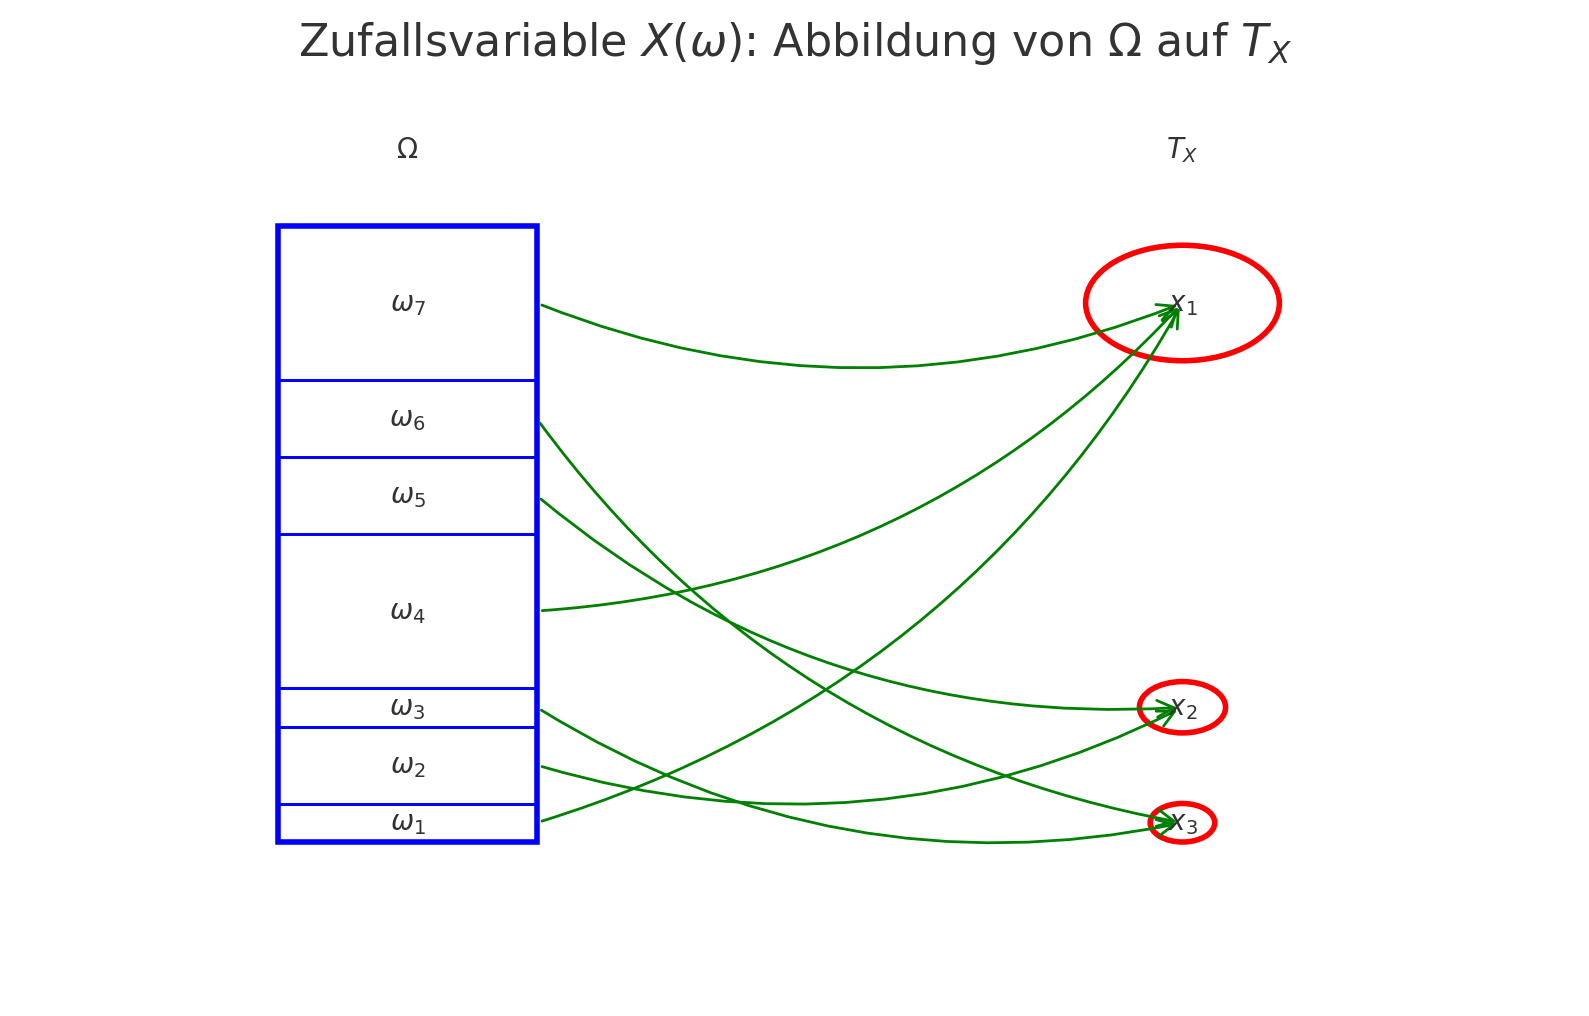
\includegraphics[height = 0.8\textheight]{pics/zv-diagramm.png}
\end{frame}

\begin{frame}{Zufallsvariable - Motivation}
\phantomsection\label{zufallsvariable---motivation}
\begin{itemize}
\item
  Man kann mit \(X\) ``rechnen'': z.B \(P(X \leq a)\) oder
  \(P(X^2 > b)\), oder ``Welches Ergebnis erwarten wir `im Mittel'?''
\item
  Ursprünglicher Wahrscheinlichkeitsraum \((\Omega, P)\) wird
  letztendlich nicht mehr benötigt, stattdessen nur Wahrscheinlichkeiten
  für die Werte der ZV\\
  \(\implies\) meist deutlich einfacher zu handhaben\\
  -- im Bsp: Verteilung über \(\{0,1,2,3\}\) statt über
  \(\{KKK, KKZ, KZK, ...., ZZK, ZZZ\}\)
\item
  Mathematische Formalisierung eines (quantitativen) Messvorgangs --
  jeder möglichen Beobachtung (= Elementarereignis) wird genau ein
  Zahlenwert zugeordnet.\\
  \(\longrightarrow\) in vielen Anwendungen \(\Omega\) kaum zugänglich
  oder mathematisch formalisierbar und nur Ergebnis des Messvorgangs
  überhaupt \emph{beobachtbar}\\
  \(\implies\) ZV zentraler Begriff für statistische Anwendungen und
  Ansatzpunkt für mathematische Formalisierung empirischer Phänomene
\end{itemize}
\end{frame}

\subsection{Diskrete Zufallsvariablen}\label{diskrete-zufallsvariablen}

\begin{frame}{Diskrete Zufallsvariable}
\phantomsection\label{diskrete-zufallsvariable}
\begin{block}{Def.: \textbf{Diskrete Zufallsvariable}}
\phantomsection\label{def.-diskrete-zufallsvariable}
Eine ZV \(X\) heißt \textbf{diskret}, falls sie nur endlich oder
abzählbar unendlich viele Werte \(x_1, x_2, ...\) annehmen kann, also:
falls die Menge \(\cal{T}=\{x_1, x_2, ...\}\) der möglichen Ausprägungen
\(x_i\) von \(X\) mit \(P(X = x_i)  > 0\) abzählbar ist.
\end{block}

\begin{block}{Def.: \textbf{Wahrscheinlichkeitsfunktion einer diskreten
ZV}}
\phantomsection\label{def.-wahrscheinlichkeitsfunktion-einer-diskreten-zv}
Die \emph{Wahrscheinlichkeitsfunktion} von \(X\) ist durch
\[f_X(x_i) := P(X = x_i) = P\left(\{\omega \in \Omega: X(\omega) = x_i\}\right)\]
für \(x_i \in \mathbb{R}\) gegeben.
\end{block}

\begin{itemize}
\tightlist
\item
  Alternativ: ``Wahrscheinlichkeitsdichte''
\end{itemize}

\note{Terminologie: Dichte, Dichtefunktion, density, pdf, pmf, abzählbar/überabzählbar}
\end{frame}

\begin{frame}{Folgerungen}
\phantomsection\label{folgerungen-1}
Als Funktion von \(B \subset \mathbb{R}\) ist also
\[P(X \in B) = P(\{\omega \in \Omega: X(\omega) \in B\})\] eine
Wahrscheinlichkeitsverteilung auf \(\mathbb{R}\).\\
Man nennt diese die \textbf{Verteilung} der Zufallsvariable \(X\).

Sie ist durch die Abbildung \(X\) und die Wahrscheinlichkeitsverteilung
\(P\) über \(\omega \in \Omega\) induziert. ~ ~

Für \(x \not \in {\cal{T}_X}\) ist \(f_X(x) = P(\emptyset) = 0\).
\end{frame}

\subsection{Verteilungsfunktion}\label{verteilungsfunktion}

\begin{frame}{Die Verteilungsfunktion}
\phantomsection\label{die-verteilungsfunktion}
\begin{block}{Def.: \textbf{Verteilungsfunktion} (diskret)}
\phantomsection\label{def.-verteilungsfunktion-diskret}
Die \emph{Verteilungsfunktion} einer diskreten ZV ist definiert als
\[F_X(x) := P(X \leq x) = \sum_{i: x_i \leq x} f_X(x_i).\]
\end{block}

Kennt man also die \textbf{Wahrscheinlichkeitsfunktion} \(f(x)\) für
alle \(x \in \cal{T}\), so kennt man auch die
\textbf{Verteilungsfunktion} \(F(x)\) und umgekehrt.

\note{Terminologie: cdf, cumulative density function, distribution (function)}
\end{frame}

\begin{frame}{Eigenschaften der Verteilungsfunktion}
\phantomsection\label{eigenschaften-der-verteilungsfunktion}
\begin{itemize}
\tightlist
\item
  \(F(x)\) ist monoton wachsend (``Treppenfunktion'')\\
\item
  \(F(x)\) ist stückweise konstant mit Sprungstellen an Werten \(x_i\)
  mit \(f(x_i) > 0\), d.h. an allen Realisierungen \(x_i \in {\cal{T}}\)
\item
  Die Höhe des Sprungs an der Stelle \(x_i \in {\cal{T}}\) ist
  \(f(x_i)\)
\item
  \(\lim\limits_{x \to \infty} F(x) = 1\)
\item
  \(\lim\limits_{x \to -\infty} F(x) = 0\)
\end{itemize}
\end{frame}

\begin{frame}{Beispiel: 3-maliger Münzwurf}
\phantomsection\label{beispiel-3-maliger-muxfcnzwurf}
\(X :=\) ``Anzahl Kopf'', \({\cal{T}}=\{0,1,2,3\}\)

\[\begin{array}{lll}
f(0) &= P(\{ZZZ\}) &= 1/8\\
f(1) &= P(\{KZZ, ZKZ, ZZK\}) &= 3/8\\
f(2) &= P(\{KKZ, KZK, ZKK\}) &= 3/8\\
f(3) &= P(\{KKK\}) &= 1/8\\
\end{array}
\qquad
\implies
\qquad
F(x) = \begin{cases}
0 & x < 0 \\
1/8 & 0 \leq x < 1\\
4/8 & 1 \leq x < 2\\
7/8 & 2 \leq x < 3\\
1 & x \geq 3
\end{cases}\]

Beachte: \(f(x)=0\) für alle \(x \notin {\cal{T}}\)
\end{frame}

\subsection{Stetige Zufallsvariablen}\label{stetige-zufallsvariablen}

\begin{frame}{Stetige Zufallsvariable - Definition 1}
\phantomsection\label{stetige-zufallsvariable---definition-1}
\begin{block}{Def.: \textbf{Stetige Zufallsvariable}}
\phantomsection\label{def.-stetige-zufallsvariable}
Eine Zufallsvariable \(X\) ist \textbf{stetig}, falls ihr Träger eine
\emph{überabzählbare} Teilmenge der reellen Zahlen \(\mathbb{R}\) ist.\\
\end{block}

~

\emph{Beispiel:}\\
Glücksrad mit stetigem Wertebereich \([0°, 360°)\)\\
Von Interesse also die Zufallsvariable, die den \emph{exakten} Winkel
angibt, an dem das Glücksrad stehen bleibt.
\end{frame}

\begin{frame}{Stetige Zufallsvariablen - Definition 2}
\phantomsection\label{stetige-zufallsvariablen---definition-2}
\begin{block}{Def.: \textbf{Stetige Zufallsvariable}}
\phantomsection\label{def.-stetige-zufallsvariable-1}
Eine Zufallsvariable \(X\) heißt \emph{stetig}, wenn es eine Funktion
\(f(x) \geq 0\) gibt, so dass sich die Verteilungsfunktion
\(F_X(x) := P(X \leq x)\) von \(X\) wie folgt darstellen lässt:
\[F_X(x) = \int_{-\infty}^x f_X(u) du\]
\end{block}

\begin{block}{Def.: \textbf{Dichtefunktion einer (stetigen) ZV}}
\phantomsection\label{def.-dichtefunktion-einer-stetigen-zv}
Diese nicht-negative Funktion \(f(x)\) zur Verteilungsfunktion \(F(x)\)
heißt \emph{Wahrscheinlichkeitsdichte} (auch: \emph{Dichte} oder
\emph{Dichtefunktion}) von \(X\).
\end{block}

\hfill\break

Beachte: bei \emph{diskreten} Zufallsvariablen gilt
\(F(x) = \sum_{i: x_i \leq x} f(x_i)\).
\end{frame}

\begin{frame}[fragile]{Folgerungen}
\phantomsection\label{folgerungen-2}
\begin{itemize}
\item
  \(\int_{-\infty}^{+\infty} f(x)\,dx = 1\)\\
  \strut ~
\item
  Mit Dichte- bzw. Verteilungsfunktion lassen sich W.keiten für
  beliebige Teilmengen des Trägers ausrechnen:\\
  \(P(X \in [a, b])  =  \int_a^b f(x)\,dx = F(b) - F(a)\)\\
  \strut ~
\item
  Unintuitive Konsequenz:\\
  für stetige ZV \(X\) gilt
  \(P(X = x) = 0 \; \forall \; x \in \mathbb{R}\)!

  \scriptsize \href{https://youtu.be/ZA4JkHKZM50}{Video dazu von
  \texttt{3blue1brown}}
\end{itemize}
\end{frame}

\begin{frame}{Folgerungen}
\phantomsection\label{folgerungen-3}
\begin{itemize}
\item
  \(\lim\limits_{x \to -\infty} F(x) = 0\)
\item
  \(\lim\limits_{x \to \infty} F(x) = 1\)
\item
  \(F'(x) = f(x)\) überall dort wo \(f(x)\) stetig ist.
\item
  \(P(a \leq X \leq b) = F(b) - F(a)\)
\item
  \(P(X > a) = 1 - F(a)\)
\end{itemize}
\end{frame}

\begin{frame}{Ausblick}
\phantomsection\label{ausblick}
Stringentere Definitionen in späteren Vorlesungen zu W.keitstheorie ~

Eine allgemein gültige Definition ohne Fallunterscheidungen zwischen

\begin{itemize}
\tightlist
\item
  diskreten ZVn,
\item
  stetigen ZVn,
\item
  und ZVn, deren Träger teils stetig und teils diskret ist,
\end{itemize}

benötigt Maßtheorie mit einem verallgemeinertem Integrationsbegriff.
\end{frame}

\subsection{Empirische
Häufigkeitsverteilungen}\label{empirische-huxe4ufigkeitsverteilungen}

\begin{frame}{Empirische Häufigkeitsverteilungen}
\end{frame}

\begin{frame}{Zurück zur Empirie}
\phantomsection\label{zuruxfcck-zur-empirie}
Zufallsvariablen sind Bestandteil der mathematischen Formalisierung
eines zufälligen Prozesses.

Jetzt: Betrachte \emph{empirische} Entsprechungen der eben eingeführten
Begriffe.
\end{frame}

\begin{frame}{Häufigkeitsverteilung: Notation \& Terminologie}
\phantomsection\label{huxe4ufigkeitsverteilung-notation-terminologie}
Im Weiteren:

\begin{itemize}
\tightlist
\item
  \(X, Y, \ldots\) Bezeichnung für \textbf{Merkmale}
\item
  \(n\) ist Anzahl der \textbf{Untersuchungseinheiten}
\item
  \(x_i, i \in \{1, \ldots, n\}\) ist \textbf{beobachteter Wert} bzw.
  \textbf{Merkmalsausprägung} von Merkmal \(X\) für \(i\)-te
  Untersuchungseinheit
\item
  \(x_1, \ldots, x_n\) \textbf{Rohdaten}, \textbf{Urliste}
\item
  \(a_1, a_2, \ldots, a_k, \, k \le n\) (evtl. der Größe nach geordnete)
  \emph{verschiedene} Werte der Urliste \(x_1,\ldots,x_n\): die
  \textbf{Menge der beobachteten Merkmalsausprägungen} von \(X\).
\end{itemize}
\end{frame}

\begin{frame}{Eindimensionale Häufigkeitsverteilung}
\phantomsection\label{eindimensionale-huxe4ufigkeitsverteilung}
\begin{itemize}
\tightlist
\item
  Sortierung der Daten nach einem Merkmal
\item
  Auszählen der Häufigkeiten der einzelnen Merkmalsausprägungen
\item
  \textbf{Relative Häufigkeiten} = Häufigkeit einer Merkmalsausprägung /
  Anzahl der Untersuchungseinheiten (\emph{Anteil})
\item
  \textbf{Kumulative relative Häufigkeiten} bei ordinal oder metrisch
  skalierten Merkmalen sinnvoll:\\
  \(F(x):=\) ``Anteil UE mit Merkmalsausprägung \(\leq x\)'' heißt
  \textbf{empirische Verteilungsfunktion}
\end{itemize}
\end{frame}

\begin{frame}{Häufigkeitsverteilungen}
\phantomsection\label{huxe4ufigkeitsverteilungen}
\textbf{Bemerkungen:}

\begin{itemize}
\tightlist
\item
  Für Nominalskalen hat die Anordnung ``\(<\)'' keine inhaltliche
  Bedeutung.
\item
  Bei kategorialen Merkmalen \(k =\) Anzahl der Kategorien\\
\item
  Bei stetigen Merkmalen \(k\) oft nicht oder kaum kleiner als \(n\).
\end{itemize}
\end{frame}

\begin{frame}{Absolute und relative Häufigkeiten}
\phantomsection\label{absolute-und-relative-huxe4ufigkeiten}
\begin{tabular}{ll}
$h(a_j) = h_j$ & \textbf{absolute Häufigkeit} der
Ausprägung $a_j$,\\*[0.7cm]
           &  d.h.~Anzahl der $x_i$ aus $x_1,\dots x_n$ mit $x_i = a_j$
\\*[0.7cm]
$ f(a_j) = f_j = h_j/n$ & \textbf{relative Häufigkeit}
von $a_j$ \\*[0.7cm]
$h_1 , \ldots , h_k$    & \textbf{absolute
Häufigkeitsverteilung} \\*[0.7cm]
$f_1 , \ldots , f_k $   & \textbf{relative
Häufigkeitsverteilung}
\end{tabular}
\end{frame}

\begin{frame}{Bemerkungen:}
\phantomsection\label{bemerkungen}
\begin{itemize}
\tightlist
\item
  Wenn statt der Urliste bereits die Ausprägungen \(a_1,\ldots,a_k\) und
  ihre Häufigkeiten \(f_1,\ldots,f_k\) bzw. \(h_1,\ldots,h_k\)
  vorliegen, sprechen wir von \textbf{Häufigkeitsdaten}.
\item
  \textbf{Klassenbildung}, \textbf{gruppierte Daten}: Vor allem bei
  metrischen, stetigen (oder quasi-stetigen) Merkmalen oft Aggregation
  der Urliste durch Bildung geeigneter Klassen
\end{itemize}
\end{frame}

\begin{frame}[fragile]{Beispiel Nettomieten I}
\phantomsection\label{beispiel-nettomieten-i}
\scriptsize\normalsize

Wir greifen aus dem gesamten Datensatz des Münchner Mietspiegels 2015
die Wohnungen ohne zentrale Warmwasserversorgung (\texttt{zh0\ ==\ 1})
und mit einer Wohnfläche kleiner als \(60m^2\)
(\texttt{wfl\ \textless{}\ 60}) heraus.

Die folgende Urliste zeigt, bereits der Größe nach geordnet, die
Nettomieten dieser \(n=88\) Wohnungen:

\scriptsize

\begin{Shaded}
\begin{Highlighting}[]
\NormalTok{mietspiegel\_url }\OtherTok{\textless{}{-}} \StringTok{"http://chris.userweb.mwn.de/statistikbuch/mietspiegel2015.txt"}
\NormalTok{mietspiegel }\OtherTok{\textless{}{-}} \FunctionTok{read.table}\NormalTok{(}\AttributeTok{file =}\NormalTok{ mietspiegel\_url, }\AttributeTok{header =} \ConstantTok{TRUE}\NormalTok{)}
\NormalTok{klein\_und\_kalt }\OtherTok{\textless{}{-}} \FunctionTok{subset}\NormalTok{(mietspiegel, zh0 }\SpecialCharTok{==} \DecValTok{1} \SpecialCharTok{\&}\NormalTok{ wfl }\SpecialCharTok{\textless{}} \DecValTok{60}\NormalTok{)}
\FunctionTok{sort}\NormalTok{(klein\_und\_kalt[, }\StringTok{"nm"}\NormalTok{]) }\SpecialCharTok{|\textgreater{}}
    \FunctionTok{print}\NormalTok{(}\AttributeTok{digits =} \DecValTok{4}\NormalTok{)}
\end{Highlighting}
\end{Shaded}

\begin{verbatim}
##  [1] 174.8 175.0 211.0 211.9 212.9 245.0 257.2 266.8 276.6 278.1 282.4 287.4
## [13] 294.9 299.5 302.9 308.4 315.7 318.0 322.0 323.0 330.0 336.0 336.0 338.5
## [25] 339.7 343.0 346.5 362.0 363.5 370.0 375.1 379.6 380.0 390.4 391.4 395.1
## [37] 408.9 410.0 415.6 421.8 437.7 440.0 440.0 443.6 446.6 451.6 452.2 461.9
## [49] 470.0 472.4 480.8 490.0 495.0 500.0 510.0 513.0 515.0 515.0 517.1 518.0
## [61] 520.2 521.6 523.0 526.5 540.0 543.0 550.0 551.0 556.0 570.0 570.0 573.5
## [73] 576.0 590.0 590.0 590.0 600.7 610.0 610.0 630.0 638.0 660.0 695.0 700.0
## [85] 700.0 726.9 730.0 790.0
\end{verbatim}

\normalsize

Alle Werte verschieden:\\
\(\Rightarrow k=n\) und
\(\{x_1 , \ldots , x_n\} = \{a_1 , \ldots , a_k\};\; f_j = \frac{1}{88} \,\forall\,  j = 1, \ldots, 88\).
\end{frame}

\begin{frame}[fragile]{Beispiel Nettomieten II}
\phantomsection\label{beispiel-nettomieten-ii}
Gruppiert man die Urliste in \(7\) Klassen mit gleicher Klassenbreite
von \(100\)€, so erhält man folgende Häufigkeitstabelle:

\scriptsize

\begin{Shaded}
\begin{Highlighting}[]
\NormalTok{gruppierung }\OtherTok{\textless{}{-}} \FunctionTok{seq}\NormalTok{(}\AttributeTok{from =} \DecValTok{150}\NormalTok{, }\AttributeTok{to =} \DecValTok{850}\NormalTok{, }\AttributeTok{by =} \DecValTok{100}\NormalTok{)}
\NormalTok{klein\_und\_kalt[, }\StringTok{"nm\_gruppiert"}\NormalTok{] }\OtherTok{\textless{}{-}} \FunctionTok{cut}\NormalTok{(klein\_und\_kalt[, }\StringTok{"nm"}\NormalTok{], }\AttributeTok{breaks =}\NormalTok{ gruppierung)}
\FunctionTok{table}\NormalTok{(klein\_und\_kalt[, }\StringTok{"nm\_gruppiert"}\NormalTok{])}
\end{Highlighting}
\end{Shaded}

\begin{verbatim}
## 
## (150,250] (250,350] (350,450] (450,550] (550,650] (650,750] (750,850] 
##         6        21        18        22        14         6         1
\end{verbatim}

\normalsize

\normalsize

\begin{table}[ht]
\centering
\begin{tabular}{rrrr}
 Klasse & absolute H.keit & relative H.keit & kumulative rel. H.keit \\ 
  \hline
(150,250] &   6 & 0.07 & 0.07 \\ 
  (250,350] &  21 & 0.24 & 0.31 \\ 
  (350,450] &  18 & 0.20 & 0.51 \\ 
  (450,550] &  22 & 0.25 & 0.76 \\ 
  (550,650] &  14 & 0.16 & 0.92 \\ 
  (650,750] &   6 & 0.07 & 0.99 \\ 
  (750,850] &   1 & 0.01 & 1.00 \\ 
  \end{tabular}
\end{table}
\normalsize
\end{frame}

\subsection{Empirische
Verteilungsfunktion}\label{empirische-verteilungsfunktion}

\begin{frame}{Empirische Verteilungsfunktion}
\phantomsection\label{empirische-verteilungsfunktion-1}
Häufigkeitsfunktion: \[H(x) := (\mbox{Anzahl der Werte} \leq x)  \]

Verteilungsfunktion: \[
F_n(x)  =  H(x)/n = (\mbox{Anteil der Werte}\,\,\, x_i \,\,\, \mbox{mit} \,\,\, x_i
\leq x)
\] bzw. \[
F_n(x) =  f(a_1) + \ldots + f(a_j) = \sum_{i: a_i \leq x} f_i,
\] für \(a_j \leq x\) und \(a_{j+1}>x\).

\scriptsize **ECDF** (empirical cumulative distribution function)
\end{frame}

\begin{frame}{Eigenschaften der ECDF \(F_n(x)\)}
\phantomsection\label{eigenschaften-der-ecdf-f_nx}
\begin{itemize}
\tightlist
\item
  monoton wachsende Treppenfunktionen mit Sprüngen an den Ausprägungen
  \(a_1, \ldots, a_k\)
\item
  Sprunghöhen: \(f_1, \ldots, f_k\)
\item
  rechtsseitig stetig
\item
  \(F_n(x) = 0\) für \(x < a_1, \,\,F_n(x) = 1\) für \(x \geq a_k\)
\end{itemize}
\end{frame}

\begin{frame}{Beispiel: \(F_n\)(Quadratmetermiete) für Klein \& Kalt}
\phantomsection\label{beispiel-f_nquadratmetermiete-fuxfcr-klein-kalt}
\scriptsize

\begin{center}\includegraphics[width=.9\textwidth,height=.8\textheight]{main_files/figure-beamer/02-ecdf-1} \end{center}

\normalsize
\end{frame}

\begin{frame}{Beispiel: \(F_n\)(Quadratmetermiete) für Klein \& Kalt}
\phantomsection\label{beispiel-f_nquadratmetermiete-fuxfcr-klein-kalt-1}
Wie groß ist der Anteil von kleinen Wohnungen ohne ZH mit qm-Miete
\(\leq\) 12 €? Wie viel kosten die günstigsten 25\% der Wohnungen
höchstens?

\scriptsize

\begin{center}\includegraphics[width=.9\textwidth,height=.7\textheight]{main_files/figure-beamer/02-ecdf-ex-q-1} \end{center}

\normalsize
\end{frame}

\begin{frame}{Beispiel: \(F_n\)(Quadratmetermiete) für Klein \& Kalt}
\phantomsection\label{beispiel-f_nquadratmetermiete-fuxfcr-klein-kalt-2}
Wie groß ist der Anteil von kleinen Wohnungen ohne ZH mit qm-Miete
\(\leq\) 12 €?

\scriptsize

\begin{center}\includegraphics[width=.9\textwidth,height=.7\textheight]{main_files/figure-beamer/02-ecdf-ex-a1-1} \end{center}

\normalsize

\(\Rightarrow \approx\) 80\%
\end{frame}

\begin{frame}{Beispiel: \(F_n\)(Quadratmetermiete) für Klein \& Kalt}
\phantomsection\label{beispiel-f_nquadratmetermiete-fuxfcr-klein-kalt-3}
Wie viel kosten die günstigsten 25\% der Wohnungen höchstens?\\
Was ist die maximale qm-Miete im billigsten unteren Viertel der
Wohnungen?

\scriptsize

\begin{center}\includegraphics[width=.9\textwidth,height=.7\textheight]{main_files/figure-beamer/02-ecdf-ex-a2-1} \end{center}

\normalsize

\(\Rightarrow \approx\) 7.3€
\end{frame}

\begin{frame}{Theorie \& Empirie}
\phantomsection\label{theorie-empirie-4}
\begin{longtable}[]{@{}
  >{\raggedright\arraybackslash}p{(\columnwidth - 4\tabcolsep) * \real{0.4444}}
  >{\raggedright\arraybackslash}p{(\columnwidth - 4\tabcolsep) * \real{0.1111}}
  >{\raggedright\arraybackslash}p{(\columnwidth - 4\tabcolsep) * \real{0.4444}}@{}}
\toprule\noalign{}
\begin{minipage}[b]{\linewidth}\raggedright
Theorie
\end{minipage} & \begin{minipage}[b]{\linewidth}\raggedright
\end{minipage} & \begin{minipage}[b]{\linewidth}\raggedright
Empirie
\end{minipage} \\
\midrule\noalign{}
\endhead
Zufallsvariable \(X\) & \(\cong\) & Merkmal \(X\) \\
Träger \(T_X\) & \(\supseteq\) & Beobachtete Merkmalsausprägungen
\(\{a_1, \dots, a_k\}\) von \(X\) \\
W.keitsfunktion \(f_X(x)\) & \(\leftrightarrow\) & relative H.keiten
\(f_X(a_j)\) \\
Verteilungsfunktion \(F_X(x)\) & \(\leftrightarrow\) & kumul. relative
H.keiten / empirische Verteilungsfunktion \(F_n(x)\) \\
\bottomrule\noalign{}
\end{longtable}
\end{frame}

\section{Statistische Grafiken}\label{statistische-grafiken}

\subsection{Grammar of Graphics}\label{grammar-of-graphics}

\begin{frame}[fragile]{Statistische Grafik}
\phantomsection\label{statistische-grafik}
Statistische Grafiken\\
repräsentieren die \emph{Ausprägungen} gewisser \emph{Merkmale} in einem
\emph{Datensatz}\\
durch die \emph{ästhetischen} Eigenschaften \emph{geometrischer}
Objekte.

Aus dieser Definition können wir eine formale ``Grammatik'' für
grafische Darstellungen ableiten.

\footnotesize

(s.a. Wilkinson (2005) \emph{The Grammar of Graphics},\\
Wickham et al.~(2020)
\href{https://ggplot2-book.org/}{\emph{\texttt{ggplot2}: Elegant
Graphics for Data Analysis}})
\end{frame}

\begin{frame}{Grammar of Graphics}
\phantomsection\label{grammar-of-graphics-1}
(Fast) jede sinnvolle Grafik lässt sich als Kombination der folgenden
Basis-Elemente beschreiben:

\begin{itemize}
\tightlist
\item
  \emph{Daten}: enthalten die \emph{Beobachtungen} der dargestellten
  \emph{Merkmale}\\
  (Oft auch: daraus abgeleitete \emph{Statistiken} wie Anteile,
  Mittelwerte, etc)\\
\item
  \emph{Geometrische Elemente}: z.B. Punkte, Linien, Rechtecke,
  etc\ldots{}
\item
  \emph{Ästhetische Zuordnungen}: die \emph{Ausprägungen} der in der
  Grafik dargestellten \emph{Merkmale} werden durch sichtbare
  Eigenschaften der geometrischen Elemente repräsentiert, z.B.

  \begin{itemize}
  \tightlist
  \item
    Position (vertikal/horizontal)
  \item
    Farbe
  \item
    Größe
  \item
    Form
  \end{itemize}
\end{itemize}
\end{frame}

\begin{frame}{Grammar of Graphics}
\phantomsection\label{grammar-of-graphics-2}
Also: \emph{Daten} werden über \emph{ästhetische Eigenschaften} von
\emph{geometrischen Elementen} dargestellt.

zusätzlich:

\begin{itemize}
\tightlist
\item
  \emph{Datentransformationen}/\emph{Statistiken}: Oft werden nicht
  Rohdaten selbst, sondern daraus abgeleitet Größen (Mittelwerte,
  Anteile, \ldots.) abgebildet. Komplexere geometrische Elemente
  basieren oft intern auf Datentransformationen (\(\rightarrow\)
  Balkendiagramme, geglättete Trendlinien, Boxplots, \ldots.).
\item
  \emph{Skalen} ordnen für ein gegebenes \emph{Merkmal}/\emph{Statistik}
  und ihrer \emph{ästhetischen Zuordnung} jeder \emph{Ausprägungen}
  bestimmte Werte zu (z.B. Achsenabschnitte für Position, Farbpaletten
  für Farbe, etc\ldots) und legen damit auch Legenden (z.B. für
  Farbskalen) und Achsenbeschriftungen fest.
\item
  \emph{Koordinatensysteme}: kartesische / logarithmische /
  Polarkoordinatensysteme; Kartenprojektionen
\end{itemize}
\end{frame}

\begin{frame}[fragile]{Grammar of Graphics}
\phantomsection\label{grammar-of-graphics-3}
zusätzlich:

\begin{itemize}
\tightlist
\item
  \emph{Facettierung} definiert anhand welcher Merkmale die Daten in
  Subgruppen aufgeteilt werden und wie die Darstellungen der
  verschiedenen Subgruppen arrangiert werden (s.a.: \emph{small
  multiples} plot, \emph{lattice} plots).
\item
  \emph{Theme}: umfasst sämtliche Designaspekte wie Fonteigenschaften,
  Gitterlinien, Hintergrundfarben, Layout von Textelementen und
  Legenden, \ldots{}
\end{itemize}

Implementation in R: \texttt{ggplot2}\\
Python: \texttt{plotnine}
\end{frame}

\begin{frame}{Beispiele: Geometrien}
\phantomsection\label{beispiele-geometrien}
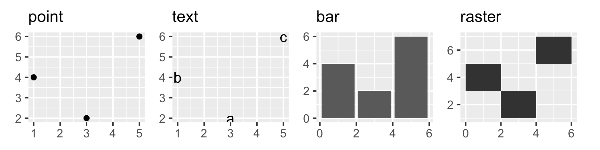
\includegraphics{pics/02-geoms1.png}

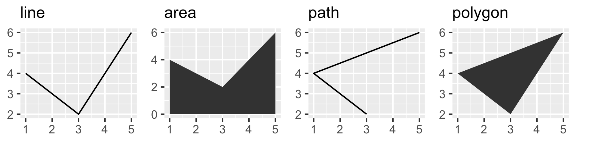
\includegraphics{pics/02-geoms2.png}

.. und viele viele mehr \ldots{}

\footnotesize

Abb: Wickham et al.~(2020)
\end{frame}

\begin{frame}{Beispiele: Ästhetiken}
\phantomsection\label{beispiele-uxe4sthetiken}
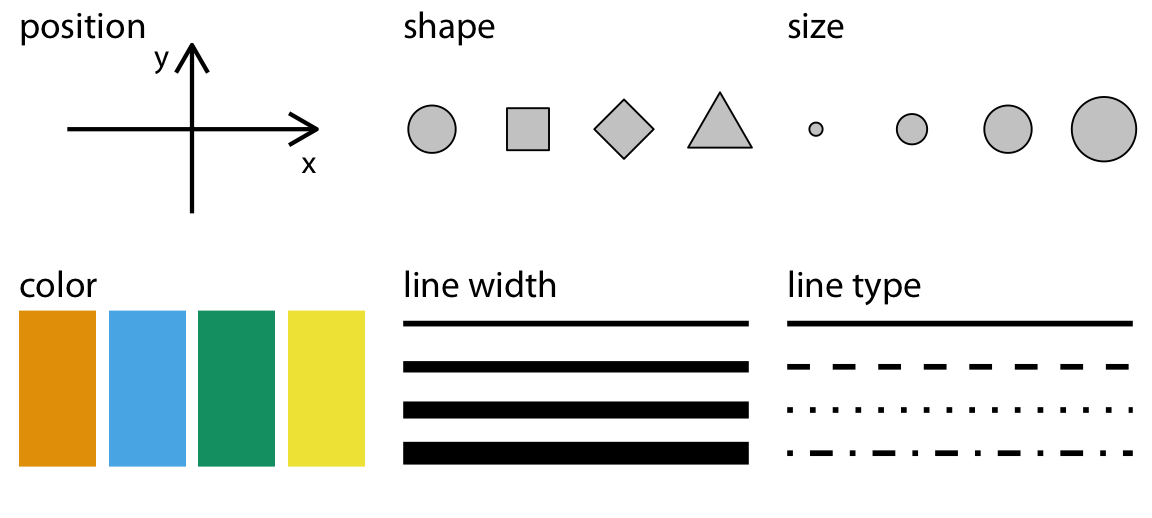
\includegraphics{pics/02-aesthetics.png}\\
\footnotesize Abb:
\href{https://clauswilke.com/dataviz/aesthetic_mapping_files/figure-html/common-aesthetics-1.png}{Wilke
(2020)}
\end{frame}

\begin{frame}{Grammar of Graphics: Beispiele mit Code}
\phantomsection\label{grammar-of-graphics-beispiele-mit-code}
\href{https://pkg.garrickadenbuie.com/gentle-ggplot2/\#68}{Aden-Buie,
2018}

\href{https://evamaerey.github.io/ggplot2_grammar_guide/ggplot2_grammar_guide.html\#30}{Reynolds,
2019}
\end{frame}

\subsection{Grafiken: Wahrnehmung}\label{grafiken-wahrnehmung}

\begin{frame}{Wahrnehmung von Grafiken}
\phantomsection\label{wahrnehmung-von-grafiken}
Wahrnehmungspsychologische Experimente zeigen deutliche Unterschiede in
der korrekten Interpretation der folgenden Grafiktypen:

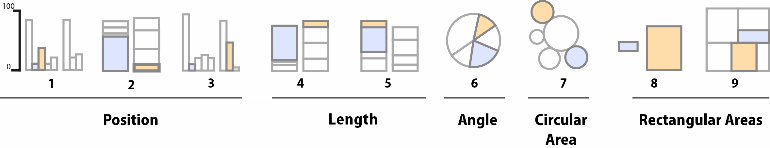
\includegraphics{pics/02-clevelandgill1.png}

\scriptsize

Abb.: Healy, K. (2018). \href{https://socviz.co}{Data visualization: a
practical introduction}. Princeton University Press. (übernommen aus
\href{http://vis.stanford.edu/files/2010-MTurk-CHI.pdf}{Heer \&
Bostock})

\textbackslash vskip 3em Cleveland, W.S., Mc3Gill, R. (1984):
\href{http://www.math.pku.edu.cn/teachers/xirb/Courses/biostatistics/Biostatistics2016/GraphicalPerception_Jasa1984.pdf}{Graphical
Perception: Theory, Experimentation, and Application to the Development
of Graphical Methods.} \emph{JASA} 79(387), 531--554.\\
Heer, J., Bostock, M. (2010):
\href{http://vis.stanford.edu/files/2010-MTurk-CHI.pdf}{Crowdsourcing
graphical perception: using Mechanical Turk to assess visualization
design.} \emph{SIGCHI Proceedings}, 203--212.
\end{frame}

\begin{frame}{Wahrnehmung von Grafiken}
\phantomsection\label{wahrnehmung-von-grafiken-1}
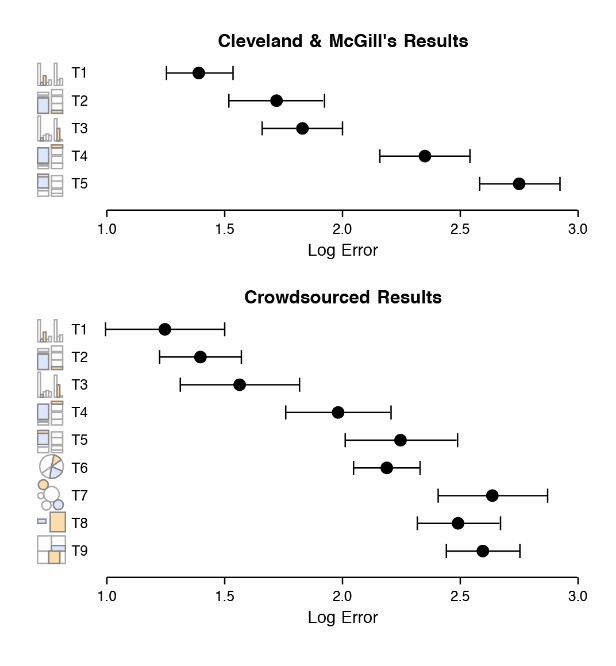
\includegraphics{pics/02-clevelandgill2.png}
\end{frame}

\begin{frame}{Wahrnehmung von Grafiken}
\phantomsection\label{wahrnehmung-von-grafiken-2}
Hierarchie der korrekten Interpretation:

\begin{enumerate}
\tightlist
\item
  Position (gemeinsame/parallele Skala \(>\) verschobene Skalen)\\
\item
  Abstände \& Längen
\item
  Steigung \& Winkel
\item
  Flächen
\item
  Volumen
\item
  Farbton-Farbsättigung-Farbhelligkeit
\end{enumerate}

Da \textbf{Position \& Abstände} am besten wahrgenommen werden, müssen
diese verwendet werden um die wichtigsten Merkmale zu codieren.
\end{frame}

\begin{frame}{\emph{Principles of Graphical Excellence}}
\phantomsection\label{principles-of-graphical-excellence}
\begin{itemize}
\tightlist
\item
  Graphical excellence is the well-designed presentation of interesting
  data -- a matter of \emph{substance}, of \emph{statistics} and of
  \emph{design}.
\item
  Graphical excellence consists of complex ideas communicated with
  \emph{clarity, precision and efficiency}.
\item
  Graphical excellence is that which gives to the viewer the
  \emph{greatest number of ideas} in the \emph{shortest time} with the
  \emph{least ink} in the \emph{smallest space}.
\item
  Graphical excellence is nearly always \emph{multivariate}.
\item
  And graphical excellence requires telling the \emph{truth about the
  data}.
\end{itemize}

\scriptsize

Tufte, E. (2001): \emph{The Visual Display of Information.} Graphic
Press 2nd ed.
\end{frame}

\begin{frame}{Goldene Regeln für Grafikgestaltung}
\phantomsection\label{goldene-regeln-fuxfcr-grafikgestaltung}
\begin{itemize}
\tightlist
\item
  Verständnis von Grafiken erfordert:

  \begin{itemize}
  \tightlist
  \item
    \emph{Detektion}: Erkennen welche geometrischen Elemente und
    ästhetische Eigenschaften welche Werte repräsentieren
  \item
    \emph{Synthese}: Gruppierung \& In-Relation-Setzen der entdeckten
    Inhalte
  \item
    \emph{Evaluation}: Bewertung der relativen Größen und Bedeutung
    dieser Inhalte.\\
    Speziell: Unterscheidung, Rangbildung, Abschätzung von
    Verhältnissen.
  \end{itemize}
\item
  alle drei Phasen unterstützt durch \emph{bewusste Wahl}

  \begin{itemize}
  \tightlist
  \item
    geeigneter Ästhetiken \& Geometrien (s.o.: Abstände \(>\) Farbe,
    etc.)
  \item
    geeigneter Achsen, Gitterlinien und Seitenverhältnisse
  \item
    inhaltlich adäquater Sortierung/Reihenfolge der Ausprägungen
    qualitativer Merkmale
  \item
    entsprechender Annotationen \& Hervorhebungen
  \end{itemize}
\end{itemize}

\(\implies\) \textbf{Kommunikationsabsicht} klarmachen:\\
Welche Informationen will ich primär vermitteln? Welche zusätzlich? Auf
welche Vergleiche soll Aufmerksamkeit gelenkt werden?

\(\implies\) \textbf{Lesbarkeit} maximieren -- sowohl Genauigkeit als
auch Geschwindigkeit/Schwierigkeit sind wichtig.

\scriptsize

Harrell, F.E. (2017),
\href{https://hbiostat.org/doc/graphscourse.pdf}{Principles of Graph
Construction};\\
Grolemund, G., Wickham, H. (2017)
\href{https://r4ds.had.co.nz/graphics-for-communication.html}{R for Data
Science, Ch. 28}; Rauser, J. (2016)
\href{https://www.youtube.com/watch?v=fSgEeI2Xpdc}{How Humans See Data}
\end{frame}

\subsection{Grafiken: Infoviz vs Statistische
Grafiken}\label{grafiken-infoviz-vs-statistische-grafiken}

\begin{frame}{``Infoviz'' vs Statistische Grafiken I}
\phantomsection\label{infoviz-vs-statistische-grafiken-i}
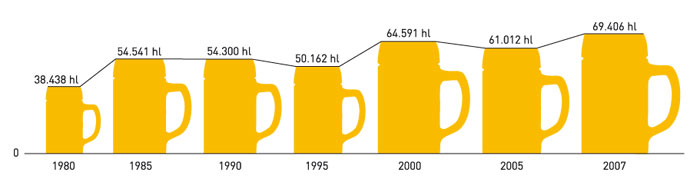
\includegraphics[width = \textwidth]{pics/2-bier.jpg}
\end{frame}

\begin{frame}{``Infoviz'' vs Statistische Grafiken I}
\phantomsection\label{infoviz-vs-statistische-grafiken-i-1}
\scriptsize

\begin{center}\includegraphics[width=.9\textwidth,height=.8\textheight]{main_files/figure-beamer/bier-1} \end{center}

\normalsize
\end{frame}

\begin{frame}{``Infoviz'' vs Statistische Grafiken I}
\phantomsection\label{infoviz-vs-statistische-grafiken-i-2}
\scriptsize

\begin{center}\includegraphics[width=.9\textwidth,height=.8\textheight]{main_files/figure-beamer/bier2-1} \end{center}

\normalsize
\end{frame}

\begin{frame}{``Infoviz'' vs Statistische Grafiken II}
\phantomsection\label{infoviz-vs-statistische-grafiken-ii}
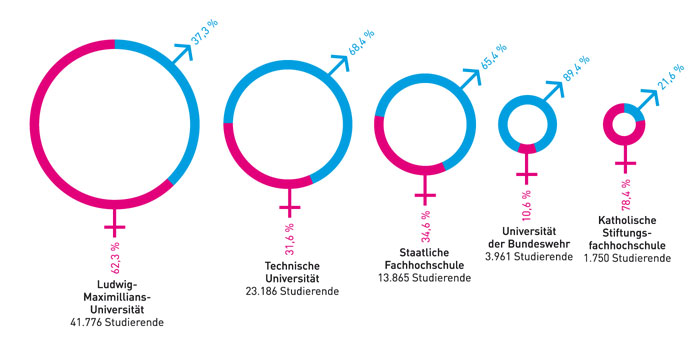
\includegraphics[width = \textwidth]{pics/2-studenten.jpg}
\end{frame}

\begin{frame}{``Infoviz'' vs Statistische Grafiken II}
\phantomsection\label{infoviz-vs-statistische-grafiken-ii-1}
\scriptsize

\begin{center}\includegraphics[width=.9\textwidth,height=.8\textheight]{main_files/figure-beamer/studis-1} \end{center}

\normalsize
\end{frame}

\begin{frame}{``Infoviz'' vs Statistische Grafiken II}
\phantomsection\label{infoviz-vs-statistische-grafiken-ii-2}
\scriptsize

\begin{center}\includegraphics[width=.9\textwidth,height=.8\textheight]{main_files/figure-beamer/studis2-1} \end{center}

\normalsize
\end{frame}

\begin{frame}{``Infoviz'' vs Statistische Grafiken IV}
\phantomsection\label{infoviz-vs-statistische-grafiken-iv}
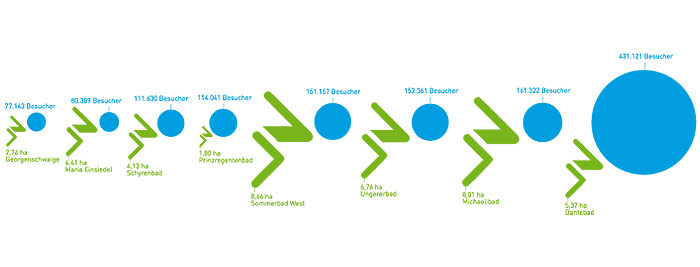
\includegraphics[width = \textwidth]{pics/2-freibad.jpg}
\end{frame}

\begin{frame}{``Infoviz'' vs Statistische Grafiken IV}
\phantomsection\label{infoviz-vs-statistische-grafiken-iv-1}
\scriptsize

\begin{center}\includegraphics[width=.9\textwidth,height=.8\textheight]{main_files/figure-beamer/freibad-1} \end{center}

\normalsize

\scriptsize\normalsize
\end{frame}

\subsection{Farbskalen}\label{farbskalen}

\begin{frame}{Wahrnehmung Ästhetischer Zuordnungen}
\phantomsection\label{wahrnehmung-uxe4sthetischer-zuordnungen}
Kodieren von Information durch:

\begin{itemize}
\tightlist
\item
  \textbf{Position, Längen \& Abstände}: am einfachsten zu erkennen,
  v.a. für gemeinsame/parallele Skalen
\item
  \textbf{Winkel \& Steigung}: visueller Eindruck abhängig von Richtung
  \& vom Seitenverhältnis der Darstellung
\item
  \textbf{Flächen}:

  \begin{itemize}
  \tightlist
  \item
    lang/dünn erscheint größer als kompakt/konvex
  \item
    abhängig von Farbe: hellere Flächen wirken größer
  \end{itemize}
\item
  \textbf{Farbe}: oft schwierig präzise Vergleiche abzulesen

  \begin{itemize}
  \tightlist
  \item
    dennoch allgegenwärtig da \emph{kombinierbar} mit anderen grafischen
    Elementen.
  \end{itemize}
\end{itemize}
\end{frame}

\begin{frame}{Farbwahrnehmung}
\phantomsection\label{farbwahrnehmung}
\begin{itemize}
\tightlist
\item
  Farbwahrnehmung ist komplex
\item
  Farben für Grafiken so wählen dass
  \textbf{Wahrnehmungseinheitlichkeit} berücksichtigt wird:

  \begin{itemize}
  \tightlist
  \item
    Grün-/Gelbtöne werden bei gleicher Sättigung intensiver wahrgenommen
    als andere Farben
  \item
    Sehschwächen mitbedenken
  \end{itemize}
\end{itemize}
\end{frame}

\begin{frame}{Farbwahrnehmung}
\phantomsection\label{farbwahrnehmung-1}
Rot-Grün-Sehschwäche\\
(Protanopia: Prävalenz 6\%, Deuteranopia: Prävalenz 2\%)

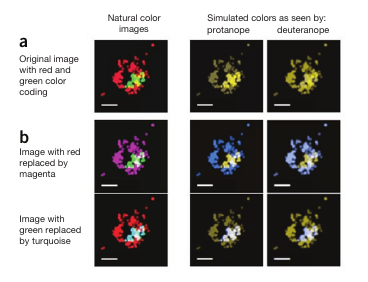
\includegraphics[height=.7\textheight]{pics/5-colorblind.png}

\begin{scriptsize} 
aus  Wong, B. \textit{Nature Methods} \textbf{8}(6), p. 441 (2011).
\end{scriptsize}
\end{frame}

\begin{frame}{Wahrnehmungseinheitlichkeit: Veranschaulichung}
\phantomsection\label{wahrnehmungseinheitlichkeit-veranschaulichung}
\scriptsize

\begin{center}\includegraphics[width=.9\textwidth,height=.8\textheight]{main_files/figure-beamer/unnamed-chunk-99-1} \end{center}

\normalsize
\end{frame}

\begin{frame}{Farbräume}
\phantomsection\label{farbruxe4ume}
\begin{itemize}
\tightlist
\item
  repräsentieren Farben als (Vektoren von) Zahlen
\item
  ``technische'' Farbräume: RGB (Rot-Grün-Blau, für Bildschirme) oder
  CMYK (Cyan-Magenta-Yellow-Black, für Druck)
\item
  Additive Farbräume wie RGB / CMYK entsprechen nicht Funktionsweise der
  menschlichen Wahrnehmung, deswegen:
\item
  Farbräume:

  \begin{itemize}
  \tightlist
  \item
    HCL: hue-chroma-luminance
  \item
    HSV: hue-saturation-value
  \item
    Lab: Lightness-a (grün-rot Achse) - b (blau-gelb Achse)
  \end{itemize}
\end{itemize}
\end{frame}

\begin{frame}{HCL - Farbraum}
\phantomsection\label{hcl---farbraum}
\begin{itemize}
\tightlist
\item
  \textbf{Farbton}: dominante Wellenlänge (\emph{hue})

  \begin{itemize}
  \tightlist
  \item
    kreisförmige Dimension (grün - gelb - rot - lila - blau - grün)
    \scriptsize
  \end{itemize}
\end{itemize}

\begin{center}\includegraphics[width=.3\textheight,height=.3\textheight]{main_files/figure-beamer/unnamed-chunk-100-1} \end{center}

\normalsize

\begin{itemize}
\tightlist
\item
  \textbf{Farbsättigung} (\emph{chroma})\\
\item
  \textbf{Helligkeit} (\emph{luminance})
\end{itemize}
\end{frame}

\begin{frame}{HCL - Farbraum}
\phantomsection\label{hcl---farbraum-1}
\begin{itemize}
\tightlist
\item
  \textbf{Farbton}: dominante Wellenlänge (\emph{hue})

  \begin{itemize}
  \tightlist
  \item
    kreisförmige Dimension (rot - gelb - grün - blau - lila - rot)
  \end{itemize}
\item
  \textbf{Farbsättigung} (\emph{saturation}, \emph{chroma})\\
  \scriptsize
\end{itemize}

\begin{center}\includegraphics[width=.9\textwidth,height=.45\textheight]{main_files/figure-beamer/unnamed-chunk-101-1} \end{center}

\normalsize

\begin{itemize}
\tightlist
\item
  \textbf{Helligkeit} (\emph{brightness}, \emph{luminance})
\end{itemize}
\end{frame}

\begin{frame}{HCL - Farbraum}
\phantomsection\label{hcl---farbraum-2}
\begin{itemize}
\tightlist
\item
  \textbf{Farbton}: dominante Wellenlänge (\emph{hue})

  \begin{itemize}
  \tightlist
  \item
    kreisförmige Dimension (rot - gelb - grün - blau - lila - rot)
  \end{itemize}
\item
  \textbf{Farbsättigung} (\emph{saturation}, \emph{chroma})\\
\item
  \textbf{Helligkeit} (\emph{brightness}, \emph{luminance}) \scriptsize
\end{itemize}

\begin{center}\includegraphics[width=.9\textwidth,height=.5\textheight]{main_files/figure-beamer/unnamed-chunk-102-1} \end{center}

\normalsize
\end{frame}

\begin{frame}{HCL - Farbraum}
\phantomsection\label{hcl---farbraum-3}
\begin{itemize}
\tightlist
\item
  \textbf{Farbton}: dominante Wellenlänge (\emph{hue})

  \begin{itemize}
  \tightlist
  \item
    kreisförmige Dimension (rot - gelb - grün - blau - lila - rot)
  \end{itemize}
\item
  \textbf{Farbsättigung} (\emph{saturation}, \emph{chroma})
\item
  \textbf{Helligkeit} (\emph{brightness}, \emph{luminance}) \scriptsize
\end{itemize}

\begin{center}\includegraphics[width=.7\textheight,height=.7\textheight]{main_files/figure-beamer/unnamed-chunk-103-1} \end{center}

\normalsize
\end{frame}

\begin{frame}{Farbskalentypen}
\phantomsection\label{farbskalentypen}
\begin{itemize}
\tightlist
\item
  \textbf{Qualitativ}: (eher) nur für nominales Skalenniveau.
\item
  \textbf{Sequentiell}: mindestens ordinales Skalenniveau
\item
  \textbf{Divergierend}: mindestens ordinales Skalenniveau, mit
  ``neutralem'' mittleren Wert.
\end{itemize}
\end{frame}

\begin{frame}{Farbskalen für nominales Skalenniveau}
\phantomsection\label{farbskalen-fuxfcr-nominales-skalenniveau}
\textbf{Qualitative Farbskalen} für nominale Variablen:

\begin{itemize}
\tightlist
\item
  Fokus auf \textbf{Unterscheidbarkeit} bei gleichbleibender
  ``Prägnanz''
\item
  Variierender \emph{Farbton} bei konstanter Sättigung \& Helligkeit
  (korrigiert für menschliche Wahrnehmung) \scriptsize
\end{itemize}

\begin{center}\includegraphics[width=.9\textwidth,height=.5\textheight]{main_files/figure-beamer/unnamed-chunk-104-1} \end{center}

\normalsize
\end{frame}

\begin{frame}{Beispiel}
\phantomsection\label{beispiel}
\scriptsize\normalsize

\scriptsize\normalsize

\scriptsize

\begin{center}\includegraphics[width=.9\textwidth,height=.8\textheight]{main_files/figure-beamer/vowels-map-1} \end{center}

\normalsize
\end{frame}

\begin{frame}{Sequentielle Farbskalen}
\phantomsection\label{sequentielle-farbskalen}
\begin{itemize}
\tightlist
\item
  konstanter Farbton und Sättigung, variiere nur Helligkeit \scriptsize
\end{itemize}

\begin{center}\includegraphics[width=.9\textwidth,height=.25\textheight]{main_files/figure-beamer/unnamed-chunk-105-1} \end{center}

\normalsize

\begin{itemize}
\tightlist
\item
  mehrere Farbtöne, mit variierender Sättigung und abnehmender
  Helligkeit \scriptsize
\end{itemize}

\begin{center}\includegraphics[width=.9\textwidth,height=.25\textheight]{main_files/figure-beamer/unnamed-chunk-106-1} \end{center}

\normalsize

\begin{itemize}
\tightlist
\item
  Höchste Prägnanz für Werte die mit niedriger Helligkeit kodiert
  werden.
\end{itemize}
\end{frame}

\begin{frame}[fragile]{Beispiel}
\phantomsection\label{beispiel-1}
\scriptsize

\begin{verbatim}
## Warning: Using `size` aesthetic for lines was deprecated in ggplot2 3.4.0.
## i Please use `linewidth` instead.
## This warning is displayed once every 8 hours.
## Call `lifecycle::last_lifecycle_warnings()` to see where this warning was generated.
\end{verbatim}

\normalsize

\scriptsize

\begin{center}\includegraphics[width=.9\textwidth,height=.8\textheight]{main_files/figure-beamer/ev-map-1} \end{center}

\normalsize
\end{frame}

\begin{frame}{Divergierende Farbskalen}
\phantomsection\label{divergierende-farbskalen}
\begin{itemize}
\tightlist
\item
  2 sequentielle Skalen mit je konstantem Farbton werden kombiniert
  \scriptsize
\end{itemize}

\begin{center}\includegraphics[width=.9\textwidth,height=.25\textheight]{main_files/figure-beamer/unnamed-chunk-107-1} \end{center}

\normalsize

\begin{itemize}
\tightlist
\item
  ``neutrale'' Mitte: höchste Prägnanz für obere und untere Enden der
  Skala
\end{itemize}
\end{frame}

\begin{frame}{Beispiel: Divergierende Farbskalen}
\phantomsection\label{beispiel-divergierende-farbskalen}
\scriptsize\normalsize

\scriptsize

\begin{center}\includegraphics[width=.9\textwidth,height=.8\textheight]{main_files/figure-beamer/trump-map-1} \end{center}

\normalsize
\end{frame}

\begin{frame}{Beispiel: Divergierende Farbskalen}
\phantomsection\label{beispiel-divergierende-farbskalen-1}
Differenz der Änderungsraten von Median-Bruttolöhnen und
Neuvertragsmieten 2014 - 2018:

\includegraphics[height=.7\textheight]{pics/5-mietenlöhne.png}

Quelle: IW,
\href{https://interaktiv.morgenpost.de/gehalt-miete-studie/}{Berliner
Morgenpost (17.01.2020)}
\end{frame}

\subsection{Diskrete Merkmale: Visualisierung von Häufigkeiten und
Verteilungen}\label{diskrete-merkmale-visualisierung-von-huxe4ufigkeiten-und-verteilungen}

\begin{frame}{Visualisierung der Häufigkeiten diskreter Merkmale}
\phantomsection\label{visualisierung-der-huxe4ufigkeiten-diskreter-merkmale}
(Bedingte) Häufigkeiten für diskrete/gruppierte Merkmale darstellbar
u.a. als

\begin{itemize}
\tightlist
\item
  Stab-, Balken- und Säulendiagramm
\item
  Histogramm
\item
  (Kreis-/Tortendiagramm)
\end{itemize}
\end{frame}

\begin{frame}{Stab-, Säulen-, Balkendiagramm}
\phantomsection\label{stab--suxe4ulen--balkendiagramm}
\begin{itemize}
\tightlist
\item
  \textbf{Stabdiagramm:} Trage über \(a_1 , \ldots ,a_k\) jeweils einen
  zur \(x\)-Achse senkrechten Strich (Stab) mit Höhe
  \(h_1 , \ldots , h_k\) (oder \(f_1 , \ldots , f_k\)) ab.
\item
  \textbf{Säulendiagramm} wie Stabdiagramm, aber mit Rechtecken statt
  Strichen.
\item
  \textbf{Balkendiagramm}: wie Säulendiagramm, aber mit vertikal statt
  horizontal gelegter \(x\)-Achse.
\end{itemize}

Anwendungen:

\begin{itemize}
\tightlist
\item
  Ordinale Merkmale
\item
  Metrische Merkmale mit \emph{wenigen Ausprägungen}
\item
  Nominale Merkmale (Problem: Anordnung der Ausprägungen beliebig!)
\end{itemize}
\end{frame}

\begin{frame}{Stab-, Säulen-, Balkendiagramm}
\phantomsection\label{stab--suxe4ulen--balkendiagramm-1}
Darstellung der absoluten oder relativen Häufigkeiten als Höhen
(Längen).

\emph{Verwendete Geometrien:}\\
Vertikale oder horizontale Linien oder Rechtecke

\emph{Ästhetische Zuordnungen:}

\begin{itemize}
\tightlist
\item
  x-Position: Ausprägungen des Merkmals
\item
  y-Position des oberen Endes: absolute oder relative Häufigkeiten
\item
  (x und y umgekehrt für Balkendiagramm)
\end{itemize}
\end{frame}

\begin{frame}{Beispiel Mietspiegel: Säulendiagramm / Balkendiagramm}
\phantomsection\label{beispiel-mietspiegel-suxe4ulendiagramm-balkendiagramm}
\scriptsize

\begin{center}\includegraphics[width=.9\textwidth,height=.8\textheight]{main_files/figure-beamer/02-bar-klein_und_kalt-1} \end{center}

\normalsize
\end{frame}

\begin{frame}{Stapeldiagramm}
\phantomsection\label{stapeldiagramm}
Darstellen absoluter oder relativer Häufigkeiten als Länge. Die
Abschnitte werden übereinander gestapelt und unterschiedlich eingefärbt.

Anwendungen:

\begin{itemize}
\tightlist
\item
  Nominale Merkmale (aber: Reihenfolge?!)
\item
  Ordinale / gruppierte Merkmale
\item
  Metrische Daten mit wenigen Ausprägungen
\end{itemize}

Besonders geeignet für den Vergleich verschiedener Gruppen durch
nebeneinander liegende Stapel.\\
\(\implies\) also: \emph{bedingte} Häufigkeiten gegeben Gruppe

Zu beachten ist dann die Unterscheidung:\\
relative Häufigkeit (An\emph{teil}) \(\leftrightarrow\) absolute
Häufigkeit (An\emph{zahl})
\end{frame}

\begin{frame}{Stapeldiagramm}
\phantomsection\label{stapeldiagramm-1}
Darstellung der absoluten oder relativen Häufigkeiten als Segmente
unterschiedlicher Länge (vertikal) oder Breite (horizontal).

\emph{verwendete Geometrien:}\\
Vertikale oder horizontale Rechtecksegmente

\emph{Ästhetische Zuordnungen:}

\begin{itemize}
\tightlist
\item
  Ausdehnung: absolute oder relative Häufigkeiten der
  Merkmalsausprägungen
\item
  (Füll-)farbe: Ausprägungen des Merkmals
\item
  optional: x- oder y-Position des Segments: Ausprägungen des
  bedingenden Merkmals
\end{itemize}
\end{frame}

\begin{frame}{Beispiel Mietspiegel: Stapeldiagramme}
\phantomsection\label{beispiel-mietspiegel-stapeldiagramme}
\scriptsize

\begin{center}\includegraphics[width=.9\textwidth,height=.8\textheight]{main_files/figure-beamer/02-stackedbar-rooms-1} \end{center}

\normalsize
\end{frame}

\begin{frame}{Kreisdiagramm, Tortendiagramm}
\phantomsection\label{kreisdiagramm-tortendiagramm}
Darstellung von relativen/absoluten Häufigkeiten als Anteile der Fläche
eines Kreises.

\textbf{Suboptimale Visualierung} --\\
Darstellung über Längen \(\gg\) Darstellung über Winkel!

Grundsätzlich anwendbar für

\begin{itemize}
\tightlist
\item
  Nominale Merkmale
\item
  Ordinale Merkmale (Problem: Ordnung nicht korrekt wiedergegeben)
\item
  Gruppierte Daten
\end{itemize}

\scriptsize

\emph{pie chart}
\end{frame}

\begin{frame}{Tortendiagramm: Klein \& Kalt}
\phantomsection\label{tortendiagramm-klein-kalt}
\scriptsize

\begin{center}\includegraphics[width=.9\textwidth,height=.8\textheight]{main_files/figure-beamer/02-pie-klein_und_kalt-1} \end{center}

\normalsize
\end{frame}

\begin{frame}{Beispiel Mietspiegel: Vergleich mit Kreisdiagramm}
\phantomsection\label{beispiel-mietspiegel-vergleich-mit-kreisdiagramm}
\scriptsize

\begin{center}\includegraphics[width=.9\textwidth,height=.8\textheight]{main_files/figure-beamer/02-pie-and-stackedbar-rooms-1} \end{center}

\normalsize
\end{frame}

\subsection{Metrische Merkmale: Visualisierung von Häufigkeiten und
Verteilungen}\label{metrische-merkmale-visualisierung-von-huxe4ufigkeiten-und-verteilungen}

\begin{frame}{Dotplots}
\phantomsection\label{dotplots}
``Eindimensionales Streudiagramm''

Darstellung der einzelnen Beobachtungen als Punkte (Breiten) entlang der
Achse.

\emph{Verwendete Geometrien:}\\
Punkte (oder andere Symbole)

\emph{Ästhetische Zuordnungen:}

\begin{itemize}
\tightlist
\item
  x-Position: beobachtete Merkmalsausprägungen der UE
\item
  optional: y-Position: Ausprägungen des bedingenden Merkmals
\item
  (oder auch umgekehrt)
\end{itemize}
\end{frame}

\begin{frame}{Beispiel: Dotplot}
\phantomsection\label{beispiel-dotplot}
\scriptsize

\begin{center}\includegraphics[width=.9\textwidth,height=.8\textheight]{main_files/figure-beamer/02-dot-bad-klein_und_kalt-1} \end{center}

\normalsize
\end{frame}

\begin{frame}{Variante: Gruppierter Dotplot}
\phantomsection\label{variante-gruppierter-dotplot}
\scriptsize

\begin{center}\includegraphics[width=.9\textwidth,height=.8\textheight]{main_files/figure-beamer/02-dot-good-klein_und_kalt-1} \end{center}

\normalsize
\scriptsize

(\emph{bin width} = 10)
\end{frame}

\begin{frame}{Beispiel: Dotplot für bedingte Verteilungen}
\phantomsection\label{beispiel-dotplot-fuxfcr-bedingte-verteilungen}
\scriptsize

\begin{center}\includegraphics[width=.9\textwidth,height=.8\textheight]{main_files/figure-beamer/02-dot-bad-klein_und_kalt_rooms-1} \end{center}

\normalsize
\end{frame}

\begin{frame}{Negativbeispiel: Streudiagramm}
\phantomsection\label{negativbeispiel-streudiagramm}
\scriptsize

\begin{center}\includegraphics[width=.9\textwidth,height=.8\textheight]{main_files/figure-beamer/02-scatter-klein_und-kalt-1} \end{center}

\normalsize

\(\rightarrow\) Ungeeignet, da horizontale Achse ohne
Informationsgehalt.
\end{frame}

\begin{frame}{Histogramm}
\phantomsection\label{histogramm}
Grafiktyp für Häufigkeitsverteilungen auf mindestens Intervallskala.

Darstellung der relativen Häufigkeiten durch \emph{Flächen} (Prinzip der
\textbf{Flächentreue})

Vorgehen:

\begin{enumerate}
\tightlist
\item
  Aufteilung in Klassen (falls die Daten noch nicht gruppiert sind)
\item
  Bestimmung der Klassenhäufigkeiten \(n_j\) und der relativen
  Häufigkeiten \(f_j = \frac{n_j}{n}\)
\item
  Bestimmung der Histogramm-Höhen \(y_j\), so dass gilt:\\
  \(b_j \cdot y_j =  f_j\), wobei \(b_j\) die Breite der Klasse \(j\)
  ist.
\end{enumerate}
\end{frame}

\begin{frame}{Beispiel: Nettomiete Klein \& Kalt}
\phantomsection\label{beispiel-nettomiete-klein-kalt}
\scriptsize

\begin{center}\includegraphics[width=.9\textwidth,height=.8\textheight]{main_files/figure-beamer/02-hist-klein-und-kalt-1} \end{center}

\normalsize
\end{frame}

\begin{frame}{Histogramm}
\phantomsection\label{histogramm-1}
\begin{itemize}
\item
  Flächentreue Darstellung ähnlich zu Idee von \emph{Dichtefunktionen}:
  Histogramm ist stückweise konstante Approximation der Dichte.
\item
  nur bei metrischen Daten sinnvoll ~
\item
  Beachte: Interpretation der Balkenhöhe bei unterschiedlichen
  Klasssenbreiten nicht angemessen -- Flächentreue!\\
  \(\implies\) unterschiedlichen Klasssenbreiten vermeiden zu Gunsten
  einfacher Interpretierbarkeit ~
\item
  Nachteil: Visueller Eindruck von Klassenbreite abhängig\\
  \(\implies\) verschiedene Varianten ansehen, falls möglich:
  Klassenbreiten inhaltlich begründen
\item
  Vorsicht bei Rändern (s.a. Kapitel ``Kerndichteschätzer'')
\end{itemize}
\end{frame}

\begin{frame}{Histogramm}
\phantomsection\label{histogramm-2}
Flächentreue Darstellung der Verteilung eines metrischen Merkmals,
unterteilt in Klassen.

\emph{Verwendete Geometrien:}\\
Achsenparallele Rechtecke

\emph{Ästhetische Zuordnungen:}

\begin{itemize}
\tightlist
\item
  x-Position der Ecken: Histogrammklassengrenzen
\item
  Fläche (\emph{implizit also: Höhe}): relative Häufigkeit der Klasse
\end{itemize}
\end{frame}

\subsection{Kerndichteschätzung}\label{kerndichteschuxe4tzung}

\begin{frame}{Dichtefunktion I}
\phantomsection\label{dichtefunktion-i}
\textbf{Histogramm:}

\begin{itemize}
\tightlist
\item
  Relative Häufigkeit in einer Histogramm-Klasse \(=\) Fläche der
  Histogramm-Säule \(=\) Fläche ``unter der Kurve''
\item
  Aber: Histogramm ist stückweise konstante Funktion
\item
  Sehr problematisch: Abhängigkeit von Wahl der Klassengrenzen
  \scriptsize
\end{itemize}

\begin{center}\includegraphics[width=0.6\textwidth,height=.8\textheight]{main_files/figure-beamer/2-problem-hist-1} \end{center}

\normalsize

\begin{itemize}
\tightlist
\item
  \(\implies\) Ersetze Histogramm durch glatte Funktion \(f\)
\end{itemize}
\end{frame}

\begin{frame}{Dichtefunktion II}
\phantomsection\label{dichtefunktion-ii}
Wiederholung: Für eine \textbf{Dichte}(-funktion) (\emph{density}) gilt:

\begin{itemize}
\tightlist
\item
  \(f(x) \geq 0  \;\forall\,x\) und
\item
  \(\int\limits_{-\infty}^{\infty} f(x)dx = 1.\)
\end{itemize}

Die Fläche unter der Dichte über beliebige Intervalle soll in etwa den
relativen Häufigkeiten in diesen Intervallen entsprechen, d.h.
\begin{equation*}
    \int\limits_a^b f(x)dx \approx \frac{1}{n} \left| \left\{x_i : a<x_i\leq b\right\}\right|
\end{equation*}

\(|\{\ldots\}|\): \emph{Mächtigkeit} der Menge, also Anzahl der Elemente
der Menge
\end{frame}

\begin{frame}{Beispiele Histogramm und Dichte}
\phantomsection\label{beispiele-histogramm-und-dichte}
\scriptsize

\begin{center}\includegraphics[width=.9\textwidth,height=.8\textheight]{main_files/figure-beamer/2-density-hist-1-1} \end{center}

\normalsize
\end{frame}

\begin{frame}{Beispiele Histogramm und Dichte}
\phantomsection\label{beispiele-histogramm-und-dichte-1}
\scriptsize

\begin{center}\includegraphics[width=.9\textwidth,height=.8\textheight]{main_files/figure-beamer/2-density-hist-2-1} \end{center}

\normalsize
\end{frame}

\begin{frame}{Beispiele Histogramm und Dichte}
\phantomsection\label{beispiele-histogramm-und-dichte-2}
\scriptsize

\begin{center}\includegraphics[width=.9\textwidth,height=.8\textheight]{main_files/figure-beamer/2-density-hist-3-1} \end{center}

\normalsize
\end{frame}

\begin{frame}{Berechnung von Dichte-Kurven}
\phantomsection\label{berechnung-von-dichte-kurven}
\begin{align*} 
\hat f(x) &= \frac{\frac{1}{n} \left|\{x_i : x_i \in [x-h,x+h)\}\right|}{2h}\\ 
\intertext{$\implies$ Gleitendes Histogramm}
          &= \frac{1}{n} \sum_{i=1}^n \frac{1}{h} k \left(\frac{x - x_i}{h}\right)\\
\intertext{mit ``Rechteck''-\textbf{Kernfunktion}}
k(u) &= \begin{cases}
  \frac{1}{2} \text{ für} -1 \leq u < 1 \\
            0 \text{ sonst} \end{cases}
\end{align*}
\end{frame}

\begin{frame}{Kerndichteschätzer}
\phantomsection\label{kerndichteschuxe4tzer}
\(k(u)\) sei \textbf{Kernfunktion}, d.h. \(k(u) \geq 0  \;\forall\, u\)
und \(\int\limits_{-\infty}^{\infty} k(u) du =1\)

Dann ist der \textbf{Kerndichteschätzer} (auch: KDE - \emph{kernel
density estimator}) \begin{equation*}
    \hat f (x) = \frac{1}{nh} \sum_{i=1}^n k\left(\frac{x-x_i}{h}\right)
\end{equation*}

\emph{Beispiele für Kernfunktionen:} \vspace{0.8em}

\begin{tabular}{ll}
Gauß-Kern & $k(u) = \frac{1}{\sqrt{2\pi}} \exp\left(-\frac{1}{2}u^2\right)$\\
Epanechnikov-Kern & $k(u) =  \max\left(0, \frac{3}{4}(1-u^2)\right)$\\
Dreieck-Kern & $k(u) = \max\left(0, 1 - |u|\right)$
\end{tabular}
\end{frame}

\begin{frame}{Kerndichteschätzer}
\phantomsection\label{kerndichteschuxe4tzer-1}
\scriptsize

\begin{center}\includegraphics[width=0.6\textwidth,height=.8\textheight]{main_files/figure-beamer/2-kernelexamples-1} \end{center}

\normalsize
\end{frame}

\begin{frame}{Kerndichteschätzer}
\phantomsection\label{kerndichteschuxe4tzer-2}
\begin{itemize}
\tightlist
\item
  Histogramme berücksichtigen nicht ob Beobachtungen zentral oder am
  Rand der Klasse liegen, zählen nur die \emph{Anzahl der Beobachtungen}
  innerhalb der Klassengrenzen
\item
  Kerndichteschätzungen berücksichtigen die \emph{Entfernung der
  benachbarten Punkte}, mit abnehmender Gewichtung über die Distanz:
\end{itemize}

\scriptsize

\begin{center}\includegraphics[width=\textwidth,height=.8\textheight]{main_files/figure-beamer/2-kdehist1-1} \end{center}

\normalsize
\end{frame}

\begin{frame}{Kerndichteschätzer}
\phantomsection\label{kerndichteschuxe4tzer-3}
\begin{itemize}
\tightlist
\item
  Histogramme berücksichtigen nicht ob Beobachtungen zentral oder am
  Rand der Klasse liegen, zählen nur die \emph{Anzahl der Beobachtungen}
  innerhalb der Klassengrenzen
\item
  Kerndichteschätzungen berücksichtigen die \emph{Entfernung der
  benachbarten Punkte}, mit abnehmender Gewichtung über die Distanz:
\end{itemize}

\scriptsize

\begin{center}\includegraphics[width=\textwidth,height=.8\textheight]{main_files/figure-beamer/2-kdehist2-1} \end{center}

\normalsize

\(\implies\) KDE
\end{frame}

\begin{frame}{Kerndichteschätzer: Bandbreite}
\phantomsection\label{kerndichteschuxe4tzer-bandbreite}
\scriptsize

\begin{center}\includegraphics[width=\textwidth,height=.8\textheight]{main_files/figure-beamer/2-kde-bw1-1} \end{center}

\normalsize

Obere Reihe: Gauss-Kern, untere Reihe: Dreiecks-Kern
\end{frame}

\begin{frame}{Kern-Dichteschätzer}
\phantomsection\label{kern-dichteschuxe4tzer}
\scriptsize

\begin{center}\includegraphics[width=.9\textwidth,height=.7\textheight]{main_files/figure-beamer/2-kde-bw2-1} \end{center}

\normalsize

Kerndichteschätzer mit ``optimaler'' Bandbreite \(h\) (blau), zu kleiner
(orange) und zu großer (lila) Bandbreite \(h\).
\end{frame}

\begin{frame}{Bemerkungen zur Dichteschätzung}
\phantomsection\label{bemerkungen-zur-dichteschuxe4tzung}
\begin{itemize}
\tightlist
\item
  Abhängigkeit von der Bandbreite \(h\) \(\rightarrow\) Verfahren zur
  Bestimmung von \(h\) aus den Daten
\item
  Abhängigkeit von der Wahl des Kerns eher unbedeutend
\item
  Kerndichteschätzungen sind insbesondere bei größeren Datenmengen und
  (quasi-)stetigen Merkmalen Histogrammen vorzuziehen.
\item
  Kerndichteschätzungen sind immer Histogrammen mit unterschiedlichen
  Klassenbreiten vorzuziehen.
\end{itemize}

\vspace{4em}
\scriptsize

\href{http://varianceexplained.org/files/bandwidth.html}{Animation 1},
\href{http://qingkaikong.blogspot.com/2018/05/kernel-density-estimation-animation.html}{Animation
2}

\scriptsize\normalsize
\end{frame}

\subsection{Metrische Merkmale: Visualisierung gemeinsamer
Verteilungen}\label{metrische-merkmale-visualisierung-gemeinsamer-verteilungen}

\begin{frame}{Bivariate metrische Daten}
\phantomsection\label{bivariate-metrische-daten}
Daten liegen zu zwei metrischen Merkmalen vor:\\
Datenpaare \((x_i,y_i),\; i=1,\ldots,n\)

\textbf{Fragen:}\\
Gibt es einen Zusammenhang zwischen diesen Merkmalen?\\
Wie lässt sich dieser Zusammenhang beschreiben?\\
Was ist die \emph{gemeinsame} Verteilung dieser Merkmale? ~

Einfachste grafische Darstellung: \textbf{Streudiagramm.}\\
Die Datenpaare entsprechen Punkten in der Ebene (``Punktwolke'')

\textbf{Beispiele:}\\
\(X\): Wohnfläche {[}\(m^2\){]}\\
\(Y\): Nettomiete {[}€{]} oder Quadratmetermiete {[}€/\(m^2\){]}
\end{frame}

\begin{frame}{Streudiagramm}
\phantomsection\label{streudiagramm}
\scriptsize

\begin{center}\includegraphics[width=.9\textwidth,height=.8\textheight]{main_files/figure-beamer/04-scatter-1-1} \end{center}

\normalsize
\end{frame}

\begin{frame}{Streudiagramm}
\phantomsection\label{streudiagramm-1}
\scriptsize

\begin{center}\includegraphics[width=.9\textwidth,height=.8\textheight]{main_files/figure-beamer/04-scatter-2-1} \end{center}

\normalsize
\end{frame}

\begin{frame}{Darstellung für größere Datenmengen:}
\phantomsection\label{darstellung-fuxfcr-gruxf6uxdfere-datenmengen}
Besser mit halbdurchsichtigen \& kleineren Symbolen - Overplotting
vermeiden: \scriptsize

\begin{center}\includegraphics[width=.9\textwidth,height=.8\textheight]{main_files/figure-beamer/04-scatter-3-1} \end{center}

\normalsize
\end{frame}

\begin{frame}[fragile]{Darstellung für größere Datenmengen}
\phantomsection\label{darstellung-fuxfcr-gruxf6uxdfere-datenmengen-1}
Alternativen: Anzahlen/Dichte direkt über Farbe codieren
(\texttt{hexbin}-Plots, 2D-Kerndichte): \scriptsize

\begin{center}\includegraphics[width=.9\textwidth,height=.8\textheight]{main_files/figure-beamer/04-hexbin-1} \end{center}

\normalsize
\end{frame}

\begin{frame}[fragile]{Darstellung für größere Datenmengen}
\phantomsection\label{darstellung-fuxfcr-gruxf6uxdfere-datenmengen-2}
in 3D: \includegraphics{pics/04-miethex-3d.png}

\scriptsize

R-Pakete: \texttt{\{rayshader\}}, \texttt{\{plotly\}},
\texttt{\{ggrgl\}}

\scriptsize\normalsize
\end{frame}

\begin{frame}{Streudiagramme mit diskreter Drittvariable}
\phantomsection\label{streudiagramme-mit-diskreter-drittvariable}
\scriptsize

\begin{center}\includegraphics[width=.9\textwidth,height=.8\textheight]{main_files/figure-beamer/04-scatter3-disc1-1} \end{center}

\normalsize
\end{frame}

\begin{frame}{Streudiagramme mit diskreter Drittvariable}
\phantomsection\label{streudiagramme-mit-diskreter-drittvariable-1}
\scriptsize

\begin{center}\includegraphics[width=.9\textwidth,height=.8\textheight]{main_files/figure-beamer/04-scatter3-disc2-1} \end{center}

\normalsize
\end{frame}

\begin{frame}{Streudiagramme mit diskreter Drittvariable}
\phantomsection\label{streudiagramme-mit-diskreter-drittvariable-2}
\scriptsize

\begin{center}\includegraphics[width=.9\textwidth,height=.8\textheight]{main_files/figure-beamer/04-scatter3-disc3-1} \end{center}

\normalsize
\end{frame}

\begin{frame}{Streudiagramme mit stetiger Drittvariable}
\phantomsection\label{streudiagramme-mit-stetiger-drittvariable}
\scriptsize

\begin{center}\includegraphics[width=.9\textwidth,height=.8\textheight]{main_files/figure-beamer/04-scatter3-cont-1} \end{center}

\normalsize
\end{frame}

\begin{frame}{Streudiagramme mit stetiger Drittvariable}
\phantomsection\label{streudiagramme-mit-stetiger-drittvariable-1}
\scriptsize

\begin{center}\includegraphics[width=.9\textwidth,height=.8\textheight]{main_files/figure-beamer/04-scatter3-cont2b-1} \end{center}

\normalsize
\end{frame}

\begin{frame}{Streudiagramme mit gruppierter Drittvariable}
\phantomsection\label{streudiagramme-mit-gruppierter-drittvariable}
\scriptsize

\begin{center}\includegraphics[width=.9\textwidth,height=.8\textheight]{main_files/figure-beamer/04-scatter3-cont3a-1} \end{center}

\normalsize
\end{frame}

\begin{frame}{Streudiagramme mit gruppierter Drittvariable}
\phantomsection\label{streudiagramme-mit-gruppierter-drittvariable-1}
\scriptsize

\begin{center}\includegraphics[width=.9\textwidth,height=.8\textheight]{main_files/figure-beamer/04-scatter3-cont3b-1} \end{center}

\normalsize
\end{frame}

\section{Kennwerte \&
Verteilungseigenschaften}\label{kennwerte-verteilungseigenschaften}

\subsection{Univariate statistische
Kennwerte}\label{univariate-statistische-kennwerte}

\begin{frame}{Statistische Kennwerte}
\phantomsection\label{statistische-kennwerte}
\textbf{Lagemaßzahlen}

\begin{itemize}
\tightlist
\item
  Wo liegt die ``Mitte'' der beobachteten Werte?
\item
  Welche Merkmalsausprägung ist ``typisch'' für dieses Merkmal?
\item
  Wo liegen die meisten beobachteten Daten?
\end{itemize}

\textbackslash vskip 3em

\textbf{Streuungsmaßzahlen}

\begin{itemize}
\tightlist
\item
  Wie groß ist die Schwankung der beobachteten Werte?
\item
  Über welchen Bereich erstrecken sich die Merkmalsausprägungen?
\item
  Wie nah zusammen/weit entfernt voneinander liegen die beobachteten
  Werte?
\end{itemize}
\end{frame}

\subsection{Statistische Kennwerte:
Lagemaße}\label{statistische-kennwerte-lagemauxdfe}

\begin{frame}{Lagemaß: Modus}
\phantomsection\label{lagemauxdf-modus}
Definition: \textbf{Häufigster Wert}

Eigenschaften:

\begin{itemize}
\tightlist
\item
  oft nicht eindeutig
\item
  nur bei gruppierten Daten oder bei Merkmalen mit wenigen Ausprägungen
  sinnvoll
\item
  direkt übertragbar bei allen \emph{eindeutigen} Transformationen
\item
  geeignet für alle Skalenniveaus
\end{itemize}
\end{frame}

\begin{frame}{Lagemaß: Median}
\phantomsection\label{lagemauxdf-median}
Definition: Der \textbf{Median} (\(\tilde x_{\text{med}}\)) ist der Wert
für den gilt

\begin{itemize}
\tightlist
\item
  mindestens 50\% der Daten sind kleiner oder gleich
  \(\tilde x_{\text{med}}\),
\item
  mindestens 50\% der Daten sind größer oder gleich
  \(\tilde x_{\text{med}}\).
\end{itemize}

\begin{equation*}
 \tilde x_{\text{med}} = \left\{ \begin{array}{ll}
                                  x_{(k)} & \text{falls } k=\frac{n+1}{2}
\text{ ganze Zahl} \\
                                  \frac{1}{2} \left(x_{(k)} + x_{(k+1)}\right) &
\text{falls } k=\frac{n}{2} \text{ ganze Zahl}
                              \end{array}\right.
\end{equation*}

\begin{itemize}
\tightlist
\item
  \(x_{(1)},\ldots,x_{(n)}\) sind \textbf{geordnete Werte}
\item
  Alternative Definition:
  \(\tilde x_{\text{med}} \in [x_{(k)}, x_{(k+1)}]\) falls
  \(k = \frac{n}{2}\) ganze Zahl.
\end{itemize}
\end{frame}

\begin{frame}{Eigenschaften des Medians}
\phantomsection\label{eigenschaften-des-medians}
\begin{itemize}
\tightlist
\item
  anschaulich
\item
  geeignet für mindestens ordinale Daten
\item
  robust gegenüber extremen Werten
\item
  direkt übertragbar bei monotonen Transformationen
\end{itemize}

Formal:

\begin{itemize}
\tightlist
\item
  Wert, der die Summe der \emph{absoluten} Differenzen zu den
  beobachteten Werten minimiert:
  \[\tilde x_{\text{med}} = \arg\min_x \sum^n_{i=1} |x_i - x|\]
\end{itemize}
\end{frame}

\begin{frame}[fragile]{Lagemaß: Quantil}
\phantomsection\label{lagemauxdf-quantil}
Definition: Das \(p\)-\textbf{Quantil} ist der Wert \(\tilde x_p\) für
den gilt

\begin{itemize}
\tightlist
\item
  mindestens Anteil \(p\) der Daten sind kleiner oder gleich
  \(\tilde x_p\),
\item
  mindestens Anteil \(1-p\) der Daten sind größer oder gleich
  \(\tilde x_p\).
\end{itemize}

\begin{equation*}
 \tilde x_{p} = \left\{ \begin{array}{ll}
                      x_{(k)} & \text{falls $np$ keine ganze Zahl und $k$
kleinste Zahl $>$ $np$} \\
                      \in \left[x_{(k)} ; x_{(k+1)}\right] & \text{falls
$k=np$ ganze Zahl}
                  \end{array}\right.
\end{equation*}

\begin{itemize}
\tightlist
\item
  Viele alternative Definitionen von Quantilen (in \texttt{R} 9 Typen!),
  die sich aber meist nur für extreme Quantile relevant unterscheiden.
\item
  \(p\)-Quantil \(\equiv (100\cdot p)\)-Perzentil
\item
  Der Median ist das 0.5-Quantil bzw. 50-Perzentil
\end{itemize}
\end{frame}

\begin{frame}{Anwendung in Visualisierung: Boxplot}
\phantomsection\label{anwendung-in-visualisierung-boxplot}
\begin{itemize}
\tightlist
\item
  Überblicks-Darstellung der Verteilung eines Merkmals
\item
  Visualisieren der 5-Punkte-Zusammenfassung:\\
  Minimum, 25-, 50-, 75-Perzentile, Maximum
\end{itemize}

\scriptsize

\begin{center}\includegraphics[width=.9\textwidth,height=.5\textheight]{main_files/figure-beamer/02-boxplot-mietspiegel-simple-1} \end{center}

\normalsize
\end{frame}

\begin{frame}{Boxplot}
\phantomsection\label{boxplot}
Einfacher \textbf{Boxplot}:

\begin{itemize}
\tightlist
\item
  \(\tilde x_{0.25}\) = Anfang der Schachtel (Box) (= unteres
  \textbf{Quartil})
\item
  \(\tilde x_{0.75}\) = Ende der Schachtel (= oberes \textbf{Quartil})
\item
  \(d_Q\) = Länge der Schachtel (= \textbf{Inter-Quartile-Range} (IQR)
  \(\tilde x_{0.75} - \tilde x_{0.25}\))
\item
  Der \textbf{Median} wird durch den Strich in der Box markiert
\item
  Zwei Linien (\emph{whiskers}) außerhalb der Box gehen bis zu
  \(x_{min}\) und \(x_{max}\).
\end{itemize}
\end{frame}

\begin{frame}{Boxplot}
\phantomsection\label{boxplot-1}
Modifizierter \textbf{Boxplot}:

\begin{itemize}
\tightlist
\item
  \emph{whiskers} werden nur bis zu \(x_{\min}\) bzw. \(x_{\max}\)
  gezogen, falls \(x_{\min}\) und \(x_{\max}\) innerhalb des Bereichs
  \([z_u,z_o]\) der \emph{Zäune} liegen.\\
  Üblicherweise: \(z_u = \tilde x_{0.25} - 1.5 d_Q\),
  \(z_o = \tilde x_{0.75} + 1.5 d_Q\)
\item
  Ansonsten gehen die Linien nur bis zum kleinsten bzw. größten Wert
  \emph{innerhalb der Zäune}, die außerhalb liegenden Werte werden
  individuell als Punkte/Symbole eingezeichnet.
\end{itemize}
\end{frame}

\begin{frame}{Boxplot: Beispiel Quadratmetermiete Mietspiegel}
\phantomsection\label{boxplot-beispiel-quadratmetermiete-mietspiegel}
\scriptsize

\begin{center}\includegraphics[width=.9\textwidth,height=.8\textheight]{main_files/figure-beamer/02-boxplot-mietspiegel-1} \end{center}

\normalsize

\end{frame}

\begin{frame}{Gruppierter Boxplot:}
\phantomsection\label{gruppierter-boxplot}
\scriptsize

\begin{center}\includegraphics[width=.9\textwidth,height=.8\textheight]{main_files/figure-beamer/02-grouped-boxplot-mietspiegel-1} \end{center}

\normalsize

\footnotesize Gruppengrößen darstellbar über Höhe (horizontale Box) bzw.
Breite (vertikale B.).
\end{frame}

\begin{frame}{Boxplot: Vor- und Nachteile}
\phantomsection\label{boxplot-vor--und-nachteile}
\textbf{+}:

\begin{itemize}
\tightlist
\item
  kompakt
\item
  geeignet für Vergleiche
\item
  zentraler Bereich der Daten einfach ablesbar
\item
  \textbf{Ausreißer} sichtbar
\item
  \textbf{Schiefe} sichtbar
\end{itemize}

\textbf{--}:

\begin{itemize}
\tightlist
\item
  gegen Intuition (Viel Farbe -- wenig Daten) da Ausreißer sehr
  prominent
\item
  \textbf{Multimodale} Verteilungen nicht sichtbar
\item
  (Höhe der Box trägt keine Information)
\end{itemize}
\end{frame}

\begin{frame}{Einfacher Boxplot: Grammar of Graphics}
\phantomsection\label{einfacher-boxplot-grammar-of-graphics}
\emph{verwendete Geometrie:}

Rechteck mit vertikalem Band und horizontalen ``whiskers''.

\emph{zugeordnete Ästhetiken:}

\begin{itemize}
\tightlist
\item
  horizontale Ausdehnung des Rechtecks: von \(\tilde x_{0.25}\) bis
  \(\tilde x_{0.75}\)
\item
  horizontale Position des vertikalen Bands: \(\tilde x_{med}\)
\item
  horizontale Positionen der Enden der ``whiskers'': \(x_{\min}\) bzw.
  \(x_{\max}\)
\item
  optional: vertikale Ausdehnung der Box: Anzahl der eingeflossenen
  Beobachtungen
\end{itemize}

\(\implies\) zugeordnete Ästhetiken in statistischen Grafiken
repäsentieren oft zusammenfassende Kennwerte der zugrundeliegenden
Daten!

\scriptsize (hier nur für \textit{einfachen, horizontale} Boxplots, für
vertikale Boxplots analog mit vertikaler Position.)
\end{frame}

\begin{frame}{Boxplot: Grammar of Graphics}
\phantomsection\label{boxplot-grammar-of-graphics}
\begin{itemize}
\tightlist
\item
  Für \emph{modifizierten} Boxplot zusätzlich:

  \begin{itemize}
  \tightlist
  \item
    Geometrie ``Punkte/Symbole'' für Beobachtungen außerhalb der Zäune
  \item
    entsprechend modifizierte Position der ``whiskers''
  \end{itemize}
\item
  Alternative ``Boxplots'' auf Basis anderer Lage- und Streuungsmaße
  oder anderer Definition der ``Zäune'' auch zulässig und oft sinnvoll.
\end{itemize}
\end{frame}

\begin{frame}{Der Mittelwert (arithmetisches Mittel)}
\phantomsection\label{der-mittelwert-arithmetisches-mittel}
\begin{equation*}
      \bar x = \frac{1}{n} \sum_{i=1}^n x_i
\end{equation*}

\begin{itemize}
\tightlist
\item
  bekanntestes Lagemaß
\item
  stark beeinflusst von extremen Werten
\item
  geeignet für intervallskalierte Daten
\item
  ``Durchschnitt'' oder ``Schwerpunkt'' der Daten
\end{itemize}

Formal:

\begin{itemize}
\tightlist
\item
  Wert, der die Summe der \emph{quadrierten} Differenzen zu den
  beobachteten Werten minimiert:
  \[\bar x = \arg\min_x \sum^n_{i=1} (x_i - x)^2\]
\end{itemize}
\end{frame}

\begin{frame}{Mittelwert bei gruppierten Daten}
\phantomsection\label{mittelwert-bei-gruppierten-daten}
\begin{eqnarray*}
  \bar x &=& \frac{1}{n} \sum_{i=1}^n x_i \\
             &=& \frac{1}{n}(x_1 + x_2 + \ldots + x_n) \\
             &=& \frac{1}{n} \sum_{j=1}^k h_j a_j \\
             &=& \sum_{j=1}^k f_j a_j
\end{eqnarray*}

\(h_j:\) Häufigkeit von \(a_j\)
\end{frame}

\begin{frame}{Gewichteter Mittelwert}
\phantomsection\label{gewichteter-mittelwert}
Allgemeiner gilt:

Der \emph{gewichtete Mittelwert} mit Gewichten
\(w_i \geq 0, i= 1, \dots, n\) ist
\[\bar x_W = \frac{1}{\sum^n_{i=1} w_i} \sum^n_{i=1} w_i x_i\]
\end{frame}

\begin{frame}{Das geometrische Mittel}
\phantomsection\label{das-geometrische-mittel}
\begin{equation*}
      \bar x_G = \sqrt[\leftroot{2}\uproot{2} \text{\scriptsize $n$}]{\prod_{i=1}^n x_i}
\end{equation*}

\begin{itemize}
\tightlist
\item
  rücktransformiertes arithmetisches Mittel auf der \(\log\)-Skala:
  \begin{displaymath}
    \bar x_G = \exp \left(\frac{1}{n}\sum_{i=1}^{n} \log (x_{i})\right)
    \end{displaymath}
\item
  nur geeignet für positive, mindestens intervallskalierte Merkmale
\item
  Anwendung: Durchschnitt von Änderungsraten, z.B. durchschnittliche
  Verzinsung
\end{itemize}

Allgemein: Das geometrische Mittel ist der richtige Mittelwert für
Merkmale, deren Ausprägungen als multiplikative Faktoren zu
interpretieren sind.
\end{frame}

\begin{frame}[fragile]{Das geometrische Mittel: Beispiel}
\phantomsection\label{das-geometrische-mittel-beispiel}
Anfangskapital 100 €, Entwicklung über 3 Quartale

\begin{itemize}
\tightlist
\item
  Q1: 20\% Gewinn (Faktor 1.2)
\item
  Q2: 50\% Gewinn (Faktor 1.5)
\item
  Q3: 40\% Verlust (Faktor 0.6)\\
\end{itemize}

\scriptsize

\begin{Shaded}
\begin{Highlighting}[]
\NormalTok{r }\OtherTok{\textless{}{-}} \FunctionTok{c}\NormalTok{(}\FloatTok{1.2}\NormalTok{, }\FloatTok{1.5}\NormalTok{, }\FloatTok{0.6}\NormalTok{)}
\FunctionTok{cumprod}\NormalTok{(}\FunctionTok{c}\NormalTok{(}\DecValTok{100}\NormalTok{, r)) }\CommentTok{\# Kapital nach jedem Quartal}
\DocumentationTok{\#\# [1] 100 120 180 108}

\FunctionTok{mean}\NormalTok{(r) }\CommentTok{\# arithmetisches Mittel der Renditen}
\DocumentationTok{\#\# [1] 1.1 \# {-}{-}\textgreater{} "durchschnittlich" 10\% Gewinn pro Quartal ?}

\FunctionTok{exp}\NormalTok{(}\FunctionTok{mean}\NormalTok{(}\FunctionTok{log}\NormalTok{(r))) }\CommentTok{\# geom. Mittel der Renditen}
\DocumentationTok{\#\# [1] 1.026 \# {-}{-}\textgreater{} "durchschnittlich" 2.6\% Gewinn pro Quartal !}

\DecValTok{100} \SpecialCharTok{*} \FunctionTok{mean}\NormalTok{(r)}\SpecialCharTok{\^{}}\DecValTok{3} \CommentTok{\# "effektive" Verzinsung pro Quartal in\%??}
\DocumentationTok{\#\# [1] 133.1}
\CommentTok{\# 10\% pro Quartal entspräche 100 {-}\textgreater{} 133 über 3 Quartale, also falsch}

\DecValTok{100} \SpecialCharTok{*} \FunctionTok{exp}\NormalTok{(}\FunctionTok{mean}\NormalTok{(}\FunctionTok{log}\NormalTok{(r)))}\SpecialCharTok{\^{}}\DecValTok{3}  \CommentTok{\# effektive Verzinsung pro Periode in \%!! }
\DocumentationTok{\#\# [1] 108}
\CommentTok{\# 2.6\% pro Quartal ergibt 100 {-}\textgreater{} 108 über 3 Quartale, also korrekt}
\end{Highlighting}
\end{Shaded}
\end{frame}

\begin{frame}{Das harmonische Mittel}
\phantomsection\label{das-harmonische-mittel}
\begin{displaymath}
    \bar x_H = \frac{1}{\frac{1}{n} \sum_{i=1}^{n} \frac{1}{x_i}}
\end{displaymath}

Das harmonische Mittel entspricht dem inversen Mittelwert der inversen
Werte: \begin{displaymath}
   \bar x_H = \left(\frac{1}{n} \sum_{i=1}^n   \frac{1}{x_i}\right)^{-1}
\end{displaymath}

\begin{itemize}
\tightlist
\item
  Anwendung für Mittelwerte von Quotienten/Verhältnissen
  unterschiedlicher Skalen, z.B.

  \begin{itemize}
  \tightlist
  \item
    Geschwindigkeiten (in \(\tfrac{km}{h}, \tfrac{m}{s}\) etc)
  \item
    Kurs-Gewinn-Verhältnisse (PE ratios, in
    \(\tfrac{\text{Aktienkurs in }€}{\text{Gewinn in }€}\))
  \end{itemize}
\end{itemize}
\end{frame}

\begin{frame}{Bsp: harmonisches Mittel}
\phantomsection\label{bsp-harmonisches-mittel}
Sie fahren die ersten 100 km mit 30km/h und die zweiten 100km mit 100
km/h.\\
Was ist Ihre Durchschnittsgeschwindigkeit?

Gesamtstrecke: \(200\) km\\
Gesamtzeit: \(3.33 h +  1h = 4.33h\)\\
\(\implies \frac{200 km}{4.33 h} = 46.2\)km/h.

Arithm. Mittel:\\
\(\bar x = \frac{30 + 100}{2} = 65\), wäre also 65 km/h und
offensichtlich falsch.

Harmonisches Mittel:\\
\(\bar x_H = \frac{1}{\tfrac{1}{2}\left(\tfrac{1}{30}+ \tfrac{1}{100}\right)} = \tfrac{600}{13} = 46.2\),
also 46.2 km/h!
\end{frame}

\begin{frame}{Allgemeine Transformation des Arithm. Mittels}
\phantomsection\label{allgemeine-transformation-des-arithm.-mittels}
Lineare Transformation:

\begin{eqnarray*}
  g(x) &=& a + bx \\
  y_i &=& a + bx_i \;\Rightarrow\; \bar y = a + b \bar x
\end{eqnarray*}

d.h. \begin{eqnarray*}
  \overline{a + bx} &=& a + b \bar x \\
  \overline{g(x)} &=& g(\bar x)
\end{eqnarray*}

\textbf{Generell ist \(\overline{g(x)} \neq g(\bar x)\)!}
\end{frame}

\begin{frame}{Getrimmtes Mittel}
\phantomsection\label{getrimmtes-mittel}
Um die Ausreißerempfindlichkeit von \(\bar x\) abzuschwächen definiert
man

\begin{equation*}
    \bar x_{\alpha} = \frac{1}{n-2r} \sum_{i=r+1}^{n-r} x_{(i)}
\end{equation*}

\begin{itemize}
\tightlist
\item
  \(x_{(i)}:\) geordnete \(x\)-Werte\\
\item
  \(r\) ist die größte ganze Zahl mit \(r \leq n \alpha\)
\end{itemize}

Es wird also ``unten'' und ``oben'' jeweils der Anteil \(\alpha\) der
extremsten Werte abgeschnitten:\\
\textbf{\(\alpha\)-getrimmtes Mittel}

Alternative:

\textbf{Winsorisiertes} Mittel (\textbf{gestutztes} Mittel):\\
Der Anteil \(\alpha\) der extremsten Werte wird \textbf{durch die
entsprechenden oberen/unteren Quantile ersetzt}.
\end{frame}

\subsection{Lagemaße für
Zufallsvariablen}\label{lagemauxdfe-fuxfcr-zufallsvariablen}

\begin{frame}{Einleitung}
\phantomsection\label{einleitung}
Bereits kennengelernt:

\begin{itemize}
\tightlist
\item
  \emph{Empirische} Lage- und Streuungsmaße\\
  (Mittelwerte, Median, Modus, Stichprobenvarianz, MAD, \ldots)\\
  die Verteilung der \emph{Beobachtungen eines Merkmals in einer
  Stichprobe} beschreiben.
\end{itemize}

Jetzt:

\begin{itemize}
\tightlist
\item
  \emph{Theoretische} Entsprechungen für \emph{Verteilungen von
  Zufallsvariablen}.
\end{itemize}

(Spätere Veranstaltungen: Schätztheorie -- welche empirischen Maße sind
wie gut geeignet um bestimmte theoretische Größen aus Daten zu
schätzen?)
\end{frame}

\begin{frame}{Modus einer Zufallsvariablen}
\phantomsection\label{modus-einer-zufallsvariablen}
\begin{block}{Definition: \textbf{Modus} einer Zufallsvariable}
\phantomsection\label{definition-modus-einer-zufallsvariable}
Der \emph{Modus} einer Zufallsvariable \(X\) ist ein Wert \(x_{Mod}\),
für den gilt: \[
f(x_{Mod}) \geq f(x)\;\forall\, x \in T_X 
\]
\end{block}

\(\implies\) Modi (auch: Modalwerte) sind die globalen Maximumsstellen
der Dichte-/Wahrscheinlichkeitsfunktion von \(X\).

\begin{itemize}
\tightlist
\item
  Genau wie der empirische Modus eines beobachteten Merkmals ist der
  Modus einer ZV weder notwendigerweise eindeutig noch muss er
  existieren.
\end{itemize}
\end{frame}

\begin{frame}{Median und Quantile einer Zufallsvariablen}
\phantomsection\label{median-und-quantile-einer-zufallsvariablen}
Mediane und andere Quantile einer Zufallsvariable \(X\) sind inhaltlich
analog zu ihren empirischen Analoga definiert -- es gilt:

\begin{block}{Definition: \textbf{Quantil} einer Zufallsvariable}
\phantomsection\label{definition-quantil-einer-zufallsvariable}
Das \emph{\(p\)-Quantil} \(\tilde x_p\) einer ZV \(X\), mit
\(p \in [0, 1]\), ist
\[\tilde x_p := {\arg\min}_{x \in T_X}\{x: F_X(x) \geq p\}.\]
\end{block}

Also:

\begin{itemize}
\tightlist
\item
  der kleinste Wert für den die Verteilungsfunktion mindestens den Wert
  \(p\) annimmt.
\item
  der kleinste Wert der mindestens mit Wahrscheinlichkeit \(p\)
  unterschritten wird
\item
  für stetige ZV mit strikt positiver Dichte bzw. streng monotoner
  Verteilungsfunktion gilt: \[\tilde x_p = F_X^{-1}(p)\]
\item
  \(F_X^{-1}(p)\) heißt auch \emph{Quantilfunktion} von \(X\).
\end{itemize}
\end{frame}

\subsection{Erwartungswert einer
Zufallsvariablen}\label{erwartungswert-einer-zufallsvariablen}

\begin{frame}{Erwartungswert einer ZV}
\phantomsection\label{erwartungswert-einer-zv}
\begin{block}{Definition: Diskreter Erwartungswert}
\phantomsection\label{definition-diskreter-erwartungswert}
Der \emph{Erwartungswert} (EW) \(E(X)\) einer \emph{diskreten} ZV \(X\)
mit Träger \(T_X\) ist definiert als \begin{align*}
E(X) &:= \sum_{x \in T_X} x \cdot P_{X}(X = x) = \sum_{\omega \in \Omega} P(\{\omega\}) \, X(\omega)\\
      &\phantom{:}=\sum_{x \in T_X} x \cdot f_X(x)
\end{align*}
\end{block}

\begin{block}{Definition: Stetiger Erwartungswert}
\phantomsection\label{definition-stetiger-erwartungswert}
Der \emph{Erwartungswert} \(E(X)\) einer stetigen ZV \(X\) mit
Dichtefunktion \(f_X(x)\) ist definiert als \begin{align*}
E(X) &:= \int_{-\infty}^\infty x \cdot f_X(x) \,dx
\end{align*}
\end{block}
\end{frame}

\begin{frame}{Erwartungswert einer ZV}
\phantomsection\label{erwartungswert-einer-zv-1}
\textbf{Intuition:}\\
Der Erwartungswert ist \emph{gewichtetes arithmetisches Mittel} der
möglichen Werte einer ZV, wobei die Gewichte den Wahrscheinlichkeiten
entsprechen, einen bestimmten Wert zu beobachten.\\
\strut ~

\begin{itemize}
\item
  Der Erwartungswert existiert bzw. ist endlich, wenn gilt:

  \begin{itemize}
  \tightlist
  \item
    für diskrete ZV: \(\sum_{x \in T_X} |x| \cdot f(x) < \infty\)
    (absolut konvergente Summe),
  \item
    für stetige ZV:
    \(\int_{-\infty}^\infty |x f(x)| \,dx = \int_{-\infty}^\infty |x| f(x) \,dx< \infty\)
    (absolut integrierbar).
  \end{itemize}
\end{itemize}

~

\begin{itemize}
\tightlist
\item
  Beachte:
  \(\sum_{x \in T_X} x \cdot P(X = x) = \sum_{x \in \mathbb{R}} x \cdot P(X = x)\),
  da \(P(X = x) = 0 \;\forall\, x \notin T_X\)
\end{itemize}
\end{frame}

\begin{frame}{Eigenschaften des Erwartungswertes}
\phantomsection\label{eigenschaften-des-erwartungswertes}
\begin{itemize}
\item
  Sei \(X = a\) mit Wahrscheinlichkeit 1 (``\emph{deterministische}
  ZV''). Dann gilt: \[E(X) = a\] ~
\item
  \textbf{Linearität des Erwartungswertes}:\\
  Sei \(a, b \in \mathbb{R}\) und \(X, Y\) beliebige ZV. Dann gilt:
  \[E(a \cdot X + b \cdot Y) = a \cdot E (X) + b \cdot E (Y)\]\\
  \(\implies\) Für beliebige \(a, b \in \mathbb{R}\) gilt daher
  \[E(aX + b) = a \cdot E(X) + b\]
\item
  Ist \(f(x)\) symmetrisch um einen Punkt \(c\), d.h.
  \(f(c-x) = f(c+x) \;\forall\, x \in T_X\),\\
  dann ist \(E(X) = c\). ~
\end{itemize}

\note{
$E(aX + b) = aE(X) + b = aE(X) + bE(Y) $, mit $Y$ als deterministische Zufallsvariable mit Träger $T_Y = \{1\}$
}
\end{frame}

\begin{frame}{Eigenschaften des Erwartungswertes II}
\phantomsection\label{eigenschaften-des-erwartungswertes-ii}
Allgemeiner auch für beliebige \(a_1, ..., a_n \in \mathbb{R}\) und
beliebige ZV \(X_1, ..., X_n\):

\[E\left( \sum_{i=1}^n a_iX_i \right) = \sum_{i=1}^n a_i \cdot E(X_i)\]
\end{frame}

\begin{frame}{Transformationsregel für Erwartungswerte}
\phantomsection\label{transformationsregel-fuxfcr-erwartungswerte}
Sei \(X\) eine ZV und \(g:\mathbb{R} \to \mathbb{R}\) eine reelle
Funktion. Dann gilt für \(Y = g(X)\):

\[
E(Y) = E[g(X)] = \begin{cases} \sum_{x \in {\cal T}} g(x)\, f(x) & X \text{ diskret} \\
  \int_{-\infty}^\infty g(x) f(x) \,dx & X \text{ stetig} \end{cases}
\]

\begin{itemize}
\tightlist
\item
  Im Allgemeinen gilt \textbf{nicht}: \(\quad E(g(X)) = g(E(X))\,\)!
\end{itemize}

\note{
für lineare $g()$ : $E(g(X)) = g(E(X))$
}
\end{frame}

\begin{frame}{Beispiel}
\phantomsection\label{beispiel-2}
Sei \(X\) eine ZV mit folgender Wahrscheinlichkeitsfunktion \[
f(x) = \left\{
\begin{array}{lll}
1/4 & \mbox{ für } & x=-2\\
1/8 & \mbox{ für } & x=-1\\
1/4 & \mbox{ für } & x=1\\
3/8 & \mbox{ für } & x=3\\
\end{array}
\right.
\]

Berechne den Erwartungswert von \(E(X^2)\)

\note{
\begin{align*}
E(X^2) & = & \sum_{x \in {\mathcal T}_x} x^2 \cdot f(x) \\
& = & (-2)^2 \cdot \frac{1}{4} +(-1)^2 \cdot \frac{1}{8}
+1^2 \cdot \frac{1}{4} +3^2 \cdot \frac{3}{8}\\
& = & 4 \frac{3}{4}
\end{align*}
Alternativ W.keitsfunktion von $Y=X^2$ berechnen:
$$
f(y) = \left\{
\begin{array}{lll}
(1/4 + 1/8) = 3/8 & \mbox{ für } & y=1\\
1/4 & \mbox{ für } & y=4\\
3/8 & \mbox{ für } & y=9\\
\end{array}
\right.
$$
dann $EY$ direkt bestimmen:
\begin{align*}
E(Y) & = & \sum_{y \in {\mathcal T}_y} y \cdot f(y) \\
& = & 1 \cdot \frac{3}{8} +4 \cdot \frac{1}{4} +9 \cdot \frac{3}{8}\

& = & 4 \frac{3}{4}
\end{align*}
Obacht: $$4 \frac{3}{4} = E(X^2) \neq E(X)^2 =
\left(\frac{3}{4}\right)^2 = \frac{9}{16}$$
}
\end{frame}

\begin{frame}{Erwartungswert von ZVn mit Träger \(\mathbb{N}^+\)}
\phantomsection\label{erwartungswert-von-zvn-mit-truxe4ger-mathbbn}
Für ZV \(X\) mit Träger \(\cal{T}_X = \mathbb{N}^+\) gilt:
\(E(X) = \sum_{k=1}^\infty P(X \geq k)\)

Beweis: \begin{align*}
\sum_{k=1}^\infty P(X \geq k) &= \sum_{k=1}^\infty \sum_{t = k}^\infty P(X = t)\\
                              &= P(X = 1) + P(X = 2) + P (X = 3) + P(X = 4) + \ldots \\
                              &\phantom{=}\phantom{P(X = 1)\;\;}+ P(X = 2) + P(X = 3) + P(X = 4) + \ldots \\ 
                              &\phantom{=}\phantom{P(X = 1) + P(X = 2)\;\;}+ P(X = 3) + P(X = 4) + \ldots \\
                              &\phantom{=}\phantom{P(X = 1) + P(X = 2) + P(X = 3)\;\;} + P(X = 4) + \ldots\\
                              &\phantom{=}\;\;\; + \ldots \ldots \ldots \\
                              & = \sum_{t=1}^\infty t \cdot P(X = t) \\
                              & = E(X)
\end{align*}

\note{
\begin{tabular}{lp{9.5cm}}
Anwendung:& Erwartungswert der geometrischen Verteilung:\\
& Ist  $X \sim G(\pi)$ so gilt:
\end{tabular}
$$
E(X) = \frac{1}{\pi}
$$

\begin{align*}
\sum_{k=1}^\infty P(X \geq k) & = &\sum_{k=1}^\infty
\sum_{t = k}^\infty P(X = t)\

& = & \sum_{t=1}^\infty\sum_{k=1}^t P(X = t)\

& = & \sum_{t=1}^\infty t \cdot P(X = t)\

& = & E X
\end{align*}
$f(x) = \pi \cdot (1-\pi)^{x-1}$ für $x \in \mathbb{N}$,
also $P(X \geq k) = (1-\pi)^{k-1}$\\
Wg.eben bewiesenem Satz:
\begin{align*}
E (X) & = & \sum_{k=1}^\infty P(X \geq k)=\sum_{k=1}^\infty (1 - \pi)^{k - 1}\\
& = & \sum_{k=0}^\infty ( 1 - \pi)^k\stackrel{\text{geom.Re.}}{=}  \frac{1}{1 - (1 -\pi)} = \frac{1}{\pi}
\end{align*}
}
\end{frame}

\subsection{Statistische Kennwerte:
Streuungsmaße}\label{statistische-kennwerte-streuungsmauxdfe}

\begin{frame}{Maße für die Streuung}
\phantomsection\label{mauxdfe-fuxfcr-die-streuung}
\begin{itemize}
\tightlist
\item
  Spannweite
\item
  Interquartilsabstand
\item
  Standardabweichung und Varianz
\item
  Variationskoeffizient
\end{itemize}
\end{frame}

\begin{frame}{Die Spannweite (Range)}
\phantomsection\label{die-spannweite-range}
Definition: \begin{equation*}
  \operatorname{sp} = x_{\max} - x_{\min}
\end{equation*}

\begin{itemize}
\tightlist
\item
  Größe des Intervalls in dem die Daten liegen
\item
  Anwendung primär für Kontrolle der Datenqualität:\\
  Plausibilität, Eingabe-/Codierungsfehler, Existenz von Fehlmessungen
  und Ausreißern
\item
  extrem sensibel gegen Ausreißer
\end{itemize}
\end{frame}

\begin{frame}{Der Quartilsabstand}
\phantomsection\label{der-quartilsabstand}
Definition: \begin{equation*}
      d_Q = \tilde x_{0.75} - \tilde x_{0.25}
\end{equation*}

\begin{itemize}
\item
  Größe des Bereichs in dem die ``mittlere Hälfte'' der Daten liegt

  \begin{itemize}
  \tightlist
  \item
    Länge der Box des Boxplots
  \end{itemize}
\item
  Alternativer Name: \emph{i}nter\emph{q}uartile\emph{r}ange: IQR
\item
  Robust gegen Ausreißer
\item
  Bei ordinal skalierten Daten Angabe von \(x_{0.75}\) und
  \(x_{0.25}\):\\
  definiert Bereich der zentralen 50\% der Daten.
\end{itemize}
\end{frame}

\begin{frame}{Standardabweichung und Stichprobenvarianz}
\phantomsection\label{standardabweichung-und-stichprobenvarianz}
Definition: \begin{eqnarray*}
\textbf{Stichprobenvarianz } s_x^2 &:=& \frac{1}{n-1} \sum_{i=1}^n (x_i - \bar x)^2 \\
\textbf{Standardabweichung } s_x &:=& \sqrt{s_x^2}
\end{eqnarray*}

\begin{itemize}
\tightlist
\item
  \(s_x\) lose interpretierbar als ``mittlere Abweichung vom
  Mittelwert''
\item
  Mindestens Intervallskala
\item
  Empfindlich gegen Ausreißer
\item
  Verwende
  \(\widetilde{s}_x^2:= \frac{1}{n} \sum_{i=1}^n (x_i - \bar x)^2\) für
  Vollerhebungen, Division durch \(n-1\) nur bei Stichproben sinnvoll
\end{itemize}
\end{frame}

\begin{frame}{Transformationsregel}
\phantomsection\label{transformationsregel}
\begin{eqnarray*}
 y_i = a + bx_i \implies \widetilde s_y^2 &=& b^2 \widetilde s_x^2 \\
   \widetilde s_y &=& |b| \widetilde s_x  
\end{eqnarray*} (Analog für \(s_x, s_y\))

Varianz und Standardabweichung sind also für lineare Transformationen
einfach umrechenbar.
\end{frame}

\begin{frame}{Verschiebungssatz:}
\phantomsection\label{verschiebungssatz}
Für jedes \(c \in \mathbb R\) gilt: \begin{equation*}
  \sum_{i=1}^n (x_i - c)^2 = \sum_{i=1}^n (x_i - \bar x)^2 + n (\bar x -
c)^2
\end{equation*}

\begin{eqnarray*}
\text{Setze }  c=0 \implies \widetilde s_x^2 &=& \frac{1}{n} \sum_{i=1}^n x_i^2 - \bar
x^2 \\
  \widetilde s_x^2 &=& \overline{x^2} - \bar x^2
\end{eqnarray*}

\textbf{Beachte:}\\
Der Verschiebungssatz ist für die Berechnung präziser numerischer
Ergebnisse am Computer \textbf{nicht geeignet} (Auslöschung von
Gleitkommazahlen).
\end{frame}

\begin{frame}{Streuungszerlegung I}
\phantomsection\label{streuungszerlegung-i}
Seien die Daten in \(r\) Schichten aufgeteilt: \begin{equation*}
  x_1,\ldots,x_{n_1},\; x_{n_1+1},\ldots,x_{n_1+n_2},\; \ldots,x_{n}
\end{equation*} mit \(n = \sum^r_{j = 1} n_j\)

Schichtmittelwerte: \begin{equation*}
  \bar x_1 = \frac{1}{n_1} \sum_{i=1}^{n_1} x_i, \qquad
  \bar x_2 = \frac{1}{n_2} \sum_{i=n_1+1}^{n_1 + n_2} x_i, \; \text{usw.}
\end{equation*}

Schichtvarianzen: \begin{equation*}
  \widetilde s_{x1}^2 = \frac{1}{n_1}\sum_{i=1}^{n_1}(x_i - \bar x_1)^2, \qquad
  \widetilde s_{x2}^2 = \frac{1}{n_2} \sum_{i=n_1+1}^{n_1 + n_2}(x_i- \bar x_2)^2,\; \text{usw.}
\end{equation*}
\end{frame}

\begin{frame}{Streuungszerlegung II}
\phantomsection\label{streuungszerlegung-ii}
Dann gilt, mit \(\bar x = \frac{1}{n} \sum_{j=1}^r n_j \bar x_j\):
\begin{alignat*}{4}
  \widetilde s_x^2 &=& \frac{1}{n} \sum_{j=1}^r n_j \widetilde s_{xj}^2 &\;+\;& \frac{1}{n} \sum_{j=1}^r n_j(\bar x_j - \bar x)^2 \\
   && \text{Streuung} && \text{Streuung} \\
  \text{Gesamtstreuung} & = & \text{\emph{innerhalb}} &\;+\;& \text{\emph{zwischen}} \\
  && \text{der Schichten} && \text{den Schichten}
\end{alignat*}
\end{frame}

\begin{frame}{Streuungszerlegung: Nettomiete \& Zimmerzahl}
\phantomsection\label{streuungszerlegung-nettomiete-zimmerzahl}
Streuungszerlegung der Netto-Quadratmetermiete bezüglich Zimmerzahl:

\begin{columns}
\begin{column}{0.4\textwidth}
\scriptsize
\begin{tabular}{l|r|r|r}
\hline
Zimmer & $n_j$ & $\bar x_j$ & $\tilde s^2_{xj}$\\
\hline
8 & 2 & 6.2 & 1.2\\
\hline
6 & 16 & 10.0 & 13.2\\
\hline
5 & 99 & 9.9 & 7.3\\
\hline
4 & 442 & 10.2 & 7.0\\
\hline
3 & 1175 & 10.4 & 7.1\\
\hline
2 & 1049 & 10.9 & 6.1\\
\hline
1 & 282 & 12.6 & 6.2\\
\hline
\end{tabular}

\normalsize
\vskip 1em
Gesamtvarianz:  
$\tilde s^2_x \approx 7.15$ 

Innerhalb:  
$\frac{1}{n} \sum_{j=1}^r n_j \widetilde s_{xj}^2 = 6.7$  

Zwischen:  
$\frac{1}{n} \sum_{j=1}^r n_j(\bar x_j - \bar x)^2 = 0.45$ 
\end{column}
\begin{column}{0.55\textwidth}
\scriptsize

\begin{center}\includegraphics[width=.9\textwidth,height=.8\textheight]{main_files/figure-beamer/02-grouped-boxplot-mietspiegel2-1} \end{center}

\normalsize
\end{column}
\end{columns}

\textbackslash vskip 1.5em \(\implies\) nur
\(\tfrac{0.45}{7.15} = 6.25\)\% der Gesamtvarianz der Quadratmetermiete
entfallen auf Unterschiede zwischen Wohnungen mit unterschiedlicher
Zimmerzahl.
\end{frame}

\begin{frame}{Variationskoeffizient}
\phantomsection\label{variationskoeffizient}
Das Verhältnis von Standardabweichung und Mittelwert ist gegeben durch

\begin{equation*}
  v = \frac{\widetilde s_x}{\bar x} \; \text{mit } \bar x > 0
\end{equation*}

Der Variationskoeffizient hat keine Einheit und ist skalenunabhängig.

Er ist eine Maßzahl für die relative Schwankung um den Mittelwert und
nur für Merkmale mit positiven Ausprägungen sinnvoll.
\end{frame}

\begin{frame}{Mittlere absolute Abweichung (MAD)}
\phantomsection\label{mittlere-absolute-abweichung-mad}
Die \textbf{mittlere absolute Abweichung} (\emph{m}ean \emph{a}bsolute
\emph{d}eviation) ist definiert als \begin{equation*}
    \text{MAD}_x= \frac{1}{n} \sum_{i=1}^n|x_i - \bar x|
\end{equation*} Es gilt: MAD\(_x \leq \widetilde s_x\)

Der \textbf{Median der absoluten Abweichungen} ist \begin{equation*}
    \text{MedAD}_x := \text{Median}(|x_i - x_{med}|) 
\end{equation*}

\begin{itemize}
\tightlist
\item
  \(\text{MAD}_x\) einfacher interpretierbar als \(s_x\)
\item
  beide weniger ausreißer-empfindlich, vor allem \(\text{MedAD}_x\)
\item
  beide weniger ``schöne'' theoretische Eigenschaften als \(s_x\) und
  werden deswegen seltener angewendet
\end{itemize}
\end{frame}

\subsection{Varianz einer
Zufallsvariable}\label{varianz-einer-zufallsvariable}

\begin{frame}{Varianz}
\phantomsection\label{varianz}
\begin{block}{Def.: \textbf{Varianz einer ZV}}
\phantomsection\label{def.-varianz-einer-zv}
Die \emph{Varianz} \(\Var(X)\) einer ZV \(X\) ist definiert als:
\begin{align*}
\Var(X) &:= E\left[(X -E(X))^2\right] \\
        &\phantom{:}= \begin{cases} 
             \sum_{x \in T_X} (x - E(X))^2 f_X(x) & X \text{ diskret} \\
              \int_{-\infty}^\infty (x - E(X))^2 f_X(x) \,dx & X \text{ stetig}
            \end{cases}
\end{align*}
\end{block}

\(\implies\) ``erwartete quadratische Abweichung vom Erwartungswert''

\emph{Beachte:}

\begin{itemize}
\tightlist
\item
  Varianz nicht immer endlich! (\(\Var(X) = \infty \iff\) ``Varianz
  existiert nicht.'')
\item
  Existiert der Erwartungswert nicht, so existiert auch die Varianz
  nicht.
\end{itemize}
\end{frame}

\begin{frame}{Eigenschaften der Varianz}
\phantomsection\label{eigenschaften-der-varianz}
\begin{itemize}
\tightlist
\item
  Zur einfacheren Berechnung kann man häufig den
  \textbf{Verschiebungssatz} verwenden: \[\Var(X) = E(X^2) -(E(X))^2\]
  \note{
  \begin{align*}
  \Var(X) & =  E\left[(X - E X)^2\right]\\
  & = & E\left[X^2 - 2XE (X) + (E X)^2\right]\\
  & = & E X^2 - E(2XE X) + E((E X)^2)\\
  & = & E X^2 - 2E XE (X) + (E X)^2 = E X^2 - (E X)^2
  \end{align*}
  }
\item
  \(\Var(aX + b) = a^2 \Var(X) \;\forall\, a,b\in \mathbb{R}\)
\item
  für unabhängige Zufallsvariablen \(X, Y\) gilt:
  \(\Var(X + Y) = \Var(X) + \Var(Y)\)
\end{itemize}
\end{frame}

\begin{frame}{Ungleichung von Tschebyscheff}
\phantomsection\label{ungleichung-von-tschebyscheff}
\begin{block}{Tschebyscheff-Ungleichung}
\phantomsection\label{tschebyscheff-ungleichung}
Sei \(X\) eine beliebige ZV. Dann gilt: \[
P(|X - E(X)| \geq c) \leq \frac{\Var(X)}{c^2}
\]
\end{block}

Beispiel:

Für \(\Var(X)=1\) und beliebiges \(E(X)\) gilt also \begin{align*}
P(|X - E(X)| \geq 1) &\leq  1 \\
P(|X - E(X)| \geq 2) &\leq  \frac{1}{4} \\
P(|X - E(X)| \geq 3) &\leq  \frac{1}{9}
\end{align*}
\end{frame}

\begin{frame}{Standardabweichung}
\phantomsection\label{standardabweichung}
\begin{block}{Def.: \textbf{Standardabweichung} einer ZV}
\phantomsection\label{def.-standardabweichung-einer-zv}
Die \emph{Standardabweichung} \(\sigma(X)\) einer ZV \(X\) ist die
positive Wurzel ihrer Varianz: \[
\sigma(X) = + \sqrt{\Var(X)}
\]
\end{block}

Es gilt:\\
\(\sigma(aX + b) = |a| \cdot \sigma(X)\) ~ ~

Die \emph{erwartete absolute Abweichung} \(E(|X - E(X)|)\) wäre zwar das
intuitivere Streuungsmaß, ist aber mathematisch deutlich schwieriger zu
handhaben.

\note{
Als Streuungsparameter sind Varianzen noch nicht auf der richtigen Skala, denn sie
geben ja die mittlere *quadratische* Abweichung wieder! Daher
definiert man die **Standardabweichung**
}
\end{frame}

\subsection{Statistische Kennzahlen:
Verteilungseigenschaften}\label{statistische-kennzahlen-verteilungseigenschaften}

\begin{frame}{Uni- und multimodale Verteilungen}
\phantomsection\label{uni--und-multimodale-verteilungen}
\textbf{unimodal} = eingipflig, \textbf{multimodal} = mehrgipflig

\begin{center}
 \includegraphics[width=.5\textwidth]{pics/2-zinssatz3.jpg}\\
  {\small Das Histogramm der Zinssätze zeigt eine
bimodale (trimodale...?) Verteilung.}
\end{center}
\end{frame}

\begin{frame}{Symmetrie und Schiefe I}
\phantomsection\label{symmetrie-und-schiefe-i}
\begin{tabular}{lcl}
  \textbf{symmetrisch} & $\Leftrightarrow$
  & Rechte und linke Häfte der Verteilung sind \\
  && annähernd zueinander spiegelbildlich \\*[0.8cm]
  \textbf{linkssteil } & $\Leftrightarrow$ & Verteilung
fällt nach links deutlich steiler und \\
  \textbf{(rechtsschief)}&& nach rechts langsamer ab\\*[0.8cm]
  \textbf{rechtssteil }& $\Leftrightarrow$   & Verteilung
fällt nach rechts deutlich steiler und \\
 \textbf{(linksschief)}&& nach links langsamer ab
\end{tabular}
\end{frame}

\begin{frame}{Symmetrie und Schiefe II}
\phantomsection\label{symmetrie-und-schiefe-ii}
\begin{center}
        \includegraphics[width=.8\textwidth]{pics/2-lage}\\*[0.3cm]
        {\small Eine linkssteile~(a), symmetrische~(b) und rechtssteile
Verteilung~(c)}
    \end{center}
\end{frame}

\begin{frame}{Lageregeln}
\phantomsection\label{lageregeln}
\begin{itemize}
\tightlist
\item
  Symmetrische und unimodale Verteilung:\\
  \(\bar{x} \approx x_{med} \approx x_{mod}\)
\item
  Linkssteile Verteilung: \(\bar{x} > x_{med} > x_{mod}\)
\item
  Rechtssteile Verteilung: \(\bar{x} < x_{med} < x_{mod}\)
\item
  Bei gruppierten Daten: Auch für Histogramme gültig
\end{itemize}

\textbf{Beachte:}

\begin{itemize}
\tightlist
\item
  Lageregeln sind Daumenregeln, gelten nicht notwendigerweise in jedem
  Einzelfall.
\item
  Form der Verteilung bleibt bei linearen Transformationen gleich, aber
  ändert sich bei nichtlinearen Transformationen.
\end{itemize}
\end{frame}

\begin{frame}{Maßzahlen für die Schiefe I}
\phantomsection\label{mauxdfzahlen-fuxfcr-die-schiefe-i}
\textbf{Quantilskoeffizient}: \begin{equation*}
    g_p = \frac{(\tilde x_{1-p} - \tilde x_{med}) - (\tilde x_{med} - \tilde x_p)}{\tilde x_{1-p} - \tilde x_p}; \quad \text{mit } 0 < p < 0.5
\end{equation*} \(g_{0.25}\) bezeichnet man als
\textbf{Quartilskoeffizient}.

Werte des Quantilskoeffizienten:

\begin{tabular}{ll}
      $g_p = 0$ & für symmetrische Verteilungen \\
      $g_p > 0$ & für linkssteile Verteilungen \\
      $g_p < 0$ & für rechtssteile Verteilungen \\
\end{tabular}
\end{frame}

\begin{frame}{Maßzahlen für die Schiefe II}
\phantomsection\label{mauxdfzahlen-fuxfcr-die-schiefe-ii}
Momentenkoeffizient der Schiefe: \begin{equation*}
g_m = \frac{m_3}{s_x^3} \ \ \text{mit} \ \ m_3 =
\frac{1}{n} \sum_{i=1}^n (x_i - \bar x)^3 
\end{equation*} bzw. \begin{equation*}
g_m = \frac{1}{n} \sum_{i=1}^n \left(\frac{x_i - \bar x}{s_x}\right)^3 
\end{equation*}

Werte des Momentenkoeffizienten:

\begin{tabular}{ll}
  $g_m = 0$ & für symmetrische Verteilungen \\
  $g_m > 0$ & für linkssteile Verteilungen \\
  $g_m < 0$ & für rechtssteile Verteilungen
\end{tabular}
\end{frame}

\begin{frame}{Wölbung und Extremwerte}
\phantomsection\label{wuxf6lbung-und-extremwerte}
Sehr wichtige Verteilungseigenschaft für viele Anwendungsbereiche:

\emph{Wie häufig oder selten treten extreme Werte auf, die weit entfernt
von der ``Mitte'' der Verteilung liegen?}

\emph{Wie häufig sind Beobachtungen aus den Rändern der Verteilung (im
Vergleich zur ``Mitte'')?}

\scriptsize

\begin{center}\includegraphics[width=.9\textwidth,height=.6\textheight]{main_files/figure-beamer/02-mietspiegel-kurtosis-1-1} \end{center}

\normalsize
\end{frame}

\begin{frame}{Wölbung und Extremwerte}
\phantomsection\label{wuxf6lbung-und-extremwerte-1}
\begin{align*}
\intertext{$\implies$ Wölbung/\textbf{Kurtosis} misst Häufigkeit (und Distanz) extremer Werte:}
k &= \frac{m_4}{s_x^4} \ \ \text{mit} \ \ m_4 =
\frac{1}{n} \sum_{i=1}^n (x_i - \bar x)^4 \\
  &= \frac{1}{n} \sum_{i=1}^n \left(\frac{x_i - \bar x}{s_x}\right)^4 
\intertext{Meist betrachtet:  \textbf{Exzess-Kurtosis}}
k^\star &= k - 3
\end{align*} \textbackslash vskip -1em

\begin{itemize}
\tightlist
\item
  \(k^\star \approx 0\): normalgipflig (vgl. \emph{Normalverteilung}),
  \emph{mesokurtisch}.\\
\item
  \(k^\star > 0\): steilgipflig, \emph{leptokurtisch}.\\
  Stärker ausgeprägter schmaler Gipfel im Vergleich zu den Rändern,\\
  \textbf{häufigere extreme Werte}\\
\item
  \(k^\star < 0\): flachgipflig, \emph{platykurtisch}.\\
  Wenig ausgeprägter breiterer Gipfel im Vergleich zu den Rändern,\\
  \textbf{seltenere extreme Werte}
\end{itemize}
\end{frame}

\begin{frame}{Wölbung und Extremwerte}
\phantomsection\label{wuxf6lbung-und-extremwerte-2}
Klassisches theoretisches Schaubild:

\begin{center}\includegraphics[height=.7\textheight]{pics/02-kurtosis-wiki.png}\end{center}

\scriptsize

Abb:
\href{https://commons.wikimedia.org/wiki/File:Standard_symmetric_pdfs.svg}{Wikimedia
Commons}
\end{frame}

\begin{frame}{Wölbung und Extremwerte}
\phantomsection\label{wuxf6lbung-und-extremwerte-3}
Praktische Beispiele:

\scriptsize

\begin{center}\includegraphics[width=.9\textwidth,height=.8\textheight]{main_files/figure-beamer/02-mietspiegel-kurtosis-2-1} \end{center}

\normalsize
\end{frame}

\begin{frame}{Momente von Zufallsvariablen}
\phantomsection\label{momente-von-zufallsvariablen}
\begin{block}{Def.: Moment einer ZV}
\phantomsection\label{def.-moment-einer-zv}
Das \(k\)-te Moment einer ZV \(X\) ist \(E(X^k)\)
\end{block}

\begin{block}{Def.: Zentriertes Moment einer ZV}
\phantomsection\label{def.-zentriertes-moment-einer-zv}
Das \(k\)-te zentrierte Moment einer ZV \(X\) ist
\(E\left((X-E(X))^k\right)\)
\end{block}

\begin{itemize}
\tightlist
\item
  Der Erwartungswert ist das \emph{erste Moment} einer Verteilung\\
\item
  Die Varianz ist das \emph{zweite zentrierte Moment} einer Verteilung
\end{itemize}
\end{frame}

\begin{frame}{Höhere Momente von Zufallsvariablen}
\phantomsection\label{huxf6here-momente-von-zufallsvariablen}
Theoretische Analoga zu empirischem Momentenkoeffizient der Schiefe und
und Wölbung:

\begin{itemize}
\item
  Die \textbf{Schiefe} einer Verteilung ist das dritte (zentrale) Moment
  ihrer standardisierten Werte:
  \(E\left[\left(\frac{X - E(X)}{\sigma(X)}\right)^3\right]\)
\item
  Die \textbf{Wölbung} (Kurtosis) einer Verteilung ist das vierte
  (zentrale) Moment ihrer standardisierten Werte:
  \(E\left[\left(\frac{X - E(X)}{\sigma(X)}\right)^4\right]\)
\item
  Alle geraden zentralen Momente sind im Endeffekt ``Varianzen'', die
  zunehmend mehr Gewicht auf die extremen Ränder der Verteilung legen
\item
  Alle ungeraden zentralen Momente (außer dem ersten) messen die
  \emph{Asymmetrie} von Verteilungen, mit immer größerem Gewicht auf
  Asymmetrie in den extremen Rändern der Verteilung
\end{itemize}
\end{frame}

\begin{frame}{Theorie \& Empirie}
\phantomsection\label{theorie-empirie-5}
\begin{longtable}[]{@{}
  >{\raggedright\arraybackslash}p{(\columnwidth - 4\tabcolsep) * \real{0.4444}}
  >{\raggedright\arraybackslash}p{(\columnwidth - 4\tabcolsep) * \real{0.1111}}
  >{\raggedright\arraybackslash}p{(\columnwidth - 4\tabcolsep) * \real{0.4444}}@{}}
\toprule\noalign{}
\begin{minipage}[b]{\linewidth}\raggedright
Theorie (ZV)
\end{minipage} & \begin{minipage}[b]{\linewidth}\raggedright
\end{minipage} & \begin{minipage}[b]{\linewidth}\raggedright
Empirie (beob. Merkmale)
\end{minipage} \\
\midrule\noalign{}
\endhead
\(E(X) := \int x\, f(x)\, dx\) & \(\leftrightarrow\) &
\(\bar x := 1/n \sum^n_{i=1} x_i = \sum^k_{j=1} a_j f_j\) \\
\(\Var(X) := \int (x - E(X)^2)\, f(x)\, dx\) & \(\leftrightarrow\) &
\(s^2_x :=  1/(n-1) \sum^n_{i=1} (x_i - \bar x)^2\) \\
Median \(x_{\text{med}}: F_X(x_{\text{med}}) = 0.5\) &
\(\leftrightarrow\) &
\(\tilde x_{\text{med}} := x_{(\lceil n/2 \rceil)}\) \\
Modus \(x_{\text{mod}} := \arg\max(f_X(x))\) & \(\leftrightarrow\) &
\(\tilde x_{\text{mod}}: h(x_{\text{mod}}) \geq h(a_j) \;\forall\, j=1, \dots, k\) \\
\bottomrule\noalign{}
\end{longtable}

etc etc
\end{frame}

\subsection{Statistische Kennzahlen:
Konzentrationsmaße}\label{statistische-kennzahlen-konzentrationsmauxdfe}

\begin{frame}{Konzentrationsmaße}
\phantomsection\label{konzentrationsmauxdfe}
Motivation:

Existiert eine Menge, die auf viele Individuen verteilt ist, kann es
hilfreich sein zu wissen, wie diese Menge verteilt ist.

Beispiele:

\begin{itemize}
\tightlist
\item
  Vermögensverteilung in einem Staat
\item
  Marktanteile von Firmen in einem Marktsegment
\end{itemize}
\end{frame}

\begin{frame}{Lorenzkurve}
\phantomsection\label{lorenzkurve}
Grundidee:

Es sollen folgende Aussagen grafisch dargestellt werden:

\begin{itemize}
\tightlist
\item
  Die ``Ärmsten''/``Kleinsten'' x\% besitzen einen Anteil von y\% der
  gesamten Merkmalssumme.
\item
  Die ``Reichsten''/``Größten'' x\% besitzen einen Anteil von y\% der
  gesamten Merkmalssumme.
\end{itemize}
\end{frame}

\begin{frame}{Lorenzkurve}
\phantomsection\label{lorenzkurve-1}
Definition:

\begin{itemize}
\tightlist
\item
  Das Merkmal darf nur \emph{positive} Ausprägungen annehmen.
\item
  Die Gesamtsumme aller Merkmalswerte ist
  \(\sum_{i=1}^n x_i=\sum_{i=1}^n x_{(i)}\).
\item
  Die Lorenzkurve verbindet Punktepaare bestehend aus den
  \emph{Teilsummen} der \emph{nach Größe geordneten} Beobachtungswerte
  \(0 \leq
   x_{(1)} \leq \ldots \leq x_{(n)}\) und dem \emph{relativen Anteil}
  der Individuen, die diese Teilsumme besitzen.
\end{itemize}
\end{frame}

\begin{frame}{Lorenzkurve}
\phantomsection\label{lorenzkurve-2}
\begin{itemize}
\tightlist
\item
  Es wird festgelegt: \(u_{0} = 0\) und \(v_{0} = 0\).
\item
  Die horizontale Achse wird in \emph{gleiche Längen} aufgeteilt, deren
  Anzahl der der Individuen (Merkmalsausprägungen) entspricht: \[
                   u_{j} = \frac{j}{n}, \quad j = 1, ..., n.
               \]
\item
  Die Werte auf der vertikalen Achse werden wie folgt berechnet: \[
                   v_{j} = \frac{\sum_{i=1}^{j} x_{(i)}}{\sum_{i=1}^{n} x_{(i)}}, \quad j = 1, ..., n,
               \] also: Quotienten aus der Teilsumme und der
  Gesamtsumme.
\item
  Die so errechneten Koordinatenpunkte \((u_j,v_j)\) werden in den
  Graphen eingetragen und mit Linien verbunden.
\end{itemize}
\end{frame}

\begin{frame}{Lorenzkurve}
\phantomsection\label{lorenzkurve-3}
Beispiel: 5 Bauern teilen sich eine Ackerfläche von 100ha zu je 20ha.

\columnsbegin
\column{5cm}
          \renewcommand{\arraystretch}{1.35}
          \begin{tabular}{cccc}
              $j$ &  $x_{(j)}$  &   $u_{j}$   &  $v_{j}$ \\
              \hline
              0       &   -                   &   0   &   0\\
              1       &   20              &   $\frac{1}{5}$    &   $\frac{20}{100}$ \\
              2       &   20              &   $\frac{2}{5}$    &   $\frac{40}{100}$ \\
              3       &   20              &   $\frac{3}{5}$    &   $\frac{60}{100}$ \\
              4       &   20              &   $\frac{4}{5}$    &   $\frac{80}{100}$ \\
              5       &   20              &   $\frac{5}{5}$    &   $\frac{100}{100}$ \\
          \end{tabular}
\column{6cm}
\scriptsize

\begin{center}\includegraphics[width=.9\textwidth,height=.8\textheight]{main_files/figure-beamer/2-lorenz-1-1} \end{center}

\normalsize
\columnsend
\end{frame}

\begin{frame}{Lorenzkurve}
\phantomsection\label{lorenzkurve-4}
Beispiel: 4 Bauern besitzen nichts, 1 besitzt alles: \columnsbegin
\column{5cm} \renewcommand{\arraystretch}{1.35}

\begin{tabular}{cccc}
              $j$ &  $x_{(j)}$  &   $u_{j}$   &  $v_{j}$ \\
              \hline
              0       &   -                   &   0   &   0\\
              1       &   0              &   $\frac{1}{5}$    &   $\frac{0}{100}$ \\
              2       &   0              &   $\frac{2}{5}$    &   $\frac{0}{100}$ \\
              3       &   0              &   $\frac{3}{5}$    &   $\frac{0}{100}$ \\
              4       &   0              &   $\frac{4}{5}$    &   $\frac{0}{100}$ \\
              5       &   100              &   $\frac{5}{5}$    &   $\frac{100}{100}$ \\
          \end{tabular}
\column{6cm}
\scriptsize

\begin{center}\includegraphics[width=.9\textwidth,height=.8\textheight]{main_files/figure-beamer/2-lorenz-2-1} \end{center}

\normalsize
\columnsend
\end{frame}

\begin{frame}{Lorenzkurve}
\phantomsection\label{lorenzkurve-5}
Erscheinungsbild von Lorenzkurven:

\begin{itemize}
\tightlist
\item
  Die Koordinate \((u_{0}; v_{0})\) ist \textit{immer} \((0; 0)\).
\item
  Die Koordinate \((u_{n}; v_{n})\) ist \textit{immer} \((1; 1)\).
\item
  Der konstruierte Polygonzug verläuft \textit{immer unterhalb} (im
  Grenzfall auf) der Winkelhalbierenden.
\item
  Der konstruierte Polygonzug ist \textit{(streng) monoton steigend}.
\item
  Die Steigung des nächsten Polygonsegments ist entweder
  \textit{gleich groß} oder \textit{größer} als die Steigung des
  vorherigen Polygonsegments.
\end{itemize}
\end{frame}

\begin{frame}{Gini-Koeffizient}
\phantomsection\label{gini-koeffizient}
\columnsbegin
\column{5cm}

Der \textbf{Gini-Koeffizient} bzw. das \textbf{Lorenz'sche
Konzentrationsmaß} ist eine Maßzahl, die das \textit{Ausmaß} der
Konzentration beschreibt. Er ist definiert als \[
G = 2 \cdot F,
\] wobei \(F\) die Fläche zwischen der Diagonalen und der Lorenzkurve
ist. \column{5cm} \includegraphics[width = 5cm]{pics/2-gini.pdf}
\columnsend
\end{frame}

\begin{frame}{Gini-Koeffizient}
\phantomsection\label{gini-koeffizient-1}
Berechnung:

Für die praktische Berechnung von \(G\) aus den Wertepaaren
\((u_{i}; v_{i})\) stehen folgende alternative Formeln zur Verfügung: \[
      G = \frac{2 \sum_{i=1}^{n}i \cdot x_{(i)} - (n + 1) \sum_{i=1}^{n}x_{(i)}}{n \sum_{i=1}^{n}x_{(i)}}
\] oder alternativ \[
      G = 1 - \frac{1}{n} \sum_{i=1}^{n}(v_{i-1} + v_{i}).
\]

Wertebereich des Gini-Koeffizienten:\\
\[
      0 \leq G \leq \frac{n - 1}{n}
  \]
\end{frame}

\begin{frame}{Gini-Koeffizient}
\phantomsection\label{gini-koeffizient-2}
Normierter Gini-Koeffizient \(G^{+}\):

Der Gini-Koeffizient wird auf folgende Weise normiert: \[
      G^{+} = \frac{n}{n - 1} G.
  \] Er hat somit den Wertebereich \[
      0 \leq G^{+} \leq 1,
  \] wobei 0 für \textit{keine Konzentration} (Gleichverteilung) und 1
für \textit{vollständige Konzentration} (Monopol) steht.
\end{frame}

\begin{frame}{Eigenschaften des Gini-Koeffizient}
\phantomsection\label{eigenschaften-des-gini-koeffizient}
\begin{itemize}
\item
  Sehr unterschiedliche Lorenzkurven führen zum selben Gini-Wert,\\
  z.B: \(G^{+} = 0.5\) für

  \begin{itemize}
  \tightlist
  \item
    Verteilung 1: 50\% ohne Anteile, restliche 50\% haben gleiche
    Anteile an Gesamtsumme
  \item
    Verteilung 2: untere 75\% teilen sich gleichmäßig 25\% der
    Gesamtsumme, obere 25\% gleichmäßig 75\%
  \end{itemize}
\item
  Unempfindlich gegen relatives Wachstum: \(G^{+}\)-Wert bleibt
  unverändert falls alle \(x\)-Werte um den selben Faktor
  wachsen/schrumpfen
\item
  ``Empfindlich'' gegen Ausreißer am oberen Ende\\
  \(\implies\) niedrige Gini-Werte für große Grundgesamtheiten
  unwahrscheinlicher selbst wenn Verteilung ähnlich zu der in kleinerer
  Grundgesamtheit, da größere Grundgesamtheiten häufiger extremere
  Ausreißer enthalten\\
  (z.B. US-Amerikaner \(\ni\) Jeff Bezos \(\gg\) Susanne Klatten \(\in\)
  Deutsche)
\item
  Häufig Anwendung von verallgemeinerten Lorenzkurven bzw.
  Ginikoeffizienten auch auf Merkmale mit teils negativen Ausprägungen
  (z.B. Schulden als negatives Vermögen, s. übernächste Folie) - dann
  keine Monotonie etc mehr.
\end{itemize}
\end{frame}

\begin{frame}{Herfindahl-Index}
\phantomsection\label{herfindahl-index}
\(x_1,\ldots x_n\) seien die Daten mit \(x_i \ge 0\).

Die Anteile der Einheiten \(i\) sind wie folgt definiert:
\[ p_i := \frac{x_i}{\sum_{j=1}^n x_j} \] Der Herfindahl-Index ist
\[ H := \sum_{i=1}^n p_i^2 \]

Der Wertebereich ist von \(\frac{1}{n}\) (identische \(x_i\)) bis 1
(Monopol)
\end{frame}

\begin{frame}{Konzentrationsmessung: Deutsche Vermögensverteilung}
\phantomsection\label{konzentrationsmessung-deutsche-vermuxf6gensverteilung}
\scriptsize\normalsize

\scriptsize

\begin{center}\includegraphics[width=.9\textwidth,height=.8\textheight]{main_files/figure-beamer/lorenzkurve-de-1} \end{center}

\normalsize
\end{frame}

\begin{frame}{Gini-Index Vermögen Deutschland}
\phantomsection\label{gini-index-vermuxf6gen-deutschland}
\includegraphics[width = \textwidth]{pics/gini-vermoegen-de-zeitreihe.png}

\scriptsize

\href{https://www.armuts-und-reichtumsbericht.de/DE/Indikatoren/Gesellschaft/Vermoegensverteilung/G02-Indikator-Vermoegensverwaltung.html}{Armuts-
\& Reichtumsbericht}, BM Arbeit \& Soziales
\end{frame}

\begin{frame}{Gini-Index Einkommen Deutschland}
\phantomsection\label{gini-index-einkommen-deutschland}
\includegraphics[width = \textwidth]{pics/gini-einkommen-de-zeitreihe.png}

\scriptsize

\href{https://www.armuts-und-reichtumsbericht.de/DE/Indikatoren/Gesellschaft/Einkommensverteilung/G01-Indikator-Einkommensverteilung.html}{Armuts-
\& Reichtumsbericht}, BM Arbeit \& Soziales
\end{frame}

\section{Wichtige parametrische
Verteilungen}\label{wichtige-parametrische-verteilungen}

\subsection{Diskrete parametrische
Verteilungen}\label{diskrete-parametrische-verteilungen}

\begin{frame}{Parametrische Verteilungen}
\phantomsection\label{parametrische-verteilungen}
Statistik benutzt viele ``gängige'' Klassen von Verteilungen,

\begin{itemize}
\tightlist
\item
  die bestimmte Arten von häufigen, idealtypischen Zufallsvorgängen (zB
  ``Alles gleich wahrscheinlich'', ``Ziehen mit/ohne Zurücklegen'')
  formalisieren und
\item
  die meist von weiteren Parametern, die das konkrete Setting
  beschreiben, abhängen.
\end{itemize}
\end{frame}

\begin{frame}{Bernoulli-Verteilung}
\phantomsection\label{bernoulli-verteilung}
Das einfachste Beispiel ist die \textbf{Bernoulli-Verteilung}.

Eine Bernoulli-verteilte ZV kann nur die Werte \(0\) und \(1\) annehmen:
\begin{align*}
P(X = 1) & = f(1)  = \pi\\
P(X = 0) & = f(0)  = 1 - \pi \\
f_X(x) & = \pi^x (1^-\pi)^{1-x} \cdot I(x \in \{0, 1\})
\end{align*}

\(\pi \in [0, 1]\) ist der einzige Parameter der Bernoulli-Verteilung.~

Notation: \[X \sim {\mathcal B}(\pi)\]~

Beispiel: Ergebnis eines Münzwurfs ist
\({\mathcal B}(\pi = 0.5)\)-verteilt.

\note{
$$
F(x) = \left\{ \begin{array}{r"`{\quad : \quad}r}
0 & x < 0\\
1 - \pi & 0 \leq x < 1\\
1 & x \geq 1
\end{array}
\right.
$$
}
\end{frame}

\begin{frame}[fragile]{Diskrete Gleichverteilung}
\phantomsection\label{diskrete-gleichverteilung}
Die allgemeine \textbf{diskrete Gleichverteilung} hat einen endlichen
Träger \({T} = \{x_1, x_2, ..., x_k\}\), wobei
\[ P(X = x) = f(x) = \frac{1}{k} \cdot I(x \in T)\]~

Häufig sind alle natürlichen Zahlen zwischen \(a \in \mathbb{N}\) und
\(b\in \mathbb{N}\) Element des Trägers \({T}\). Die Grenzen \(a\) und
\(b\) sind dann die Parameter der \textbf{diskreten Gleichverteilung}.~

Notation: \[X \sim {\mathcal U}_D(a, b)\]~

Beispiel: Augenzahl beim fairen Würfelwurf ist
\({\mathcal U}_D(a=1, b=6)\)-verteilt.

In R: \texttt{sample()}
\end{frame}

\begin{frame}{Geometrische Verteilung}
\phantomsection\label{geometrische-verteilung}
Ein Zufallsvorgang, bei dem mit Wahrscheinlichkeit \(\pi\) ein Ereignis
\(A\) eintritt, wird \emph{unabhängig} voneinander so oft wiederholt,
bis zum ersten Mal \(A\) eintritt.

Sei \(X\) die ZV ``Anzahl der Versuche bis zum ersten Mal \(A\)
eintritt''.\\
Dann ist \({T} = \mathbb{N}^+\) und die Wahrscheinlichkeitsfunktion von
\(X\) lautet: \[
f(x) =\underbrace{(1 - \pi)^{x-1}}_{\mbox{\footnotesize  (x-1)-mal $\bar{A}$}}\cdot \underbrace{\pi}_{\mbox{\footnotesize  1-mal $A$}} \cdot I(x \in T)
\] \(\pi \in (0,1)\) ist der Parameter der geometrischen Verteilung.\\
\strut ~

Notation: \[X \sim {\mathcal G}(\pi)\]\\

\note{Dichte herleiten/erklären.\\
Verteilungsfunktion:\\
über geometrische Reihe  ($S_n=\sum^n r^k = \frac{1-r^{n+1}}{1-r}$)  :\\
$F(x) =  \sum^x_{i=0}\pi(1-\pi)^{i-1} = \frac{\pi(1-(1-\pi)^x)}{1-(1-\pi)} = 1 - (1-\pi)^x \;\forall\, x \in T$\\
inhaltlich: $F(x)=P(\mbox{mindestens ein Erfolg in den ersten x Versuchen})= 1 - P(\mbox{kein Erfolg in den ersten x Versuchen}) = 1 - (1-\pi)^x$
}
\end{frame}

\begin{frame}[fragile]{Alternative Definition}
\phantomsection\label{alternative-definition}
Sei \(Y:=\) ``Anzahl der Versuche \emph{bevor} das erste mal \(A\)
eintritt'', d.h. \(Y=X-1\). Dann ist \begin{align*}
T & =  \{0, 1, 2, ... \} = \mathbb{N}_0^+\\
f(y) & =  (1 - \pi)^y  \pi \cdot I(y \in T)
\end{align*}\\

Für diese Definition gibt es folgende Implementationen in R:

\begin{itemize}
\tightlist
\item
  \texttt{dgeom(x,\ prob=}\(\pi\)\texttt{)} berechnet
  Wahrscheinlichkeitsfunktion \(f_Y(x)\)
\item
  \texttt{pgeom(q,\ prob=}\(\pi\)\texttt{)} wertet Verteilungsfunktion
  für \texttt{q} aus: \(F_Y(q)\)
\item
  \texttt{rgeom(n,\ prob=}\(\pi\)\texttt{)} generiert \texttt{n}
  Zufallszahlen aus der Verteilung
\item
  \texttt{qgeom(p,\ prob=}\(\pi\)\texttt{)} berechnet Quantile der geom.
  Verteilung: \(\approx F_Y^{-1}(p)\)
\end{itemize}
\end{frame}

\begin{frame}{Visualisierung \({\mathcal G}(\pi)\)}
\phantomsection\label{visualisierung-mathcal-gpi}
\scriptsize

\begin{center}\includegraphics[width=.9\textwidth,height=.8\textheight]{main_files/figure-beamer/vis-dist-geom-1} \end{center}

\normalsize
\end{frame}

\begin{frame}[fragile]{Binomialverteilung}
\phantomsection\label{binomialverteilung}
Bei einer Folge von unabhängigen Bernoulli-Experimenten
\(X_i,\, i = 1, \dots, n\) interessiert man sich häufig nur für die
\textbf{Anzahl} \(X := \sum_{i=1}^n X_i\), wie oft \(X_i =1\)
aufgetreten ist.~

Diese ZV \(X\) heißt \textbf{binomialverteilt} mit Parametern
\(n \in \mathbb{N}\), \(\pi \in [0, 1]\). Sie hat Träger
\({T} = \{0, 1, ..., n\}\) sowie die Wahrscheinlichkeitsfunktion:
\[P(X = x) = f(x) = {n \choose x} \cdot \pi^x (1-\pi)^{n - x} \cdot I(x \in T)\]

Notation: \[X \sim {\mathcal B}(n, \pi)\]

Es gilt \({\mathcal B}(1, \pi) = {\mathcal B}(\pi)\).\\
\strut ~

in R:
\texttt{{[}dpqr{]}binom(size=}\(n\)\texttt{,\ prob=}\(\pi\)\texttt{,...)}

\note{Intuition für Formel:\\
Jede Folge der Länge $n$ mit $x$ 1-ern hat W.keit $\pi^x(1-pi)^{n-x}$
%wg. Unabhängigkeit der Bernoulli-Experimente.
Binomialkoeffizienten: alle Bernoulli Folgen mit x 1-ern und $(n-x)$ O-ern führen zu $X=x$, davon gibt es $\binom{n}{x}$ der Länge $n$. (verteile x 1-er auf n Stellen).\\
}
\end{frame}

\begin{frame}{Visualisierung \({\mathcal B}(n, \pi)\)}
\phantomsection\label{visualisierung-mathcal-bn-pi}
\scriptsize

\begin{center}\includegraphics[width=.9\textwidth,height=.8\textheight]{main_files/figure-beamer/vis-dist-bin-1} \end{center}

\normalsize
\end{frame}

\begin{frame}{Beispiele}
\phantomsection\label{beispiele-1}
Das \textbf{Urnenmodell}:\\
Zufälliges \textbf{Ziehen mit Zurücklegen} einer Stichprobe von \(n\)
Kugeln aus einer Urne mit \(N\) Kugeln, darunter \(M\) markierte.

Sei \(X\): ``Anzahl der markierten Kugeln in der Stichprobe''.\\
Dann gilt \[ X \sim {\mathcal B}(n, M/N).\]
\end{frame}

\begin{frame}[fragile]{Hypergeometrische Verteilung}
\phantomsection\label{hypergeometrische-verteilung}
Häufig wird jedoch \textbf{ohne Zurücklegen} gezogen, d.h.
``Auswahlwahrscheinlichkeiten'' ändern sich von Ziehung zu Ziehung
(Beispiel: Kartenspiele).\\

Die Verteilung von \(X\) (Anzahl der markierten Kugeln) nennt man dann
\textbf{hypergeometrisch}. Die \emph{hypergeometrische Verteilung} hat
den Träger \[
{T} = \left\{\max\left(0, n - (N - M)\right), ..., \min\left(n, M\right)\right\}
\] und die Wahrscheinlichkeitsfunktion \[
f(x) = \frac{\binom{M}{x}\binom{N - M}{n - x}}{\binom{N}{n}} \cdot I(x \in T)
\] Notation: \[X \sim {\mathcal H}(n, N, M)\]\\
\strut ~

Funktionen in R: \texttt{{[}dpqr{]}hyper(m\ =} \(M\)\texttt{,\ n\ =}
\(N-M\)\texttt{,\ k=} \(n\)\texttt{,\ ...)}

\note{Intuition für Formel:\\
Simple Laplace-W.keiten / Kombinatorik: Anzahl günstige durch Anzahl mögliche Fälle
}
\end{frame}

\begin{frame}{Ziehen mit und ohne Zurücklegen I}
\phantomsection\label{ziehen-mit-und-ohne-zuruxfccklegen-i}
\scriptsize

\begin{center}\includegraphics[width=.9\textwidth,height=.8\textheight]{main_files/figure-beamer/vis-dist-bin-hyper1-1} \end{center}

\normalsize
\end{frame}

\begin{frame}{Ziehen mit und ohne Zurücklegen II}
\phantomsection\label{ziehen-mit-und-ohne-zuruxfccklegen-ii}
\scriptsize

\begin{center}\includegraphics[width=.9\textwidth,height=.8\textheight]{main_files/figure-beamer/vis-dist-bin-hyper2-1} \end{center}

\normalsize
\end{frame}

\begin{frame}{Approximation der hypergeometrischen Verteilung}
\phantomsection\label{approximation-der-hypergeometrischen-verteilung}
Für \(N\) ``groß'' und \(n\) ``klein'' läßt sich die hypergeometrische
Verteilung also gut durch die Binomialverteilung approximieren:\\

\[{\mathcal H}(n, N, M)\quad \stackrel{d}{\approx} \quad {\mathcal B}\left(n, \pi = \frac{M}{N}\right)\]
\end{frame}

\begin{frame}{Poisson-Verteilung}
\phantomsection\label{poisson-verteilung}
Häufig gibt es zufällige Vorgänge, bei denen es (\ldots{} zumindest
theoretisch \ldots) keine natürliche obere Grenze für die
interessierende Anzahl an Ereignissen in einem gegebenen Zeitintervall
gibt, z.B.:

\begin{itemize}
\tightlist
\item
  Anzahl an Telefonanrufen in einem ``Call-Center'' pro Stunde\\
\item
  Anzahl an Blitzschlägen pro Woche in Oberbayern
\end{itemize}

Die einfachste Verteilung für solche Phänomene ist die
Poisson-Verteilung (nach Siméon Denis Poisson {[}1781-1840{]}).
\end{frame}

\begin{frame}[fragile]{Poisson-Verteilung}
\phantomsection\label{poisson-verteilung-1}
Eine Zufallsvariable \(X\) mit Träger \({T} = \mathbb{N}^+_0\) und
Wahrscheinlichkeitsfunktion
\[f(x) =\exp(-\lambda) \frac{\lambda^x}{x!} \cdot I(x \in {T})\] folgt
einer \textbf{Poisson-Verteilung}.

Der Parameter \(\lambda \in \mathbb{R}^+\) ist die durchschnittliche
\textbf{Rate} oder die \textbf{Intensität}, mit der die interessierenden
Ereignisse in dem zugrundeliegenden Zeitintervall auftreten.~

Notation: \[X \sim {\mathcal P}(\lambda)\]\\
\strut ~

Beachte: Wartezeiten zwischen Ereignissen, deren Gesamtzahl
\(\mathcal P(\lambda)\)-verteilt ist, sind
\(\mathcal{E}(\lambda)\)-verteilt!\\
\strut ~

Funktionen in R: \texttt{{[}dpqr{]}pois()}
\end{frame}

\begin{frame}{Visualisierung \({\mathcal P}(\lambda)\)}
\phantomsection\label{visualisierung-mathcal-plambda}
\scriptsize

\begin{center}\includegraphics[width=.9\textwidth,height=.8\textheight]{main_files/figure-beamer/vis-dist-pois-1} \end{center}

\normalsize
\end{frame}

\begin{frame}{Approximation der Binomialverteilung}
\phantomsection\label{approximation-der-binomialverteilung}
Die Binomialverteilung \(B(n, \pi)\) kann für ``großes n'' und ``kleines
\(\pi\)'' gut durch die Poisson-Verteilung mit \(\lambda = n \pi\)
approximiert werden. \[
{\mathcal B}(n, \pi) \quad \stackrel{d}{\approx} \quad {\mathcal P}(\lambda = n \pi)
\] Je größer \(n\) ist und vor allem je kleiner \(\pi\), desto besser
ist die Approximation.
\end{frame}

\begin{frame}{Vergleich Binomial/Poissonverteilung (n = 10)}
\phantomsection\label{vergleich-binomialpoissonverteilung-n-10}
\scriptsize

\begin{center}\includegraphics[width=.9\textwidth,height=.8\textheight]{main_files/figure-beamer/vis-dist-pois-bin-1-1} \end{center}

\normalsize
\end{frame}

\begin{frame}{Vergleich Binomial/Poissonverteilung (n = 100)}
\phantomsection\label{vergleich-binomialpoissonverteilung-n-100}
\scriptsize

\begin{center}\includegraphics[width=.9\textwidth,height=.8\textheight]{main_files/figure-beamer/vis-dist-pois-bin-2-1} \end{center}

\normalsize
\end{frame}

\begin{frame}{Vergleich Binomial/Poissonverteilung (n = 100)}
\phantomsection\label{vergleich-binomialpoissonverteilung-n-100-1}
\scriptsize

\begin{center}\includegraphics[width=.9\textwidth,height=.8\textheight]{main_files/figure-beamer/vis-dist-pois-bin-3-1} \end{center}

\normalsize
\end{frame}

\begin{frame}{Einige diskrete Verteilungen}
\phantomsection\label{einige-diskrete-verteilungen}
\small
\begin{center}
\begin{tabular}{l|c c c c}
Name \& Symbol 
& Parameter
& Träger
& $E(X)$
& $\Var(X)$ \\
\hline
\\
Binomialverteilung\\
$ {\mathcal B}(n, \pi)$
& $n \in \mathbb N^+; \pi \in [0,1]$
& $\{0, 1, \dots, n\}$
& $n \pi$
& $n \pi (1 - \pi)$\\[1.5em]

Geometrische Verteilung\\
$ \mathcal{G}(\pi) $
& $\pi \in (0,1]$
& $\mathbb N^+$ 
& $\frac{1}{\pi}$
& $\frac{1 - \pi}{\pi^2}$\\[1.5em]

Poissonverteilung\\
$\mathcal{P}(\lambda)$
& $\lambda \in \mathbb R^+$
& $\mathbb N^+_0$ 
& $\lambda$
& $\lambda$\\[1.5em]

Hypergeometrische V. \\
$\mathcal{H}(n, N, M)$
& { ${n, N, M \in N^+;}\atop{M \leq N; n \leq N}$}
& { ${\left\{\max\left(0, n - (N - M)\right),\right.}\atop{\qquad\left. ..., \min\left(n, M\right)\right\}}$}
& $n\tfrac{M}{N}$
& $n\tfrac{M}{N}\tfrac{N-M}{N}\tfrac{N-n}{N-1}$\\[1.5em]

\end{tabular}
\end{center}
\end{frame}

\subsection{Stetige parametrische
Verteilungen}\label{stetige-parametrische-verteilungen}

\begin{frame}{Wichtige stetige Verteilungen}
\phantomsection\label{wichtige-stetige-verteilungen}
Im Folgenden werden wir nun wichtige stetige parametrische Verteilungen
kennenlernen. Diese hängen wie parametrische diskrete Verteilungen von
einem oder mehreren \textbf{Parametern} ab.

Zur Charakterisierung geben wir meist die \textbf{Dichtefunktion} und
den \textbf{Träger} an.
\end{frame}

\begin{frame}[fragile]{Stetige Gleichverteilung}
\phantomsection\label{stetige-gleichverteilung}
Die \textbf{stetige Gleichverteilung} hat

\begin{itemize}
\tightlist
\item
  Parameter \(a \in \mathbb{R}\) und \(b \in \mathbb{R}\) (\(a < b\))
\item
  Dichtefunktion
  \[f(x) = \begin{cases} \frac{1}{b-a} & x \in [a, b] \\ 0 & \text{sonst} \end{cases}\]
\item
  Träger \(T = [a,b]\). ~
\end{itemize}

Notation: \[X \sim \mathcal{U}[a, b]\] ~

Funktionen in R: \texttt{{[}dprq{]}unif()}
\end{frame}

\begin{frame}[fragile]{Exponentialverteilung}
\phantomsection\label{exponentialverteilung}
Eine stetige Zufallsvariable \(X\)

\begin{itemize}
\tightlist
\item
  mit \emph{nichtnegativem} Träger \(T = \mathbb{R}^+_0\)
\item
  und Dichtefunktion \[
  f(x) = \begin{cases} 
  \lambda \exp (-\lambda x) & x \geq 0 \\
  0            & \text{sonst}
  \end{cases}
  \]
\item
  mit Parameter \(\lambda \in \mathbb{R}^+\)
\end{itemize}

heißt \emph{exponentialverteilt.} Die Verteilungsfunktion ist \[
F(x) =  \begin{cases} 
1 - \exp (-\lambda x)   &  x \geq 0 \\
0           &  x < 0
 \end{cases} 
\] Notation: \[X \sim \mathcal{E}(\lambda)\]\\

in R: \texttt{{[}dpqr{]}exp(rate\ =}\(\lambda\)\texttt{,\ ...)}

Wenn die \emph{Wartezeit auf bzw. zwischen Ereignissen}
\(\mathcal{E}(\lambda)\)-verteilt ist, dann ist die \emph{Anzahl} der
Ereignisse in einem Zeitintervall der Länge 1
\(\mathcal{P}(\lambda)\)-verteilt.
\end{frame}

\begin{frame}{Visualisierung Exponentialverteilung}
\phantomsection\label{visualisierung-exponentialverteilung}
\scriptsize

\begin{center}\includegraphics[width=.9\textwidth,height=.8\textheight]{main_files/figure-beamer/vis-dist-exp-1} \end{center}

\normalsize
\end{frame}

\begin{frame}[fragile]{Gammaverteilung}
\phantomsection\label{gammaverteilung}
Die \textbf{Gammaverteilung} ist eine Verallgemeinerung der
Exponentialverteilung mit:

\begin{itemize}
\tightlist
\item
  Parameter \(\alpha \in \mathbb{R}^+\) und \(\beta \in \mathbb{R}^+\)
\item
  Dichtefunktion \[
  f(x) = \begin{cases}
  \frac{\beta^\alpha}{\Gamma (\alpha)} x^{\alpha - 1} \exp (-\beta x) &  x > 0  \\
  0 & \text{sonst}
  \end{cases}
  \]
\item
  nichtnegativem Träger \({\cal T} = \mathbb{R}^+\) ~
\end{itemize}

\(\Gamma(\alpha)\) bezeichnet die \textbf{Gammafunktion}
\(\Gamma(\alpha) = \int_0^\infty x^{\alpha - 1} \exp(-x)\,dx,\) wobei
\(\Gamma(x+1)=x!\,\) für \(x=0,1,2,...\) gilt.

Notation: \(X \sim \mathcal{G}(\alpha, \beta)\)

in R: \texttt{{[}dpqr{]}gamma(shape\ =} \(\alpha\)\texttt{,\ rate\ =}
\(\beta\)\texttt{,\ ...)}
\end{frame}

\begin{frame}{Visualisierung Gammaverteilung}
\phantomsection\label{visualisierung-gammaverteilung}
\scriptsize

\begin{center}\includegraphics[width=.9\textwidth,height=.8\textheight]{main_files/figure-beamer/vis-dist-gamma-1-1} \end{center}

\normalsize
\end{frame}

\begin{frame}{Visualisierung Gammaverteilung}
\phantomsection\label{visualisierung-gammaverteilung-1}
\scriptsize

\begin{center}\includegraphics[width=.9\textwidth,height=.8\textheight]{main_files/figure-beamer/vis-dist-gamma-2-1} \end{center}

\normalsize
\end{frame}

\begin{frame}{Visualisierung Gammaverteilung}
\phantomsection\label{visualisierung-gammaverteilung-2}
\scriptsize

\begin{center}\includegraphics[width=.9\textwidth,height=.8\textheight]{main_files/figure-beamer/vis-dist-gamma-3-1} \end{center}

\normalsize
\end{frame}

\begin{frame}[fragile]{Eigenschaften der Gammaverteilung}
\phantomsection\label{eigenschaften-der-gammaverteilung}
\begin{itemize}
\item
  Für \(\alpha = 1\) ergibt sich die Exponentialverteilung mit Parameter
  \(\lambda = \beta\):\\
  \(\mathcal{E}(\lambda) \equiv \mathcal{G}(\alpha = 1, \beta = \lambda)\)
\item
  Für \(\alpha = \tfrac{d}{2}\) mit \(d \in \mathbb{N}\) und
  \(\beta = \frac{1}{2}\) ergibt sich die sogenannte
  \(\chi^2\)\textbf{-Verteilung} mit \(d\) Freiheitsgraden:
  \(X \sim \chi^2(d)\):\\
  \(\chi^2(d) \equiv \mathcal{G}(\alpha = \tfrac{d}{2}, \beta = \frac{1}{2})\)
\item
  in R:

  \begin{itemize}
  \tightlist
  \item
    Gammaverteilung:
    \texttt{{[}dpqr{]}gamma(...,\ shape\ =}\(\alpha\)\texttt{,\ rate\ =}\(\beta\)\texttt{)}
  \item
    \(\chi^2\)-Verteilung:
    \texttt{{[}dpqr{]}chisq(...,\ df=}\(d\)\texttt{)}
  \end{itemize}
\end{itemize}
\end{frame}

\begin{frame}[fragile]{Normalverteilung}
\phantomsection\label{normalverteilung}
Eine Zufallsvariable \(X\)

\begin{itemize}
\tightlist
\item
  mit Träger \({\cal T} = \mathbb{R}\)
\item
  Dichtefunktion \[
  f(x) = \frac{1}{\sqrt{2 \pi \sigma^2}} \exp \left(-\frac{1}{2} \, \frac{(x - \mu)^2}{\sigma^2} \right)
  \quad \mbox{für } x \in \mathbb{R}
  \]
\item
  mit Parametern \(\mu \in \mathbb{R}\) und
  \(\sigma^2 \in \mathbb{R}_+\)
\end{itemize}

heißt \textbf{normalverteilt}.~

Für \(\mu = 0\) und \(\sigma^2 = 1\) nennt man die Zufallsvariable
\textbf{standardnormalverteilt}.~

Notation: \[X \sim {\mathcal N}(\mu, \sigma^2)\]~

In R: \texttt{{[}dpqr{]}norm(m\ =} \(\mu\)\texttt{,\ sd\ =}
\(\sqrt{\sigma^2}\)\texttt{,\ ...)} (NB: \(\sigma\) nicht \(\sigma^2\)!)

\emph{(``Gaußsche Glockenkurve'')}
\end{frame}

\begin{frame}{Visualisierung Normalverteilung}
\phantomsection\label{visualisierung-normalverteilung}
\scriptsize

\begin{center}\includegraphics[width=.9\textwidth,height=.8\textheight]{main_files/figure-beamer/vis-dist-norm-1} \end{center}

\normalsize
\end{frame}

\begin{frame}[fragile]{Mehr zur Normalverteilung}
\phantomsection\label{mehr-zur-normalverteilung}
\begin{itemize}
\item
  Verschieben und Skalieren einer normalverteilten Zufallsvariable
  erzeugt eine neue normalverteilte Zufallsvariable:
  \[X \sim \mathcal{N}(\mu, \sigma^2) \implies (a + bX) \sim \mathcal{N}(a + b \mu, b^2\sigma^2)\]
\item
  Summen (und Differenzen) normalverteilter Zufallsvariablen sind
  normalverteilt:\\
  \[X_i \sim \mathcal{N}(\mu_i, \sigma_i^2) \implies \sum_i X_i \sim \mathcal{N}(\sum_i \mu_i, \sum_i \sigma_i^2)\]
\item
  Das Integral der Normalverteilungsdichte ist nicht analytisch
  zugänglich, d.h. \(F(x) = \int_{-\infty}^x f(u)\,du\) hat keine
  geschlossene Form (d.h.~man findet keine Stammfunktion und braucht
  numerische Integration).\\
  Software-Implementation oft über ``\emph{error function}
  \texttt{Erf}''
\end{itemize}
\end{frame}

\begin{frame}[fragile]{Betaverteilung}
\phantomsection\label{betaverteilung}
Eine Zufallsvariable \(X\)

\begin{itemize}
\tightlist
\item
  mit Träger \({\cal T} = (0,1)\)
\item
  Dichtefunktion \[
  f(x) =\begin{cases}
  \frac{1}{B(\alpha, \beta)} x^{\alpha - 1} (1 - x)^{\beta - 1} &  0 < x < 1  \\
  0 & \mbox{sonst}
  \end{cases}
  \]
\item
  und Parametern \(\alpha \in \mathbb{R}_+\) und
  \(\beta \in \mathbb{R}_+\)
\end{itemize}

heißt \textbf{betaverteilt}.~

Notation: \[X \sim \mathcal{Be}(\alpha, \beta)\]

\textbf{Betafunktion} \(B(\alpha, \beta)\) so definiert, dass
Dichtefunktion die Normierungseigenschaft
\(\int\limits_0^1 f(x) \,dx = 1\) besitzt:
\(B(\alpha, \beta) = \frac{\Gamma(\alpha)\Gamma(\beta)}{\Gamma(\alpha+\beta)} = \int_0^1 x^{\alpha-1} (1-x)^{\beta-1} \,dx.\)

In R: \texttt{{[}dpqr{]}beta(shape1\ =} \(\alpha\)\texttt{,\ shape2=}
\(\beta\)\texttt{,\ ...)}
\end{frame}

\begin{frame}{Visualisierung Betaverteilung}
\phantomsection\label{visualisierung-betaverteilung}
\scriptsize

\begin{center}\includegraphics[width=.9\textwidth,height=.8\textheight]{main_files/figure-beamer/vis-dist-beta-1} \end{center}

\normalsize
\end{frame}

\begin{frame}{Cauchy-Verteilung}
\phantomsection\label{cauchy-verteilung}
Eine Zufallsvariable \(X\)

\begin{itemize}
\tightlist
\item
  mit Träger \({\cal T} = \R\)
\item
  und Dichte- bzw. Verteilungsfunktion \begin{align*}
  f(x) &=  \frac{1}{\pi} \cdot \frac{1}{1 + x^2} \\
  F(x) & =  \frac{1}{2} + \frac{\arctan(x)}{\pi}
  \end{align*}
\end{itemize}

heißt \emph{Cauchy}-verteilt.~

Notation: \[X \sim \mathcal C\]

Die Cauchy-Verteilung hat ``heavy tails'', d.h. sehr viel
Wahrscheinlichkeitsmasse verteilt sich auf extreme Werte.
\end{frame}

\begin{frame}{Vergleich Cauchy-Verteilung / Normalverteilung}
\phantomsection\label{vergleich-cauchy-verteilung-normalverteilung}
\scriptsize

\begin{center}\includegraphics[width=.9\textwidth,height=.8\textheight]{main_files/figure-beamer/vis-dist-cauchy-norm-1} \end{center}

\normalsize
\end{frame}

\begin{frame}{Einige stetige Verteilungen}
\phantomsection\label{einige-stetige-verteilungen}
\begin{center}
\begin{tabular}{l|c c c c}
Name \& Symbol 
& Parameter
& Träger
& $E(X)$
& $\Var(X)$ \\
\hline
\\
Stetige Gleichverteilung\\
$ \mathcal{U}(a, b)$
& $a, b  \in \mathbb R; a \leq b$
& $[a, b] \subset \mathbb R$
& $\frac{a + b}{2}$
& $\frac{(b - a)^2}{12}$\\[1.5em]

Exponentialverteilung\\
$ \mathcal{E}(\lambda) $
& $\lambda \in \mathbb R^+$
& $\mathbb R^+$
& $\frac{1}{\lambda}$
& $\frac{1}{\lambda^2}$\\[1.5em]

Gammaverteilung\\
$\mathcal{G}(\alpha, \beta)$
& $\alpha, \beta \in \mathbb R^+$
& $\mathbb R^+$
& $\frac{\alpha}{\beta}$
& $\frac{\alpha}{\beta^2}$\\[1.5em]

Normalverteilung\\
$ \mathcal{N}(\mu, \sigma^2)$
& $\mu \in \mathbb R; \sigma^2 \in \mathbb R^+$
& $\mathbb R $
& $\mu$
& $\sigma^2$\\[1.5em]

Betaverteilung\\
$ {\mathcal Be}(\alpha, \beta)$
& $\alpha, \beta \in \mathbb R^+$
& $(0, 1)$
& $\frac{\alpha}{\alpha + \beta}$
& $\frac{\alpha \cdot \beta}
{(\alpha+\beta)^2 (\alpha+\beta+1)}$
\end{tabular}
\end{center}

Erwartungswert, Varianz und höhere Momente der Cauchyverteilung sind
\textbf{nicht definiert}, die entsprechenden Integrale divergieren!
\end{frame}

\subsection{Dichtetransformationssatz}\label{dichtetransformationssatz}

\begin{frame}{Transformationssatz für Dichten: Idee}
\phantomsection\label{transformationssatz-fuxfcr-dichten-idee}
Was ist die Dichte von \(Y = g(X)\)?

\scriptsize

\begin{center}\includegraphics[width=.9\textwidth,height=.8\textheight]{main_files/figure-beamer/dens-trafo-1-1} \end{center}

\normalsize
\end{frame}

\begin{frame}{Der Transformationssatz für Dichten}
\phantomsection\label{der-transformationssatz-fuxfcr-dichten}
\begin{block}{Transformationssatz für Dichten:}
\phantomsection\label{transformationssatz-fuxfcr-dichten}
Sei \(X\) eine stetige Zufallsvariable mit Dichte \(f_X(x)\) und sei
\(Y\) die transformierte Zufallsvariable \(Y = g(X)\) mit Träger
\(T_Y = g(T_X) = \{y: (\exists x \in T_X: g(x) = y)\}.\)\\
Für eine \emph{streng monotone und differenzierbare} Funktion \(g\)
gilt: \[
f_Y(y) = f_X\left(g^{-1}(y)\right) \left|\left(g^{-1}\right)'(y)\right|
\]
\end{block}

\(\rightarrow\) berechne Dichten von \(Y = \exp(X)\), \(Y = \sqrt{X}\),
etc\ldots.

Formal:\\
Zufallsvariable \(Y\) ist die Verkettung der Abbildungen
\(X:\Omega \to T_X\) und \(g: T_X \to T_Y\):
\[Y(\omega) = (g \bigcirc X)(\omega) = g(X(\omega))\]
\end{frame}

\begin{frame}{Transformationssatz für Dichten: Idee}
\phantomsection\label{transformationssatz-fuxfcr-dichten-idee-1}
Intuition für
\(f_Y(y) = f_X\left(g^{-1}(y)\right) \left|\left(g^{-1}\right)'(y)\right|\):

\begin{itemize}
\item
  Es muss gelten:
  \(P\left(X \in [a, b]\right) = P\left(Y = g(X) \in \left[g(a), g(b)\right]\right)\),
  also \(\int^b_a f_X(x) dx = \int^{g(b)}_{g(a)} f_Y(y) dy\).
\item
  Außerdem gilt \(\left(g^{-1}\right)'(y) = \frac{1}{g'(g^{-1}(y))}\),
  also:
\item
  Flache Steigung von \(g(x)\):
  \(|g'(x)| \ll 1 \iff |\left(g^{-1}\right)'(y)| \gg 1\)\\
  \(\implies\) lange Intervalle in \(T_X\) werden zu kurzen Intervallen
  in \(T_Y\)\\
  \(\implies\) Dichte muss dort größer werden damit die selbe
  Wahrscheinlichkeit in das kleinere Intervall passt.
\item
  Steile Steigung von \(g(x)\):
  \(|g'(x)| \gg 1 \iff |\left(g^{-1}\right)'(y)| \ll 1\)\\
  \(\implies\) kurze Intervalle in \(T_X\) werden zu langen Intervallen
  in \(T_Y\)\\
  \(\implies\) Dichte muss dort kleiner werden damit die selbe
  Wahrscheinlichkeit über ein längeres Intervall verteilt wird.
\end{itemize}
\end{frame}

\begin{frame}{Beispiel: Lineare Transformation}
\phantomsection\label{beispiel-lineare-transformation}
Wie lautet die Dichte von \(Y = g(X) = aX + b\) (\(a \neq 0\))?

\begin{align*}
g^{-1}(y) &= \tfrac{y-b}{a} \\
\left|\left(g^{-1}\right)'(y)\right| &= \left|\tfrac{1}{a}\right| \\
\implies f_Y(y) & =  \tfrac{1}{|a|} f_X\left(\tfrac{y-b}{a}\right)
\end{align*}
\end{frame}

\begin{frame}{Beispiel: Das Quadrat einer Standardnormalverteilung}
\phantomsection\label{beispiel-das-quadrat-einer-standardnormalverteilung}
Wie lautet die Dichte von \(Y = X^2\), falls
\(X \sim {\mathcal N}(0,1)\)?\\
Betrachte zunächst \(Z = |X|\), dann hat \(Z\) offensichtlich die Dichte
\begin{align*}
f(z) &= \frac{2}{\sqrt{2 \pi}} \exp\left(- \, \frac{1}{2}\, z^2\right)
\quad \mbox{für $z \geq 0$ und $0$ sonst}\\
\intertext{Nun ist $X^2 = Y = Z^2 = g(Z)$ und $g$ monoton wachsend auf dem Wertebereich
$\mathbb{R}^+$ von $Z$. Es ergibt sich wegen $y = z^2 \iff z = \sqrt{y}$:}
\left(g^{-1}\right)'(y) &=  \frac{1}{2} y^{-\frac{1}{2}} \\
\implies f(y) & =  \frac{1}{\sqrt{2 \pi}}\, y^{-\frac{1}{2}}  \cdot \exp\left(- \, \frac{1}{2}\, y\right) \quad \mbox{für $y \geq 0$ und $0$ sonst}
\end{align*} Das ist die Dichte einer \({\mathcal G}(0.5, 0.5)\),\\
also einer \(\chi^2\)-Verteilung mit Freiheitsgrad \(1\):\\
\[X^2 = Y \sim \chi^2(1)\]
\end{frame}

\begin{frame}{Beispiel: Erzeugung exponentialverteilter
Zufallsvariablen}
\phantomsection\label{beispiel-erzeugung-exponentialverteilter-zufallsvariablen}
Betrachte \(X \sim \mathcal{U}[0, 1]\) und \(Y = -\log(X)\), also
\(g(x) = -\log(x)\).\\
Die Umkehrfunktion und deren Ableitung lauten: \begin{align*}
g^{-1}(y) &= \exp(-y) \qquad\quad \left(g^{-1}\right)'(y) = -\exp(-y) \\
\intertext{
Durch Anwendung des Transformationssatzes für Dichten erhält man}
f_Y(y) &= 1 \cdot \left| -\exp(-y) \right| = \exp(-y)
\end{align*} Es gilt: \(Y \sim {\mathcal E}(\lambda = 1)\)!\\
Dies ist also eine einfache Art, exponentialverteilte Zufallsvariablen
zu erzeugen, und allgemeiner liefert \(Y = -\frac{1}{\lambda} \log(X)\)
Zufallszahlen \(Y \sim {\mathcal E}(\lambda)\).

\note{
Explizit sagen dass immer im Folgenden\\
$\log := ln := \log_{e}$ , NICHT $\log_{10}$ oder $\log_2$!\\
Obacht, Taschenrechner!
}
\end{frame}

\begin{frame}{Anwendung: Inversions-Methode}
\phantomsection\label{anwendung-inversions-methode}
Allgemeiner kann man die \textbf{Inversions-Methode} zur Erzeugung von
Realisationen \(x_i\) aus einer beliebigen stetigen Verteilung mit
Verteilungsfunktion \(F_X(x)\) verwenden:

\begin{enumerate}
\tightlist
\item
  Erzeuge Realisationen \(u_1, \dots, u_n\) mit
  \(U_i \stackrel{\text{iid}}{\sim}\mathcal{U}[0,1]\).\\
\item
  Berechne \(x_i = F_X^{-1}(u_i), \; i=1, \dots, n\)
\end{enumerate}

Die \(x_i\) sind dann Zufallszahlen aus der gewünschten Verteilung mit
CDF \(F(x)\).

\emph{Beweis:}

\(g() := F_X^{-1}()\), also ist \(g^{-1}() = F_X()\).\\
Ausserdem ist \(f_U(x) = 1 \;\forall\, x \in [0, 1].\)\\
Damit ist die Dichte der \(X_i\): \[
f(x) = \underbrace{f_U(F_X(x))}_{=1} \cdot
\underbrace{F'_X(x)}_{f_X(x)} = f_X(x)
\]
\end{frame}

\begin{frame}{Intuition: Inversions-Methode}
\phantomsection\label{intuition-inversions-methode}
\scriptsize\normalsize
\scriptsize

\begin{center}\includegraphics[width=.9\textwidth,height=.8\textheight]{main_files/figure-beamer/inversion-exp-1} \end{center}

\normalsize
\end{frame}

\begin{frame}{Intuition: Inversions-Methode}
\phantomsection\label{intuition-inversions-methode-1}
\scriptsize

\begin{center}\includegraphics[width=.9\textwidth,height=.8\textheight]{main_files/figure-beamer/inversion-norm-1} \end{center}

\normalsize
\end{frame}

\begin{frame}{Intuition: Inversions-Methode}
\phantomsection\label{intuition-inversions-methode-2}
\scriptsize

\begin{center}\includegraphics[width=.9\textwidth,height=.8\textheight]{main_files/figure-beamer/inversion-bimod-1} \end{center}

\normalsize
\end{frame}

\begin{frame}{Beispiel: Zufallszahlen aus der Cauchy-Verteilung}
\phantomsection\label{beispiel-zufallszahlen-aus-der-cauchy-verteilung}
Dichte- und Verteilungsfunktion der Cauchy-Verteilung sind:
\begin{align*}
f(x)  &=  \frac{1}{\pi} \cdot \frac{1}{1 + x^2} \\
F(x)  &=  \frac{1}{2} + \frac{\arctan(x)}{\pi}
\intertext {Die inverse Verteilungsfunktion ist somit:}
F^{-1}(y) &= \tan \left[ \pi \left(y - \frac{1}{2}\right)\right]
\end{align*} Zufallszahlen aus der Cauchy-Verteilung lassen sich also
leicht erzeugen, indem man \(U_1, ..., U_n\) aus
\(\sim \mathcal{U}[0,1]\) erzeugt und
\(\tan \left[ \pi \left(U_i -\frac{1}{2}\right)\right]\) berechnet.
\end{frame}

\section{Zufallsvektoren \& multivariate
Verteilungen}\label{zufallsvektoren-multivariate-verteilungen}

\subsection{Zufallsvektoren}\label{zufallsvektoren}

\begin{frame}{Gemeinsame Verteilungsfunktion}
\phantomsection\label{gemeinsame-verteilungsfunktion}
\begin{block}{Def.: \textbf{Gemeinsame Verteilungsfunktion}}
\phantomsection\label{def.-gemeinsame-verteilungsfunktion}
Die \emph{gemeinsame Verteilungsfunktion} zweier Zufallsvariablen \(X\)
und \(Y\) auf dem Wahrscheinlichkeitsraum \((\Omega, P)\) ist die
Funktion \begin{align*}
F_{X,Y}(x,y) &:=  P(X \leq x \land Y \leq y) \\
      &\phantom{}= P(\{\omega \in \Omega: X(\omega) \leq x \land Y(\omega) \leq y\})
\end{align*}
\end{block}

Beachte:

\begin{itemize}
\tightlist
\item
  \(F_{X,Y}(x, y)\) ist eine Funktion von
  \(\mathbb{R} \times \mathbb{R}\) nach \([0, 1]\)
\item
  Definition gilt für stetige und diskrete ZV
\end{itemize}
\end{frame}

\begin{frame}{Gemeinsame Wahrscheinlichkeitsfunktion}
\phantomsection\label{gemeinsame-wahrscheinlichkeitsfunktion}
\begin{block}{Def.: \textbf{Gemeinsame Wahrscheinlichkeitsfunktion}}
\phantomsection\label{def.-gemeinsame-wahrscheinlichkeitsfunktion}
Für \emph{diskrete} ZVn \(X\) und \(Y\) mit Trägern \(T_X,  T_Y\) ist
die \emph{gemeinsame Wahrscheinlichkeitsfunktion} von \(X\) und \(Y\)
\begin{align*}
f_{X,Y}(x,y) &= P(X = x \land Y = y) \\
             &= P(X = x, Y = y) \qquad \forall\; x \in T_X, y \in T_Y
\end{align*}
\end{block}

Für solche \emph{diskreten} ZVn \(X\) und \(Y\) gilt dann auch: \[
F_{X,Y}(x,y) = \sum_{ \{u: u \leq x \} } \sum_{\{v: v \leq y \} } f_{X,Y}(u,v) 
\]
\end{frame}

\begin{frame}{Gemeinsame Dichtefunktion}
\phantomsection\label{gemeinsame-dichtefunktion}
\begin{block}{Def.: Gemeinsame Dichtefunktion}
\phantomsection\label{def.-gemeinsame-dichtefunktion}
Die \emph{gemeinsame Dichtefunktion} \(f_{X,Y}(x,y)\) von
\emph{stetigen} \(X\) und \(Y\) wird über ihre \emph{gemeinsame
Verteilungsfunktion} \(F_{X,Y}(x,y)\) definiert: \[
F_{X,Y}(x,y) = \int_{v = -\infty}^y \int_{u = -\infty}^x f_{X,Y}(u,v)\,du\,dv \qquad\forall\; x,y \in \mathbb{R}
\]
\end{block}
\end{frame}

\begin{frame}{Eigenschaften von \(f(x,y)\) und \(F(x,y)\)}
\phantomsection\label{eigenschaften-von-fxy-und-fxy}
\begin{itemize}
\tightlist
\item
  Im Folgenden meist \(f(x,y)\) statt \(f_{X,Y}(x,y)\), \(F(x,y)\) statt
  \(F_{X,Y}(x,y)\)
\item
  Für die gemeinsame Dichte stetiger ZV gilt überall dort wo \(f(x,y)\)
  stetig ist: \[
  \frac{\partial^2 F(x,y)}{\partial x \, \partial y} = f(x,y)
  \]
\item
  Genau wie univariate Dichtefunktionen ist die gemeinsame
  Dichtefunktion \(f(x,y)\) normiert: \[
  \int_{-\infty}^{+\infty} \int_{-\infty}^{+\infty} f(x,y) \, dx \, dy = 1
  \]
\item
  \ldots{} und ihr Integral ergibt Wahrscheinlichkeiten für beliebige
  Teilmengen \(A \subseteq (\mathbb{R} \times \mathbb{R})\): \[
  P((X, Y) \in A) = \int_{A} f(x, y)\, d (x, y)
  \]
\end{itemize}

\note[item]{Wdh. diskrete Größen. Alles analog!}
\note[item]{Def. Randverteilung? Erwartungswert?}
\end{frame}

\begin{frame}{Transformationsregel für \(E(g(X, Y))\)}
\phantomsection\label{transformationsregel-fuxfcr-egx-y}
Seien \(X\) und \(Y\) zwei ZVn mit gemeinsamer
Wahrscheinlichkeits-/Dichtefunktion \(f_{X,Y}(x,y)\).\\
Sei \(g(x, y)\) eine reellwertige Funktion.\\
Dann gilt für \(Z = g(X, Y)\) \[
E(Z)=E(g(X, Y)) = \begin{cases} \sum_x \sum_y g(x,y) \: f_{X,Y}(x,y) & X, Y \text{ diskret}\\
\int_{-\infty}^{\infty} \int_{-\infty}^{\infty} g(x,y) \: f_{X,Y}(x,y) dx dy & X, Y \text{ stetig}
\end{cases}
\] Beispiel: für \(Z = X \cdot Y\) gilt daher \[
E(X \cdot Y) = \sum_x \sum_y x \cdot y \cdot  f_{X,Y}(x,y)
\] bzw. \[
E(X \cdot Y) =  \int_{-\infty}^{\infty} \int_{-\infty}^{\infty} x \cdot y \cdot  f_{X,Y}(x,y)dx dy  \mbox{.}
\]
\end{frame}

\begin{frame}{Randverteilungen}
\phantomsection\label{randverteilungen}
Die Dichten der \emph{Randverteilungen} von \(X\) und \(Y\) sind gegeben
durch:

\begin{align*}
f_X(x) &= \begin{cases} \sum_{y \in T_Y} f_{X,Y}(x,y) & \text{ $X, Y$ diskret} \\
                      \int_{-\infty}^{+\infty} f_{X,Y}(x,y)\,dy & \text{ $X, Y$ stetig} 
                      \end{cases} \\
\intertext{bzw.}
f_Y(y) &= \begin{cases} \sum_{x \in T_X} f_{X,Y}(x,y) & \text{ $X, Y$ diskret} \\
                      \int_{-\infty}^{+\infty} f_{X,Y}(x,y)\,dx & \text{ $X, Y$ stetig} 
                      \end{cases}
\end{align*}

Die \textbf{gemeinsame Verteilung} von \(X\) und \(Y\) enthält i. A.
mehr Information als in den \textbf{Randverteilungen} von \(X\) und
\(Y\) steckt\\
\(\leadsto\) stochastische (Un-)Abhängigkeit
\end{frame}

\begin{frame}{Allgemeine Zufallsvektoren}
\phantomsection\label{allgemeine-zufallsvektoren}
Allgemeiner kann man mehr als 2 \emph{Zufallsvariablen}
\(X_1, \dots, X_n\) zu einem \textbf{Zufallsvektor}
\(\symbf{X}=(X_1, ..., X_n)\) der Dimension \(n\) zusammenfassen.

Dieser hat dann Wahrscheinlichkeits-/Dichtefunktion \[
f_{\symbf{X}}(\symbf{x}) = f_{X_1,..., X_n}(x_1, ..., x_n)
\] und Verteilungsfunktion \[
F_{\symbf{X}}(\symbf{x}) = P(X_1 \leq x_1 \land \dots \land X_n \leq x_n) .
\] Die Randverteilungen der einzelnen Komponenten sind entsprechend

\begin{small}
$$
f_{X_i}(x_i)  =  \begin{cases} \sum_{\symbf{x}: \symbf{x}_i = x_i} f_{\symbf{X}}(\symbf{x}) & \text{diskretes } \symbf{X} \\
 \int_{-\infty}^{+\infty}\dots\int_{-\infty}^{+\infty}f_{\symbf{X}}(u_1, \dots, u_{i-1}, x_i, u_{i+1}, \dots, u_n) \,du_1  \dots d u_{i-1} d u_{i+1} \dots du_n & \text{stetiges } \symbf{X}
 \end{cases} .
$$
\end{small}
\end{frame}

\begin{frame}{Beispiel: Betrug beim Münzwurf}
\phantomsection\label{beispiel-betrug-beim-muxfcnzwurf}
Ein Lehrer bittet seine Schüler, eine (faire) Münze zweimal zu werfen,
und das Ergebnis (``Kopf'' = 0, ``Zahl'' = 1) für jeden Wurf zu
notieren. Sei \(X\) das Ergebnis des ersten Wurfes und \(Y\) das
Ergebnis des zweiten Wurfes.

\begin{itemize}
\tightlist
\item
  Ein gewissenhafter Schüler folgt genau den Anweisungen des Lehrers und
  notiert das Ergebnis \(X_G\) und \(Y_G\). Ein fauler Schüler wirft nur
  eine Münze und notiert das erzielte Ergebnis zweimal: \(X_F\) und
  \(Y_F\).\\
\item
  Berechne die gemeinsame Wahrscheinlichkeitsfunktion von \((X_G, Y_G)\)
  und von \((X_F, Y_F)\).
\end{itemize}

\note{
Randverteilungen aufstellen, gemeinsame Verteilung über Unabh.
}
\end{frame}

\begin{frame}{Beispiel: Trinomialverteilung}
\phantomsection\label{beispiel-trinomialverteilung}
Ein Experiment, bei dem ein von drei möglichen Ereignissen mit
Wahrscheinlichkeit \(\pi_1\), \(\pi_2\) und \(\pi_3\)
(\(\pi_1+\pi_2+\pi_3=1\)) auftritt, wird unabhängig voneinander
\(n\)-mal wiederholt. Sei \(\symbf{X}\) ein drei-dimensionaler
Zufallsvektor, dessen \(i\)-te Komponente angibt, wie oft das \(i\)-te
Ereignis eingetreten ist.

Beispiel:

In einer Population mit Häufigkeiten \(\pi_1\), \(\pi_2\) und \(\pi_3\)
der Genotypen \(aa\), \(ab\) und \(bb\) wird eine Stichprobe vom Umfang
\(n\) gezogen. Die Anzahlen \(X_1\), \(X_2\) und \(X_3\) der drei
Genotypen ist dann \textbf{trinomialverteilt}.
\end{frame}

\begin{frame}{Beispiel: Trinomialverteilung}
\phantomsection\label{beispiel-trinomialverteilung-1}
Ein drei-dimensionaler diskreter Zufallsvektor \(\symbf{X}\) heißt
\textbf{trinomialverteilt}, falls er Träger
\[T_X = \{ \symbf{x}=(x_1,x_2,x_3): x_i \in \{0,1,..., n\} \;\land\;
x_1+x_2+x_3=n\}\] und Wahrscheinlichkeitsfunktion \[
f_{\symbf{X}}(\symbf{x}) = f_{X_1, X_2, X_3}(x_1, x_2, x_3) = \frac{n!}{x_1!x_2!x_3!}
\pi_1^{x_1} \, \pi_2^{x_2} \, \pi_3^{x_3}
\] besitzt.\\
\strut ~
\end{frame}

\begin{frame}{Multinomialverteilung}
\phantomsection\label{multinomialverteilung}
Man schreibt kurz:
\(\symbf{X} \sim {\mathcal M}_3(n ,\symbf{\pi}=(\pi_1,\pi_2,\pi_3))\)\\
Hierbei steht \({\mathcal M}_3\) für die \textbf{Multinomialverteilung}
der Dimension 3.

Allgemein:

Ein \({\mathcal M}_d(n, \symbf\pi)\)-verteilter Zufallsvektor
\(\symbf{X}\) hat

\begin{itemize}
\tightlist
\item
  Träger
  \(T_X = \{(x_1, x_2, \dots, x_d): x_j \in \{0, 1, \dots, n\} \;\forall\, j  \;\land\; \sum^d_{j=1} x_j = n\}\)
\item
  und Parameter \(\symbf\pi = (\pi_1, \dots, \pi_d)\) mit
  \(\pi_j \in [0, 1] \;\forall\, j\) und \(\sum^d_{j=1} \pi_j = 1\).
\end{itemize}

Die Multinomialverteilung ist eine Verallgemeinerung der
Binomialverteilung auf unabhängige Wiederholungen von identischen
Zufallsexperimenten mit mehr als zwei möglichen Ergebnissen.\\
\strut ~

Für ihre Randverteilungen gilt: \(X_i \sim {\mathcal B}(n, \pi_i)\).
\end{frame}

\subsection{Stochastische Unabhängigkeit von
Zufallsvariablen}\label{stochastische-unabhuxe4ngigkeit-von-zufallsvariablen}

\begin{frame}{Unabhängige Zufallsvariablen}
\phantomsection\label{unabhuxe4ngige-zufallsvariablen}
\begin{block}{Def.: \textbf{Unabhängige Zufallsvariablen}}
\phantomsection\label{def.-unabhuxe4ngige-zufallsvariablen}
Zufallsvariablen \(X,Y\) sind genau dann \emph{stochastisch unabhängig},
wenn \(\forall\, x \in T_X, y \in T_Y\) (\(X, Y\) diskret) bzw.
\(\forall\, x,y \in \mathbb{R}\) (\(X, Y\) stetig) gilt: \begin{align*}
F_{X,Y}(x,y) & = F_X(x) \cdot F_Y(y)\\
\intertext{und damit }  f_{X,Y}(x,y) & =  f_X(x) \cdot f_Y(y) \\
\text{(bzw. }  P(X = x, Y = y) &= P(X = x) \cdot P(Y = y) \text{ im diskreten Fall.)}
\end{align*}
\end{block}
\end{frame}

\begin{frame}{Vektoren von unabhängigen Zufallsvariablen}
\phantomsection\label{vektoren-von-unabhuxe4ngigen-zufallsvariablen}
Allgemein: ZVn \(X_1, X_2, ..., X_n\) heißen \textbf{unabhängig}, falls
\begin{align*}
f_{X_1, \dots, X_n}(X_1 = x_1, ..., X_n = x_n) &= \prod_{i=1}^n f_{X_i}(x_i) \\
\text{d.h. für diskrete $X_i$:}\qquad\qquad P\left(\bigcap_i (X_i = x_i)\right) &= \prod_{i=1}^n P(X_i = x_i) 
\end{align*} für alle \(x_1, x_2, ..., x_n\) aus den entsprechenden
Trägern gilt.

\begin{itemize}
\item
  Zufallsvariablen sind stochastisch unabhängig, wenn ihre gemeinsame
  Verteilung dem Produkt ihrer Randverteilungen entspricht.\\
  Ihre gemeinsame Verteilung enthält dann also keine zusätzliche
  Information gegenüber den Randverteilungen.
\item
  Analog zu stoch. Unabhängigkeit von Ereignissen \(A, B\):
  \begin{align*}
  A \perp B &\iff P(A\cap B) = P(A)P(B) \\ 
  X \perp Y &\iff P((X(\omega) \leq x) \cap (Y(\omega) \leq y)) = P(X(\omega) \leq x)P(Y(\omega) \leq y) \qquad \forall\, x,y \\
                          &\iff F_{X,Y}(x, y) = F_X(x)F_Y(y)  \qquad \forall\, x,y  \\
                          &\iff f_{X,Y}(x, y) = f_X(x)f_Y(y)  \qquad \forall\, x,y  \\
  \end{align*}
\end{itemize}
\end{frame}

\begin{frame}{Beispiel: Randverteilung \& Gemeinsame Verteilung}
\phantomsection\label{beispiel-randverteilung-gemeinsame-verteilung}
\scriptsize\normalsize

\scriptsize

\begin{center}\includegraphics[width=.9\textwidth,height=.8\textheight]{main_files/figure-beamer/sto-marginal-joint-1-1} \end{center}

\normalsize
\end{frame}

\begin{frame}{Beispiel: Randverteilung \& Gemeinsame Verteilung}
\phantomsection\label{beispiel-randverteilung-gemeinsame-verteilung-1}
\scriptsize

\begin{center}\includegraphics[width=.9\textwidth,height=.8\textheight]{main_files/figure-beamer/sto-marginal-joint-2-1} \end{center}

\normalsize
\end{frame}

\begin{frame}{Beispiel: Bernoulli-Kette}
\phantomsection\label{beispiel-bernoulli-kette}
Sind \(X_1, X_2, ..., X_n\) jeweils Bernoulli-verteilt mit Parameter
\(\pi\) und unabhängig, so heißt \(\symbf{X}=(X_1, X_2, ..., X_n)\)
\textbf{Bernoulli-Kette}.\\
\strut \\
Beispiel:\\
\strut \\

\(n = 3\), \(\pi = \frac{1}{6}\); wegen der Unabhängigkeit gilt dann
z.B. \begin{align*}
P(\symbf{X} = (1, 0, 0)) &= P(X_1 = 1, X_2 = 0, X_3 = 0) \\
                         &= P(X_1 = 1) \cdot P(X_2 = 0) \cdot P(X_3 = 0)  \\
                         &= \frac{1}{6} \left(\frac{5}{6}\right)^2 = \frac{25}{216}
\end{align*}
\end{frame}

\subsection{Faltungen}\label{faltungen}

\begin{frame}{Faltungen}
\phantomsection\label{faltungen-1}
Sind \(X\) und \(Y\) diskrete ZV mit Wahrscheinlichkeitsfunktionen
\(f_X(x)\) und \(f_Y(y)\), so gilt für die Summe \(Z = X + Y\):
\begin{align*}
P(X + Y = z) & =  \sum_x P(X = x, x + Y = z)\\
& =  \sum_x P(X = x, Y = z - x)\\
\intertext{falls $X \perp Y$ gilt außerdem:}
&=  \sum_x P(X = x) \cdot P(Y = z - x)\\
& =  \sum_x f_X(x) \cdot f_Y(z - x)
\end{align*}
\end{frame}

\begin{frame}{Faltungen}
\phantomsection\label{faltungen-2}
\begin{block}{Def: Faltung}
\phantomsection\label{def-faltung}
Die \emph{Faltung} der stochastisch unabhängigen, diskreten
Zufallsvariablen \(X\) und \(Y\) bezeichnet die
Wahrscheinlichkeitsverteilung ihrer Summe \(Z = X + Y\): \begin{align*}
P(X + Y = z) = f_Z(z) & =  \sum_x f_X(x) \cdot f_Y(z - x) \\
& = \sum_y f_X(z-y) \cdot f_Y(y)
\end{align*}
\end{block}

Für \emph{stetige} unabhängige ZVn \(X, Y\) mit \(Z = X + Y\) gilt
analog die \textbf{Faltung}
\[f_Z(z) = \int f_X(x) f_Y(z-x) dx = \int f_X(z-y) f_Y(y) dy\]
\end{frame}

\begin{frame}{Bsp: Faltung zweier geometrischen ZV}
\phantomsection\label{bsp-faltung-zweier-geometrischen-zv}
Seien \(X \sim {\mathcal G}(\pi)\) und \(Y \sim {\mathcal G}(\pi)\)
unabhängig.

Berechne Träger und Wahrscheinlichkeitsfunktion der Summe \(Z=X+Y\).

Wie kann man \(Z\) interpretieren? \note{
Interpretation: Anzahl Versuche bis zum 2. Erfolg.\\
Träger: $\mathbb{N}\setminus{1}$\\
W.keitsfunktion:
\begin{align*}
P(X+Y=z) &= \sum^{z-1}_{x=1} f_X(x) \cdot f_Y(z - x) \\
&= \sum^{z-1}_{x=1} \pi(1-\pi)^{x-1}\pi(1-\pi)^{z-x-1}
&= (z-1)\pi^2(1-\pi)^{z-2}
\end{align*}
Intuition über Elementareignisse Bernoulli-Ketten:
2 Erfolge, $z-2$ Misserfolge, $z-1$ Stellen an denen 1. Erfolg  passieren kann.
}
\end{frame}

\begin{frame}[fragile]{Negative Binomialverteilung}
\phantomsection\label{negative-binomialverteilung}
Die Verteilung der Faltung \(X = X_1 + ... + X_n\) mit
\(X_i \stackrel{\text{iid}}{\sim} \mathcal{G}(\pi);\, i= 1, \dots, n\)
ist eine \textbf{Negative Binomialverteilung} auf
\(T_X = \{n, n+1, n+2, \ldots\}\) mit Parametern \(n \in \mathbb{N}^+\)
und \(\pi \in (0,1)\) und Wahrscheinlichkeitsfunktion \[
f(x) = \binom{x - 1}{n - 1} \pi^n (1-\pi)^{x-n} I(x \geq n)
\]

Wir schreiben: \(X\sim \mathcal{NB}(n, \pi)\)\\
\strut ~

Funktionen in R: \texttt{{[}dpqr{]}nbinom(size,\ prob)}\\
Beachte: Abweichende Definition in R -- Träger ist \(\mathbb{N}^+_0\)!
\end{frame}

\begin{frame}{Bsp: Faltung zweier Poisson-ZV}
\phantomsection\label{bsp-faltung-zweier-poisson-zv}
Sind \(X \sim {\mathcal P}(\lambda_1)\) und
\(Y \sim {\mathcal P}(\lambda_2)\) unabhängig, so ist die \emph{Faltung}
von \(X\) und \(Y\) wieder Poisson-verteilt mit Parameter
\(\lambda_1 + \lambda_2\): \[
(X + Y) \sim {\mathcal P}(\lambda_1 + \lambda_2)
\] \begin{align*}
\text{Beweis: }P(X+Y=z) &= \sum^z_{x=0} f_X(x) \cdot f_Y(z - x) \\
&= \sum^z_{x=0} \frac{\lambda_1^x}{x!} \exp(-\lambda_1)\frac{\lambda_2^{z-x}}{(z-x)!} \exp(-\lambda_2) \\
&= \sum^z_{x=0} \frac{\lambda_1^x \lambda_2^{z-x}}{x!(z-x)!}\exp(-(\lambda_1 + \lambda_2)) \\
&= \left(\sum^z_{x=0} \frac{z!}{x!(z-x)!}\lambda_1^x \lambda_2^{z-x}\right)\frac{\exp(-(\lambda_1 + \lambda_2))}{z!} \\
&= \underbrace{(\lambda_1 + \lambda_2)^z}_{\sum^n_{k=0} \binom{n}{k} a^{n-k} b^k = (a+b)^n} \frac{\exp(-(\lambda_1 + \lambda_2))}{z!}.
\end{align*}
\end{frame}

\subsection{Bedingte Verteilungen und
Dichten}\label{bedingte-verteilungen-und-dichten}

\begin{frame}{Bedingte Verteilungen von diskreten ZVn}
\phantomsection\label{bedingte-verteilungen-von-diskreten-zvn}
\begin{block}{Def: Bedingte Verteilungs- \& Dichtefunktion diskreter ZV}
\phantomsection\label{def-bedingte-verteilungs--dichtefunktion-diskreter-zv}
Die \emph{bedingte Verteilungsfunktion} \(F_{X|Y}(x|y)\) und die\\
\emph{bedingte Wahrscheinlichkeits- oder Dichtefunktion}
\(f_{X|Y}(x|y)\) einer diskreten ZV \(X\) gegeben \(Y = y\), sind
definiert für alle \(y\) mit \(P(Y = y) > 0\): \begin{align*}
F_{X|Y}(x|y)  & =  P(X \leq x|Y = y) \; = \;
\frac{P(X \leq x, Y = y)}{P(Y = y)}\\
f_{X|Y}(x|y) & =  P(X = x|Y = y) = \frac{P(X = x, Y = y)}{P(Y = y)}\\
& =  \frac{f_{X,Y}(x,y)}{f_Y(y)}
\end{align*}
\end{block}
\end{frame}

\begin{frame}{Folgerungen}
\phantomsection\label{folgerungen-4}
Es gilt immer: \begin{align*}
f_{X,Y}(x,y) & =  f_{X|Y}(x|y) \cdot f_Y(y)\\
& =  f_{Y|X}(y|x) \cdot f_X(x)
\end{align*} Daraus folgt:\\
\(X\) und \(Y\) sind genau dann unabhängig wenn \begin{align*}
f_{X|Y}(x|y) & =  f_X(x) \\
\mbox{ oder }\quad
f_{Y|X}(y|x) & =  f_Y(y)
\end{align*} für alle \(x\) und \(y\) gilt.
\end{frame}

\begin{frame}{Beispiel}
\phantomsection\label{beispiel-3}
Betrachte zwei unabhängige ZV \(X\sim\mathcal P(\lambda_1)\) und
\(Y \sim \mathcal P(\lambda_2)\). Sei \(Z=X+Y\). Dann gilt \[
X|Z = z \sim {\mathcal B}\left(z, \pi=\tfrac{\lambda_1}{\lambda_1+\lambda_2}\right) 
\]

\emph{Beweis:}

\begin{align*}
P(X=x|Z=z) &= \frac{P(X=x \cap Y = z-x)}{P(Z=z)} \\
&= \frac{ \frac{\lambda_1^x}{x!}\exp(-\lambda_1)  \frac{\lambda_2^{z-x}}{(z-x)!}\exp(-\lambda_2)}{  \frac{(\lambda_1+\lambda_2)^z}{z!}\exp(-(\lambda_1+\lambda_2)) } \\
&= \frac{z!}{x!(z-x)!}  \frac{\lambda_1^x \lambda_2^{z-x}}{(\lambda_1 + \lambda_2)^{z}} = \binom{z}{x} \left(\frac{\lambda_1}{\lambda_1+\lambda_2}\right)^x
{\underbrace{\left(\frac{\lambda_2}{\lambda_1+\lambda_2}\right)}_{= \left(1-\tfrac{\lambda_1}{\lambda_1+\lambda_2}\right)}}^{z-x}
\end{align*}
\end{frame}

\begin{frame}{Bedingte Verteilungen von stetigen ZVn}
\phantomsection\label{bedingte-verteilungen-von-stetigen-zvn}
Betrachte die Zufallsvariablen \(X\) und \(Y\) mit gemeinsamer Dichte
\(f_{X,Y}(x,y)\). Wir interessieren uns für die bedingte Verteilung von
\(X\) gegeben \(Y = y\).

``Problem'':

Es gilt \(P(Y = y) = 0\) für alle \(y\). Daher ist \[
P(X \leq x | Y = y) \; = \; \frac{P(X \leq x \quad \land
\quad Y = y)}{P(Y = y)}
\] nicht definiert.
\end{frame}

\begin{frame}{Bedingte Verteilungen von stetige ZVn}
\phantomsection\label{bedingte-verteilungen-von-stetige-zvn}
``Lösung:''

Betrachte W.keit bedingt auf sehr kleine Intervalle mit Länge \(\delta\)
-- es gilt näherungsweise:
\(P(y-\tfrac{\delta}{2} \leq Y \leq y + \tfrac{\delta}{2}) = \int^{y + \delta/2}_{y-\delta/2} f_Y(u)du \approx f_Y(y) \, \delta\)

\begin{small}
\begin{align*}
\implies P(X \leq x| Y = y) \approx P(X \leq x| y-\tfrac{\delta}{2} \leq Y \leq y + \tfrac{\delta}{2}) &=  \frac{P\left((X \leq x) \land (y-\tfrac{\delta}{2} \leq Y \leq y + \tfrac{\delta}{2})\right)}
{P(y-\tfrac{\delta}{2} \leq Y \leq y + \tfrac{\delta}{2})} \\
  &=  \frac{\int_{-\infty}^x \left(\int^{y + \delta/2}_{y-\delta/2} f_{X,Y}(u, v) dv\right) du}{\int^{y + \delta/2}_{y-\delta/2} f_Y(u)du}\\
& \approx  \frac{\int_{-\infty}^x f_{X,Y}(u,y) \, \delta \, du} {f_Y(y) \, \delta} \\
& =  \int_{-\infty}^x \,\underbrace{\frac{f_{X,Y}(u,y)}{f_Y(y)}}_{\substack{\text{Dichte von $X | Y = y$}\\}} \,du
\end{align*}
\end{small}
\note{$\int^{y+\delta}_y f(u) du \approx f(y) \delta$}
\end{frame}

\begin{frame}{Bedingte Verteilungen von stetigen ZVn}
\phantomsection\label{bedingte-verteilungen-von-stetigen-zvn-1}
\begin{block}{Def: Bedingte Verteilungs- \& Dichtefunktion stetiger ZV}
\phantomsection\label{def-bedingte-verteilungs--dichtefunktion-stetiger-zv}
Die \emph{bedingte Verteilungsfunktion} einer stetigen ZV \(X\), gegeben
\(Y = y\) ist \[
F_{X|Y}(x|y) := \int_{-\infty}^x \tfrac{f_{X,Y}(u,y)}{f_Y(y)} \, du
\] für alle \(y\) mit \(f_Y(y) > 0\).\\
Die \emph{bedingte Dichte} von \(X\) gegeben \(Y = y\) ist somit \[
f_{X|Y}(x|y) := \frac{f_{X,Y}(x,y)}{f_Y(y)}
\]
\end{block}
\end{frame}

\begin{frame}{Beispiel: Gemeinsame, bedingte und Rand-Dichten}
\phantomsection\label{beispiel-gemeinsame-bedingte-und-rand-dichten}
Sei \((X, Y) \in [0, 1] \times [0, 1]\) ein stetiger Zufallsvektor mit
gemeinsamer Dichte
\[f_{X,Y}(x, y) = (1 + x - y - 2 x^2 + 4x^2 y)\cdot  I(x \in [0, 1]) \cdot I(y \in [0, 1]):\]

\scriptsize

\begin{center}\includegraphics[width=.9\textwidth,height=.8\textheight]{main_files/figure-beamer/unnamed-chunk-223-1} \end{center}

\normalsize

\begin{itemize}
\tightlist
\item
  Was ist die Rand-Dichte von \(X\)?
\item
  Was ist die bedingte Dichte von \(Y|X = x\)?
\end{itemize}
\end{frame}

\begin{frame}{Verteilung einer diskreten und einer stetigen ZV}
\phantomsection\label{verteilung-einer-diskreten-und-einer-stetigen-zv}
Das Konzept von gemeinsamer und bedingter Verteilung lässt sich
problemlos auch auf zwei Zufallsvariablen verallgemeinern, von denen
eine diskret und eine stetig ist.

\emph{Bsp:}\\
Bedingt binomialverteilte Zufallsvariable \(Y\), deren
Erfolgswahrscheinlichkeit \(\pi\) selbst eine Zufallsvariable \(X\) ist:

\begin{align*}
\text{Sei } X &\sim {\mathcal Be}(\alpha, \beta)\\
\text{und } Y|X &\sim {\mathcal B}(n, \pi = X)
\end{align*}
\end{frame}

\begin{frame}{Beispiel: Die gemeinsame Verteilung}
\phantomsection\label{beispiel-die-gemeinsame-verteilung}
Die gemeinsame Verteilung von \(X\) und \(Y\) ist \begin{align*}
f(x,y) & =  f(y|x) \cdot f(x)\\
      & =  {n \choose y} \, x^y \, (1 - x)^{n - y} \cdot \frac{1}{B(\alpha, \beta)} \, x^{\alpha - 1} \, (1 - x)^{\beta - 1}\\
      & =  \frac{1}{B(\alpha, \beta)}{n \choose y} \, x^{y + \alpha -1} \, (1 - x)^{n - y + \beta -1}
\end{align*} für \(x \in [0,1]\) und \(y \in \{0, 1, ..., n \}\).
\end{frame}

\begin{frame}{Beispiel: Die bedingte Verteilung von \(X|Y=y\)}
\phantomsection\label{beispiel-die-bedingte-verteilung-von-xyy}
Für die bedingte Dichte \(f(x|y)\) folgt: \[
f(x|y) \; = \; \frac{f(x,y)}{f(y)} \; \stackrel{(*)}{\propto} \;
x^{y + \alpha - 1} (1 - x)^{n - y + \beta -1}
\] also: \(X|Y=y \sim {\mathcal Be}(\alpha + y, \beta + n -y)\)

Bei \((*)\) haben wir ausgenützt, dass der Nenner \(f(y)\) in \[
f(x|y) = \frac{f(x,y)}{f(y)}
\] nicht von \(x\) abhängt, also für \(Y = y\) konstant ist.

\note{vorher Dichte der Beta-Verteilung anschreiben}
\end{frame}

\begin{frame}{Beispiel: Die Randverteilung von \(Y\)}
\phantomsection\label{beispiel-die-randverteilung-von-y}
Damit folgt für \(f(y) = {f(x,y)}/{f(x|y)}\): \begin{align*}
f(y) & =  {n \choose y} \, \frac{B(y + \alpha, n - y + \beta)}{B(\alpha, \beta)}\\
& =   \underbrace{\frac{\Gamma(\alpha + \beta)}{\Gamma(\alpha) \, \Gamma(\beta) \, \Gamma(\alpha + \beta +n)}}_{\mbox{hängt nicht von y ab}} \,
{n \choose y} \, \Gamma(\alpha + y) \, \Gamma(\beta + n - y)
\end{align*} für \(y = 0, ..., n\).

Diese Verteilung heißt ``\textbf{Beta-Binomialverteilung}'' mit
Parameter \(n \in \mathbb N\), \(\alpha, \beta \in \mathbb R^+\):
\[Y \sim {\mathcal B}{\mathcal B}(n, \alpha, \beta)\]

Inhaltlich: Verteilung der Anzahl Erfolge in \(n\) Versuchen bei
unabhängigen Bernoulliexperimenten mit variierender
Erfolgswahrscheinlichkeit (genauer: Beta-verteilter Erfolgsw.keit).
\end{frame}

\begin{frame}{Beta-Binomial-Verteilung}
\phantomsection\label{beta-binomial-verteilung}
\scriptsize

\begin{center}\includegraphics[width=.9\textwidth,height=.8\textheight]{main_files/figure-beamer/vis-betabinom-1} \end{center}

\normalsize
\end{frame}

\subsection{Bedingte Momente}\label{bedingte-momente}

\begin{frame}{Bedingte Momente}
\phantomsection\label{bedingte-momente-1}
\begin{block}{Def: Bedingte Momente von Zufallsvariablen}
\phantomsection\label{def-bedingte-momente-von-zufallsvariablen}
Völlig analoge Definitionen basierend auf den bedingten Dichten -- es
gilt: \begin{align*}
E(X|Z = z) &:= \begin{cases} 
             \sum_{x \in T_X} x P(X = x|Z = z) & X \text{ diskret} \\
              \int_{-\infty}^\infty x f_{X|Z}(x|Z = z) \,dx & X \text{ stetig}
            \end{cases}\\
\Var(X|Z = z) &:= E[(X -E(X|Z = z))^2|Z = z] \\
        &\phantom{:}= \begin{cases} 
             \sum_{x \in T_X} (x - E(X|Z = z))^2 P(X = x|Z = z)  & X \text{ diskret} \\
              \int_{-\infty}^\infty (x - E(X |Z = z))^2 f_{X|Z}(x|Z = z) \,dx & X \text{ stetig}
            \end{cases}
\end{align*}
\end{block}

Beachte:

\begin{itemize}
\tightlist
\item
  \(E(X|Z = z)\) ist ein \emph{konkreter Zahlenwert}, der eine
  Eigenschaft der bedingten Verteilung von \(X\) für eine feste
  Bedingung \(Z = z\) beschreibt.\\
\item
  \(E(X|Z)\) ist als Funktion der Werte von \(Z\) selbst wieder eine
  \emph{Zufallsvariable}.
\end{itemize}
\end{frame}

\begin{frame}{Satz vom iterierten Erwartungswert}
\phantomsection\label{satz-vom-iterierten-erwartungswert}
\begin{block}{Satz vom iterierten Erwartungswert}
\phantomsection\label{satz-vom-iterierten-erwartungswert-1}
Für beliebige Funktionen \(g\) und Zufallsvariablen \(X, Z\) gilt:
\[E(E(g(X)|Z)) = E(g(X))\]
\end{block}

Es gilt also auch: \(E(E(X|Z)) = E(X)\)

Beweis (diskreter Fall): \begin{align*}
E_Z(E_{X|Z}(g(X)|Z)) &= \sum_{z \in T_z} E_{X|Z}(g(X)|Z = z) P(Z = z) =  \sum_{z \in T_z} \sum_{x \in T_x} g(x) P(X = x|Z = z) P(Z = z) \\
              &= \sum_{x \in T_x} \sum_{z \in T_z} g(x) P(X = x, Z = z) = \sum_{x \in T_x} g(x) P(X = x)\\
              &= E(g(X))
\end{align*}
\end{frame}

\begin{frame}{Satz von der totalen Varianz}
\phantomsection\label{satz-von-der-totalen-varianz}
\begin{block}{Satz von der totalen Varianz}
\phantomsection\label{satz-von-der-totalen-varianz-1}
Für beliebige Zufallsvariablen \(X, Z\) gilt:

Die Varianz von \(X\) ist die Summe der erwarteten bedingten Varianz von
\(X\) gegeben \(Z\) und der Varianz der bedingten Erwartung von \(X\)
gegeben \(Z\): \[\Var(X) = E(\Var(X|Z)) + \Var(E(X|Z))\]
\end{block}

\begin{itemize}
\tightlist
\item
  Analog zur \emph{Streuungszerlegung} in geschichteten Stichproben mit
  schichtweisen Mittelwerten \(\bar x_j\) und schichtweisen Varianzen
  \(s_{xj}^2, \; j=1,\dots,r\) --\\
  ``Gesamtvarianz = Varianz innerhalb der Schichten + Varianz zwischen
  den Schichten'':
  \[\widetilde s_x^2 = \frac{1}{n} \sum_{j=1}^r n_j \widetilde s_{xj}^2 + \frac{1}{n} \sum_{j=1}^r n_j(\bar x_j - \bar x)^2\]
\end{itemize}
\end{frame}

\begin{frame}{Satz von der totalen Varianz - Beweis}
\phantomsection\label{satz-von-der-totalen-varianz---beweis}
Es gilt: \(\Var(X|Z) = E(X^2|Z) - (E(X|Z))^2\), also auch \begin{align*}
E_Z\left(\Var_{X|Z}\left(X|Z\right)\right) &= E_Z\left(E_{X|Z}\left(X^2|Z\right)\right) - E_Z\left(\left(E_{X|Z}\left(X|Z\right)\right)^2\right) \\ 
  &= E_X\left(X^2\right) - E_Z\left(\left(E_{X|Z}\left(X|Z\right)\right)^2\right) \\
  &=  E_X\left(X^2\right) - E_X\left(X\right)^2 + E_X\left(X\right)^2 - E_Z\left(\left(E_{X|Z}\left(X|Z\right)\right)^2\right) \\
  &= \Var_X\left(X\right) - \Bigl(E_Z\left(\left(E_{X|Z}\left(X|Z\right)\right)^2\right) - \underbrace{E_X\left(X\right)^2}_{= E_Z\left(E_{X|Z}\left(X|Z\right)\right)^2}\Bigr) \\
  &= \Var_X\left(X\right) - \Var_Z\left(E_{X|Z}\left(X|Z\right)\right) \\
\implies \Var\left(X\right) &= E\left(\Var\left(X|Z\right)\right) + \Var\left(E\left(X|Z\right)\right)
\end{align*}
\end{frame}

\section{Schätzung \&
Grenzwertsätze}\label{schuxe4tzung-grenzwertsuxe4tze}

\subsection{Ausblick:
Parameterschätzung}\label{ausblick-parameterschuxe4tzung}

\begin{frame}{Schätzung}
\phantomsection\label{schuxe4tzung}
\emph{Bisher kennengelernt:}

\begin{itemize}
\tightlist
\item
  Kennwerte und Methoden zur Beschreibung von Daten
\item
  Theoretische Eigenschaften von Zufallsvariablen
\end{itemize}

\emph{Offensichtlich:}\\
Enger Zusammenhang -- Beobachtete Kennwerte haben theoretische
Entsprechungen (z.B. \(\bar x \leftrightarrow E(X)\))

\emph{Verbindung:}\\
Daten als Realisierungen von Zufallsvariablen

\emph{Nächster Schritt:}\\
Rückschluss von Daten auf \emph{Verteilungsparameter} der
zugrundeliegenden Zufallsvariablen\\
\(\; \implies\) \textbf{Schätzung}
\end{frame}

\begin{frame}{Ausblick: Schätzung}
\phantomsection\label{ausblick-schuxe4tzung}
\emph{Daten:} \(x_1, \dots, x_n\)\\
\emph{Modellannahme:} Daten sind Realisierungen einer ZV \(X\) mit
unbekannten Verteilungsparametern
\(\symbf{\theta} = (\theta_1, \dots, \theta_p)\).

3 Fragestellungen

\begin{enumerate}
\tightlist
\item
  Welcher Wert von \(\symbf{\theta}\) ``passt'' am besten zu den
  beobachteten Daten?\\
  \(\implies\) \emph{Punktschätzung} der Parameter
\item
  Wie präzise wird dieser ``beste'' Wert durch die Daten bestimmt?\\
  Welcher Bereich von Parameterwerten ist mit den beobachteten Daten
  ``ähnlich gut verträglich''?\\
  \(\implies\) \emph{Intervallschätzung}, Quantifizierung von
  Unsicherheit
\item
  Ist ein bestimmter vorgebener Wert von \(\symbf{\theta}\)
  ``kompatibel'' mit den beobachteten Daten?\\
  \(\implies\) \emph{statistische Tests}
\end{enumerate}

\(\rightarrow\) Stoff spätererer Vorlesungen
\end{frame}

\begin{frame}{Ausblick: Schätzung}
\phantomsection\label{ausblick-schuxe4tzung-1}
\begin{itemize}
\item
  Ein \textbf{Schätzer} (= \emph{estimator}) definiert eine \emph{neue
  Zufallsvariable} als Funktion von anderen Zufallsvariablen .\\
  \emph{Theoretische Perspektive:}
  \(\bar X_n(\omega) = \tfrac{1}{n} \sum^n_{i=1} X_i(\omega)\)
\item
  Ein Schätzer ist eine \emph{Rechenvorschrift} um aus beobachteten
  Daten einen konkreten numerischen Wert (= \textbf{Schätzung},
  \emph{estimate}) zu bestimmen.\\
  \emph{Empirische Perspektive:}
  \(\bar x = \tfrac{1}{n} \sum^n_{i=1} x_i\)
\item
  Die Rechenvorschrift wird so konstruiert, dass die Verteilung der
  resultierenden Zufallsvariable möglichst präzise und/oder unverzerrte
  Schlüsse auf die \textbf{zu schätzende}
  Verteilungseigenschaft/-parameter (= \emph{estimand}) zulässt.\\
  z.B. \(\bar x \approx E(X)\) für großes \(n\)
\end{itemize}

Im Folgenden:\\
Eigenschaften des \emph{arithmetischen Mittels} und der \emph{ECDF}
eines beobachteten Merkmals als Schätzer für den \emph{Erwartungswert}
bzw. für die \emph{Verteilungsfunktion} der zugrundeliegenden
Verteilung.
\end{frame}

\begin{frame}[fragile]{Ausblick: Schätzung}
\phantomsection\label{ausblick-schuxe4tzung-2}
\centering

\includegraphics[width=\textwidth,height=0.8\textheight]{pics/estimate-estimator.jpeg}

\raggedright
\tiny

Abb.: Simon Grund (\texttt{@simongrund89})
\end{frame}

\subsection{Das Gesetz der großen
Zahlen}\label{das-gesetz-der-grouxdfen-zahlen}

\begin{frame}{Das Gesetz der großen Zahlen (GGZ)}
\phantomsection\label{das-gesetz-der-grouxdfen-zahlen-ggz}
\begin{block}{\textbf{Schwaches Gesetz der großen Zahlen}}
\phantomsection\label{schwaches-gesetz-der-grouxdfen-zahlen}
Für das arithmetische Mittel
\(\bar{X}_n = \frac{1}{n} \sum_{i = 1}^n X_i\) von unabhängig und
identisch verteilten (``i.i.d.'') Zufallsvariablen aus einer Verteilung
mit Erwartungswert \(E(X_i) = \mu_X\) und Varianz
\(Var(X_i) = \sigma_X^2 < \infty\) gilt: \begin{align*}
E(\bar{X}_n) = \mu_X &\;\text{und}\; \Var(\bar{X}_n) = \frac{1}{n} \, \sigma_X^2 \stackrel{n\to\infty}{\longrightarrow} 0\\
\implies P(|\bar{X}_n - \mu_X| \geq \epsilon) &\stackrel{n\to\infty}{\longrightarrow} 0 \;\forall\, \epsilon > 0\\
\text{Man schreibt: } \bar{X}_n &\stackrel{P}{\longrightarrow} \mu_x
\end{align*}
\end{block}

\(\implies\) \textbf{Das arithmetische Mittel beobachteter \emph{i.i.d.}
Daten konvergiert ``in Wahrscheinlichkeit'' gegen den Erwartungswert der
datengenerierenden Verteilung.}\\
Die Varianz dieses Schätzers wird bei wachsendem Stichprobenumfang
beliebig klein.

\scriptsize Terminologie: \emph{i.i.d.} := ``\emph{i}ndependent and
\emph{i}dentically \emph{d}istributed''
\end{frame}

\begin{frame}{Beispiel: Normalverteilung}
\phantomsection\label{beispiel-normalverteilung}
\scriptsize\normalsize
\scriptsize

\begin{center}\includegraphics[width=.9\textwidth,height=.8\textheight]{main_files/figure-beamer/ggz-norm-1} \end{center}

\normalsize
\end{frame}

\begin{frame}{Gegenbeispiel: Cauchyverteilung}
\phantomsection\label{gegenbeispiel-cauchyverteilung}
\scriptsize

\begin{center}\includegraphics[width=.9\textwidth,height=.8\textheight]{main_files/figure-beamer/ggz-cauchy-1} \end{center}

\normalsize
\end{frame}

\subsection{Fundamentalsatz der
Statistik}\label{fundamentalsatz-der-statistik}

\begin{frame}{Punktweise Konvergenz der empirischen Verteilung}
\phantomsection\label{punktweise-konvergenz-der-empirischen-verteilung}
\begin{align*}
\intertext{Weil für beliebige Zufallsvariablen $X$ und Mengen $B$  gilt:} E\big(I(X \in B)\big) &= P(X \in B) \\
\intertext{impliziert das GGZ für \emph{iid} ZV $X_i; i = 1,\dots,n$ mit Verteilung $F_X(x)$  speziell auch:}
\frac{1}{n} \sum^n_{i = 1} I(X_i \leq x) &\stackrel{P}{\longrightarrow} P(X \leq x) = F_X(x). \\
\intertext{Also gilt für die \emph{empirische} Verteilungsfunktion $F_n(x) = \frac{1}{n} \sum^n_{i = 1} I(X_i \leq x)$}
F_n(x) &\stackrel{P}{\longrightarrow} F_X(x) \;\,\forall\, x
\end{align*}

\(\implies\) \textbf{Die empirische Verteilungsfunktion konvergiert
punktweise gegen die ``wahre'' Verteilungsfunktion der
datengenerierenden Verteilung}

\scriptsize

\emph{Notation}: Indikatorfunktion
\(I(x \in B) := \begin{cases} 1 & x \in B \\ 0 & x \notin B \end{cases}\);
oft auch \(I_B(x); \symbf{\Bbbone}_B(x); \delta_x(B) (!!)\)
\end{frame}

\begin{frame}{Fundamentalsatz der Statistik}
\phantomsection\label{fundamentalsatz-der-statistik-1}
\begin{block}{\textbf{Fundamentalsatz der Statistik} (Satz v.
Glivenko-Cantelli)}
\phantomsection\label{fundamentalsatz-der-statistik-satz-v.-glivenko-cantelli}
Für \emph{iid} ZV \(X_i,\, i = 1,\dots,n\) mit Verteilungsfunktion
\(F_X(x)\) gilt für die empirische Verteilungsfunktion
\(F_n(x) = \frac{1}{n} \sum^n_{i = 1} I(X_i \leq x)\):
\[P\left(\sup_{x \in \mathbb R}\left(|F_n(x) - F_X(x)|\right) < \epsilon\right) \stackrel{n \to \infty}{\longrightarrow} 1 \qquad \forall\, \epsilon > 0 \;\forall\, x \]
\end{block}

\(\implies\) \textbf{Die \emph{maximale} Abweichung zwischen ECDF und
Verteilungsfunktion der datengenerierenden Verteilung wird für
wachsenden Stichprobenumfang mit Sicherheit \emph{beliebig klein}.}

\begin{itemize}
\tightlist
\item
  stärkere Aussage als punktweiser Konvergenz in Wahrscheinlichkeit: die
  \emph{maximale} Abweichung zwischen Schätzung \(F_n\) und Wahrheit
  \(F\) geht mit Wahrscheinlichkeit 1 gegen Null.
\end{itemize}

\scriptsize\normalsize
\end{frame}

\begin{frame}{Beispiel Glivenko-Cantelli: Binomialverteilung}
\phantomsection\label{beispiel-glivenko-cantelli-binomialverteilung}
\scriptsize

\begin{center}\includegraphics[width=.9\textwidth,height=.8\textheight]{main_files/figure-beamer/glivenko-bin-1} \end{center}

\normalsize
\end{frame}

\begin{frame}{Beispiel Glivenko-Cantelli: Exponentialverteilung}
\phantomsection\label{beispiel-glivenko-cantelli-exponentialverteilung}
\scriptsize

\begin{center}\includegraphics[width=.9\textwidth,height=.8\textheight]{main_files/figure-beamer/glivenko-exp-1} \end{center}

\normalsize
\end{frame}

\begin{frame}{Beispiel Glivenko-Cantelli: Cauchyverteilung}
\phantomsection\label{beispiel-glivenko-cantelli-cauchyverteilung}
\scriptsize

\begin{center}\includegraphics[width=.9\textwidth,height=.8\textheight]{main_files/figure-beamer/glivenko-cauchy-1} \end{center}

\normalsize
\end{frame}

\subsection{Der zentrale
Grenzwertsatz}\label{der-zentrale-grenzwertsatz}

\begin{frame}{Der zentrale Grenzwertsatz}
\phantomsection\label{der-zentrale-grenzwertsatz-1}
\begin{itemize}
\item
  ``Die Verteilung des arithmetischen Mittels von \(n\) \emph{iid}
  Zufallsvariablen aus einer \emph{beliebigen(!)} Verteilung konvergiert
  für wachsendes \(n\) gegen eine Normalverteilung.'' (\ldots{} unter
  nicht besonders strengen Bedingungen)
\item
  Begründet die zentrale Rolle der Normalverteilung in der Stochastik
  und Statistik.
\end{itemize}

Zunächst müssen wir noch \emph{standardisierte} Zufallsvariablen
definieren.
\end{frame}

\begin{frame}{Standardisierte Zufallsvariablen}
\phantomsection\label{standardisierte-zufallsvariablen}
\begin{block}{Def.: Standardisierte Zufallsvariable}
\phantomsection\label{def.-standardisierte-zufallsvariable}
Jede Zufallsvariable \(X\) mit endlichem Erwartungswert \(\mu_X = E(X)\)
und endlicher Varianz \(\sigma_X^2 = \Var(X)\) kann man derart linear
transformieren, dass sie Erwartungswert \(0\) und Varianz \(1\) besitzt:
\[
\tilde{X} = \frac{X - \mu_X}{\sigma_X}
\] Dann gilt: \begin{align*}
E(\tilde{X}) & =  \frac{1}{\sigma} \left(E(X) - \mu_X\right) = 0   \\
\Var(\tilde{X}) & =  \frac{1}{\sigma_X^2}\, \Var(X) \;\,= 1
\end{align*}
\end{block}
\end{frame}

\begin{frame}{Standardisierung von summierten iid ZVn}
\phantomsection\label{standardisierung-von-summierten-iid-zvn}
Betrachte \emph{iid} Zufallsvariablen \(X_1, X_2, ..., X_n\) mit
endlichem Erwartungswert \(\mu_X = E(X_i)\) und endlicher Varianz
\(\sigma_X^2 = \Var(X_i)\).\\
\strut ~

Für die Summe \(Y_n = X_1 + X_2 + ... + X_n\) gilt also \begin{align*}
E(Y_n) & =  n \cdot \mu_X,  \\
\Var(Y_n) & = n \cdot \sigma_X^2.
\intertext{Für die \textit{standardisierte Summe}}
Z_n &= \frac{Y_n - n \mu_X}{\sqrt{n} \sigma_X} =
\frac{1}{\sqrt{n}} \sum_{i = 1}^n \frac{X_i - \mu_X}{\sigma_X}
\intertext{gilt somit $E(Z_n) = 0$ und $\Var(Z_n) = 1$.}
\end{align*}
\end{frame}

\begin{frame}{Der zentrale Grenzwertsatz (ZGWS)}
\phantomsection\label{der-zentrale-grenzwertsatz-zgws}
\begin{block}{\textbf{Zentraler Grenzwertsatz}}
\phantomsection\label{zentraler-grenzwertsatz}
Die Verteilungsfunktion \(F_n(z)\) der standardisierten Summe \(Z_n\)
von i.i.d. Zufallsvariablen mit existierendem Erwartungswert und
endlicher Varianz konvergiert für \(n \to \infty\) an jeder Stelle
\(z \in \mathbb{R}\) gegen die Verteilungsfunktion \(F_{N(0, 1)}(z)\)
der Standardnormalverteilung: \begin{align*}
F_n(z) &\stackrel{n \to \infty}{\longrightarrow} F_{N(0,1)}(z)\quad \forall\, z \in \mathbb{R}\\
\text{also } Z_n &\;\stackrel{a}{\sim}\; \mathcal{N}(\mu = 0, \sigma^2 = 1) 
\end{align*}
\end{block}

In der Praxis kann man also die Verteilung von \(Z_n\) für große \(n\)
oft gut durch eine Standardnormalverteilung approximieren.\\
\strut ~

\scriptsize

``\(\stackrel{a}{\sim}\)'' :\(\cong\) ``asymptotisch/approximativ
verteilt wie''\\
Englisch: \emph{c}entral \emph{l}imit \emph{t}heorem \emph{CLT}
\end{frame}

\begin{frame}{Bemerkungen}
\phantomsection\label{bemerkungen-1}
\begin{itemize}
\item
  Solange Erwartungswert und Varianz existieren, gilt der ZGWS auch für

  \begin{itemize}
  \tightlist
  \item
    diskrete \(X_i\),
  \item
    \(X_i\) mit anderem Träger \(T_X \neq \mathbb R\) als die
    Normalverteilung,
  \item
    und \(X_i\) mit schiefen oder multimodalen Verteilungen!
  \end{itemize}
\item
  Unter zusätzlichen Bedingungen an höhere Momente von \(|X_i|\)
  (Lyapunov-/Lindeberg-ZGWS) gilt der ZGWS sogar auch für
  \emph{unabhängige, aber nicht identisch verteilte \(X_i\)}.
\item
  Die Standardisierung ist nicht zwingend notwendig zur Formulierung des
  ZGWS. Alternativ kann man auch direkt die Summe
  \(Y_n = X_1 + ... + X_n\) betrachten. Dann gilt \[
  Y_n \stackrel{a}{\sim} {\mathcal N}(\mu = n\mu_X, \sigma^2 = n\sigma_X^2)
  \]
\item
  Damit dann im speziellen auch (vgl. GGZ):
  \[\bar X_n  \stackrel{a}{\sim} {\mathcal N}\left(\mu = \mu_X, \sigma^2 = \frac{\sigma_X^2}{n}\right)\]
\end{itemize}
\end{frame}

\begin{frame}{Bemerkungen}
\phantomsection\label{bemerkungen-2}
\begin{itemize}
\item
  GGZ liefert asymptotische Aussage über EW und Varianz des
  arithmetischen Mittels.
\item
  ZGWS liefert Aussage über die \emph{komplette (asymptotische)
  Verteilung} des arithmetischen Mittels
\item
  der ZGWS gilt sowohl für stetige als auch für diskrete ZV \(X_i\).
\item
  Anwendung: Die Verteilung der Summe/des Mittelwerts vieler (in etwa)
  \emph{iid} Zufallsvariablen kann gut durch ein Normalverteilungsmodell
  approximiert werden.
\end{itemize}
\end{frame}

\begin{frame}{Veranschaulichung ZGWS und GGZ}
\phantomsection\label{veranschaulichung-zgws-und-ggz}
\scriptsize

\begin{center}\includegraphics[width=.9\textwidth,height=.55\textheight]{main_files/figure-beamer/zgws-ggz-vis-1-1} \end{center}

\normalsize

\small

\begin{itemize}
\tightlist
\item
  Graue Linien: 50 Verläufe des arithmetischen Mittelwerts von jeweils
  \(n\) \(\mathcal{E}(\lambda= 0.25)\) Zufallsvariablen (\(E(X_i) = 4\),
  \(\Var(X_i) = 16\)) für wachsendes \(n\).
\item
  Kleine Querstriche zeigen die Ergebnisse für das maximale \(n\) an,
  goldene Linie den wahren Erwartungswert.
\item
  Schwarze Kurve ist beobachtete Dichte dieser 50 Mittelwerte, rote die
  vom ZGWS ``vorhergesagte'' \(\mathcal{N}(\mu = 4, \sigma^2 = 16/n)\).
\end{itemize}
\end{frame}

\begin{frame}{Veranschaulichung ZGWS und GGZ}
\phantomsection\label{veranschaulichung-zgws-und-ggz-1}
\scriptsize

\begin{center}\includegraphics[width=.9\textwidth,height=.8\textheight]{main_files/figure-beamer/zgws-ggz-vis-2-1} \end{center}

\normalsize
\end{frame}

\begin{frame}{Diskreter Fall: Approximation der Binomialv.}
\phantomsection\label{diskreter-fall-approximation-der-binomialv.}
Seien \(X_i \stackrel{\text{iid}}{\sim} {\mathcal B}(\pi)\),
\(i=1,..., n\). Dann ist
\(Y_n = \sum_{i=1}^n X_i \sim  {\mathcal B}(n, \pi)\) und \[
\frac{Y_n - n \pi}{\sqrt{ n \pi (1 -
\pi)}} \stackrel{a}{\sim}  {\mathcal N}(0,1)
\iff 
Y_n  \stackrel{a}{\sim}  {\mathcal N}\left(\mu = n \pi, \sigma^2 = n \pi(1 - \pi)\right).
\]

\scriptsize

\begin{center}\includegraphics[width=.9\textwidth,height=.8\textheight]{main_files/figure-beamer/vis-dist-norm-bin-1} \end{center}

\normalsize
\end{frame}

\begin{frame}{Diskreter Fall: Approximation der Poissonv.}
\phantomsection\label{diskreter-fall-approximation-der-poissonv.}
Seien \(X_i \stackrel{\text{iid}}{\sim} {\mathcal P}(\lambda = \tau)\),
\(i=1,..., n\). Dann ist
\(Y_n = \sum_{i=1}^n X_i \sim {\mathcal P}(\lambda = n \tau)\) und \[
\frac{Y_n - n \tau}{\sqrt{n \tau}} \stackrel{a}{\sim}  {\mathcal N}(0,1)
\iff 
Y_n  \stackrel{a}{\sim}  {\mathcal N}\left(n \tau,  n \tau\right).
\]

\scriptsize

\begin{center}\includegraphics[width=.9\textwidth,height=.8\textheight]{main_files/figure-beamer/vis-dist-norm-pois-1} \end{center}

\normalsize
\end{frame}

\begin{frame}{Stetiger Fall: Approximation der \(\chi^2\)-Verteilung}
\phantomsection\label{stetiger-fall-approximation-der-chi2-verteilung}
Seien \(X_i \stackrel{\text{iid}}{\sim} {\mathcal N}(0, 1)\),
\(i=1,..., n\). Dann ist \(Y_n = \sum_{i=1}^n X_i^2 \sim \chi^2(d = n)\)
und \[
\frac{Y_n - n}{\sqrt{2n}} \stackrel{a}{\sim}  {\mathcal N}(0,1)
\iff 
Y_n  \stackrel{a}{\sim}  {\mathcal N}\left(n,  2n\right).
\]

\scriptsize

\begin{center}\includegraphics[width=.9\textwidth,height=.8\textheight]{main_files/figure-beamer/vis-dist-norm-chi-1} \end{center}

\normalsize
\end{frame}

\section{Zusammenhangsmaße für metrische
Merkmale}\label{zusammenhangsmauxdfe-fuxfcr-metrische-merkmale}

\subsection{Kovarianz und Korrelation beobachteter
Merkmale}\label{kovarianz-und-korrelation-beobachteter-merkmale}

\begin{frame}{Kovarianz}
\phantomsection\label{kovarianz}
Kennzahl für Stärke und Richtung des linearen Zusammenhang zweier
metrischer Merkmale:

\vspace{0.3cm}

Daten: \((x_i,y_i),\; i=1,\ldots,n\)

\begin{equation*}
  S_{xy} = \frac{1}{n-1} \sum_{i=1}^n(x_i - \bar x)(y_i - \bar y)
\end{equation*}

Beachte:

\begin{itemize}
\tightlist
\item
  Summand i positiv, falls Abweichungen von \(x_i\) und \(y_i\) zum
  jeweiligen Mittelwert das gleiche Vorzeichen haben, negativ falls
  unterschiedlich.
\item
  Für \(S_{xx}\) ergibt sich die Varianz von \(X\): \(S_{xx} = S^2_{x}\)
\item
  Der Wert der Kovarianz hängt sowohl von den \textbf{Streuungen} der
  beiden Merkmal als auch von der \textbf{Stärke und Richtung ihres
  Zusammenhangs} ab.
\end{itemize}
\end{frame}

\begin{frame}{Kovarianz: Geometrische Intuition}
\phantomsection\label{kovarianz-geometrische-intuition}
\scriptsize\normalsize
\scriptsize

\begin{center}\includegraphics[width=.9\textwidth,height=.8\textheight]{main_files/figure-beamer/cov-intuition-1-1} \end{center}

\normalsize
\end{frame}

\begin{frame}{Kovarianz: Geometrische Intuition}
\phantomsection\label{kovarianz-geometrische-intuition-1}
\scriptsize

\begin{center}\includegraphics[width=.9\textwidth,height=.8\textheight]{main_files/figure-beamer/cov-intuition-2-1} \end{center}

\normalsize
\end{frame}

\begin{frame}{Kovarianz: Geometrische Intuition}
\phantomsection\label{kovarianz-geometrische-intuition-2}
\scriptsize

\begin{center}\includegraphics[width=.9\textwidth,height=.8\textheight]{main_files/figure-beamer/cov-intuition-3-1} \end{center}

\normalsize

\note{2 KOSY mit Punktewolken mit MW (0,0) (1x ohne/ 1x mit Korr) zeichnen, Quadranten markieren, daran grafisch erklären}
\end{frame}

\begin{frame}{Bravais-Pearson-Korrelationskoeffizient}
\phantomsection\label{bravais-pearson-korrelationskoeffizient}
\small

Der Bravais-Pearson-Korrelationskoeffizient \(r_{xy}\) ergibt sich aus
den Daten \((x_i,y_i), i=1,\ldots,n\) durch

\vspace{0.3cm}

\begin{align*}
      r_{xy} &= \frac{1}{n-1} \sum_{i=1}^n \frac{(x_i - \bar x)}{S_x}\frac{(y_i - \bar y)}{S_y} \\
             &= \frac{\sum_{i=1}^n(x_i - \bar x)(y_i - \bar y)}
      {\sqrt{\sum_{i=1}^n(x_i - \bar x)^2 \sum_{i=1}^n(y_i - \bar y)^2}} = \frac{S_{xy}}{S_x S_y}
  \end{align*} Wertebereich: \(-1 \leq r_{xy} \leq 1\)

\begin{itemize}
\tightlist
\item
  dimensionslose Größe, hängt nicht mehr von \(S_x\) oder \(S_y\) ab:
\end{itemize}

\vspace{0.3cm}

\begin{tabular}{ll}
  $r_{xy}>0$ & positive Korrelation, gleichsinniger linearer Zusammenhang, \\
  &Tendenz: Werte ($x_i,y_i$) um eine Gerade positiver Steigung liegend\\
  $r_{xy}<0$ & negative Korrelation, gegenläufiger linearer Zusammenhang, \\
  &Tendenz: Werte ($x_i,y_i$) um eine Gerade negativer Steigung liegend\\
  $r_{xy}=0$ & keine Korrelation, unkorreliert, kein linearer Zusammenhang
\end{tabular}
\end{frame}

\begin{frame}{Eigenschaften des Korrelationskoeffizienten}
\phantomsection\label{eigenschaften-des-korrelationskoeffizienten}
\begin{itemize}
\tightlist
\item
  Misst vor allem die Stärke des \textbf{linearen} Zusammenhangs
\item
  Betrag der Korrelation unverändert bei linearen Transformationen
\item
  Symmetrisch: \(r_{xy} = r_{yx}\)
\item
  Positive Korrelation bedeutet:\\
  ``Je größer X, desto größer im Durchschnitt Y''
\item
  Korrelation = +1 {[}-1{]} falls die Punkte genau auf einer Geraden mit
  positiver {[}negativer{]} Steigung liegen -- \textbf{unabhängig von
  Steigung dieser Geraden} (außer sie ist 0 oder \(\infty\)).
\item
  ``Korrelation = 0'' bedeutet ``kein \emph{linearer} Zusammenhang'',
  aber \textbf{nicht Unabhängigkeit}! (s. Bsp. unten)
\item
  Korrelation (und Kovarianz) sind empfindlich gegenüber Ausreißern
\end{itemize}
\end{frame}

\begin{frame}{Eigenschaften von \(r_{xy}\)}
\phantomsection\label{eigenschaften-von-r_xy}
Misst nur Stärke des \textbf{linearen} Zusammenhangs:

\scriptsize

\begin{center}\includegraphics[width=.9\textwidth,height=.8\textheight]{main_files/figure-beamer/04-rxy-1} \end{center}

\normalsize
\end{frame}

\begin{frame}{Eigenschaften Bravais-Pearson-Korrelation}
\phantomsection\label{eigenschaften-bravais-pearson-korrelation}
\scriptsize

\begin{center}\includegraphics[width=.9\textwidth,height=.8\textheight]{main_files/figure-beamer/04-datasaurus-1} \end{center}

\normalsize

\textbf{Alle} diese Datensätze haben \textbf{\(r_{xy} = -0.06\)}!\\
(und \(n = 142\), \(\bar x = 54.3, S_x = 16.8\),
\(\bar y = 47.8, S_y = 26.9\))
\end{frame}

\begin{frame}{Lineare Transformationen}
\phantomsection\label{lineare-transformationen}
\begin{itemize}
\tightlist
\item
  Bei exakten linearen Zusammenhängen gilt: \[
             r_{xy} = +1 \mbox{ bzw. }-1 \quad \iff \quad Y = aX+b
  \mbox{
             mit }a > 0 \mbox{ bzw. }a < 0
         \]
\item
  Lineare Transformationen
  \(\tilde{X} = a_X X+b_X, \tilde{Y} = a_Y Y+b_Y, a_X, a_Y \neq
  0\):\\
  \(r_{xy}\) Korrelationskoeffizient zwischen \(X\) und \(Y\)\\
  \(\tilde{r}_{xy}\) Korrelationskoeffizient zwischen \(\tilde{X}\) und
  \(\tilde{Y}\) \[
         \implies \begin{array}{lcl}
   \tilde{r}_{xy} = r_{xy} & \iff & a_X, a_Y \text{ gleiches Vorzeichen}\\
   \tilde{r}_{xy} = -r_{xy} & \iff & a_X, a_Y \text{ verschiedene Vorzeichen}.
   \end{array}
         \]
\end{itemize}
\end{frame}

\subsection{Darstellung multivariater
Zusammenhänge}\label{darstellung-multivariater-zusammenhuxe4nge}

\begin{frame}{Kovarianz- und Korrelationsmatrix}
\phantomsection\label{kovarianz--und-korrelationsmatrix}
Bei mehr als zwei Merkmalen werden Kovarianzen und Korrelationen häufig
in Form einer Matrix dargestellt.

Auf der Hauptdiagonalen stehen die Stichprobenkovarianzen bzw. die
Korrelationen jedes Merkmals mit sich selbst, also die jeweilige
Stichprobenvarianz bzw 1.

Die Matrix ist symmetrisch da \(S_{XY} = S_{YX}\).

Bsp: Korrelationsmatrix der Merkmale X, Y, Z:

\begin{center}
$\left( \begin{array}{ccc}
  1 & r_{xy} & r_{xz} \\
  r_{xy} & 1 & r_{yz} \\
  r_{xz} & r_{yz} & 1
\end{array} \right)$
\end{center}

Analog für Zufallsvektoren mit entsprechenden
\emph{Erwartungswertvektoren} und \emph{Kovarianzmatrizen}!
\end{frame}

\begin{frame}{(Scatter)plotmatrix I}
\phantomsection\label{scatterplotmatrix-i}
\scriptsize

\begin{center}\includegraphics[width=.9\textwidth,height=.8\textheight]{main_files/figure-beamer/04-pairs-1} \end{center}

\normalsize
\end{frame}

\begin{frame}{(Scatter)plotmatrix II}
\phantomsection\label{scatterplotmatrix-ii}
\scriptsize

\begin{center}\includegraphics[width=.9\textwidth,height=.8\textheight]{main_files/figure-beamer/04-ggpairs-1} \end{center}

\normalsize
\end{frame}

\subsection{Kovarianz und Korrelation von
Zufallsvariablen}\label{kovarianz-und-korrelation-von-zufallsvariablen}

\begin{frame}{Kovarianzen und Korrelationen}
\phantomsection\label{kovarianzen-und-korrelationen}
\begin{block}{Def.: Kovarianz und Korrelation}
\phantomsection\label{def.-kovarianz-und-korrelation}
Die \textbf{Kovarianz} \(\Cov(X,Y)\) bzw die \textbf{Korrelation}
\(\rho(X,Y)\) zweier ZVn \(X\), \(Y\) sind Maße für die Stärke und
Richtung der linearen Abhängigkeit von ZVn \(X\) und \(Y\). Es gilt:
\begin{align*}
\Cov(X,Y) &= E[(X - E(X))(Y - E(Y))]\\
\text{ und }\rho(X,Y) &= \frac{\Cov(X,Y)}{\sqrt{\Var(X)} \sqrt{\Var(Y)}}.
\end{align*} Letzteres unter der Voraussetzung, dass \(\Var(X) > 0\) und
\(\Var(Y) > 0\).
\end{block}

Beachte: \(\Cov(X,X) = \Var(X)\)

\note{
Intuition Kovarianz über Formel:
positiv heisst abweichungen von EW tendenziell in die gleiche, negativ in verschiedene richtungen\\
Korelation: in $[-1, 1]$, normierung der kovarianz
}
\end{frame}

\begin{frame}{Der Verschiebungssatz für die Kovarianz}
\phantomsection\label{der-verschiebungssatz-fuxfcr-die-kovarianz}
Es gilt zudem: \[
\Cov(X,Y) = E(XY) - E(X)E(Y)
\] Beweis: \begin{align*}
\Cov(X,Y) &= E((X-E(X))(Y-E(Y))) \\
          &= E(XY - Y E(X) - X E(Y) + E(X)E(Y)) \\
          &= E(XY) - 2E(X)E(Y) +  E(X)E(Y) = E(XY) - E(X)E(Y)
\end{align*}
\end{frame}

\begin{frame}{Unkorreliertheit}
\phantomsection\label{unkorreliertheit}
\(X\) und \(Y\) heißen \textbf{unkorreliert}, wenn \[
\Cov(X,Y) = 0 \quad \mbox{bzw.~ } \rho(X,Y) = 0
\] d.h. wenn \[
E(XY) = E (X) \cdot E (Y)
\] gilt.

Beachte: Aus Unabhängigkeit folgt Unkorreliertheit, aber der
Umkehrschluss gilt i.A. nicht!

\(X\) und \(Y\) sind \textbf{positiv/negativ korreliert} falls \[
\rho(X,Y) > 0 \quad \mbox{bzw.~ } \rho(X,Y) < 0
\]

\note{
*Beweis:*\\
\begin{align*}
E(XY) & =  \sum_x \sum_y x \cdot y \: f_{X,Y}(x,y)\\
& \stackrel{\text{unabh.}}{=} & \sum_x \sum_y x \cdot y \: f_X(x)
\, f_Y(y)\\
& =  \sum_x x \: f_X(x) \, \sum_y y \: f_Y(y) 
& =  E (X) \cdot E (Y)
\end{align*}
}
\end{frame}

\begin{frame}{Beispiel: Unabhängig vs Unkorreliert}
\phantomsection\label{beispiel-unabhuxe4ngig-vs-unkorreliert}
Seien \(X \sim {\mathcal B}(\pi = \frac{1}{2})\) und
\(Y \sim {\mathcal B}(\pi = \frac{1}{2})\) unabhängig.

Betrachte \[
Z_1  =   X + Y = \left \{ \begin{array}{rl}
0 & \mbox{ mit Wkeit }\frac{1}{4}\\
1 & \mbox{ mit Wkeit }\frac{1}{2}\\
2 & \mbox{ mit Wkeit }\frac{1}{4}
\end{array}
\right.\,;  \qquad 
Z_2 =   X - Y = \left \{ \begin{array}{rl}
-1 & \mbox{ mit Wkeit }\frac{1}{4}\\
0 & \mbox{ mit Wkeit }\frac{1}{2}\\
1 & \mbox{ mit Wkeit }\frac{1}{4}\\
\end{array}
\right.
\]

Dann sind \(Z_1\) und \(Z_2\) zwar unkorreliert aber nicht unabhängig:

\[\begin{array}{c|ccc|c}
f_{Z_1,Z_2}(z_1,z_2) & z_1 = 0 & z_1 = 1 & z_1 = 2 &
f_{Z_2}(z_2)\\ \hline 
z_2 = -1 & 0 & 1/4 & 0 & 1/4 \\
z_2 = 0 & 1/4 & 0 & 1/4 & 1/2 \\
z_2 = 1 & 0 & 1/4 & 0 & 1/4 \\ \hline
f_{Z_1}(z_1) & 1/4 & 1/2 & 1/4 & 
\end{array}\] \(\implies f(z_1,z_2) \neq f(z_1) f(z_2)\) d.h. \(Z_1\),
\(Z_2\) nicht unabhängig.\\
Aber \(E(Z_1) = 1, E(Z_2) = 0; E(Z_1 Z_2) = 0\), also
\(\Cov(Z_1,Z_2) = 0\)!
\end{frame}

\begin{frame}{Eigenschaften von Korrelationen}
\phantomsection\label{eigenschaften-von-korrelationen}
Für alle ZVn \(X\) und \(Y\) gilt: \[
-1 \leq \rho(X,Y) \leq 1
\] \(|\rho(X,Y)| = 1\) gilt genau dann, wenn perfekte lineare
Abhängigkeit zwischen \(X\) und \(Y\) besteht: \[
|\rho(X,Y)| = 1 \iff Y = a + b \cdot X \qquad \mbox{für } a,b \in \mathbb{R};\; b \neq 0 
\]
\end{frame}

\begin{frame}{Lineare Transformationen}
\phantomsection\label{lineare-transformationen-1}
Sei \(a, b, c, d \in \mathbb{R}\) mit \(b \cdot d > 0\) und \(X, Y\)
beliebige ZVn. Dann gilt: \[
\Cov(a + bX, c + dY) = b \cdot d \cdot \Cov(X,Y)
\] Daher gilt: \[
\rho(a + bX, c + dY)  =  \operatorname{sgn}(b) \cdot \operatorname{sgn}(d) \cdot \rho(X,Y)
\] d.h. die Korrelation ist \textbf{invariant} bzgl. linearer
Transformationen

\vspace{3em}
\scriptsize

\(\operatorname{sgn}(x) := \frac{x}{|x|} = \begin{cases} 1 & x > 0 \\ 0 & x=0 \\ -1 & x<0 \end{cases}\)
\end{frame}

\begin{frame}{Varianz der Summe zweier ZVn}
\phantomsection\label{varianz-der-summe-zweier-zvn}
Seien \(X\) und \(Y\) beliebige ZVn. Dann gilt für \(X + Y\): \[
\Var(X + Y) = \Var(X) + \Var(Y) + 2 \cdot \Cov(X,Y)
\]

Daher gilt speziell für \emph{unabhängige} und damit unkorrelierte \(X\)
und \(Y\): \[
\Var(X + Y) = \Var(X) + \Var(Y)
\]

\note{
\begin{align*}
\lefteqn{\Var(X + Y) = E((X + Y) - E(X + Y))^2}\\
& \stackrel{\text{lin. EWert}}{=}&
E(X - E (X) + Y - E Y)^2\

& = &  \underbrace{E(X - E X)^2}_{\Var(X)} +
\underbrace{E(Y - E Y)^2}_{\Var(Y)} + 2\,\underbrace
{E\,[(X - E X)(Y - E Y)]}_{\Cov(X,Y)}
\end{align*}
}
\end{frame}

\begin{frame}{Anwendung: Bivariate Standardnormalverteilung}
\phantomsection\label{anwendung-bivariate-standardnormalverteilung}
Die \textbf{bivariate Standardnormalverteilung} mit Parameter \(\rho\)
(\(|\rho| < 1\)) hat Träger \(T = \mathbb R \times \mathbb R\) und
Dichtefunktion \[
f(x,y) \; = \; \frac{1}{2 \pi \sqrt{(1 - \rho^2)}} \: \exp
\left(
- \, \frac{1}{2 \, (1 - \rho^2)} \, (x^2 - 2 \rho x y + y^2)
\right)
\]

\begin{itemize}
\item
  Die Randverteilungen von \(X\) und \(Y\) sind (für jedes \(\rho\))
  standard-normalverteilt.\\
\item
  Die Korrelation zwischen \(X\) und \(Y\) ist gleich \(\rho\).\\
\item
  Aus Unkorreliertheit von \(X\) und \(Y\) folgt in diesem Spezialfall
  die Unabhängigkeit von \(X\) und \(Y\).
\end{itemize}
\end{frame}

\begin{frame}{Visualisierung: Bivariate Standardnormalverteilung}
\phantomsection\label{visualisierung-bivariate-standardnormalverteilung}
\scriptsize

\begin{center}\includegraphics[width=.9\textwidth,height=.8\textheight]{main_files/figure-beamer/vis-2dnorm-1-1} \end{center}

\normalsize
\end{frame}

\begin{frame}{Visualisierung: Bivariate Standardnormalverteilung}
\phantomsection\label{visualisierung-bivariate-standardnormalverteilung-1}
\scriptsize

\begin{center}\includegraphics[width=.9\textwidth,height=.8\textheight]{main_files/figure-beamer/vis-2dnorm-2-1} \end{center}

\normalsize
\end{frame}

\begin{frame}{Multivariate Normalverteilung}
\phantomsection\label{multivariate-normalverteilung}
Die allgemeine bivariate Normalverteilung erhält man durch lineare
Transformation der Komponenten der bivariaten Standardnormalverteilung:
\[ X \to \mu_X + \sigma_X \cdot X; \qquad Y \to \mu_Y + \sigma_Y \cdot Y\]

Insgesamt fünf Parameter:
\(\mu_X, \mu_Y, \sigma_X^2, \sigma_Y^2, \rho\).\\
Es gilt \(\sigma_{XY} := \Cov(X,Y) = \rho\sigma_{X}\sigma_Y\)

Notation: \[
(X, Y) \sim \mathcal N_2\left(\symbf \mu = (\mu_X, \mu_Y)^T, \symbf \Sigma = \left(\begin{smallmatrix} 
\sigma_X^2 & \sigma_{XY} \\ \sigma_{XY} & \sigma_Y^2
\end{smallmatrix}\right)\right)
\]

Ausblick: Das Konzept ist auf beliebig hohe Dimensionen übertragbar. Die
Parameter einer \(d\)-dimensionalen NV sind ihr Erwartungswertvektor
\(\symbf \mu\) und ihre Kovarianzmatrix \(\symbf \Sigma\):
\begin{align*}
\symbf X = (X_1, X_2, \dots, X_d)^T &\sim \mathcal N_d(\symbf \mu, \symbf \Sigma) \\
\implies f(\symbf x) &= \frac{1}{\sqrt{(2\pi)^d|\symbf \Sigma|}} \exp\left(
- \, \frac{1}{2} (\symbf x - \symbf \mu)^T \symbf \Sigma^{-1} (\symbf x - \symbf \mu)
\right)
\end{align*}
\end{frame}

\subsection{Alternative
Zusammenhangsmaße}\label{alternative-zusammenhangsmauxdfe}

\begin{frame}{Spearman-/Rang-Korrelationskoeffizient}
\phantomsection\label{spearman-rang-korrelationskoeffizient}
\(X, Y\) (mindestens) ordinal

\textbf{Idee}: Berechne \textbf{Korrelation nach Bravais-Pearson für die
\emph{Ränge}} statt für die \emph{Werte} der Merkmale.

Der \textit{Korrelationskoeffizient nach Spearman} ist definiert durch
\begin{displaymath}
r^{SP}_{xy} = \frac{\sum(rg(x_i)-\bar{rg}_X)(rg(y_i) - \bar{rg}_Y)}
{\sqrt{\sum(rg(x_i)-\bar{rg}_X)^2\sum(rg(y_i)-\bar{rg}_Y)^2}}.
\end{displaymath}

Wertebereich: \(-1 \le r^{SP}_{xy} \le 1\)
\end{frame}

\begin{frame}{Vorgehen}
\phantomsection\label{vorgehen}
\begin{itemize}
\tightlist
\item
  Urliste der Größe nach sortieren
\item
  \(\implies\) Ranglisten \(rg(x_i), rg(y_i), i = 1,\ldots,n\) vergeben
  (bei Bindungen: Durchschnittsränge)
\end{itemize}

z.B:

\[
\begin{array}{cccccc}
x_i & 2.3 & 7.1 & 1.0 & 2.1\\
rg(x_i) & 3 & 4 & 1 & 2
\end{array}
\]

bei Bindungen (ties):

\[
\begin{array}{cccccc}
x_i & 2.3 & 7.1 & 1.0 & 2.1 & 2.3\\
rg(x_i) & 3.5 & 5 & 1 & 2 & 3.5
\end{array}
\]

\(\implies\) Durchschnittsrang \(\frac{3+4}{2} = 3.5\) vergeben.
\end{frame}

\begin{frame}{Interpretation}
\phantomsection\label{interpretation-2}
\begin{itemize}
\item
  \(r^{SP}_{xy} > 0 \iff\) gleichsinniger monotoner Zusammenhang,\\
  Tendenz: \(x\) groß \(\Leftrightarrow y\) groß, \(x\) klein
  \(\Leftrightarrow y\) klein
\item
  \(r^{SP}_{xy} < 0 \iff\) gegensinniger monotoner Zusammenhang,\\
  Tendenz: \(x\) groß \(\Leftrightarrow y\) klein, \(x\) klein
  \(\Leftrightarrow y\) groß
\item
  \(r^{SP}_{xy} \approx 0 \iff\) kein monotoner Zusammenhang
\end{itemize}
\end{frame}

\begin{frame}{Extremfälle}
\phantomsection\label{extremfuxe4lle}
\scriptsize

\begin{center}\includegraphics[width=.7\textheight,height=.7\textheight]{main_files/figure-beamer/04-rsp-extreme-1} \end{center}

\normalsize

\(r^{SP}_{xy}=1\) (oben) und \(r^{SP}_{xy} = -1\) (unten)
\end{frame}

\begin{frame}{Bemerkungen:}
\phantomsection\label{bemerkungen-3}
\begin{itemize}
\tightlist
\item
  Rechentechnische Vereinfachungen: \[
  \begin{array}{c}
  \bar{rg}_X = \frac{1}{n}\sum_{i=1}^n rg(x_i) = \frac{1}{n}\sum_{i=1}^n i
  = (n+1)/2,\\
  \bar{rg}_Y = \frac{1}{n}\sum_{i=1}^n rg(y_i) = \frac{1}{n}\sum_{i=1}^n i
  = (n+1)/2.
  \end{array}
  \]
\end{itemize}

Rechentechnisch günstige Version von \(r^{SP}_{xy}\):

\begin{itemize}
\tightlist
\item
  Voraussetzung: keine Bindungen
\item
  Daten: \((x_i, y_i),\ i=1, \ldots, n,\quad x_i\neq x_j,\ y_i\neq y_j\)
  für alle \(i,j\)
\item
  Rangdifferenzen: \(d_i = rg(x_i) - rg(y_i)\)\\
  \[\implies r^{SP}_{xy} = 1 - \frac{6 \sum d^2_i}{(n^2 - 1) n}\]
\end{itemize}
\end{frame}

\begin{frame}{Monotone Transformationen}
\phantomsection\label{monotone-transformationen}
\(\tilde{X} = g(X) \quad g\) streng monoton,\\
\(\tilde{Y} = h(Y) \quad h\) streng monoton

\vspace{2em}

\begin{itemize}
\tightlist
\item
  \(g\) \textit{und} \(h\) beide monoton wachsend oder beide monoton
  fallend\\
  \(\implies\) \(r^{SP}(\tilde X, \tilde Y)=r^{SP}(X,Y)\)
\item
  \(g, h\) nicht \emph{beide} wachsend oder \emph{beide} fallend\\
  \(\implies\) \(r^{SP}(\tilde X, \tilde Y)= -\, r^{SP}(X,Y)\)
\end{itemize}
\end{frame}

\begin{frame}{Paarvergleichsmaße: Kendall's Tau}
\phantomsection\label{paarvergleichsmauxdfe-kendalls-tau}
Betrachte Paare von Beobachtungen \((x_i, y_i)\) und \((x_j, y_j)\)

Ein Paar heißt:

\begin{tabular}{ll}
\textbf{konkordant}, & falls $x_i < x_j$ und $y_i < y_j$ \\
& oder $x_i > x_j$ und $y_i > y_j$,\\
& also: Rangfolge der $X$-Werte gleich der der $Y$-Werte.\\
&\\
\textbf{diskordant}, & falls $x_i < x_j$ und $y_i > y_j$\\
& oder $x_i > x_j$ und $y_i < y_j,$\\
& also: Rangfolge der $X$-Werte umgekehrt der $Y$-Werte.\\
\end{tabular}

\(N_C\): Anzahl der konkordanten Paare\\
\(N_D\): Anzahl der diskordanten Paare\\
Insgesamt \(n(n-1)/2\) mögliche Paare.

\begin{equation*}
\text{\textbf{Kendall's Tau:}} \qquad  \tau_{xy} = \frac{N_C - N_D}{n(n-1)/2} 
\end{equation*}
\end{frame}

\begin{frame}{Kendall's Tau: Veranschaulichung}
\phantomsection\label{kendalls-tau-veranschaulichung}
\scriptsize

\begin{center}\includegraphics[width=.9\textwidth,height=.8\textheight]{main_files/figure-beamer/unnamed-chunk-258-1} \end{center}

\normalsize
\end{frame}

\begin{frame}{Varianten}
\phantomsection\label{varianten}
\begin{itemize}
\tightlist
\item
  Goodman \& Kruskal \(\gamma\)-Koeffizient ignoriert Paare mit
  Bindungen: \begin{equation*}
  \gamma_{xy} = \frac{N_C - N_D}{N_C + N_D}
  \end{equation*}
\item
  Somers' D wird typischerweise verwendet wenn Y binär ist\\
  (\(\implies\) viele Paare mit Bindungen in \(Y\))\\
  \begin{equation*}
  D_{xy}:= \frac{N_C - N_D}{\mbox{Anzahl Paare mit ungleichem y}}
  \end{equation*}
\end{itemize}
\end{frame}

\begin{frame}{Gemeinsamkeiten der Paarvergleichsmaße}
\phantomsection\label{gemeinsamkeiten-der-paarvergleichsmauxdfe}
Für Kendall' s \(\tau\), Somers' D und Goodman \& Kruskal's
\(\gamma\)-Koeffizient gilt:

\begin{itemize}
\tightlist
\item
  ihr Wertebereich ist \([-1, 1]\)
\item
  sie setzen (mindestens) \emph{ordinale} Variablen \(X\), \(Y\) voraus
\end{itemize}
\end{frame}

\begin{frame}{Paarvergleichsmaßen vs.~Spearman's \(r^{SP}_{xy}\)}
\phantomsection\label{paarvergleichsmauxdfen-vs.-spearmans-rsp_xy}
\begin{itemize}
\tightlist
\item
  \(r^{SP}_{xy}\) verwendet Abstände auf der Rang-Skala
\item
  \(\tau_{xy}\) und Varianten verwendet alle Paarvergleiche
\item
  \(\tau_{xy}\) ist in der Regel betragsmäßig kleiner als
  \(r^{SP}_{xy}\)
\end{itemize}
\end{frame}

\begin{frame}{Distanzkovarianz \& Distanzkorrelation}
\phantomsection\label{distanzkovarianz-distanzkorrelation}
Modernes Zusammenhangsmaß für (fast) beliebige Zusammenhänge (nicht nur
linear/monoton).

Basiert auf Produkten der (zentrierten) Distanzen der Beobachtungen
untereinander, nicht nur auf Distanzen zu ihren Mittelwerten.

\textbf{Distanzkovarianz} \(dS_{xy}\):
\[dS_{xy} = \frac{1}{n^2}\sum^n_{i=1}\sum^n_{j=1}D^x_{ij}D^y_{ij}\]

\begin{itemize}
\tightlist
\item
  zentrierte Distanzen
  \(D^x_{ij} = d^x_{i j} - \left(\bar{d^x_{i \cdot}} + \bar{d^x_{\cdot j}} - \bar{d^x}\right)\)
  mit
\item
  \(d^x_{i j} = |x_i - x_j|\)
\item
  \(\bar{d^x_{i \cdot}} =  \frac{1}{n} \sum^n_{j=1} d^x_{i j}\) und
  \(\bar{d^x_{\cdot j}} =  \frac{1}{n} \sum^n_{i=1} d^x_{i j}\),
\item
  \(\bar{d^x} = \frac{1}{n^2} \sum^n_{i=1}\sum^n_{j=1} d^x_{i j}\)
\item
  analog für \(D^y_{ij}\)
\end{itemize}
\end{frame}

\begin{frame}{Distanzkorrelation}
\phantomsection\label{distanzkorrelation}
Die \textbf{Distanzkorrelation} ist definiert als

\[dr_{xy} = \sqrt{\frac{dS^2_{xy}}{\sqrt{dS^2_{xx}dS^2_{yy}}}}\] wobei

\begin{itemize}
\tightlist
\item
  \(dS^2_{xy} = dS_{xy}dS_{xy}\)
\item
  \(dS_{xx}\) ist die Distanzkovarianz von X mit sich selbst.
\end{itemize}
\end{frame}

\begin{frame}{Eigenschaften Distanzkorrelation}
\phantomsection\label{eigenschaften-distanzkorrelation}
\begin{itemize}
\item
  \(0 \leq dr_{xy} \leq 1\) -- misst nur Stärke, nicht ``Richtung'' der
  Abhängigkeit.
\item
  \(dr_{xy} = 0\) \(\iff\) \(X\) und \(Y\) \emph{empirisch unabhängig}
  (!)
\item
  \(dr_{xy} = 1\) für perfekt lineare Zusammenhänge (bei Verwendung der
  euklidischen Distanz)
\item
  \textbf{Sehr} allgemein anwendbar:

  \begin{itemize}
  \tightlist
  \item
    beliebige Distanzmaße verwendbar als \(d^x_{i j}\), \(d^y_{i j}\)
  \item
    \(\implies\) auch für alle \emph{multivariaten} oder
    \emph{nicht-numerischen} Daten \(X, Y\) (z.B. Bilder, Audiosignale,
    Gensequenzen, \ldots.) benutzbar, für die man Distanzen definieren
    kann.
  \end{itemize}
\end{itemize}

\vspace{4em}
\scriptsize

\href{https://doi.org/10.1214\%2F009053607000000505}{(Székely, Rizzo,
Bakirov; 2007)}

\scriptsize\normalsize
\end{frame}

\subsection{Beispiele: Zusammenhänge metrischer
Variablen}\label{beispiele-zusammenhuxe4nge-metrischer-variablen}

\begin{frame}{Beispiele: Deterministische Zusammenhänge}
\phantomsection\label{beispiele-deterministische-zusammenhuxe4nge}
Lineare (unverrauschte) Funktion, \(Y = a + b \cdot X\), 101
equidistante Stützstellen im Intervall {[}-1,1{]} \scriptsize

\begin{center}\includegraphics[width=.9\textwidth,height=.8\textheight]{main_files/figure-beamer/04-corrplots-1-1} \end{center}

\normalsize
\end{frame}

\begin{frame}{Beispiele: Deterministische Zusammenhänge}
\phantomsection\label{beispiele-deterministische-zusammenhuxe4nge-1}
Periodische (unverrauschte) Funktionen, 101 equidistante Stützstellen im
Intervall \([-1, 1]\)

\scriptsize

\begin{center}\includegraphics[width=.9\textwidth,height=.8\textheight]{main_files/figure-beamer/04-corrplots-4-1} \end{center}

\normalsize
\end{frame}

\begin{frame}{Beispiele: Deterministische Zusammenhänge}
\phantomsection\label{beispiele-deterministische-zusammenhuxe4nge-2}
Quadratische und kubische (unverrauschte) Funktionen, 101 equidistante
Stützstellen im Intervall \([-1,1]\)

\scriptsize

\begin{center}\includegraphics[width=.9\textwidth,height=.8\textheight]{main_files/figure-beamer/04-corrplots-6-1} \end{center}

\normalsize
\end{frame}

\begin{frame}{Beispiele: Exakte \& verrauschte Zusammenhänge}
\phantomsection\label{beispiele-exakte-verrauschte-zusammenhuxe4nge}
Lineare, verrauschte Funktionen \(Y = 2 + 0.8 X + U\) mit zufälligem
Fehler \(U\).\\
101 equidistante Stützstellen im Intervall {[}-1,1{]}

\scriptsize

\begin{center}\includegraphics[width=.9\textwidth,height=.8\textheight]{main_files/figure-beamer/04-corrplots-9-1} \end{center}

\normalsize
\end{frame}

\begin{frame}{Noch mehr Beispiele}
\phantomsection\label{noch-mehr-beispiele}
\scriptsize

\begin{center}\includegraphics[width=.9\textwidth,height=.8\textheight]{main_files/figure-beamer/04-datasaurus2-1} \end{center}

\normalsize
\end{frame}

\subsection{Zusammenhangsmaße für dichotome und ordinale/metrische
Merkmale}\label{zusammenhangsmauxdfe-fuxfcr-dichotome-und-ordinalemetrische-merkmale}

\begin{frame}{Dichotome und ordinale/metrische Merkmale}
\phantomsection\label{dichotome-und-ordinalemetrische-merkmale}
Wichtiger Spezialfall:\\
Dichotomes Merkmal \(Y\) und ein mindestens ordinalskaliertes \(X\).

\textbf{Beispiele:}

\begin{itemize}
\item
  Medizin: Diagnostische Tests\\
  \(X\): Biomarker (Stoffkonzentration in Blut o.ä.) oder diagnostischer
  Score\\
  \(Y\): krank vs.~gesund; genesen vs.~verstorben; etc\ldots{}
\item
  Marketing:\\
  \(X\): Kundeneigenschaften (z.B. bisher erzielter Umsatz mit diesem
  Kunden)\\
  \(Y\): Kaufentscheidung ja/nein; Vertragsverlängerung ja/nein;
  etc\ldots{}
\item
  Kredit-Score o.ä.\\
  \(Y\): Schufa-Eintrag (Kreditausfall) binnen 1.5 Jahre oder nicht
\end{itemize}
\end{frame}

\begin{frame}{Sensitivität und Spezifität}
\phantomsection\label{sensitivituxe4t-und-spezifituxe4t}
\emph{Setting:}

\begin{itemize}
\tightlist
\item
  \(Y \in \{0, 1\}\) dichotom (Zielgröße)
\item
  \(X\) mindestens ordinalskaliert (Einflussgröße)
\end{itemize}

\(Y=1 \iff\) \textbf{``positiver''} Fall (z.B. ``krank'',
``Kreditausfall'', ``Kündigung'', \ldots)\\
\(Y=0 \iff\) \textbf{``negativer''} Fall (z.B. ``gesund'',
``Rückzahlung'', ``Verlängerung'', \ldots)\\
\strut ~

\emph{Ziel:}\\
Vorhersage/Diagnose \(\hat{y}_{i}\) nur auf Basis von \(x_i\) und
Schwellenwert \(c\): \[\hat{y}_{i} = 1\iff x_{i}\geq c\]

\emph{Fragestellung:}\\
Wie kann ein geeigneter Schwellenwert \(c\) bestimmt werden?\\
Wie gut oder schlecht eignet sich Merkmal \(X\) insgesamt zur
Einschätzung von \(Y\)?
\end{frame}

\begin{frame}{Sensitivität und Spezifität}
\phantomsection\label{sensitivituxe4t-und-spezifituxe4t-1}
\begin{small}
\begin{tabular}{l|ll|l}
& $y_i = 0$ & $y_i = 1$ & \\
\hline
Vorhersage $\hat y_i = 0$ &  ``wahr negativ'' &  ``falsch
negativ'' & \# negative Vorhersagen\\
Vorhersage $\hat y_i = 1$ &  ``falsch positiv'' &  ``wahr
positiv''& \# positive Vorhersagen\\
\hline
& \# negative & \# positive \\
\end{tabular}
\end{small}

\textbf{Dilemma:}

\begin{itemize}
\tightlist
\item
  Je größer \(c\)

  \begin{itemize}
  \tightlist
  \item
    desto weniger ``positive'' Vorhersagen insgesamt
  \item
    tendenziell: desto weniger falsch positive aber auch weniger wahr
    positive
  \end{itemize}
\item
  Je kleiner \(c\)

  \begin{itemize}
  \tightlist
  \item
    desto weniger ``negative'' Vorhersagen insgesamt
  \item
    tendenziell: desto weniger falsch negative aber auch weniger wahr
    negative
  \end{itemize}
\end{itemize}
\end{frame}

\begin{frame}{Sensitivität und Spezifität}
\phantomsection\label{sensitivituxe4t-und-spezifituxe4t-2}
\textbf{Anteil wahr positiver Prognosen für echt positive =
Sensitivität} \(TPR(c) = f(\hat{Y}=1 | Y = 1) = f(X \geq c | Y=1)\)\\
``Welcher Anteil der Kranken wurde entdeckt?'':
\emph{``Empfindlichkeit'' des Tests}\\

\begin{footnotesize} \textit{true positive rate TPR} \end{footnotesize}

~ ~

\textbf{Anteil falsch positiver Prognosen für echt negative}\\
\(FPR(c) = f(\hat{Y}=1 | Y=0) = f(X \geq c | Y=0)\)\\
``Welcher Anteil der Gesunden wurde falsch diagnostiziert?''\\

\begin{footnotesize} \textit{false positive rate FPR} \end{footnotesize}

\textbf{Anteil wahr negativer Prognosen für echt negative = Spezifität}
\(TNR(c) = f(\hat{Y}=0 | Y=0) = 1 - f(X \geq c | Y=0) = 1 - FPR(c)\)\\
``Welcher Anteil der Gesunden wurde korrekt diagnostiziert?''\\

\begin{footnotesize} \textit{true negative rate TNR} \end{footnotesize}

~
\end{frame}

\begin{frame}{ROC-Kurve}
\phantomsection\label{roc-kurve}
Die \textbf{ROC-Kurve}

\begin{itemize}
\tightlist
\item
  verbindet die Punkte \((FPR(c),TPR(c))\), also (1-Spezifität,
  Sensitivität)\\
  bzw (``falsch positiv''-Rate, ``wahr positiv''-Rate)\\
\item
  für \emph{alle} möglichen Schwellenwerte \(c \in [x_{(1)}, x_{(n)}]\)
\end{itemize}

Sie zeigt die Zuverlässigkeit der Vorhersagen für alle möglichen
Schwellenwerte \(c\) an.

Es gilt:

\begin{itemize}
\tightlist
\item
  Für \(c < x_{(1)}\): Test immer ``positiv'', also\\
  \(\hat y_i = 1\; \forall\; i \implies (FPR(c), TPR(c)) = (1, 1)\)
\item
  Für \(c > x_{(n)}\): Test immer ``negativ'', also\\
  \(\hat y_i = 0\; \forall\; i \implies (FPR(c), TPR(c)) = (0, 0)\)
\end{itemize}

\scriptsize\normalsize
\end{frame}

\begin{frame}{Beispiel 1: Mittelmäßig starker Zusammenhang}
\phantomsection\label{beispiel-1-mittelmuxe4uxdfig-starker-zusammenhang}
\scriptsize

\begin{center}\includegraphics[width=.9\textwidth,height=.8\textheight]{main_files/figure-beamer/04-roc-ex1-1} \end{center}

\normalsize
\tiny

s.a.
\href{https://fabian-s.shinyapps.io/sensi-spezi-roc/}{shinyapps.io/sensi-spezi-roc}
\end{frame}

\begin{frame}{Beispiel 2: Mittelmäßig starker Zusammenhang}
\phantomsection\label{beispiel-2-mittelmuxe4uxdfig-starker-zusammenhang}
\scriptsize

\begin{center}\includegraphics[width=.9\textwidth,height=.8\textheight]{main_files/figure-beamer/04-roc-ex2a-1} \end{center}

\normalsize
\tiny

s.a.
\href{https://fabian-s.shinyapps.io/sensi-spezi-roc/}{shinyapps.io/sensi-spezi-roc}
\end{frame}

\begin{frame}{Beispiel 2: Mittelmäßig starker Zusammenhang}
\phantomsection\label{beispiel-2-mittelmuxe4uxdfig-starker-zusammenhang-1}
\scriptsize

\begin{center}\includegraphics[width=.9\textwidth,height=.8\textheight]{main_files/figure-beamer/04-roc-ex2b-1} \end{center}

\normalsize
\tiny

s.a.
\href{https://fabian-s.shinyapps.io/sensi-spezi-roc/}{shinyapps.io/sensi-spezi-roc}
\end{frame}

\begin{frame}{Beispiel 2: Mittelmäßig starker Zusammenhang}
\phantomsection\label{beispiel-2-mittelmuxe4uxdfig-starker-zusammenhang-2}
\scriptsize

\begin{center}\includegraphics[width=.9\textwidth,height=.8\textheight]{main_files/figure-beamer/04-roc-ex2c-1} \end{center}

\normalsize
\tiny

s.a.
\href{https://fabian-s.shinyapps.io/sensi-spezi-roc/}{shinyapps.io/sensi-spezi-roc}
\end{frame}

\begin{frame}{Beispiel 3: Kein Zusammenhang}
\phantomsection\label{beispiel-3-kein-zusammenhang}
\scriptsize

\begin{center}\includegraphics[width=.9\textwidth,height=.8\textheight]{main_files/figure-beamer/04-roc-ex3a-1} \end{center}

\normalsize
\tiny

s.a.
\href{https://fabian-s.shinyapps.io/sensi-spezi-roc/}{shinyapps.io/sensi-spezi-roc}
\end{frame}

\begin{frame}{Beispiel 3: Kein Zusammenhang}
\phantomsection\label{beispiel-3-kein-zusammenhang-1}
\scriptsize

\begin{center}\includegraphics[width=.9\textwidth,height=.8\textheight]{main_files/figure-beamer/04-roc-ex3b-1} \end{center}

\normalsize
\tiny

s.a.
\href{https://fabian-s.shinyapps.io/sensi-spezi-roc/}{shinyapps.io/sensi-spezi-roc}
\end{frame}

\begin{frame}{Beispiel 3: Kein Zusammenhang}
\phantomsection\label{beispiel-3-kein-zusammenhang-2}
\scriptsize

\begin{center}\includegraphics[width=.9\textwidth,height=.8\textheight]{main_files/figure-beamer/04-roc-ex3c-1} \end{center}

\normalsize
\tiny

s.a.
\href{https://fabian-s.shinyapps.io/sensi-spezi-roc/}{shinyapps.io/sensi-spezi-roc}
\end{frame}

\begin{frame}{Beispiel 4: Sehr starker Zusammenhang}
\phantomsection\label{beispiel-4-sehr-starker-zusammenhang}
\scriptsize

\begin{center}\includegraphics[width=.9\textwidth,height=.8\textheight]{main_files/figure-beamer/04-roc-ex4-1} \end{center}

\normalsize
\tiny

s.a.
\href{https://fabian-s.shinyapps.io/sensi-spezi-roc/}{shinyapps.io/sensi-spezi-roc}
\end{frame}

\begin{frame}{Beispiel für ROC-Kurve mit Bindung}
\phantomsection\label{beispiel-fuxfcr-roc-kurve-mit-bindung}
\scriptsize

\begin{center}\includegraphics[width=.9\textwidth,height=.7\textheight]{main_files/figure-beamer/04-roc-ties-1} \end{center}

\normalsize
\end{frame}

\begin{frame}{Maß zur Bewertung der Kurve: AUC}
\phantomsection\label{mauxdf-zur-bewertung-der-kurve-auc}
Das \(AUC\) entspricht der Fläche unter der ROC-Kurve.

\[AUC :=\frac{N_C + N_E/2}{N}\]

\begin{itemize}
\tightlist
\item
  Anzahl konkordante Paare\\
  \(N_C =  |\{(i,j): (x_i > x_j \,\land\, y_i > y_j) \,\lor\, (x_i < x_j \,\land\, y_i < y_j)\} |\)
\item
  Anzahl Paare mit Bindungen in \(X\)\\
  \(N_E =  |\{(i,j): x_i = x_j \,\land\, y_i \neq y_j\} |\)
\item
  Anzahl aller Paare mit unterschiedlichem \(Y\)\\
  \(N = |\{(i,j): y_i \neq y_j\} | = h_Y(0)h_Y(1)\)
\end{itemize}
\end{frame}

\begin{frame}{Interpretation AUC}
\phantomsection\label{interpretation-auc}
\begin{itemize}
\tightlist
\item
  perfekte Trennbarkeit der \(Y\)-Gruppen durch den Scorewert \(X\)
  würde einen AUC-Wert von \(1\) ergeben
\item
  Unabhängigkeit zwischen \(X\) und \(Y\) einen AUC-Wert von ca.
  \(0.5\).
\end{itemize}

\(\implies\) AUC ist ein Maß dafür wie gut man \(Y\) auf Basis einer
einfachen Schwellenwertregel für \(X\) vorhersagen kann.

AUC entspricht (in etwa) der \textbf{relativen Häufigkeit mit der, in
einem beliebigen Paar von Untersuchungseinheiten mit unterschiedlichem
\(Y\), die Beobachtung mit \(Y = 1\) den höheren \(X\)-Wert hat.}
\end{frame}

\begin{frame}{Beispiel: Pima Indian Diabetes-Daten}
\phantomsection\label{beispiel-pima-indian-diabetes-daten}
\scriptsize\normalsize

\begin{itemize}
\tightlist
\item
  532 Frauen über 21
\item
  vom Volk der Pima bei Phoenix, AZ
\item
  sehr hohe Prävalenz von \emph{Diabetes mellitus}: 33\%
\item
  viele zusätzlich erhobene Stoffwechselparameter (Blutplasmaglukose,
  Blutdruck, \ldots), Alter, Anzahl Schwangerschaften, etc
\item
  was sind Risikofaktoren bzw was ist prognostisch verwendbar für
  Diabetes?
\end{itemize}

Datenquelle: US National Institute of Diabetes and Digestive and Kidney
Diseases
\end{frame}

\begin{frame}{Beispiel: Pima Indian Diabetes-Daten}
\phantomsection\label{beispiel-pima-indian-diabetes-daten-1}
\scriptsize

\begin{center}\includegraphics[width=.9\textwidth,height=.8\textheight]{main_files/figure-beamer/04-pima-plot-desc-1} \end{center}

\normalsize
\end{frame}

\begin{frame}{Beispiel: Pima Indian Diabetes-Daten}
\phantomsection\label{beispiel-pima-indian-diabetes-daten-2}
\scriptsize

\begin{center}\includegraphics[width=.9\textwidth,height=.8\textheight]{main_files/figure-beamer/04-pima-plot-1-1} \end{center}

\normalsize
\end{frame}

\begin{frame}{Beispiel: Pima Indian Diabetes-Daten}
\phantomsection\label{beispiel-pima-indian-diabetes-daten-3}
\scriptsize

\begin{center}\includegraphics[width=.9\textwidth,height=.8\textheight]{main_files/figure-beamer/04-pima-plot-2-1} \end{center}

\normalsize
\end{frame}

\begin{frame}{Kritik AUC}
\phantomsection\label{kritik-auc}
AUC basierend auf Sensitivität \(f(\hat Y = 1| Y = 1)\): \emph{``Welcher
Anteil der Kranken wurde korrekt diagnostiziert?''};\\
Spezifität \(f(\hat Y = 0| Y = 0)\): \emph{``Welcher Anteil der Gesunden
wurde korrekt diagnostiziert?''}

AUC behandelt Spezifität \& Sensitivität gleichwertig --\\
oft aber dramatisch (!!) unterschiedlich wichtige Konsequenzen für
\emph{``falschen Alarm ausgelöst''} (falsch positiv)\\
oder \emph{``keine Therapie eingeleitet da Krankheit nicht entdeckt''},
\emph{``Bauteil nicht gewartet/ersetzt da Defekt nicht gefunden''}, etc.
(falsch negativ)

\(\implies\) auch sehr wichtig:

\begin{itemize}
\tightlist
\item
  \textbf{positiv prädiktiver Wert (ppV)} des Diagnoseverfahrens:
  \(f(Y = 1| \hat Y = 1)\)\\
  \emph{Wie groß ist der Anteil} echter \emph{Alarme an den} ausgelösten
  \emph{Alarmen?}
\item
  \textbf{negativ prädiktiver Wert (npV)} des Diagnoseverfahrens:
  \(f(Y = 0| \hat Y = 0)\)\\
  \emph{Wie viele der als ``gesund'' Diagnostizierten sind} tatsächlich
  \emph{gesund?}
\end{itemize}
\end{frame}

\begin{frame}{Positiv/negativ prädiktiver Wert: ppV \& npV}
\phantomsection\label{positivnegativ-pruxe4diktiver-wert-ppv-npv}
Bsp: Nicht-invasive Pränataldiagnostik (NIPT) für Trisomie-21

\begin{itemize}
\tightlist
\item
  Prävalenz Trisomie-21 bei 22-jährigen Müttern:\\
  ca. 8 von 10 000 Kindern (0.008\%)\\
\item
  NIPT: Sensitivität \(99.2\%\), Spezifität \(99.9\%\)
\end{itemize}

Erwartete Häufigkeiten dementsprechend bei 1 000 000 getesteten
22-jährigen Schwangeren:

\begin{tabular}{l|r r|r}
&  Kind krank & Kind gesund &\\
\hline
NIPT: "Kind krank" & 794 & 999 & 1793\\
NIPT: "Kind gesund" & 6 & 998 201  & 998207\\
\hline
& 800 & 999 200 & 1 000 000
\end{tabular}

npV
\(:= \frac{\text{``wahr negativ''}}{\text{``wahr negativ''} + \text{``falsch negativ''}}= 998201/998207 = 0.99994\)\\
ppV
\(:= \frac{\text{``wahr positiv''}}{\text{``wahr positiv''} + \text{``falsch positiv''}}= 794/1793 \approx 0.443\)

~ Also: Negative NIPT Diagnosen sind nahezu sicher korrekt, aber
\textbf{nur \(44\%\) der positiven NIPT Diagnosen sind zutreffend.}

\tiny

Zahlen aus Gießelmann, Kathrin: ``Nichtinvasive Pränataltests: Risiko
für Fehlinterpretationen.'' \emph{Dtsch Arztebl} 2020; 117(7): A-320
\tiny
\end{frame}

\begin{frame}{But wait, there's more\ldots..}
\phantomsection\label{but-wait-theres-more..}
Babylonische terminologische Zustände:

\includegraphics{pics/04-confusion-matrix-wikipedia.png}

\scriptsize

\href{https://en.wikipedia.org/wiki/Confusion_matrix}{Quelle: Wikipedia}
\end{frame}

\section{Korrelation \& Kausalität}\label{korrelation-kausalituxe4t}

\subsection{Kausale \& assoziative
Strukturen}\label{kausale-assoziative-strukturen}

\begin{frame}{Kausale \& assoziative Strukturen}
\phantomsection\label{kausale-assoziative-strukturen-1}
\includegraphics[height=.6\textheight]{pics/5-causality-pickup.jpeg}
\end{frame}

\begin{frame}{Kausale \& assoziative Strukturen}
\phantomsection\label{kausale-assoziative-strukturen-2}
\begin{small}
$\xymatrix{A \ar[r] & B} \;:$ ``A ist \textit{Ursache} von B''   

$\xymatrix{A \ar@{~}[r] & B} \;:$ ``A und B sind \textit{assoziiert}''

\begin{displaymath}
    \xymatrix@R-2pc{
      &                   & Y &  & &\\
  \text{``Fork''} &  X \ar[dr]\ar[ur] &   &  & &\\
      &                   & Z &  & &\\
      &                   &   &  & &\\
      &                   & Y \ar[dl] & & & Y\ar@{~}[dd]\\
   \text{``Collider''}    &  X  &  & \xRightarrow{\text{führen alle zu}}  & X \ar@{~}[dr]\ar@{~}[ur] &\\
      &                   & Z \ar[ul] & & & Z\\
      &                   &   & & &\\
      &                   & Y \ar[dl] & & &\\
   \text{``Pipe''}   &  X \ar[dr]  &   & & &\\
      &                   & Z  & & &
}  
\end{displaymath}
\end{small}
\end{frame}

\begin{frame}{Kausale \& assoziative Strukturen}
\phantomsection\label{kausale-assoziative-strukturen-3}
\begin{small}
$\xymatrix{A \ar[r] & B} \;:$ ``A ist \textit{Ursache} von B''  

$\xymatrix{A \ar@{~}[r] & B}\;:$ ``A und B sind \textit{assoziiert} (nicht unabhängig)'' 

\begin{displaymath}
    \xymatrix@R-2pc{
      &                   & Y \ar@{<.>}[dd] &  & &\\
  \text{Still a ``Fork''} &  X \ar[dr]\ar[ur] &   &  & &\\
      &                   & Z &  & &\\
      &                   &   &  & &\\
      &                   & Y \ar[dl]\ar@{<.}[dd]\ar@{.>}[dd] & & & Y\ar@{~}[dd]\\
   \text{Still a ``Collider''} &  X  &  & \xRightarrow{\text{führen alle zu}}  & X \ar@{~}[dr]\ar@{~}[ur] &\\
      &                   & Z \ar[ul] & & & Z\\
      &                   &   & & &\\
      &                   & Y\ar[dl]\ar@{.>}[dd] & & &\\
   \text{Still a ``Pipe''}   &  X \ar[dr]  &   & & &\\
      &                   & Z  & & &
}  
\end{displaymath}
\end{small}
\end{frame}

\begin{frame}{Kausale \& assoziative Strukturen}
\phantomsection\label{kausale-assoziative-strukturen-4}
\begin{itemize}
\tightlist
\item
  sehr unterschiedliche kausale Strukturen ergeben identische
  assoziative Struktur
\item
  große Vorsicht bei (kausaler) Interpretation beobachteter
  Korrelationen / Assoziationen geboten
\item
  ``Kausalität'' hier stochastisch/probabilistisch gemeint, (meistens)
  nicht deterministisch.
\end{itemize}
\end{frame}

\subsection{(Schein)Assoziation über
Drittvariablen}\label{scheinassoziation-uxfcber-drittvariablen}

\begin{frame}{Confounding}
\phantomsection\label{confounding}
\begin{itemize}
\item
  Gemeinsame Ursache \(X\) für interessierende Variablen \(Y\), \(Z\)\\
  (Kausale Struktur: \emph{Fork})
\item
  erzeugt oft marginale Abhängigkeiten zwischen nicht kausal verbundenen
  \(Y\) und \(Z\):\\
  ``Scheinkorrelation'', \emph{spurious correlation}
\item
  kann auch evtl. vorhandene (bedingte) Assoziationen zwischen \(Y\) und
  \(Z\) gegeben \(X\) abschwächen oder sogar umkehren:\\
  \emph{Simpson's ``Paradox''}
\end{itemize}
\end{frame}

\begin{frame}{Confounding: Schein-Assoziationen}
\phantomsection\label{confounding-schein-assoziationen}
Drittvariablen erzeugen oft Assoziationen ohne kausale Entsprechung:

Beispiele:

\begin{small}
\begin{displaymath}
\xymatrix@R-2pc{
                         &  \text{Storchenpopulation}\ar@{~}[dd]\\
       {\phantom{XX}}  &  \\
                         & \text{Geburtenrate}\\
                         & \\
                         &  \text{Ertrunkene/Monat}\ar@{~}[dd]\\
         {\phantom{XX}} &  \\
                         & \text{Eiscremeabsatz/Monat}\\
                         & \\
                         &  \text{Schuhgröße}\ar@{~}[dd]\\
         {\phantom{XX}} &  \\
                         & \text{Wortschatz}}
\end{displaymath}
\end{small}
\end{frame}

\begin{frame}{Confounding: Schein-Assoziationen}
\phantomsection\label{confounding-schein-assoziationen-1}
Drittvariablen erzeugen oft Assoziationen ohne kausale Entsprechung:

Beispiele:

\begin{small}
\begin{displaymath}
\xymatrix@R-2pc{
                         &  \text{Storchenpopulation}\ar@{~}[dd]\\
        \text{Modernisierung} \ar[dr]\ar[ur] &  \\
                         & \text{Geburtenrate}\\
                         & \\
                         &  \text{Ertrunkene/Monat}\ar@{~}[dd]\\
        \text{Sonnentage/Monat} \ar[dr]\ar[ur] &  \\
                         & \text{Eiscremeabsatz/Monat}\\
                         &  \\
                         &  \text{Schuhgröße}\ar@{~}[dd]\\
        \text{Alter} \ar[dr]\ar[ur] &  \\
                         & \text{Wortschatz}}
\end{displaymath}
\end{small}
\end{frame}

\begin{frame}{Confounding: Noten \& Nachhilfe}
\phantomsection\label{confounding-noten-nachhilfe}
Zusammenhang Abschlußnote - Nachhilfestunden/Woche (fiktiv):

\scriptsize\normalsize

\scriptsize

\begin{center}\includegraphics[width=.9\textwidth,height=.8\textheight]{main_files/figure-beamer/05-sp-math1-1} \end{center}

\normalsize
\end{frame}

\begin{frame}{Confounding: Noten \& Nachhilfe}
\phantomsection\label{confounding-noten-nachhilfe-1}
Zusammenhang Abschlußnote - Nachhilfestunden/Woche (fiktiv):

\scriptsize

\begin{center}\includegraphics[width=.9\textwidth,height=.8\textheight]{main_files/figure-beamer/05-sp-math2-1} \end{center}

\normalsize
\end{frame}

\begin{frame}{Confounding: Noten \& Nachhilfe}
\phantomsection\label{confounding-noten-nachhilfe-2}
Zusammenhang Abschlußnote - Nachhilfestunden/Woche (fiktiv):

\scriptsize

\begin{center}\includegraphics[width=.9\textwidth,height=.8\textheight]{main_files/figure-beamer/05-sp-math3-1} \end{center}

\normalsize

\(\implies\) kausal interpretierbarer Fall von \emph{Simpson's Paradox}
\end{frame}

\subsection{(Schein)Assoziation durch
Aggregation}\label{scheinassoziation-durch-aggregation}

\begin{frame}{Simpson's Paradox}
\phantomsection\label{simpsons-paradox}
\begin{itemize}
\tightlist
\item
  Kein echtes Paradox
\item
  Beschreibt häufig auftretendes Phänomen:\\
  Durch Bedingen auf Drittvariable(n) können Assoziationen

  \begin{itemize}
  \tightlist
  \item
    entstehen (s. Titanic),
  \item
    verschwinden (s. Berkeley),
  \item
    oder ihre Richtung ändern. (s. Nachhilfe)\\
    (Autsch.)
  \end{itemize}
\item
  Synonyme: \emph{omitted variable bias}
\end{itemize}
\end{frame}

\begin{frame}{Simpson's Paradox: Titanic}
\phantomsection\label{simpsons-paradox-titanic}
Überleben von erwachsenen Titanicpassagieren 3. Klasse und Crew:

\scriptsize

\begin{tabular}{l|r|r||r}

  & Died & Saved & Rate\\
\hline
3rd & 476 & 151 & 0.24\\
\hline
Crew & 673 & 212 & 0.24\\
\end{tabular}
\scriptsize

\begin{center}\includegraphics[width=.5\textheight,height=.5\textheight]{main_files/figure-beamer/05-sp-titanic1-1} \end{center}

\normalsize

\normalsize

\(\implies\) gleiche Überlebensraten für Passagiere 3. Klasse und Crew
(?)
\end{frame}

\begin{frame}{Simpson's Paradox: Titanic}
\phantomsection\label{simpsons-paradox-titanic-1}
Bedingt auf Geschlecht:

\scriptsize

\begin{table}
\centering
Males:
\begin{tabular}[t]{l|r|r||r}
  & Died & Saved & Rate\\
\hline
3rd & 387 & 75 & 0.16\\
\hline
Crew & 670 & 192 & 0.22\\
\end{tabular}
Females:
\begin{tabular}[t]{l|r|r||r}
  & Died & Saved & Rate\\
\hline
3rd & 89 & 76 & 0.46\\
\hline
Crew & 3 & 20 & 0.87\\
\end{tabular}
\end{table}

\scriptsize

\begin{center}\includegraphics[width=.8\textheight,height=.5\textheight]{main_files/figure-beamer/05-sp-titanic2-1} \end{center}

\normalsize

\(\implies\) (deutlich) schlechtere Überlebensraten für Passagiere 3.
Klasse, für beide Geschlechter.
\end{frame}

\begin{frame}{Simpson's Paradox: Berkeley Admissions}
\phantomsection\label{simpsons-paradox-berkeley-admissions}
Aufnahmequoten der Uni Berkeley im Jahr 1973:

\scriptsize

\begin{tabular}{l|r|r||r}
  & Admitted & Rejected & Admission Rate\\
\hline
Male & 1198 & 1493 & 0.45\\
\hline
Female & 557 & 1278 & 0.30\\
\end{tabular}

\scriptsize

\begin{center}\includegraphics[width=.5\textheight,height=.5\textheight]{main_files/figure-beamer/05-sp-ucb1-1} \end{center}

\normalsize

\normalsize

\(\implies\) Benachteiligung von Bewerberinnen \ldots?

Odds Ratio:
\(\gamma(\text{Admitted, Rejected} | \text{Male, Female}) =  1.83\)!
\end{frame}

\begin{frame}{Simpson's Paradox: Berkeley Admissions}
\phantomsection\label{simpsons-paradox-berkeley-admissions-1}
Bedingt auf Departments (A-F; absteigend nach Aufnahmequote):

\scriptsize

\begin{center}\includegraphics[width=.9\textwidth,height=.8\textheight]{main_files/figure-beamer/05-sp-ucb2-1} \end{center}

\normalsize
\end{frame}

\begin{frame}{Simpson's Paradox: Berkeley Admissions}
\phantomsection\label{simpsons-paradox-berkeley-admissions-2}
\scriptsize

\begin{center}\includegraphics[width=.9\textwidth,height=.8\textheight]{main_files/figure-beamer/05-sp-ucb3-1} \end{center}

\normalsize
\end{frame}

\begin{frame}{Simpson's Paradox: Berkeley Admissions}
\phantomsection\label{simpsons-paradox-berkeley-admissions-3}
Kausalität hier eher:

\[\xymatrix@R-2pc{
                         &  \text{Geschlecht}\ar[dl]\ar[dd]^?\\
        \text{Fach} \ar[dr] &  \\
                         & \text{Aufnahme}}\]

\begin{itemize}
\tightlist
\item
  hier kein ``Confounding'' mit \emph{Fork}-Struktur im klassischen Sinn
\item
  Stattdessen \emph{Pipe}-Struktur: Durch Bedingen auf \emph{Mediator}
  ``Fach'' wird Assoziation zwischen ``Geschlecht'' und ``Aufnahme''
  komplexer, hier insgesamt schwächer.
\end{itemize}
\end{frame}

\begin{frame}{Ökologischer Fehlschluss}
\phantomsection\label{uxf6kologischer-fehlschluss}
Allgemeinere Art von ``omitted variable bias'':\\
Unzulässige / falsche Schlüsse von aggregierten Daten auf
Individualdaten.

Aus einem bestehenden Zusammenhang auf Aggregatebene folgt nicht
zwangsläufig ein entsprechender Zusammenhang auf Individualebene.
\end{frame}

\begin{frame}{Einkommen \& Politische Einstellung}
\phantomsection\label{einkommen-politische-einstellung}
\begin{center}
\includegraphics[height=.7\textheight]{pics/5-presidential2004-state.png}
\end{center}

``Republikaner gewinnen in \emph{ärmeren Bundesstaaten} \(\implies\)
höhere Zustimmung zu Republikanern bei \emph{Menschen mit niedrigerem
Einkommen}'' ?
\end{frame}

\begin{frame}{Einkommen \& Politische Einstellung}
\phantomsection\label{einkommen-politische-einstellung-1}
\begin{center}
\includegraphics[height=.6\textheight]{pics/5-presidential2004-income.png}
\end{center}

\(\implies\) Aus ``Republikaner gewinnen in \emph{ärmeren
Bundesstaaten}'' folgt \textbf{nicht} ``Höhere Zustimmung zu
Republikanern bei \emph{Menschen mit niedrigerem Einkommen}''!

\scriptsize

Quelle: Gelman, A. et al.~(2007) ``Rich State, Poor State, Red State,
Blue State: What's the Matter with Connecticut?'' \emph{Quarterly
Journal of Political Science} 2: 345-367. \normalsize
\end{frame}

\begin{frame}{Einkommensniveau \& Kindersterblichkeit}
\phantomsection\label{einkommensniveau-kindersterblichkeit}
\scriptsize\normalsize

\scriptsize

\begin{center}\includegraphics[width=.9\textwidth,height=.8\textheight]{main_files/figure-beamer/05-eco-gapminder-1-1} \end{center}

\normalsize
\end{frame}

\begin{frame}{Einkommensniveau \& Kindersterblichkeit}
\phantomsection\label{einkommensniveau-kindersterblichkeit-1}
\scriptsize

\begin{center}\includegraphics[width=.9\textwidth,height=.8\textheight]{main_files/figure-beamer/05-eco-gapminder-2-1} \end{center}

\normalsize
\end{frame}

\begin{frame}{Einkommensniveau \& Kindersterblichkeit}
\phantomsection\label{einkommensniveau-kindersterblichkeit-2}
\scriptsize

\begin{center}\includegraphics[width=.9\textwidth,height=.8\textheight]{main_files/figure-beamer/05-eco-gapminder-3-1} \end{center}

\normalsize
\end{frame}

\begin{frame}{Einkommensniveau \& Kindersterblichkeit}
\phantomsection\label{einkommensniveau-kindersterblichkeit-3}
\scriptsize

\begin{center}\includegraphics[width=.9\textwidth,height=.8\textheight]{main_files/figure-beamer/05-eco-gapminder-4-1} \end{center}

\normalsize

\begin{scriptsize}
Quelle: WHO/OECD, Stand 2010 (\texttt{dslabs::gapminder})
\end{scriptsize}
\end{frame}

\subsection{(Schein)Assoziation durch
Stichprobenauswahl}\label{scheinassoziation-durch-stichprobenauswahl}

\begin{frame}{Conditioning on the Collider}
\phantomsection\label{conditioning-on-the-collider}
\begin{itemize}
\tightlist
\item
  \(X\) ist ``collider'' wenn \(Y\) und \(Z\) beides Ursachen von \(X\)
  sind:
\end{itemize}

\[\xymatrix@R-2pc{
& \ar[dl]  Y\\
X  &\\
& \ar[ul] Z} \quad\text{   oder   }\quad 
\xymatrix@R-2pc{
& \ar[dl] \ar[dd] Y\\
X  &\\
& \ar[ul] Z} 
\quad\text{   oder   }\quad 
\xymatrix@R-2pc{
& \ar[dl]  Y\\
X  &\\
& \ar[ul]\ar[uu] Z}\]

\begin{itemize}
\tightlist
\item
  Durch Bedingen auf \(X\) können \emph{spurious correlations} zwischen
  \(Y\) und \(Z\) entstehen
\item
  Durch Bedingen auf \(X\) können (marginale) Assoziationen zwischen
  \(Y\) und \(Z\) ihre Richtung ändern oder verschwinden
\end{itemize}
\end{frame}

\begin{frame}{Conditioning on the Collider: Beispiel}
\phantomsection\label{conditioning-on-the-collider-beispiel}
\scriptsize\normalsize

\scriptsize

\begin{center}\includegraphics[width=.7\textwidth,height=.8\textheight]{main_files/figure-beamer/05-coc-iqcon-1-1} \end{center}

\normalsize

``Schlampige Genies'' und ``Stumpfe Arbeitsbienen''\ldots?
\end{frame}

\begin{frame}{Conditioning on the Collider: Beispiel}
\phantomsection\label{conditioning-on-the-collider-beispiel-1}
\scriptsize

\begin{center}\includegraphics[width=.7\textwidth,height=.8\textheight]{main_files/figure-beamer/05-coc-iqcon-2-1} \end{center}

\normalsize
\end{frame}

\begin{frame}{Conditioning on the Collider: Beispiel}
\phantomsection\label{conditioning-on-the-collider-beispiel-2}
\scriptsize

\begin{center}\includegraphics[width=.7\textwidth,height=.8\textheight]{main_files/figure-beamer/05-coc-iqcon-3-1} \end{center}

\normalsize
\end{frame}

\begin{frame}{Conditioning on the Collider: Beispiel}
\phantomsection\label{conditioning-on-the-collider-beispiel-3}
\[\xymatrix@R-2pc{
& \ar[dl] \text{Schlau}\\
\text{Studiert}  &\\
& \ar[ul] \text{Fleißig}}\]

Durch die Bedingung auf ``Studiert'' entsteht eine Scheinkorrelation
zwischen Schläue und Fleiß:\\
nur diejenigen, die eher schlau oder eher fleißig oder sogar beides
sind, können studieren,\\
dadurch entsteht eine negative Korrelation in der \emph{beobachteten}
Teilpopulation der Studierenden.

Anders gesagt: Durch den Auswahlprozess der Stichprobe sind ``besonders
schlau, nicht so fleißig'' und ``besonders fleißig, nicht so schlau'' in
der Stichprobe relativ häufiger als in der Gesamtpopulation. Dadurch
entsteht eine negative Korrelation.
\end{frame}

\begin{frame}{Conditioning on the Collider: \emph{endogeneous selection
bias}}
\phantomsection\label{conditioning-on-the-collider-endogeneous-selection-bias}
Hier also Spezialfall \emph{endogeneous selection bias}:

Ob eine Untersuchungseinheit in der beobachteten Stichprobe ist oder
nicht hängt von einer Variable ab, die von den untersuchten Variablen
kausal abhängt.

Auch bekannt als \emph{selection-distortion effect}.
\end{frame}

\begin{frame}{Conditioning on the Collider: \emph{endogeneous selection
bias}}
\phantomsection\label{conditioning-on-the-collider-endogeneous-selection-bias-1}
\scriptsize

\begin{center}\includegraphics[width=.9\textwidth,height=.8\textheight]{main_files/figure-beamer/05-coc-endoselect-1} \end{center}

\normalsize
\end{frame}

\begin{frame}{Conditioning on the Collider: \emph{endogeneous selection
bias}}
\phantomsection\label{conditioning-on-the-collider-endogeneous-selection-bias-2}
\scriptsize

\begin{center}\includegraphics[width=.9\textwidth,height=.8\textheight]{main_files/figure-beamer/05-coc-endoselect2-1} \end{center}

\normalsize
\end{frame}

\begin{frame}[fragile]{Colophon}
\phantomsection\label{colophon}
Material teils basierend auf früheren Vorlesungen von Helmut Küchenhoff,
Torsten Hothorn und Leonhard Held.\\
Berechnungen mit \textbf{\texttt{R}}, gerendert mit \texttt{pandoc} via
\texttt{\{rmarkdown\}} und XƎTeX.

\textbf{\texttt{R}}-Pakete:

\begin{itemize}
\tightlist
\item
  Grafiken mit \texttt{\{ggplot2\}}, \texttt{\{ggrepel\}},
  \texttt{\{grid\}}, \texttt{\{gridExtra\}}, \texttt{\{rayshader\}},
  \texttt{\{patchwork\}}, \texttt{\{viridisLite\}},
  \texttt{\{colorspace\}}
\item
  Datensätze aus \texttt{\{dslabs\}}, \texttt{\{socviz\}} \&
  \texttt{\{datasaurus\}}
\item
  Daten-Wrangling mit \texttt{\{dplyr\}} \& \texttt{\{tidyr\}}
\item
  Interaktive Quizzes mit \texttt{\{exams\}}
\end{itemize}

Fonts: Fira Sans, Fira Math, XITS Math
\end{frame}

\end{document}
